\documentclass[twoside,openright]{article}

\usepackage[greek.polutoniko,english]{babel}
\usepackage{amsmath}
\usepackage{amssymb}
\usepackage{graphicx}


\usepackage{pgfplots}% for figures 24 and 27
\pgfplotsset{compat=1.16}

\usepackage{wrapfig}
%\usepackage{subfig}
\usepackage{mathabx}

\DeclareMathAlphabet{\mathpzc}{OT1}{pzc}{m}{it}
\usepackage{mathrsfs}
%\usepackage[mmddyy]{datetime}
\usepackage[all]{xy}
\xyoption{arc}

\usepackage{enumerate}
\usepackage{fancyhdr}

%\usepackage{tocloft} May use later to reformat table of contents

% Code below (l.27-31) produces left-justified chapter numbers in table of contents
\makeatletter
\renewcommand*{\numberline}[1]{%
  \hb@xt@\@tempdima{\hfil#1 }%
}
\makeatother


\newcommand{\sce}{\stepcounter{enumi}}
\newcommand{\sceii}{\stepcounter{enumii}}
\newtheorem{theorem}{Theorem}
\newlength{\oldjot}

%% Dan Harrell's additions:
\usepackage[font=footnotesize]{caption}
 \usepackage[pdftex,bookmarks,linkbordercolor={1 1
   1}]{hyperref}%linkbordercolor {1 1 1} makes the border invisible,
                %otherwise it's red
% \usepackage{memhfixc}  % remove conflict between the memoir class & hyperref

% \usepackage[activate]{pdfcprot}  % Turn on margin kerning (not in gwTeX). 
% But now outdated so commented out. (DH-2/25/22)

%\usepackage{pdfsync}  % enable tex source and pdf output syncronicity
                       %-- not needed, at  least with auctex
% \usepackage{sectsty}
%% \allsectionsfont{\normalsize\centering}
%% \renewcommand{\thesection}{\S\arabic{section}}
\usepackage[utf8]{inputenc}		% encoding system
\usepackage[or]{teubner}		% polyphonic Greek support
\usepackage{mathtools}			% support \shortintertext (for Dedekind)
\newcommand\partof{\mathrel{\raisebox{0.45ex}{$\mathfrak{3}$}}}   % Part-of symbol
\newcommand\wholeof{\mathrel{\reflectbox{$\partof$}}}             % Whole-of symbol (once only)

%% Michael Blaustein's additions May 30, 2016
\usepackage{cleveref}
\usepackage{marginnote}
\renewcommand*{\raggedleftmarginnote}{}
\renewcommand{\marginfont}{\small\sffamily}
\usepackage{etoolbox}
\pretocmd\section{\cleardoublepage}{}%
  {\errmessage{Patching \noexpand\section failed}}
\usepackage{emptypage}
\usepackage{adjustbox}
\newcounter{tocnumberline}
\newcommand{\acl}[1]{\refstepcounter{tocnumberline}\addcontentsline{toc}{section}{\protect\numberline{\thetocnumberline}{#1}}}

\hyphenation{Phy-sics non-de-nu-mer-a-ble na-tu-ra na-tu-ra-ta}

\begin{document}

\pagenumbering{roman}

\setlength{\oldjot}{\jot}

\begin{titlepage}
  \begin{center}
    {\Huge\bfseries Readings and Notes for Junior Mathematics}
    \vspace{.6in}
    \begin{figure}[h!!]
      \hspace{-1.5cm}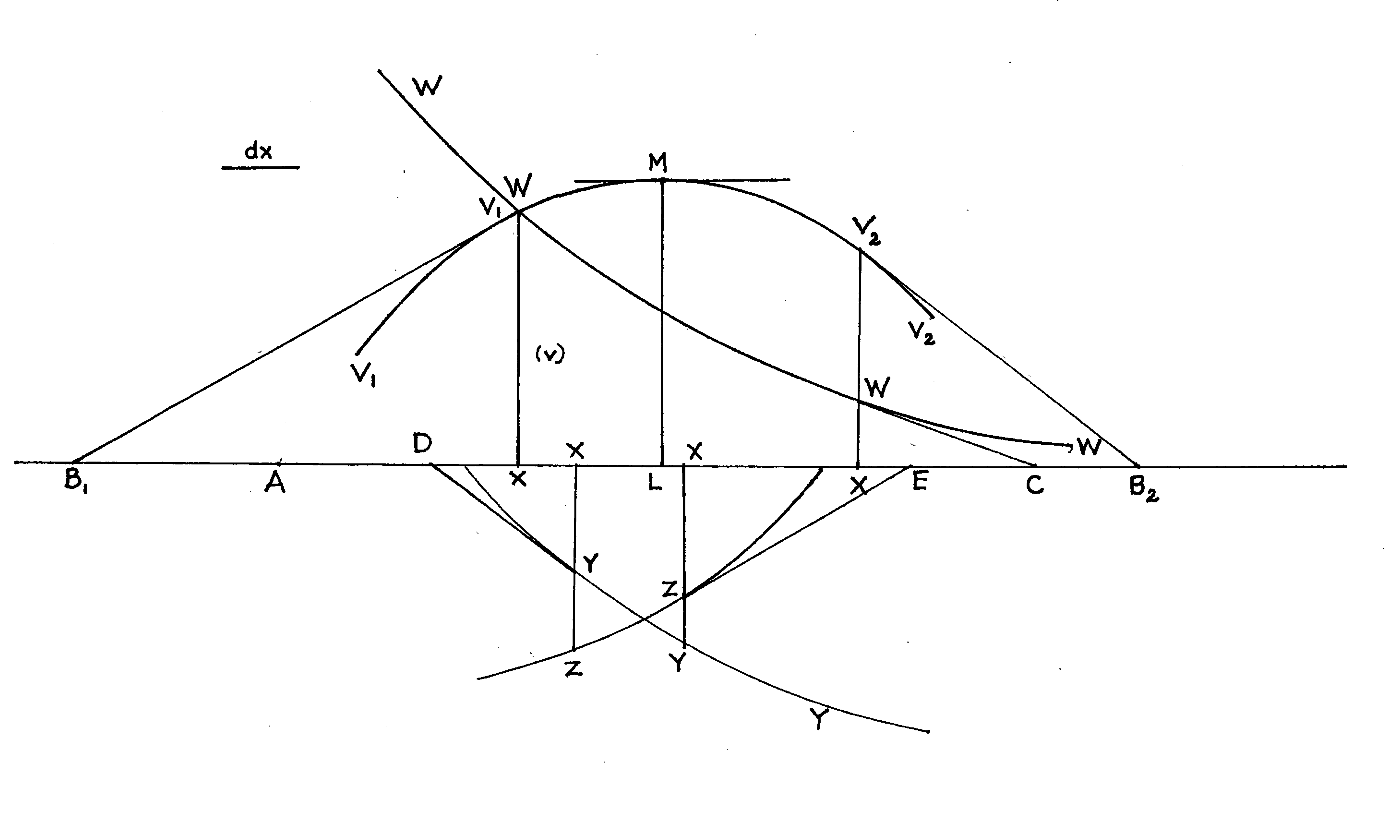
\includegraphics[scale=0.72]{fig/Figure2B} % This will put Figure 1 from "New Method" paper on the cover (in correct orientation).
    \end{figure}
    \vfill {\Large St.\ John's College, Annapolis\\[2ex]

      Fall Semester, 2022}
  \end{center}
\end{titlepage}

\tableofcontents



\section*{Selections from Aristotle's {\em Physics} to read with
  Galileo's {\em Two New Sciences}}%
%\addcontentsline{toc}{section}{\protect\numberline{1}{Selections from
\acl{Selections from Aristotle to read with Galileo} \pagestyle{plain}
\pagenumbering{arabic}

The following four passages on the infinite and continuity from
Aristotle's {\em Physics} may be useful in reading Galileo's {\em Two
  New Sciences}, pages~77--93.  The translations are by Joe Sachs
({\em Aristotle's Physics: A Guided Study}, 1995).

\begin{description}

\item[Book III, 206a7--b28] That, then, there is no actually infinite
  body, is clear from these things.  But that, if there is no infinite
  simply, many impossible things follow, is clear.  For there will be
  a beginning and an end of time, as well as magnitudes not divisible
  into magnitudes, and number will not be infinite.  But, whenever
  such a distinction has been made and neither way seems possible,
  there is a need for discrimination, and it is clear that in one way
  the infinite is, and in another way it is not.  Now being is said of
  what is potentially or of what is in complete activity, and there is
  an infinite by addition or by division.  And that there is no
  magnitude actually infinite has been said, but there is magnitude
  that is infinite by division; for it is not difficult to refute
  indivisible lines.  What is left, then, is that the infinite is as
  potentiality.  But it is necessary $|$\marginnote{206a20} not to
  take the being-potentially in the same way as if something were
  potentially a statue, since this will also \emph{be} a statue, and
  thus there would also be an infinite which would be at-work.  But
  since there are many ways of being, just as day is, or the athletic
  games which always come about one after the other, so also with the
  infinite. (For also with these things there is both
  being-potentially and being-at-work; for there are Olympic games
  both in the sense that the games are capable of happening and that
  they are happening.)  And this is evident in different ways in time,
  in human beings, and in the division of magnitudes. In general the
  infinite is in this way: it is in what is taken always one after the
  other, while what is taken is $|$\marginnote{206a30} always finite,
  but always another and another.  So being is meant in many ways, and
  the infinite must not be taken as a \emph{this,} such as a man or a
  house, but in the way that day or the games are meant, to which
  being belongs not as to a thing, but in a constant coming into being
  and passing away, finite, but always other and other.  But in
  magnitudes what is taken $|$\marginnote{206b1} remains, while with
  time and human beings it is always perishing in such a way as not to
  run out.

  But the infinite by addition is in some way the same as that by
  division, for the latter comes about in the finite by addition
  turned back the other way.  For where a division is seen to be to
  infinity, there is obviously an addition to what is cut off.  For if
  someone taking a marked-off part of a finite magnitude keeps taking
  from it in the same ratio (not including the piece of the whole
  magnitude already taken), the pieces will not exhaust the finite
  thing. $|$\marginnote{206b10} But if in the same way one increases
  the ratio so as always to include the same amount, they do exhaust
  it, through the whole finite thing's being used up by whatever part
  is marked off.  So it is in no other way, but in this way there is
  an infinite, in potentiality and by exhaustion (but it is also
  at-work, in the way we say day and the games to be).  And it
  \emph{is} thus in the way material is, potentially, and not on its
  own in the way the finite is.  And the infinite by addition is
  surely in potentiality in the same way, which we say is in a certain
  way the same as that by division.  For there will always be
  something outside to take, and it will not exceed
  $|${\reversemarginpar\marginnote{206b20}} every magnitude, just as
  in the division it does go beyond every marked-off piece and there
  will always be a smaller piece.

  Therefore to exceed everything by addition is not even possible
  potentially, unless there is accidentally an actual infinite, as the
  writers on nature say that which is outside the body of the cosmos,
  being of air or some other such thing, is infinite.  But if it is
  impossible for there to be an actually infinite sensible body in
  this way, it is clear that not even potentially could there be one
  by addition, other than in the way described, by a reversed
  division.

\item [Book III, 206b.33--207a.10] The infinite turns out to be the
  opposite of the way people speak of it.  For this is the infinite:
  not that outside of which there is nothing, but that outside of
  which there is always something.  Here is a sign: people speak of
  rings which do not have stone-settings as endless because there is
  always something beyond to take, speaking in accordance with a
  likeness though not strictly.  For it is necessary both that this
  condition be present and that at no time the same part be taken; but
  in the circle it does not happen that way, but only the succeeding
  part is always different.  Infinite, then, is that of which, to
  those taking it by quantities, there is always something beyond to
  take.  That of which nothing is outside is complete and whole; that
  is how we define the whole, as that of which nothing is absent, as a
  whole human being or box.

\item [Book V, 227a.10--17] That which, being next in series to
  something, is touching it, is next to it.  The continuous is that
  which is next to something, but I call them continuous only when the
  limits at which they are touching become one and the same, and, as
  the name [\foreignlanguage{greek}{suneq'hs}]
  implies, hold together
  [\foreignlanguage{greek}{sun'eqein}]. And this
  is not possible if the extremities are two.  And it is clear from
  this definition that the continuous is among those things out of
  which some one thing naturally comes into being as a result of their
  uniting.  And in whatever way the continuous becomes one, so too
  will the whole be one, such as by a bolt or glue or a mortise joint,
  or by growing into one another.

\item [Book VI, 232b.24--25] I call continuous that which is always
  divisible into divisible parts.

\end{description}



\section*{An Approach to the Arithmetic of Infinites: where we also show
   that a greatest number or an infinite number of all numbers is impossible
   or nothing; and show by examples that some things that are held to be
   axioms can be demonstrated}
\acl{Leibniz: An Approach to the Arithmetic of Infinites}

 
It has been established that the science of the least and the greatest, or of the
indivisible and the infinite, is among the greatest pieces of evidence which the human
mind uses in laying claim to its own incorporeality.  Who indeed, following his senses, could
persuade himself that there can be {\em given} no line so short that it does not contain both infinitely many points and also infinitely many lines (and
accordingly actually contains an infinite number of parts, all separated from each
other) having a finite ratio to the {\em given} line, if demonstrations did
not compel him?  And how truly wonderful it is to calculate the sum of
infinitely many decreasing quantities! or to prescribe limits to quantities
increasing or decreasing in a finite space! or to generate finite figures and
demonstrate their proportions by multiplying infinites by one another!\marginnote{Note 1, page~\pageref{caa1}}

Archimedes long ago used the arithmetic of infinites and the geometry of
indivisibles, as well as inscribed and circumscribed figures, in {\em The
Measurement of the Circle}, {\em On the Sphere and the Cylinder}, and {\em The
Quadrature of the Parabola}.  In our time, Cavalieri has revived the geometry
of indivisibles (while Galileo served as his midwife and gave his approval),
Wallis the arithmetic of infinites, and James Gregory inscribed and
circumscribed figures. And certainly, if a new light from indivisibles and
infinites does not shine on it and the art of analysis does not progress,
there is no hope of great progress in geometry.

The ancients have given us a rule for calculating a sum of fractions or ratios
decreasing indefinitely in a geometric progression. For if a quantity,
exhibited by the line $AB$ [see the diagram below], is
given, and this line is continually cut and recut so that the ratio of a
subsection, such as $AD$, to a section, such as $AC$, is as the ratio of the
section $AC$ to the whole, $AB$, or so that the ratios $\frac{AB}{AC} =
\frac{AC}{AD} = \frac{AD}{AE}$, etc., are equal; then, the ratio of $CB$ (the
remainder when the section $AC$ is taken away from the whole $AB$) to the
whole $AB$ will be the same as the ratio of the whole $AB$ to a whole composed
of the whole and in addition first the section, then the section of the
section, etc., all taken simultaneously; that is,
$$\frac{CB}{AB}= \frac{AB}{AB + AC + AD + AE + \mbox{etc.}}.$$

\begin{figure}
\begin{center}
\begin{picture}(250,95)
\thicklines

\put(0,10){A} \put(9,10){E} \put(27,10){D} \put(81,10){C} \put(243,10){B}

\put(0,20){ $\overbrace{
\begin{picture}(243,54)
\put(0,0){\line(1,0){243}} \put(243,0){\line(0,1){54}}
\end{picture}}^{1}$}

\put(249,45){1}

\put(0,20){ $\overbrace{
\begin{picture}(81,18)
\put(81,0){\line(0,1){18}}
\end{picture}}^{\frac{1}{3}}$}

\put(94,29){$\frac{1}{3}$}

\put(0,20){ $\overbrace{
\begin{picture}(27,6)
\put(27,0){\line(0,1){6}}
\end{picture}}^{\raisebox{-1pt}{\scalebox{.47}{{$\frac{1}{9}$}}}}$}
\thinlines \put(31,23){\line(3,1){10}} \put(42,26){$\frac{1}{9}$}

\thicklines \put(9,20){\line(0,1){2}} \put(0,22){\scalebox{.7}{etc.}}

\thinlines \put(9,22){\line(1,0){5}} \put(14,22){\line(1,-2){10}}
\put(24,1){\scalebox{.75}{$\frac{1}{27}$}}

\end{picture}
\end{center}
\end{figure}



I have seen a demonstration of this rule attempted by certain learned men, but
I have not seen an absolute demonstration; I not only demonstrate it from a universal principle\marginnote{Note 2, page~\pageref{caa2}} but
also draw from it
    an elegant consequence, namely: if we take continually decreasing
    fractions whose numerators are unity, but whose denominators are the terms
    in a certain geometric progression, then the sum of all the fractions of
    the given progression will be the first fraction of the preceding
    geometric progression, so that
\setlength{\jot}{2ex}
\begin{eqnarray*}
\frac{1}{2} + \frac{1}{4} + \frac{1}{8} \mbox{ etc.} & = & \frac{1}{1}\mbox{, and}\\
\frac{1}{3} + \frac{1}{9} + \frac{1}{27} \mbox{ etc.} & = & \frac{1}{2}\mbox{, and}\\
\frac{1}{4} + \frac{1}{16} + \frac{1}{64} \mbox{ etc.} &  = & \frac{1}{3},
\end{eqnarray*}
\setlength{\jot}{\oldjot}
 and so on.\marginnote{Note 3, page~\pageref{caa3}}

But this is not enough; let us go on to some things for which there are as yet
no rules.  I thought that I should write down for you, most distinguished
man,\footnote{Leibniz intended to send this manuscript to Jean Gallois, the editor of the \emph{Journal des S\c{c}avans}.} some ideas that came to my mind about
helping the arithmetic of infinites grow.

\label{beghar} When I once told the Illustrious Huygens that I had certain ways of summing a
few series that decreased indefinitely, and whose computation had not yet been
published, he proposed the following to me: he told me to look for the sum of
the fractions whose numerators are unity, but whose denominators are the
triangular numbers $0^1 1^2 3^3 6^4 10^5 15^6 21^7 28$ etc., namely, the numbers
whose differences are natural numbers.\marginnote{Note 4, page~\pageref{caa4}}  He said that once, when he was
thinking about calculations for dice and other games of chance, he needed this
sum and had found it, but it was not yet published.  I looked, and found that
the sum is binary, that is, $\frac{1}{1} + \frac{1}{3} + \frac{1}{6} +
\frac{1}{10} +\frac{1}{15} + \frac{1}{21} +\frac{1}{28} \mbox{ etc.} = 2.$
After I had shown this to Huygens, he admitted that it is true and also agrees
with his own calculation.

I, however, had found at the same time a universal method of summing series of
fractions or ratios not only of this progression of {\em triangulars}, where
the differences of terms are natural numbers, but also of {\em pyramidals},
where the differences of terms are triangular numbers, and of {\em
triangulo-triangulars}, where the differences are pyramidal, and of {\em
triangulo-pyramidals}, where the differences are triangulo-triangular, and of
{\em pyramido-pyramidals}, where the differences are triangulo-pyramidal, and
so on indefinitely.\marginnote{Note 5, page~\pageref{caa5}}  Examine Table\ 1.
\begin{table}
\begin{center}

\caption{}

\vspace{1ex}

\begin{tabular}{|rrrrrrrr|}\hline
\rule{0em}{8.25ex} {\rotatebox{90}{zero}} & & & & & & & \\ 0 &
{\rotatebox{90}{\makebox[0em][l]{units}}} & & & & & & \\ & 1 &
{\rotatebox{90}{\makebox[0em][l]{naturals}}} & & & & & \\ 0 & & 1 &
{\rotatebox{90}{\makebox[0em][l]{triangulars}}} & & & & \\ & 1 & & 1 &
{\rotatebox{90}{\makebox[0em][l]{pyramidals}}} & & & \\ 0 & & 2 & & 1 &
{\rotatebox{90}{\makebox[0em][l]{triangulo-triangulars}}} & & \\ & 1 & & 3 & &
1 & {\rotatebox{90}{\makebox[0em][l]{triangulo-pyramidals}}} & \\ 0 & & 3 & &
4 & & 1 & {\rotatebox{90}{\makebox[0em][l]{pyramido-pyramidals}}} \\ & 1 & & 6
& & 5 & & 1 \\ 0 & & 4 & &10 & & 6 & \\ & 1 & &10 & &15 & & 7 \\ 0 & & 5 & &20
& &21 & \\ & 1 & &15 & &35 & &28 \\ 0 & & 6 & &35 & &56 & \\ & 1 & &21 & &70 &
&84 \\ & & 7 & &56 & &126& \\ & & &28 & &126& &210\\ & & & &84 & &252& \\ & &
& & &210& &462\\ & & & & & &462& \\ & & & & & & &924\\ \hline
\end{tabular}
\end{center}
\end{table}

And these are the numbers whose series some call numerical orders, others
combinatoric orders, and others the numbers of a symmetric progression.
Pascal set forth their many uses in {\em The Arithmetic Triangle},
the treatise he wrote that is dedicated to them.\footnote{An excerpt of this treatise is translated into English by Anna Savitsky in D.\ E.\ Smith's {\em A Source Book in Mathematics}, 1929, pages 67--79.  The whole work, in Latin and French, is included Pascal's {\em Oeuvres}, Mesnard ed., vol.\ II, pp.\ 1166--1332, Descl\'ee de Brouwer, Paris, 1970.} I usually call them the
numbers of a {\em replicated arithmetic progression}; for any numbers whatever
(for example, binary or ternary numbers) can be substituted for the units,
while arbitrary numbers of an arithmetic progression beginning from its own
difference can be substituted for the natural numbers (for example, 2, 4, 6, 8
etc., for 1, 2, 3, 4, etc.), and the table will be proportionally the same;
indeed, if the generator is binary, we simply double all the terms, and if it
is ternary, we triple them, etc.  Moreover, we can make a universal rule for
the sums of fractions, whatever the generator may be, if only we understand
the numerator of the fractions to be the generator; for example, if the
generator is 2, we should substitute $\frac{2}{2} +\frac{2}{6} +\frac{2}{12}$
etc.\ for $\frac{1}{1} +\frac{1}{3} + \frac{1}{6}$ etc.  And after we divide
all the numbers in the former series by the generator, it is the same as the
latter.  

But as I was saying, there will be a rule for finding sums [see Table 2, below]: the sum of a series of fractions whose numerators are the generator, and whose
denominators are the terms of a certain replicated arithmetic progression, or,
what amounts to the same thing, the sum of ratios whose antecedents are unity,
and whose consequents are the terms of a certain replicated arithmetic
progression having unity as its generator---this sum, I say, is the fraction
or ratio whose numerator or antecedent is the exponent of the immediately
preceding series, that is, the penultimate series (taking the given
series as the ultimate series), but whose denominator or consequent is the
exponent of the series immediately preceding the preceding series, that is, of
the antepenultimate series.  By {\em exponent} I mean here the number of the
series or the ordinal number of its replication, namely, the number that
expresses the place of its replication in the series of replications.  Thus
the exponent in the first series, $\frac{1}{1}$, $\frac{1}{1}$, $\frac{1}{1}$,
etc., is 1, and the exponent in the second series, 1, 2, 3, 4, etc., is 2.
For while in the first series only the unit generator is repeated, in the
second the replications themselves or the repetitions are replicated, and in
the third, 1, 3, 6, 10, etc., the replications of the replications are
repeated; but if the generator is the unit, the number of a series or the
exponent of its degree coincides with the first number in it after the unit.
I call the number of the series its  {\em exponent} because I am following the example of the geometric
progression; in a geometric progression the exponent of the roots is 1, the exponent of the squares is 2,
the exponent of the cubes is 3, etc., just as in this case the exponent of the generators is 1, the exponent of
the naturals is 2, the exponent of the triangulars is 3, etc.

Therefore it follows that the sum of the series of triangular fractions
$$\frac{1}{1} + \frac{1}{3} + \frac{1}{6} + \frac{1}{10} +\frac{1}{15} +
\frac{1}{21} +\frac{1}{28} \mbox{ etc.}$$
 is $$=\frac{2}{1};$$ for the series
preceding the series 1, 3, 6 etc., namely 1, 2, 3 etc., has exponent 2, and
the series preceding {\em this} series, namely 1, 1, 1 etc., has exponent 1;
hence we get $\frac{2}{1}$ or 2.  And the sum of the series of pyramidal
fractions $$\frac{1}{1} + \frac{1}{4} + \frac{1}{10} + \frac{1}{20}
+\frac{1}{35} \mbox{ etc.}$$ is $$=\frac{3}{2},$$ or the ratio of the exponent of
the triangulars to the exponent of the naturals.

This is easier to see by looking at Table\ 2.\label{endhar}

\begin{table}
\begin{center}
\caption{Series of fractions of a replicated arithmetic progression}

\vspace{1ex}

\fbox{ \parbox{24.5em}{ $\begin{array}{cccccccccc}

\rule[-1.25ex]{0ex}{3.5ex} 0 & 1 & 2 & 3 & 4 & 5 & 6 & 7 & \mbox{etc.} &
\mbox{ exponents } \\ \hline

\rule[-2.75ex]{0ex}{6.5ex} \frac{0}{0} & \frac{1}{1} & \frac{1}{1} &
\frac{1}{1} & \frac{1}{1} & \frac{1}{1} & \frac{1}{1} & \frac{1}{1} & & \\

\rule[-2.75ex]{0ex}{5.5ex} \frac{0}{0} & \frac{1}{1} & \frac{1}{2} &
\frac{1}{3} & \frac{1}{4} & \frac{1}{5} & \frac{1}{6} & \frac{1}{7} & & \\

\rule[-2.75ex]{0ex}{5.5ex} \frac{0}{0} & \frac{1}{1} & \frac{1}{3} &
\frac{1}{6} & \frac{1}{10} & \frac{1}{15} & \frac{1}{21} & \frac{1}{28} & & \\

\rule[-2.75ex]{0ex}{5.5ex} \frac{0}{0} & \frac{1}{1} & \frac{1}{4} &
\frac{1}{10} & \frac{1}{20} & \frac{1}{35} & \frac{1}{56} & \frac{1}{84} & &
\\

\rule[-2.75ex]{0ex}{5.5ex} \frac{0}{0} & \frac{1}{1} & \frac{1}{5} &
\frac{1}{15} & \frac{1}{35} & \frac{1}{70} & \frac{1}{126} & \frac{1}{210} & &
\\

\rule[-2.75ex]{0ex}{5.5ex} \frac{0}{0} & \frac{1}{1} & \frac{1}{6} &
\frac{1}{21} & \frac{1}{56} & \frac{1}{126} & \frac{1}{252} & \frac{1}{462} &
& \\

\rule[-2.25ex]{0ex}{5.0ex} \frac{0}{0} & \frac{1}{1} & \frac{1}{7} &
\frac{1}{28} & \frac{1}{84} & \frac{1}{210} & \frac{1}{462} & \frac{1}{924} &
& \\ \hline

\rule[-1.75ex]{0ex}{5.0ex} \frac{0}{0} & \frac{0}{0} & \frac{1}{0} &
\frac{2}{1} & \frac{3}{2} & \frac{4}{3} & \frac{5}{4} & \frac{6}{5} &
\mbox{etc.} & \mbox{ sums } \\

\end{array}$}
\hspace{-5.5em} \raisebox{1ex}{\parbox{5.5em}{ \rotatebox{90}{\parbox{15em}
{\begin{center} Series of fractions of a replicated arithmetic progression
with unit generator
\end{center}
}}}}}
\end{center}
\end{table}

But since such a method of finding and demonstrating is quite lengthy and
requires many lemmas, I will wait until I have more time to put it in order
before I publish it, along with many other things of the same
kind.\marginnote{Note 6, page~\pageref{caa6}}


Yet I cannot pass up here a chance I have to make a certain point about the
nature of the {\em infinite number of all numbers}.  Galileo\footnote{In the {\em Two New Sciences}, First Day, on page 83 in Volume VIII of Galileo's {\em Opere}, edited by A.\ Favaro; on Page 45 in Stillman Drake's translation, Toronto, 1989.} compares it to the {\em unit}, and he reasoned as follows:
every number indefinitely has its own square, its own cube, etc; for if it is
multiplied by itself, its square, cube, etc.\ is produced; therefore there are
as many cubes and as many squares as there are roots or simple numbers, which
is impossible; for there are always many other non-squares placed between the
square numbers, and still more non-cubes between the cubes.  What then?  Do
the attributes ``equal'' and ``greater'' or ``less'' have no place in the
infinite?  He also suggests that, if any number is infinite, the unit is; for
it has that property that the infinite number of all numbers needs to have:
that there are as many roots in it as squares and cubes; for the square and
cube etc.\ of the unit is the unit.  I, however, conclude that if there is any
such infinite number, it is zero or nothing, or, what amounts to the same
thing, that such a number is nothing or = 0.

Such an infinite number has not only the property that Galileo observed in it
---that there are as many powers of every kind in it as there are roots---but also the property that there are in it as many numbers taken simply, that
is, both evens and odds together, as there are even numbers. For the even
numbers are the doubles of the numbers taken simply, yet there are as many
simple numbers as there are doubles of them.  In the same way we conclude that
there are not only as many numbers taken simply as there are even numbers
(binaries), but also as many as there are ternaries (triples of numbers taken
simply), and as there are quaternaries, etc., and triangulars, pyramidals,
etc. In the same way we prove that there are as many numbers taken simply as
there are numbers of any given progression, arithmetic, geometric, or mixed,
or of any replicated progression going on indefinitely; although it is more
than manifest that between the binaries or evens there are other, odd,
numbers, and that there are still more non-ternary numbers between the
ternaries.  Therefore, since in such an infinite number there are as many even
numbers as there are odd and even numbers together, that is, as many as there
are numbers taken simply, it follows that in such an infinite number the axiom
that the whole is greater than the part fails (just as Gregory of St.\ Vincent
contends that it fails for the angle of contact\footnote{Gregory apparently argued that the angle formed by a diameter of a circle and a tangent at its endpoint is not greater than the curvilineal angle formed by the same diameter and the circumference.  In the diagram to Euclid's {\em Elements}, Proposition III 16, Gregory would say that the whole right angle $BAE$ is not greater than its part, the curvilineal angle $BAHC$.}).  But it is impossible for
this axiom to fail, or, what amounts to the same thing, such an axiom never
fails, that is, it fails for {\em nothing}.  Therefore such an infinite number
is impossible---not one, not whole, but nothing.  Therefore such an infinite
number = 0.  And in 0 or zero we certainly find not only the property noticed
by Galileo in the unit, but also all the rest; for the square and cube of 0 is
0, and the double and triple of 0 is 0, and 0 + 0 is = 0, the whole to the
part.  And, so as not to seem to digress too far from the matter at hand, I
confirm this by gathering into a sum a series that progresses indefinitely;
for when we sum the fractions of a geometric progression it is certain that
the sum of any series is the first fraction of the preceding series, and
$\frac{1}{3} + \frac{1}{9} +\frac{1}{27} \mbox{ etc.} = \frac{1}{2}$, and
likewise $\frac{1}{2} + \frac{1}{4} +\frac{1}{8} \mbox{ etc.} = 1$, and
therefore $\frac{1}{1} + \frac{1}{1} +\frac{1}{1} \mbox{ etc.} = 0$.  Now $1 +
1 + 1$ etc.\ constitutes the infinite number of all numbers.  The same thing
happens in the above table of the fractions of a replicated arithmetic
progression, where it is clear that $\frac{1}{1} + \frac{1}{2} +\frac{1}{3}
\mbox{ etc.} = \frac{1}{0}$ and $\frac{1}{1} + \frac{1}{1} +\frac{1}{1} \mbox{
etc.} = \frac{0}{0} = 0$.

The same topic should remind us that, if we are going to be rigorous, if
philosophy is to be perfected, we should accept no proposition unless it
either agrees with an immediate sense-observation or is demonstrated from
clear and distinct imagination, that is, from an {\em idea}, or from a
definition (which is what idea signifies).  Obviously the definitions
themselves need not be demonstrated, since, as the restorer of philosophy
Galileo has emphasized so many times in his writings, they are arbitrary, and
cannot be charged with falsity, but only with unsuitability and obscurity.

Since such a proposition---that the whole is greater than the part---has
been doubted by the greatest geometers, including Galileo and Gregory of
St.\ Vincent, shall we continue to proclaim that there are other propositions
that are known through themselves?

Galileo certainly believed that an infinite number is something or one whole,
for he compares it to a unit; but nevertheless he denies that being greater
and being less have any place in it; for he denies that there are more numbers
taken simply, that is, squares and the non-squares, than there are square
numbers, or that the whole is greater than the part.

Hobbes erred in concluding that the truth of all propositions comes from human
decision.\footnote{Hobbes concludes something like this in {\em On Body} (the first part of his {\em Elements of Philosophy}), Chapter 3, Paragraph 8. } For, first of all, we should leave out those propositions which are
established by sense-perception, such as the proposition that I am {\em
sensed} by myself as sensing; but we should also leave out those propositions
that we demonstrate by applying definitions to what we know---for example,
when we demonstrate from the preceding proposition that I {\em sense} or
think, and likewise that I {\em am}.  For it is certain by sense-perception
that I am sensed by myself as sensing, and therefore that {\em I, as sensing}
am sensed immediately (without any medium); for between myself and me, in the
mind, there is no medium.  Whatever is immediately sensed is immediately
sensible.  Whatever is immediately sensible is sensible without error (for all
error is from a medium of sensation---I am supposing this as something that
is to be demonstrated elsewhere).  Whatever is sensible without error, is;
hence it follows that {\em I am sensing}, that is, that the proposition, ``I
am {\em sensing},'' is true.  Consequently I reflect: ``{\em I am sensing}.''
We should also leave out identical propositions or the affirmation of the same
thing about the same thing with the same words. But when we say the same thing
about the same thing with equivalent words---for example, when we say the
definition of something, or when we take different definitions of the same
thing and apply them to each other in turn, or when we take a part of one
definition of something and apply it to that thing or to some other definition
of it---it is manifest that the truth of our proposition is by human
decision; for definition is by human decision.  And all axioms that do not
depend on sense-perception---indeed all theorems in the sciences that are
independent of sense perception and experience---are propositions of this
sort, as Aristotle also noticed, who set down {\em definition} as the unique
principle of demonstration.\footnote{See {\em Posterior Analytics} II 3, 90b25.}  And in fact all the axioms that Euclid puts at
the beginning of his elements are demonstrable from definitions.  ``Then,''
you will say, ``what are we learning when we investigate the theorems of such
sciences?''  Nothing, I would say, except how to think more quickly and
distinctly for practical purposes, or how to use certain fitting symbols to
order thoughts we have had and ideas we have received through our
senses. (These symbols may be either names or characters.) Consider, for
example, numbers; who does not see that we learn nothing new in all of
arithmetic except the names of numerals and their various recursions, which
become harmonic if they are inverted; from here we draw out equations as
theorems and it then becomes very clear how useful characters are, when by
using the symbols we have made we can notice much that we would not otherwise
have seen---for example, when we easily calculate the sum of an entire
progression.  And this is most apparent in algebra, where no one does not see
that we do everything by means of symbols variously transposed, and reap a
prodigious harvest, not because we learn new things, but because things are
shown naked to the mind.  In the same way, if we were to have a philosophical
language or at least a philosophical writing, which I spoke about in the {\em
Combinatoric Art},\footnote{A work Leibniz published in 1666.  It is reprinted in Volume 1 of Series VI the Berlin Academy edition of Leibniz's collected works.  The relevant passage is in sections 89 and 90. } and which would use the
elements of thinking instead of an alphabet, we could write things down by
means of their definitions.  And just as in algebra there are equations
everywhere, here there would be theorems everywhere, and we could propose and
solve infinitely many problems and demonstrate theorems with no trouble, and
it would be impossible for anyone who does not understand things to use this
writing, and everyone would be able to reason without error, as in arithmetic.
And algebra, both numerical and specious, is only a part or an example of this
universal writing or philosophic characterism; I wonder why this has not been
sufficiently noticed by the greatest men.  I, however, am preparing an example
in morality or justice, in order that it may appear---


Since I have ascertained that every whole is greater than its part, I boldly
conclude that such an infinite number or greatest number or sum of all
possible units, which you may also call most infinite or the number of all
numbers, is 0 or nothing.  And we can give a new demonstration, for instance
by using the fact that a greatest number is the sum of all units or the number
of all numbers.  And the sum of all numbers is necessarily greater than the
number of numbers (as $1+2+3$ etc.\ is greater than $1+1+1$ etc.).  Therefore,
the greatest number is not the greatest number, that is, the greatest number
is 0, although I would not therefore straightaway deny that there are
infinitely many parts in the continuum or that there is an infinite magnitude
in time or space.

Hence it appears that such propositions as: that things equal to the same
thing are also equal to each other; that equals added to or taken away from
equals make equals; that the whole is greater than the part; that
equimultiples are as simples; that if proportionals are added or taken away
from proportionals, proportionals are produced, etc.\---since these all can
be doubted, they must be demonstrated, and accordingly, if they are true, they
are demonstrable (from terms or definitions, of course).  And the scholastics
wished that first truths might become known through inspection of terms, that
is that they might be easy to demonstrate and almost definitions; on the other
hand there are those who think that these first truths are known through
themselves, by means of I know not what natural light.  For it is well known
that some things are placed by some men among the things known through
themselves, while the same things are rejected and distinguished from them by
others, and that men have no criterion to decide what is known through itself,
except perhaps common opinion, which, besides being exposed to doubt, would
set down probable things as the foundations of demonstrations, which is to
give way to the Pyrrhonists.

``But indeed,'' someone will say, ``if all axioms are demonstrable from
definitions of names, all truths will depend on human decision, since the
definitions of names are arbitrary; but this opinion in Hobbes is condemned by
the learned.''  I reply that propositions depend on definitions to the extent
that they are expressed by words and other symbols, but asymbolic thoughts,
that is, the connexions of the ideas themselves, are either from sense
perception or from distinct imagination.  (We have a distinct imagination when
we distinguish a subject matter into parts by examining it and considering it
through its circumstances, as long as nothing new happens that is relevant to
the matter at hand.)  Hence the theorems change as relations change, just as
the same city changes its shape depending on which side we see it from.  It
therefore seems to me that one must distinguish between propositions; for the
truth of some, such as those that are based on experiments and observations of
nature, depends upon sense-perception, while the truth of others, such as the
theorems of arithmetic and geometry, depends upon a clear and distinct
imagination or ideas or, if you prefer, definitions (for definition is nothing
other than the signification of ``idea'').  Therefore signs and symbols,
whether they are words or characters, are arbitrary, but all nations have the
same ideas.  Yet in reasoning about very complex things we are accustomed to
use symbols, without considering the ideas themselves.  These {\em thoughts}
are {\em blind}, since in them we are content with an analogy with small and
simple thoughts distinctly comprehended.  For example, when we say
``100,000,'' no one forms all its units in his mind; for he knows that by
doing this he can leave them behind the symbols.  And the art of devising
symbols consists in this: that they be briefer than the ideas themselves and
yet free from confusion and suited to revealing (to the extent that this is
possible) proportions of every kind in those very ideas no less easily than if
they had been resolved into ultimate elements or had been clearly and
distinctly understood.  And the decimal progression does this quite well for
numbers; for without a progression like this it would have been too tedious
for mortals to count up huge numbers.  Algebra does the same thing for
geometry, so that even when we assume impossibilities, such as dimensions
beyond the third and surd\footnote{Surd numbers are irrational numbers, that is, numbers that are not equal to fractions where both the numerator and denominator are whole numbers.  $\sqrt{2}$ is an example of a surd number.  The Latin word ``surdus," which Leibniz uses here, literally means mute.} numbers and numbers less than nothing, it
nevertheless succeeds.

Therefore, since when we have found suitable symbols they support our mind
like spiritual machines, but those symbols we have now, except in the pure
mathematical sciences (although even there I could wish for more), are neither
simple, nor complete, nor ordered, it appears that no one would be more
deserving in the whole realm of human reasoning than someone who could devise
either a philosophical language or at least a writing to serve for rigorous
investigations.  I stated this six years ago in the {\em Dissertation on the
Combinatoric Art}, which, although it is a childish work written in an
academic manner, I will nevertheless not entirely scorn now.  There I pointed
out that all propositions of the pure sciences, that is, those independent of
sense-perception (although we can also, as it were, examine and confirm their
truth by sense-perception), which include also the sciences of action in
general, of reasoning, of motion, of utility, and of justice, do nothing but
pronounce either a definition or a part of a definition (or a definition of a
part or a part of a part, wholly or in part) about something that is defined
or about some other definition of the same thing. And I pointed out that the
same idea can be expressed by various definitions and this gives birth to a
fertile art for constructing theorems.  I remember Pascal saying the same
thing somewhere or another,\footnote{In the {\em Trait\'{e} des Ordres Num\'{e}riques} ({\em Treatise on Numerical Orders}), {\em Oeuvres}, Mesnard edition, volume II, page 1329.}  where he recommends that we give varied
enunciations of the same theorems and says that the whole study of geometers
should consist in this; for thus, he says, we open a way to new and untouched
things.  Cujas, in his Paratitla, also observed that we can usefully propose
many definitions of the same name; indeed, definitions in that universal
characteristic\marginnote{Note 7, page~\pageref{caa7}} are the same as equations in algebra.

But let us show, by the deed itself, rather than by words, the demonstrability
of the axioms we set out as examples.
\begin{description}
\item[First:] {\em that things equal to the same third thing are equal to each
other}.  We immediately understand this axiom from the definition of equality.
For let $a=b$ and $b=c$; I say $a=c$.  For things are {\em equal} which have
the same quantity or which can be substituted for each other while preserving
the quantity; therefore let us substitute either $c$ in place of $b$ in the
equation $a=b$ or $a$ in place of $b$ in the equation $b=c$, and either way we
will have $a=c$.  \textsc{q.e.d.}
\item[Second:] {\em that equals added to or subtracted from equals make
equals.}  $a=b$ and $c=d$. I say that $a+c= b+d$.  For $a+c = b+c$ (because
$a=b$) and $b+c = b+d$ (because $c=d$). Therefore $a+c = b+d$.
\item[Third:] {\em that the whole is greater than the part.}  For if (def. 1)
the parts are $a$, $b$, the whole (def. 2) will be $a+b$.
\begin{center}
\fbox{
\begin{picture}(130,54)

\thicklines \put(37,43){a} \put(90,43){b} \put(15,33){\line(1,0){50}}
\put(70,33){\line(1,0){5}} \put(80,33){\line(1,0){5}}
\put(90,33){\line(1,0){5}} \put(100,33){\line(1,0){5}}
\put(110,33){\line(1,0){5}} \put(15,18){\line(1,0){100}} \put(63,8){c}

\end{picture}}
\end{center}
Again, if $a$ is less (def. 3), then $c=a+b$ will be {\em greater} (def. 4).\marginnote{Note 8, page~\pageref{caa8}}
If we put the definitions together the demonstration will complete: the
{\em whole} $= a + b$ (def. 2), $a + b = c$ (def. 4), $c =$ greater (def. 4),
the part $= a$ (def. 1), and $a = $ less (def. 3).

\item[Fourth:] {\em that equimultiples are as simples}; e.g., as three are to
four, so are twice three to twice four.

$\frac{ca}{cb} =\frac{a}{b}$. For $\frac{ca}{cb} = \frac{c}{c} \cap
\frac{a}{b}$.  Now $\frac{c}{c} = 1$ and $1 = \frac{1}{1}$, and therefore
$$\frac{ca}{cb} = \frac{1}{1} \cap \frac{a}{b} = \frac{1a}{1b} =
\frac{a}{b}.$$

So that there cannot be any doubt left, I prove that $\frac{ca}{cb} =
 \frac{c}{c} \cap \frac{a}{b}$ as follows:
$$\frac{c}{c} \cap \frac{a}{b} = \frac{c \cap \frac{a}{b}}{c} =
\frac{\frac{ca}{b}}{c} = \frac{ca}{cb}.$$ Here $\cap$ is the multiplication
sign.

\item[Fifth:] {\em that if proportionals are added or taken away from
proportionals, proportionals are produced.}  For example, since 4 is to 8 as 3
is to 6, so 4+3, or 7, will have the same ratio to to 8+6, or 14; that is, if
$\frac{a}{b} = \frac{c}{d}$, then they both $= \frac{a+c}{b+d}$.  But first of
all let me demonstrate this {\em lemma}: $bc = ad$; for because $\frac{a}{b} =
\frac{c}{d}$, by multiplying each side by $d$, $\frac{ad}{b}$ will be
$=\frac{c}{1}$, and therefore by multiplying each side by $b$, we will have
$ad = bc$.  Now, continuing, if
$$\frac{a+c}{b+d} \times \frac{a}{b} =1,$$ then will\marginnote{Note 9, page~\pageref{caa9}}
$$\frac{a+c}{b+d} = \frac{a}{b}.$$ That the latter equation follows from the
former is obvious; for
$$\frac{a+c}{b+d} \times \frac{a}{b} = \frac{a+c}{b+d} \cup \frac{a}{b} =
\frac{a+c \cup \frac{a}{b}}{b+d}$$
$$=\frac{a +c \cup a \cup \frac{1}{b}}{b + d} = \frac{a+ c \cap b \cup
\frac{b}{b}}{b + d \cap a} = \frac{a + c \cap b \cup 1}{b + d \cap a}$$
$$= \frac{a + c \cap b}{b + d \cap a} = \frac{a + c}{b +d} \times
\frac{a}{b}.$$

I prove the former equation as follows:
$$\frac{a + c}{b + d} \times \frac{a}{b} = \frac{ba + bc}{ab + ad},$$ and
because, by the preceding lemma, $bc = ad$, it follows that
$$\frac{ba + bc}{ab + ad} = \frac{ba + bc}{ab + bc} = 1.$$

From this last example we see that this proposition, which we made our fifth
axiom, is no easier to demonstrate than some others that are counted as
theorems. For example, it is a theorem that {\em if two ratios are equal,
their inverses are also equal.}  We easily demonstrate this as follows:
$\frac{a}{b} = \frac{c}{d}$, I say $\frac{b}{a} = \frac{d}{c}$.  For if
$\frac{b}{a} \times \frac{d}{c} = 1$, then will $\frac{b}{a} = \frac{d}{c}$.
I prove the former equation as follows: $\frac{b}{a} \times \frac{d}{c} =
\frac{bc}{da} = \frac{bc}{bc} = 1$; for by the stated lemma $da = bc$.

\end{description}

These examples should be enough to support our observation---an observation
that, although it is scarcely believed, is nonetheless necessary to establish
the rigor of the sciences against the Pyrrhonists.

\newpage

\section*{Notes on Leibniz's ``An Approach to the Arithmetic of Infinites''}
\acl{Notes on Leibniz's ``An Approach to the Arithmetic\\ of Infinites''}

Leibniz wrote this paper for the {\em Journal des S\c{c}avans} (Journal of the Learned) in late 1672.   The paper is written in Latin, and we have translated it from a text published in 1976 in an edition of Leibniz's collected works put out by the Berlin Academy of Sciences, the  {\em S\"{a}mtliche Schriften und Briefe} (Collected Writings and Letters), in Series~III, Volume~1, on pages 1--20. 

\subsection*{Note 1}
\label{caa1}

In a short text titled ``On the Use and Necessity of Demonstrations of the Immortality of the Soul," Leibniz says more about how the incorporeality of the soul is connected to the science of the indivisible and the infinite:
\begin{quote}
But I shall say nothing about Mind except what can be both clearly perceived and distinctly demonstrated.  What I shall say about Mind will be no more difficult than what geometers say about a point and angles.  Indeed, the theory of points and angles, of the instant, of endeavor (by {\em endeavor} I mean a last or least motion, that is, a motion which happens in an instant, within a point), will be for me the key to explaining the nature of thought.  For I shall demonstrate that Mind exists in a point, that thought is endeavor or least motion, and that a body may have many endeavors at one time, although it has only one motion.  Whence it will follow that a mind may no more be destroyed than a point.  For a point is indivisible, and therefore cannot be destroyed.  Therefore though a body may be burned up and scattered to all the corners of the earth, the Mind will remain safe and untouched in its point.  For who will burn up a point?\footnote{See Series II, volume 1, page 113, of the Berlin Academy's edition of Leibniz's collected works. This text was written in 1671.} 
\end{quote}


In this first paragraph of ``An Approach to the Arithmetic of Infinites," Leibniz briefly alludes to four examples.  It is not necessary to understand these examples to go on, but it may be helpful to say a few words about them here.
\begin{enumerate}
\itemsep0em
\item Any line can be cut into infinitely many separate lines.
\item We can ``calculate the sum of infinitely many decreasing quantities."  Leibniz will give a few examples of this later in the paper.
\item We can ``prescribe limits to quantities increasing or decreasing in a finite space."  Here Leibniz may be thinking of constructions like those in Proposition 2 of Book XII of Euclid's {\em Elements}.  There Euclid shows how to construct an infinite series of polygons inscribed in a circle, such that each polygon contains the the previous polygon in the series.  These inscribed polygons are ``quantities increasing \ldots in a finite space," and the limit which is prescribed for them is the circle.  Similarly, Euclid shows in the same proposition how to construct an infinite series of polygons circumscribed around a circle, such that each polygon is contained by the previous polygon in the series.  These circumscribed polygons are ``quantities decreasing in a finite space," and the limit which is prescribed for them is again the circle.
\item We can``generate finite figures and
demonstrate their proportions by multiplying infinites by one another."   Infinites may be used to find proportions between curvilinear figures.   Here is an argument using infinity to find the area of circle:\footnote{This passage is from the the Santa Fe Junior Mathematics Manual (2007 edition, page~12).  It appears to be quoted from {\em The Mathematical Experience}, by Philip J. Davis and Reuben Hersh (on pages 262 and 263 of the 1995 study edition, published by Birk\"{a}user). Davis and Hersh attribute the quote to Nicholas of Cusa, but do not give a reference.}
\begin{quote}
We wish to find the relation between the area of a circle and its circumference. For
simplicity we suppose that the radius of the circle is 1. Now, the circle can be thought of
as  composed of infinitely many straight-line segments, all equal to each other
and infinitely short. The circle is then the sum of infinitesimal triangles, all of which
have altitude 1. For a triangle the area is half the base times the altitude. Therefore the
sum of the areas of the triangles is half the sum of the bases. But the sum of the areas of
the triangles is the area of the circle, and the sum of the bases of the triangles is its
circumference. Therefore the area  of the circle of radius 1 is equal to one half its
circumference.
\end{quote}
In taking a circle to be a sum of infinitely many infinitely small triangles, we may be said to generate it by multiplying an infinite (one triangle, which is infinitely small) by another infinite (the number of these triangles).
\end{enumerate}

\subsection*{Note 2}
\label{caa2}

Leibniz does not give a demonstration of this rule in this paper, but here is a roughly Euclidean demonstration.
We first note that
$$CB + DC + ED + \mbox{ etc.} = AB.$$

Next, according to Proposition 19 in Book V of Euclid's {\em Elements}, because 
$$AB\!:\!AC :: AC\!:\!AD,$$
it follows that 
$$(AB-AC)\!:\!(AC-AD) :: AB\!:\!AC\mbox{, that is, } CB\!:\!DC :: AB\!:\!AC.$$
Alternating (Euclid, V 16), we get
$$CB\!:\!AB :: DC\!:\!AC.$$
Similar arguments show that 
$$ DC\!:\!AC :: ED\!:\!AD.$$  We could go on indefinitely in the same way, getting an infinite series of proportions:
$$CB\!:\!AB :: DC\!:\!AC :: ED\!:\!AD \ldots$$


Now according to Euclid V 12, ``if any number of magnitudes be proportional, as one of the antecedents is to one of the consequents, so will all the antecedents be to all the consequents."  If we suppose Euclid's proposition is true not only for any {\em finite} number of magnitudes, but also for an {\em infinite} number of magnitudes, then as one of the antecedents ($CB$) is to one of the consequents ($AB$), so will all of the antecedents ($CB + DC + ED +$ etc.) be to all of the consequents ($AB + AC + AD + AE +$ etc.).  Expressing this proportion in a equation, we get:
$$\frac{CB}{AB} = \frac{CB + DC + ED + \mbox{ etc.}}{AB + AC + AD + \mbox{ etc.} } = \frac{AB}{AB + AC + AD + \mbox{ etc.}}$$
This is Leibniz's equation.

\begin{figure}
\begin{center}
\begin{picture}(250,95)
\thicklines

\put(0,10){A} \put(9,10){E} \put(27,10){D} \put(81,10){C} \put(243,10){B}

\put(0,20){ $\overbrace{
\begin{picture}(243,54)
\put(0,0){\line(1,0){243}} \put(243,0){\line(0,1){54}}
\end{picture}}^{1}$}

\put(249,45){1}

\put(0,20){ $\overbrace{
\begin{picture}(81,18)
\put(81,0){\line(0,1){18}}
\end{picture}}^{\frac{1}{3}}$}

\put(94,29){$\frac{1}{3}$}

\put(0,20){ $\overbrace{
\begin{picture}(27,6)
\put(27,0){\line(0,1){6}}
\end{picture}}^{\raisebox{-1pt}{\scalebox{.47}{{$\frac{1}{9}$}}}}$}
\thinlines \put(31,23){\line(3,1){10}} \put(42,26){$\frac{1}{9}$}

\thicklines \put(9,20){\line(0,1){2}} \put(0,22){\scalebox{.7}{etc.}}

\thinlines \put(9,22){\line(1,0){5}} \put(14,22){\line(1,-2){10}}
\put(24,1){\scalebox{.75}{$\frac{1}{27}$}}

\end{picture}
\end{center}
\end{figure}

\subsection*{Note 3}
\label{caa3}

We can obtain these sums by substituting in numerical values for the lines $AB$, $AC$, $AD$, etc.  To get the first sum, let $AB = 1$ and $AC = \frac{1}{2}$.  Then $AD$ is likewise half of $AC$  (because
$AD\!:\!AC :: AC\!:\!AB$), and $AE$ is half of $AD$, and so on; therefore
 $$AD = \frac{1}{4} \mbox{, } AE = \frac{1}{8} \mbox{, etc.}$$ 
   Then $CB = AB - AC = 1- \frac{1}{2} = \frac{1}{2}.$  We substitute all these values into Leibniz's equation,
   $$\frac{CB}{AB}= \frac{AB}{AB + AC + AD + AE + \mbox{etc.}},$$
   to get
$$\frac{\frac{1}{2}}{1} = \frac{1}{1 + \frac{1}{2} + \frac{1}{4} + \frac{1}{8} + \mbox{ etc.}}$$
Inverting both sides, we get
$$ \frac{2}{1} = 1 + \frac{1}{2} + \frac{1}{4} + \frac{1}{8} + \mbox{ etc.}$$
Dividing both sides by 2, we get
$$\frac{1}{1} = \frac{1}{2} + \frac{1}{4} + \frac{1}{8} + \frac{1}{16} \mbox{ etc.,}$$
which is Leibniz's first sum.  To get the second and third sums, we proceed in the same way, but set $AC= \frac{1}{3}$ and $AC = \frac{1}{4}$, respectively.

\subsubsection*{Problem 1}\label{geosum}

Show that if $AB =1$ and $AC = x$, then 
$$\frac{1}{1-x} = 1 + x + x^2 + x^3 + \mbox{ etc.}$$

\subsection*{Note~4}
\label{caa4}

Leibniz's notation here may be confusing.  The triangular numbers are simply the numbers 0, 1, 3, 6, 10, 15, 21, 28, etc.  The numbers 1, 2, 3, 4, 5, 6, and 7, written between and above the triangular numbers, are the differences of the pairs of consecutive triangular numbers: the difference of 0 and 1 is 1, the difference of 1 and 3 is 2, the difference of 3 and 6 is 3, etc.

Triangular numbers may also be defined as numbers whose units may be evenly arranged into equilateral triangles.  This is the way Nicomachus defines them, in Book II, Chapter 8 of his {\em Introduction to Arithmetic}. 

\begin{table}
\begin{center}

\caption{}

\vspace{1ex}

\begin{tabular}{|rrrrrrrr|}\hline
\rule{0em}{8.25ex} {\rotatebox{90}{zero}} & & & & & & & \\ 0 &
{\rotatebox{90}{\makebox[0em][l]{units}}} & & & & & & \\ & 1 &
{\rotatebox{90}{\makebox[0em][l]{naturals}}} & & & & & \\ 0 & & 1 &
{\rotatebox{90}{\makebox[0em][l]{triangulars}}} & & & & \\ & 1 & & 1 &
{\rotatebox{90}{\makebox[0em][l]{pyramidals}}} & & & \\ 0 & & 2 & & 1 &
{\rotatebox{90}{\makebox[0em][l]{triangulo-triangulars}}} & & \\ & 1 & & 3 & &
1 & {\rotatebox{90}{\makebox[0em][l]{triangulo-pyramidals}}} & \\ 0 & & 3 & &
4 & & 1 & {\rotatebox{90}{\makebox[0em][l]{pyramido-pyramidals}}} \\ & 1 & & 6
& & 5 & & 1 \\ 0 & & 4 & &10 & & 6 & \\ & 1 & &10 & &15 & & 7 \\ 0 & & 5 & &20
& &21 & \\ & 1 & &15 & &35 & &28 \\ 0 & & 6 & &35 & &56 & \\ & 1 & &21 & &70 &
&84 \\ & & 7 & &56 & &126& \\ & & &28 & &126& &210\\ & & & &84 & &252& \\ & &
& & &210& &462\\ & & & & & &462& \\ & & & & & & &924\\ \hline
\end{tabular}
\end{center}
\end{table}


\subsection*{Note 5}
\label{caa5}

Each number in this table is equal to the difference of the two nearest numbers to its right.  For example, the triangular number 6 is equal to the difference of the pyramidal numbers 10 and 4, the triangulo-pyramidal 252 is equal to the difference of the pyramido-pyramidals 462 and 210, etc.  Or, what amounts to the same thing, each number is the sum of the number above it and the number above it and to its left: $10= 6+4$, $462 = 252 + 210$, etc. This gives an easy way to generate all the entries in the table by adding.  For example, to fill in one more row in the table, we note that the next natural number after 7 is 8, and therefore the next triangular number after 28 must be $28+8 = 36$, the next pyramidal number after 84 must be $84 + 36 = 120$, the next triangulo-triangular number after 210  must be $210 + 120 = 330$, etc.  We could go on indefinitely in this way, filling out the entries of the table both down and to the right.

The pyramidal numbers are those numbers whose units may be evenly arranged into a pyramid, that is, into a regular four-sided solid.  Pyramidal numbers are thus a kind of solid numbers, just as triangular numbers are a kind of plane numbers.  The other numbers could be said to have dimension greater than three, and Leibniz names them in analogy with Vi\`{e}te's ladder magnitudes.\footnote{See his {\em Introduction to the Analytic Art}.}   Just as Vi\`{e}te calls fourth degree numbers square-squares, fifth degree numbers square-cubes, etc., so Leibniz calls the numbers after the pyramidals triangulo-triangulars, and the the numbers in the next column triangulo-pyramidals, etc.

\subsection*{Note 6}
\label{caa6}

\label{begsersum}These sums follow from an important fundamental principle that Leibniz gives elsewhere:
\begin{quote}\label{princsd}
{\em The sum of the successive differences of any series of terms is equal to the difference of its extreme terms.}\footnote{Leibniz gives this principle in ``The History and Origin of the Differential Calculus," which is translated by J. M. Child in {\em The Early Mathematical Manuscripts of Leibniz}.  The quote is on pages 30 and 31 of Child's translation, and in Latin on page~396 in Volume V of C. I. Gerhardt's edition of Leibniz's mathematical writings.}
\end{quote}
We will call it the {\em principle of sums of differences.}

The easiest way to understand the principle is through examples.  Suppose our series of terms is the series of the first five square numbers, beginning from 1:
$$1, 4, 9, 16, 25.$$
Then the successive differences are:
$$4-1= 3,\ 9-4 =5,\ 16-9=7, \mbox{ and } 25-16 = 9.$$
According to the principle of sums of differences, the sum of these differences is equal to the difference of the extreme terms of the series, namely to $25-1$.  To see why this is so, examine the following table:
\begin{center}
\begin{tabular}{c|c}
  series & sum of differences \\ \hline
  1 &  \\
  4 & $ \hspace*{.7em}4-1$ \\
  9 & $ +9-4$ \\
  16 & $+ 16-9 $ \\
  25 & $ + 25-16$ \\ \hline
       & $ = 25-1$
\end{tabular}
\end{center}
If we take the sum of all the terms in the right column, all the terms cancel except for $-1$ in the first difference and the 25 in the last.  The same thing will happen when we sum the differences of any series whatever: all the intermediate terms will cancel, and we will be left with the difference of the extreme terms.

\begin{table}
\begin{center}
\caption{Series of fractions of a replicated arithmetic progression}

\vspace{1ex}

\fbox{ \parbox{24.5em}{ $\begin{array}{cccccccccc}

\rule[-1.25ex]{0ex}{3.5ex} 0 & 1 & 2 & 3 & 4 & 5 & 6 & 7 & \mbox{etc.} &
\mbox{ exponents } \\ \hline

\rule[-2.75ex]{0ex}{6.5ex} \frac{0}{0} & \frac{1}{1} & \frac{1}{1} &
\frac{1}{1} & \frac{1}{1} & \frac{1}{1} & \frac{1}{1} & \frac{1}{1} & & \\

\rule[-2.75ex]{0ex}{5.5ex} \frac{0}{0} & \frac{1}{1} & \frac{1}{2} &
\frac{1}{3} & \frac{1}{4} & \frac{1}{5} & \frac{1}{6} & \frac{1}{7} & & \\

\rule[-2.75ex]{0ex}{5.5ex} \frac{0}{0} & \frac{1}{1} & \frac{1}{3} &
\frac{1}{6} & \frac{1}{10} & \frac{1}{15} & \frac{1}{21} & \frac{1}{28} & & \\

\rule[-2.75ex]{0ex}{5.5ex} \frac{0}{0} & \frac{1}{1} & \frac{1}{4} &
\frac{1}{10} & \frac{1}{20} & \frac{1}{35} & \frac{1}{56} & \frac{1}{84} & &
\\

\rule[-2.75ex]{0ex}{5.5ex} \frac{0}{0} & \frac{1}{1} & \frac{1}{5} &
\frac{1}{15} & \frac{1}{35} & \frac{1}{70} & \frac{1}{126} & \frac{1}{210} & &
\\

\rule[-2.75ex]{0ex}{5.5ex} \frac{0}{0} & \frac{1}{1} & \frac{1}{6} &
\frac{1}{21} & \frac{1}{56} & \frac{1}{126} & \frac{1}{252} & \frac{1}{462} &
& \\

\rule[-2.25ex]{0ex}{5.0ex} \frac{0}{0} & \frac{1}{1} & \frac{1}{7} &
\frac{1}{28} & \frac{1}{84} & \frac{1}{210} & \frac{1}{462} & \frac{1}{924} &
& \\ \hline

\rule[-1.75ex]{0ex}{5.0ex} \frac{0}{0} & \frac{0}{0} & \frac{1}{0} &
\frac{2}{1} & \frac{3}{2} & \frac{4}{3} & \frac{5}{4} & \frac{6}{5} &
\mbox{etc.} & \mbox{ sums } \\

\end{array}$}
\hspace{-5.5em} \raisebox{1ex}{\parbox{5.5em}{ \rotatebox{90}{\parbox{15em}
{\begin{center} Series of fractions of a replicated arithmetic progression
with unit generator
\end{center}
}}}}}
\end{center}
\end{table}


Now each of the columns in Leibniz's Table 2, beginning with the column with exponent 3, is in fact proportional to the series of differences of the preceding column.  For example, each term in the column with exponent 3 is equal to twice the difference of two successive terms in the column with exponent 2:
$$\begin{array}{ccc}
\rule[-1ex]{0ex}{4ex}\mbox{term in column 3} &  = & 2\times \mbox{diff.\ of terms in col.\ 2: }\\ \hline
\rule[-1ex]{0ex}{4ex}\frac{1}{1}  & = &  2\left(\frac{1}{1}- \frac{1}{2}\right)  \\
\rule[-1ex]{0ex}{4ex}\frac{1}{3}  & = &  2\left(\frac{1}{2}- \frac{1}{3}\right) \\
\rule[-1ex]{0ex}{4ex}\frac{1}{6}  & = &  2\left(\frac{1}{3}- \frac{1}{4}\right) \\
\rule[-1ex]{0ex}{4ex}\mbox{etc.} & & \mbox{etc.}
\end{array}$$
 Therefore
$$\frac{1}{1} + \frac{1}{3} + \frac{1}{6} \mbox{ etc.} = 2\left[\left(\frac{1}{1} - \frac{1}{2}\right) + \left(\frac{1}{2} - \frac{1}{3}\right) + \left(\frac{1}{3} -\frac{1}{4}\right) + \mbox{ etc.}\right]$$

Now the quantity in brackets on the right side of this equation is a sum of differences; but it is an infinite sum, and not a finite sum.    If we had taken only three differences, then according to the principle of sums of differences, the sum
 $$\left(\frac{1}{1} - \frac{1}{2}\right) + \left(\frac{1}{2} - \frac{1}{3}\right) + \left(\frac{1}{3} -\frac{1}{4}\right)$$
 would have been
 $$\frac{1}{1} - \frac{1}{4}.$$
 If we had taken four differences, then the sum
 $$\left(\frac{1}{1} - \frac{1}{2}\right) + \left(\frac{1}{2} - \frac{1}{3}\right) + \left(\frac{1}{3} -\frac{1}{4}\right) + \left(\frac{1}{4} - \frac{1}{5}\right)$$
 would have been
 $$\frac{1}{1} -\frac{1}{5}.$$
 If we had taken five differences, then the sum would have been 
 $$\frac{1}{1} - \frac{1}{6},$$
 and so on.  Thus as we take more differences these sums become closer and closer to 
 $\frac{1}{1},$
 and in fact the differences  between the sums and $\frac{1}{1}$, namely,
 $$\frac{1}{4}\mbox{, }\frac{1}{5}\mbox{, }\frac{1}{6} \mbox{, etc.,}$$
 become less than any given quantity. Therefore, when we take infinitely many differences, we may say that the sum is equal to $\frac{1}{1}$:
 $$ \left(\frac{1}{1} - \frac{1}{2}\right) + \left(\frac{1}{2} - \frac{1}{3}\right) + \left(\frac{1}{3} -\frac{1}{4}\right) +\mbox{ etc.} = \frac{1}{1}.$$
  Therefore
$$\frac{1}{1} + \frac{1}{3} + \frac{1}{6} \mbox{ etc.}= 2\left[\left(\frac{1}{1} - \frac{1}{2}\right) + \left(\frac{1}{2} - \frac{1}{3}\right) + \left(\frac{1}{3} -\frac{1}{4}\right) + \mbox{ etc.}\right]= \frac{2}{1}.$$\label{endsersum}

In a manuscript written a few years later, Leibniz writes:
 \begin{quote}
 Whenever it is said that a certain infinite series of numbers has a sum, I am of the opinion that all that is being said is that any finite series with the same rule has a sum, and that the error always diminishes as the series increases, so that it becomes as small as we would like.\footnote{``Infinite Numbers," from April of 1676.  The translation is from Richard T.\ W.\ Arthur's {\em The Labyrinth of the Continuum}, Yale: New Haven and London, 2001, page 99.  The Latin text is in Arthur's book, as well as Series VI, Volume 3, pages 496--504 of the Berlin Academy edition.}
\end{quote}

\subsubsection*{Problem 2}
Show that each term in the column with exponent 4  is equal to $\frac{3}{2}$ times the difference of two successive terms in the column with exponent 3.  Use this, and the principle of sums of differences, to show that (as Leibniz claims)
$$\frac{1}{1} + \frac{1}{4} + \frac{1}{10} + \mbox{ etc.} = \frac{3}{2}.$$
\vspace{-2pt}

\subsubsection*{Example 1}
We can use the fact that each column in Table 1 is the series of successive differences of the following column to find the sums.  For example, the triangular numbers are the differences of the pyramidals:
\begin{eqnarray*}
3 & = & 4- 1 \\
6 & = & 10 -4\\
10 & = & 20- 10 \\
15 & = & 35 - 20 , \mbox{ etc.}
\end{eqnarray*}
Therefore, by the principle of sums of differences, 
$$ 3 + 6 + 10 + 15 = 35 - 1 = 34.$$

\subsubsection*{Problem 3}
Find the following sums using the principle of sums of differences:
\begin{enumerate}
\itemsep0em
\item[a.] $4 + 10 + 20 + 35 + 56$
\item[b.] $15 + 35 + 70 + 126 + 210.$
\end{enumerate}

\subsubsection*{Example 2}
We can use the fact that in Table 2 each column is proportional to the series of successive differences of the preceding column to find sums of {\em finite} numbers of terms.  For example, as we saw above, each triangular fraction is twice the difference of successive natural fractions:
$$\begin{array}{rcl}
\rule[-1ex]{0ex}{4ex} \frac{1}{1} & = & 2\left(\frac{1}{1}- \frac{1}{2}\right)\\
\rule[-1ex]{0ex}{4ex} \frac{1}{3} & = & 2\left(\frac{1}{2}- \frac{1}{3}\right)\\
\rule[-1ex]{0ex}{4ex} \frac{1}{6} & = & 2\left(\frac{1}{3}- \frac{1}{4}\right) \mbox{ etc.}\\
\end{array}$$
Therefore, by the principle of sums of differences,
$$\frac{1}{1} + \frac{1}{3} + \frac{1}{6} = 2\left(\frac{1}{1} - \frac{1}{4}\right) = \frac{3}{2}.$$

\subsubsection*{Problem 4}
Find the following sums using the principle of sums of differences:
\begin{enumerate}
\itemsep0em
\item[a.] $ \frac{1}{3} + \frac{1}{6} + \frac{1}{10} + \frac{1}{15} + \frac{1}{21} + \frac{1}{28}$
\item[b.] $ \frac{1}{4} + \frac{1}{10} + \frac{1}{20} + \frac{1}{35} + \frac{1}{56}.$
\end{enumerate}


\subsection*{Note 7}
\label{caa7}

The ``universal characteristic" is the science by means of which we find suitable symbols (that its, characters)  for thoughts. In a letter to a friend, Ehrenfried Walther von Tschirnhaus, in 1678, Leibniz writes that 
\begin{quote}
by means of [the general characteristic]
all our thoughts can be, as it were, painted and fixed, and contracted and put
in order: {\em painted}, so that they may be taught to others; {\em fixed} for
us so that we may not forget them; {\em contracted} so that they may be
expressed in few words, {\em put in order} so that they may all be held in
view by those who contemplate them. ({\em Collected Writings}, Berlin Academy edition, Series III, Volume 2, page 450.)
\end{quote}

\subsection*{Note 8}
\label{caa8}

Leibniz is not citing definitions here, but giving them.  The first definition lets us substitute the symbols $a$ and $b$ for the word {\em part}, or, what amounts to the same thing for Leibniz, gives us two equations:
$\mbox{\em part} =   a$, and $\mbox{\em part}  =  b.$
The second definition lets us substitute $a + b$ for the word {\em whole}, that is, it gives us the equation $\mbox{\em whole} = a + b$.  The other two definitions may be understood similarly.



\subsection*{Note 9}
\label{caa9}
Leibniz seems to
  be using the symbol $\times$ so that, in general, 
$$ \frac{a}{b} \times \frac{c}{d} =  \frac{a \cap d}{b \cap c}.$$
Leibniz thus understands $\times$ to mean ``compound with the inverse
ratio.''

Leibniz uses $\cup$ as a kind of division sign,
$$ \frac{a}{b} \cup 
\frac{c}{d} = 
 \frac{a \cup \frac{c}{d}}{b} =
 \frac{a \cap \frac{d}{c}}{b}.$$ 
  When two quantities are joined by $\cup$, they are thus
  treated more as numbers, while when they are joined by $\times$,
  they are treated more as ratios.  It turns out that
$$\frac{a}{b} \cup \frac{c}{d} = \frac{a}{b} \times \frac{c}{d},$$ but this
requires a demonstration, which Leibniz gives in the following few lines.




\setcounter{footnote}{0}


\label{begnm}
\section*{A New Method for Greatests and Leasts, as well as for
  Tangents, which is not Hindered\\ by Fractional or Irrational
  Quantities,\\ and a Singular Calculus for
  these\marginnote{\normalfont\small\sffamily{Note 1,
      p.~\pageref{cnm1}}}}
%\addcontentsline{toc}{section}{\protect\numberline{2}{Leibniz: A New
\acl{Leibniz: A New Method}
  
\noindent {\large by Gottfried Wilhelm Leibniz}
\vspace{2ex}

Let there be (Figure~\ref{newmeth1})
\begin{figure}[htp]
  \begin{center}
 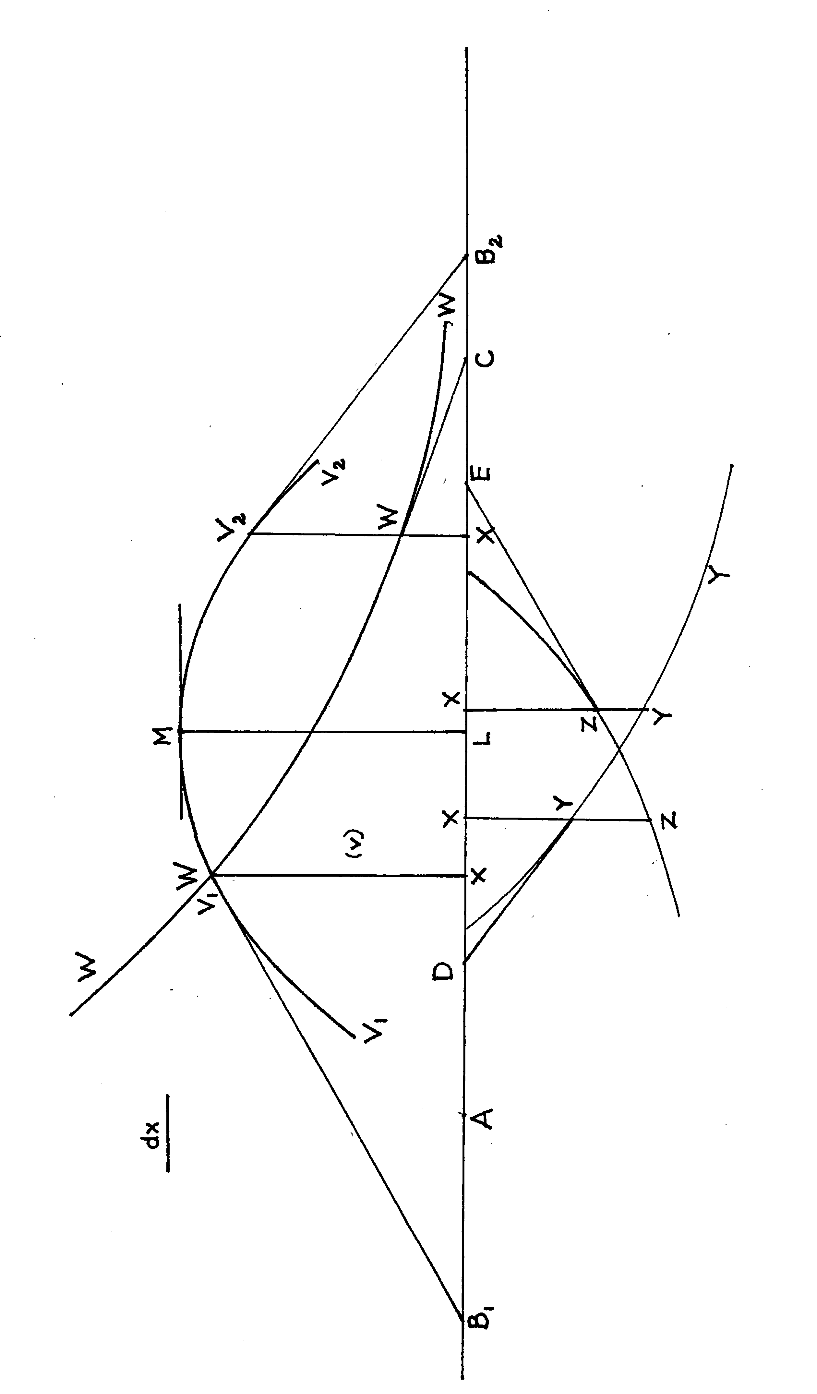
\includegraphics[width=.85\textwidth]{fig/Figure2}
    \caption{Leibniz's figure, slightly simplified}
    \label{newmeth1}
  \end{center}
\end{figure}
an axis $AX$, and several curves, such as $VV$, $WW$, $YY$, and $ZZ$;
let their ordinates normal [that is, perpendicular] to the axis be
$VX$, $WX$, $YX$, and $ZX$, let them be called $v$, $w$, $y$, and $z$,
respectively, and let $AX$, the abscissa cut off on the axis, be
called $x$.\marginnote{Note 2, p.~\pageref{cnm2}} Let the tangents be
$VB$, $WC$, $YD$, and $ZE$, meeting the axis at the points $B$, $C$,
$D$, and $E$, respectively.  Now let some arbitrary straight line be
called $dx$, and let the straight line which is to $dx$ as $v$ (or
$w$, or $y$, or $z$) is to $XB$ (or $XC$, or $XD$, or $XE$) be called
$dv$ (or $dw$, or $dy$, or $dz$) or the difference of the $v$'s
themselves (or of the $w$'s, $y$'s, or $z$'s
themselves).\marginnote{Note 3, p.~\pageref{cnm3}}\label{diffdef} If
we assume these things, the rules of the calculus will be as follows.


Let $a$ be a given constant quantity; then $da$ will be equal to 0,
and $d(ax)$ will be equal to $a\,dx$.\marginnote{Note 4,
  p.~\pageref{cnm4}} If $y = v$ (that is, if each ordinate of the
curve $YY$ is equal to the corresponding ordinate of the curve $VV$),
then $dy = dv$.  \newline Now for {\em Addition} and {\em
  Subtraction}: if
$$z-y+w+x = v,$$ then we shall have $$d(z-y+w+x) = dz-dy +dw + dx.$$ \newline
{\em Multiplication}:
$$d(xv) = x\,dv + v\,dx,$$ that is, setting $y = xv$,
$$dy = x\,dv + v\,dx;$$ for we are free to use either
a formula such as $xv$, or a letter as an abbreviation for it, such as
$y$. Note that in this calculus we treat $x$ and $dx$ in the same way
as $y$ and $dy$ or any other indeterminate letter together with its
differential.  Also note that we cannot always go backwards from a
differential equation, unless we are cautious; but let us not go into
that here. \newline Next, {\em Division}:\footnote{We have simplified
  Leibniz's rule.  Leibniz does not let the values of his ordinates
  change signs when a curve crosses the axis, and this makes his
  formula for the division rule more complicated.  Leibniz writes the
  division rule as follows:
$$d\left(\frac{v}{y}\right) = 
\frac{\pm v\,dy \mp y\,dv}{y^2}.$$ We will always take our ordinates
as negative when the curve is below the axis, following modern
conventions and avoiding Leibniz's ambiguous signs $\pm$ and $\mp$.}
$$d\left(\frac{v}{y}\right) \mbox{ or (setting $z = \frac{v}{y}$) }dz =
\frac{y\,dv - v\,dy }{y^2}.$$


As far as {\em Signs} are concerned, we should note that when we
substitute the differential of a letter for that letter we keep the
same sign, and we write $+dz$ in place of $+z$, and $-dz$ in place of
$-z$, as we can see from the addition and subtraction rule we laid
down above; but when it comes to the exegesis of values, that is, when
we consider the relation of $z$ to $x$, then it becomes clear whether
the value of $dz$ is positive or less than zero (negative): when this
happens, let us draw the tangent $ZE$ from the point $Z$ not towards
$A$, but in the opposite direction (to the right of $X$).\footnote{See
  Figure~\ref{incrdecr}.  At the first point where the ordinate is
  equal to $z$, that is, at the point on the left, $z_1$ is greater
  than $z$, and therefore $dz$, which is equal to $z_1 -z$, is
  positive.  At the second point where the ordinate is equal to $z$,
  that is, the point on the right, $z_1$ is less than $z$, and
  therefore $dz$ is negative.}
\begin{figure}[htp]
  \begin{center}
    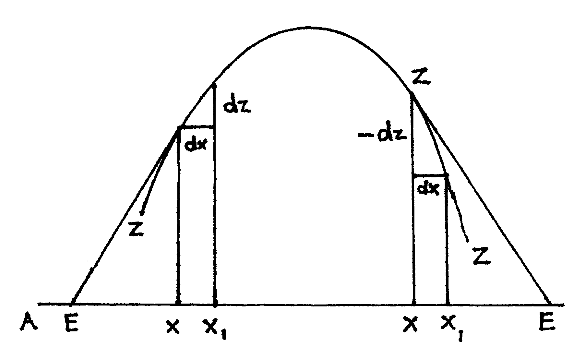
\includegraphics[width=.75\textwidth]{fig/Figure4}
    \caption{our figure, not Leibniz's}
    \label{incrdecr}
  \end{center}
\end{figure}
This happens when the ordinates $z$ decrease as the $x$'s increase.
And because the ordinates $v$ sometimes increase and sometimes
decrease, $dv$ will sometimes be a positive quantity and sometimes be
negative; in the former case we draw the tangent $V_1B_1$ towards $A$,
in the latter case in the opposite direction.
\label{dvzero}
But we do neither in the middle around $M$, for then the $v$'s
themselves neither increase nor decrease, but stand still, and
therefore $dv = 0$, and it does not matter whether the quantity is
positive or negative, for $+0 = -0$; and here $v$, that is, the
ordinate $LM$, is the {\em Greatest} ordinate (or if the convexity
turns towards the axis, the {\em Least}) and we draw the tangent to
the curve at $M$ neither towards $A$ (to the left of $X$), approaching
the axis there, nor in the opposite direction (to the right of $X$);
instead we draw it parallel to the axis. [See Figure~\ref{newmeth1} or
Figures~\ref{maxfig} and \ref{minfig}.]
\begin{figure}[htp]
  \begin{center}
    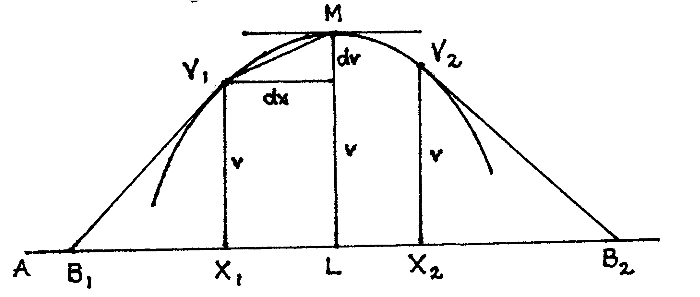
\includegraphics[width=.75\textwidth]{fig/Figure5}
    \caption{our figure, not Leibniz's}
    \label{maxfig}
  \end{center}
\end{figure}
\begin{figure}[htp]
  \begin{center}
    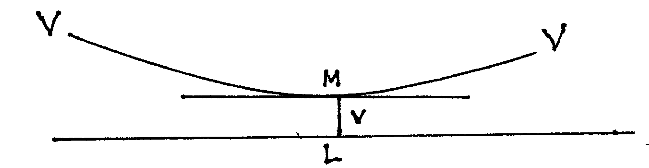
\includegraphics[width=.75\textwidth]{fig/Figure5A}
    \caption{our figure, not Leibniz's}
    \label{minfig}
  \end{center}
\end{figure}
If $dv$ is infinite with respect to $dx$, then the tangent is
perpendicular to the axis, that is, it is itself an
ordinate.\footnote{See Figure~\ref{verttang}.  Here, as $V_1$ becomes
  infinitely close to $V_p$, the ratio of $v_1 - v$ (that is, $dv$) to
  $x_1 - x$ (that is, $dx$), becomes infinite.}
\begin{figure}[htp]
  \begin{center}
    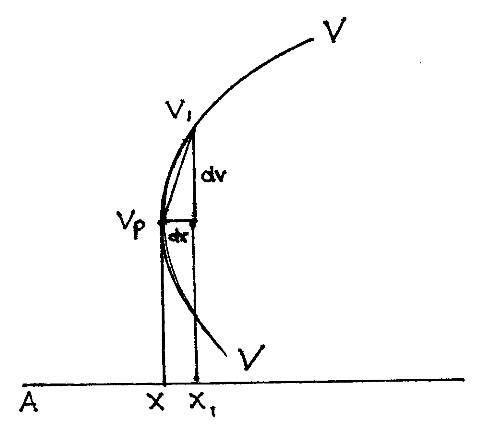
\includegraphics[width=.65\textwidth]{fig/Figure6}
    \caption{our figure, not Leibniz's}
    \label{verttang}
  \end{center}
\end{figure}
If $dv$ and $dx$ are equal, the tangent makes half a right angle with
the axis [see Figure~\ref{45deg}].
\begin{figure}[htp]
  \begin{center}
    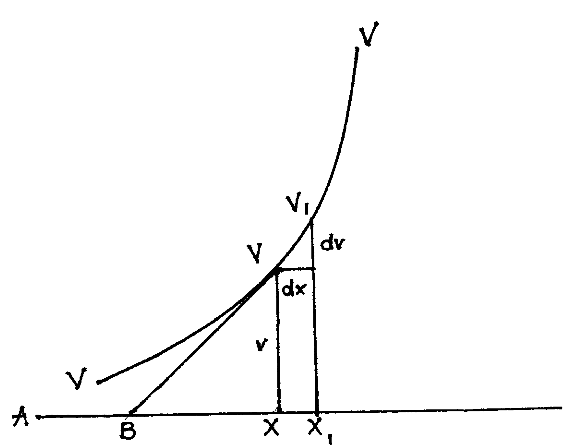
\includegraphics[width=.65\textwidth]{fig/Figure7}
    \caption{our figure, not Leibniz's}
    \label{45deg}
  \end{center}
\end{figure} If when the ordinates $v$ increase their increments or
differences $dv$ also increase (that is, if we suppose that the $dv$'s
are positive, then the $ddv$'s,\footnote{The modern notation for $ddv$
  is $d^2v$.}  the differences of their differences, are also
positive, and if negative, then negative), then the curve turns its
{\em convexity} toward the axis; in the opposite case [that is, where
the ordinates increase and their differences decrease], the curve
turns its {\em concavity} toward the axis.\footnote{See
  Figure~\ref{concavity}, page~\pageref{concavity}.  To say that ``the
  curve turns its convexity toward the axis," is to say that it bends
  away from the axis.  If it turns its concavity toward the
  axis, then it bends toward the axis.  Because we use signs in a
  different way from Leibniz's (see note~7, page~\pageref{cnm7}), the
  rule is even simpler for us: when $ddv$ is positive, the curve turns
  its convexity downward, that is, it bends upward; while if $ddv$ is
  negative, it turns its concavity downward, that is, it bends
  downward.}
\begin{figure}[htp]
  \begin{center}
    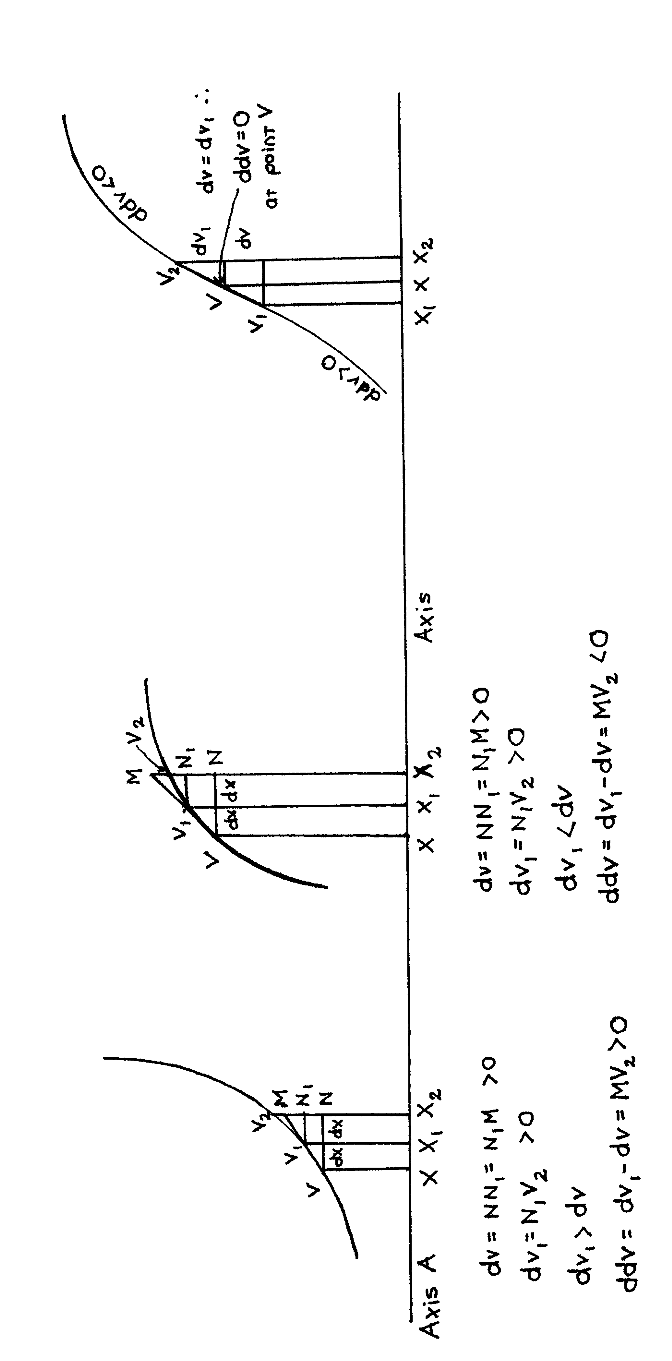
\includegraphics[width=.73\textwidth]{fig/Figure8}
    \caption{our figure, not Leibniz's}
    \label{concavity}
  \end{center}
\end{figure} But where there is a greatest or least increment, or
where the increments go from decreasing to increasing, or conversely,
there is an {\em inflection point}, and there is a change from
concavity to convexity, or conversely [see Figure~\ref{inflection},
page~\pageref{inflection}] provided that the ordinates do not also
change from increasing to decreasing at that point, or conversely, for
then the convexity or concavity would remain the same.
\begin{figure}[p]
  \begin{center}
    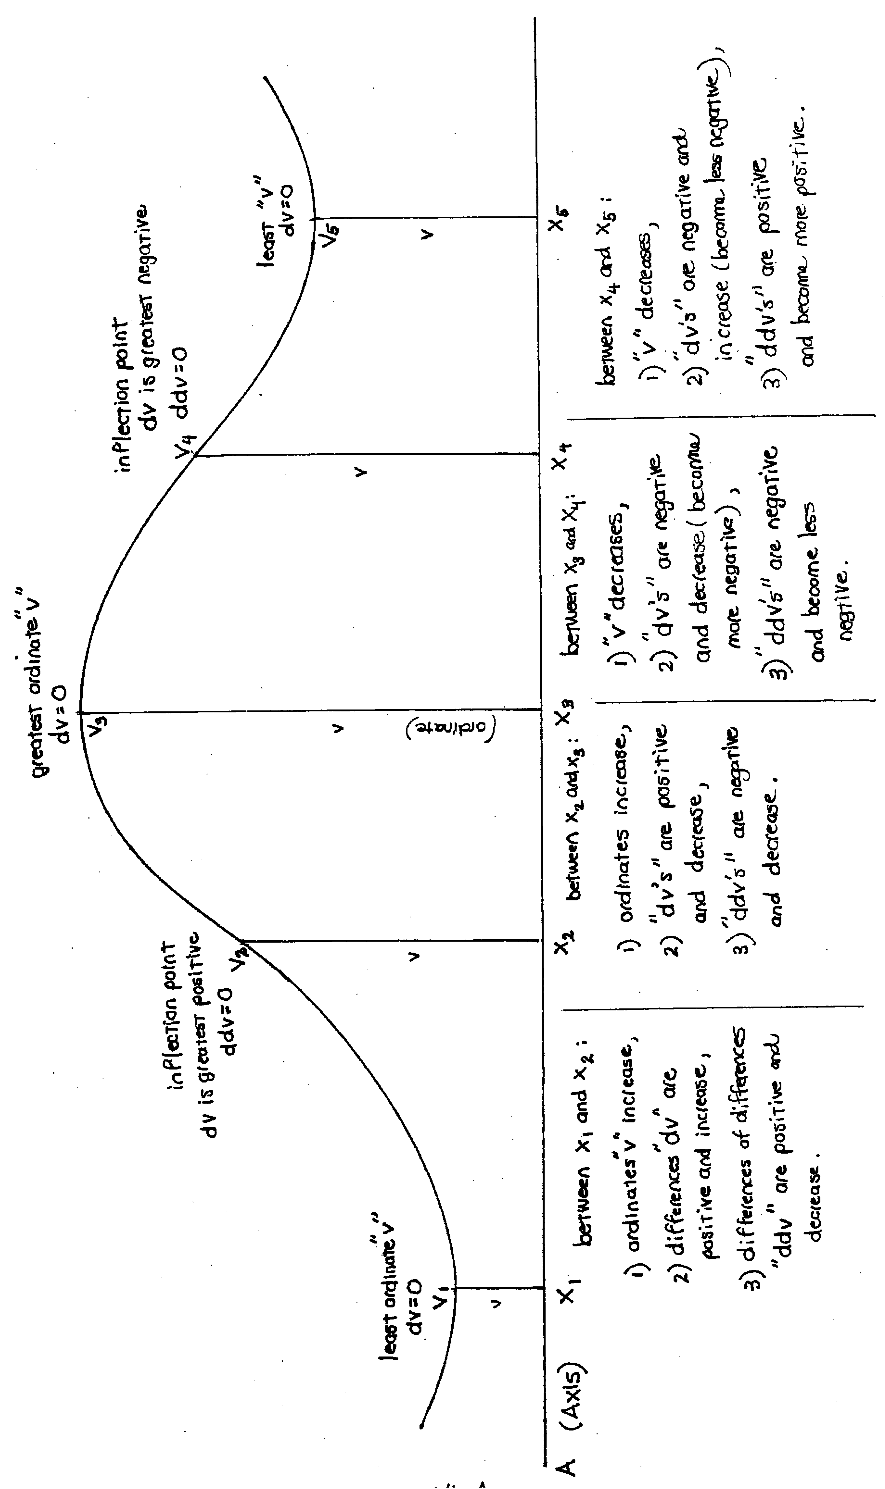
\includegraphics[width=.89\textwidth]{fig/Figure9}
    \caption{our figure, not Leibniz's}
    \label{inflection}
  \end{center}
\end{figure} But the increments cannot continue to increase or
decrease when the ordinates go from increasing to decreasing, or
conversely.  And so an inflection point occurs when neither $v$ nor
$dv$ is 0 but $ddv$ {\em is} 0.  It also follows that the problem of
finding an inflection point, unlike the problem of finding a greatest
ordinate, has not two, but three equal roots.\marginnote{Note 5,
  p.~\pageref{cnm5}} And all this of course depends on the correct use
of signs.\footnote{Here Leibniz includes a paragraph on signs, which
  we again can omit if we use signs in the modern way, letting
  ordinates become negative when a curve crosses the axis.  We have
  included the omitted paragraph in the accompanying notes after the
  fifth note (p.~\pageref{ompar}).}\label{ambsigns}

\vspace*{1ex} {\em Powers}: $$d(x^a) = ax^{(a-1)}\,dx;$$ for example,
$d(x^3) = 3x^2\,dx$.
$$d\left(\frac{1}{x^a}\right) = - \frac{a\,dx}{x^{(a+1)}};$$ e.g., if 
$$w =\frac{1}{x^3},$$ then 
$$dw = -\frac{3\,dx}{x^4}.$$

\vspace*{1ex} {\em Roots}:
$$d\sqrt[b]{x^a} = \frac{a}{b}\,dx\,\sqrt[b]{x^{(a-b)}}$$ (hence
$$d\sqrt[2]{y} = \frac{dy}{2\sqrt[2]{y}},$$ since in this case $a$ is 1, and
$b$ is 2; therefore
$$ \frac{a}{b}\sqrt[b]{x^{(a-b)}} \mbox{ is } \frac{1}{2}\sqrt[2]{y^{-1}};$$ now
$y^{-1}$ is the same as $\frac{1}{y}$, from the nature of the
exponents of the geometric progression, and $\sqrt[2]{\frac{1}{y}}$ is
$\frac{1}{\sqrt[2]{y}}$), and
$$d\left(\frac{1}{\sqrt[b]{x^a}}\right) = \frac{-a\,dx}{b\sqrt[b]{x^{(a+b)}}}.$$ But the rule
for a whole power would have sufficed to determine both fractions and
roots; for the power is a fraction when the exponent is negative, and
changes into a root when the exponent is a fraction.\marginnote{Note 6,
  p.~\pageref{cnm6}} But I chose to deduce such consequences myself,
rather than leave them for others to deduce, since they are quite
general and occur frequently, and since when something is so
inherently complicated we should try to find ways to make it
easier.\marginnote{Note 7, p.~\pageref{cnm7}}

Once we have learned this {\em Algorithm} (as I call it) of our
calculus (which I call the {\em differential calculus}), we can find
all other differential equations through the common calculus, and we
can obtain least and greatest lines, as well as tangents, without
needing to eliminate fractions and irrationals or other impediments,
as still had to be done when using the previously published methods.
Someone who is versed in these matters will easily be able to
demonstrate all these things if he considers the following point (one
that has not yet been given enough weight): that $dx$, $dy$, $dv$,
$dw$ and $dz$ themselves can be taken as proportional to the
differences (or momentary increments or decrements) of $x$, $y$, $v$,
$w$, and $z$ themselves (respectively).  We can use this to write down
the differential equation \label{nmdiffeq} for any given equation; we
simply substitute for any {\em term} (that is, for any of the parts
that are joined by addition or subtraction to make up the equation)
the differential quantity of that term; but for any other quantity
(which is not itself a term, but contributes to forming a term) we do
not directly use its differential quantity when forming the
differential quantity of the term to which it belongs; instead, we
follow the above algorithm.\marginnote{Note 8, p.~\pageref{cnm8}} In
contrast, the previously published methods\footnote{For an example of
  a previously published method for finding maxima and minima, see
  Pierre Fermat's ``On a method for the evaluation of maxima and
  minima," written in 1633 and translated on pages 223--225 of Dirk
  Struik's {\em A Source Book in Mathematics, 1200--1800} (Cambridge,
  1969). Fermat's $a$ corresponds to Leibniz's $x$, and Fermat's $e$
  corresponds to Leibniz's $dx$.  But for Fermat, the quantity $e$ is
  finite, not infinitely small.  In each problem Fermat therefore has
  to engage in special algebraic manipulations to eliminate $e$ from
  his final equation for the maxima or minima, while Leibniz has a
  general method that can always find a finite equation that does not
  involve $dx$. } do not have such a transition, since for the most
part they use a straight line such as $DX$ [see Figure~\ref{newmeth1}
or Figure~\ref{tanandord}],
\begin{figure}[htp]
  \begin{center}
    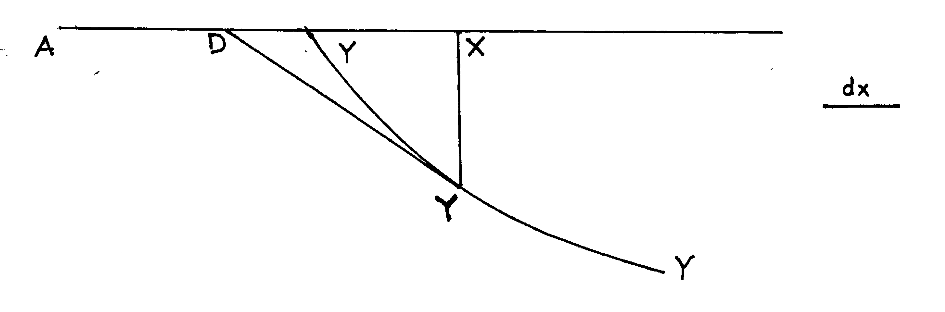
\includegraphics[width=.75\textwidth]{fig/Figure19}
    \caption{our figure, not Leibniz's}
    \label{tanandord}
  \end{center}
\end{figure} or another of the same kind, but not the line $dy$, which
is a fourth proportional for $DX$, $XY$, and $dx$, and this confuses
everything.  Because of this confusion they make it a rule that we
must first eliminate fractions and irrationals (those that the
indeterminates enter into).  It is clear that our method also extends
to transcendent lines---lines to which the algebraic calculus cannot
be applied, that is, lines which are of no definite
degree \label{trandef}\marginnote{Note 9, p.~\pageref{cnm9}}---and it
does this very generally, without any particular suppositions that
only sometimes apply, provided we hold in general that to find a {\em
  tangent} is to draw a straight line joining two points on a curve
that are an infinitely small distance apart\label{taninfcl}, or to
draw the side of a polygon with infinitely many angles (which is for
us equivalent to the {\em curve}).  And that infinitely small distance
can always be expressed through some known difference such as $dv$, or
through a relation to it, that is, through some known tangent.  For
example, if $y$ were a transcendent quantity, for instance the
ordinate of a cycloid, and it were to enter into the calculation by
means of which $z$, the ordinate of another curve, was to be
determined, and if we were looking for $dz$, or through it the tangent
of this latter curve, then we ought to determine $dz$ through $dy$,
since we know the tangent of the cycloid.  And similarly, if we were
to pretend that we did not know the tangent of the cycloid, we could
find it from a given property of the tangents of a
circle.\marginnote{Note 10, p.~\pageref{cnm10}}

\label{bnmex1} Let me give an example of the calculus.\footnote{Here
  we have omitted a parenthetical comment Leibniz makes on his
  notation: ``Note that I designate division here in the following
  way: $x\!:\!y$, which is the same thing as $x$ divid.\ by $y$ or
  $\frac{x}{y}$.''  We always denote $x$ divided by $y$ by
  $\frac{x}{y}.$} Let the {\em first} or given equation be
$$\frac{x}{y} + \frac{(a+bx)(c-x^2)}{(ex+fx^2)^2} + ax\sqrt{g^2 +y^2} +\frac{y^2}{\sqrt{h^2 + lx + mx^2}}= 0.$$
expressing the relation between $x$ and $y$, that is, between $AX$ and
$XY$ (see Figure~\ref{newmeth1} [or Figure~\ref{tanandord}]), where we
suppose that $a$, $b$, $c$, $e$, $f$, $g$, $h$, $l$, and $m$ are
given; we are looking for a way to draw, from a given point $Y$, the
line $YD$, which touches the curve.  In other words, we are looking
for the ratio of the straight line $DX$ to the given straight line
$XY$.  For the sake of brevity let us write $n$ in place of $a+bx$,
$p$ in place of $c-x^2$, $q$ in place of $ex + fx^2$, $r$ in place of
$g^2+y^2$, and $s$ in place of $h^2+lx +mx^2$.  Then we shall have:
$$\frac{x}{y} + \frac{np}{q^2} + ax\sqrt{r} + \frac{y^2}{\sqrt{s}} = 0,$$ which
is a {\em second} equation.  Now we know by our calculus that
$$d\left(\frac{x}{y}\right)$$ is
$$\frac{y\,dx - x\,dy}{y^2},$$ 
and similarly that
$$d\left(\frac{np}{q^2}\right)$$ is
$$ \frac{q(n\,dp + p\,dn) -2np\,dq}{q^3}$$ and
$$d(ax\sqrt{r})$$ is
$$ax\frac{dr}{2\sqrt{r}} + a\,dx\sqrt{r};$$ and 
$$d\left(\frac{y^2}{\sqrt{s}}\right)$$ is
$$  \frac{4ys\,dy   - y^2\,ds}{2s\sqrt{s}}.$$ All of these
differential quantities, from $d(\frac{x}{y})$ to
$d(\frac{y^2}{\sqrt{s}}),$ will together add up to 0, and this will
give us a {\em third} equation---the equation we get when we
substitute for the terms of the second equation the quantities of
their differentials.\footnote{To be explicit, the third equation is:
$$\frac{y\,dx - x\,dy}{y^2} + \frac{q(n\,dp + p\,dn) -2np\,dq}{q^3} + ax\frac{dr}{2\sqrt{r}} + a\,dx\sqrt{r} + \frac{4ys\,dy   - y^2\,ds}{2s\sqrt{s}} = 0.$$}  Now $dn$ is $b\,dx$, and $dp$ is
$-2x\,dx$, and $dq$ is $e\,dx + 2fx\,dx$, and $dr$ is $2y\,dy$, and
$ds$ is $l\,dx + 2mx\,dx$.  Substituting these values into the third
equation we shall get a {\em fourth} equation, where the only
remaining differential quantities---$dx$ and $dy$---are always
unbound\footnote{That is, they are never contained in parentheses or
  under a radical.}  and never in a denominator, and each term has
either a $dx$ or a $dy$.  Thus the law of homogeneity\marginnote{Note
  11, p.~\pageref{cnm11}} is always observed as far as these two
quantities are concerned, however complicated the calculation may be.
From here we can always obtain the value of $\frac{dx}{dy}$ (the ratio
of $dx$ to $dy$ or of the line $DX$ we are looking for to the given
line $XY$).  According to our calculation\footnote{Leibniz is skipping
  very many algebraic steps here.} (changing the fourth equation into
a Proportion) this ratio will be the same as the ratio of
$$ \frac{x}{y^2} - \frac{axy}{\sqrt{r}}  - \frac{2y}{\sqrt{s}}$$ to
$$\frac{1}{y} - \frac{2np(e + 2fx)}{q^3} + \frac{-2nx + pb}{q^2}
+ a\sqrt{r} - \frac{y^2(l + 2mx)}{2s\sqrt{s}}.$$ But $x$ and $y$ are
given, because the point $Y$ is given.  The above mentioned values of
the letters $n$, $p$, $q$, $r$, and $s$ are also given through $x$ and
$y$.  Therefore we shall have what we are looking for.  I have
included this rather complicated example only to help show how to use
the above rules in a still more difficult calculation.  Let me now
give some easier examples that show how to use these
rules.\label{enmex1}

\label{bnmex2} Suppose we are given two points $C$ and $E$
(Figure~\ref{leasttime}),
\begin{figure}[htp]
  \begin{center}
    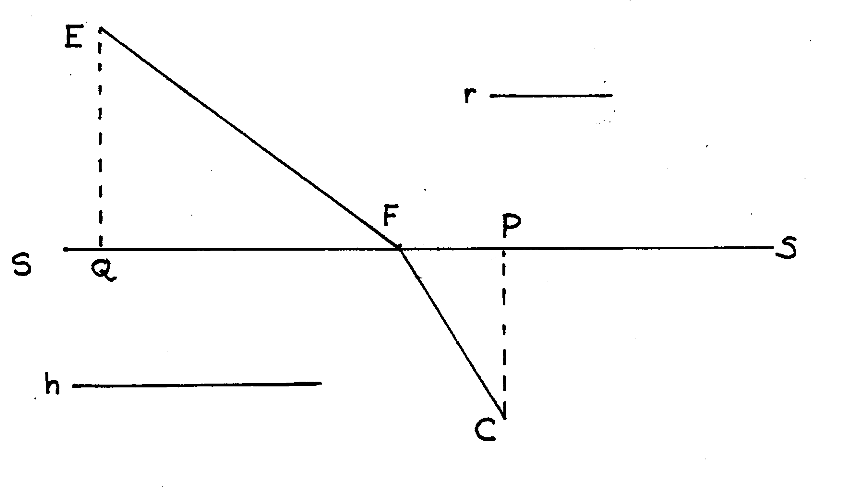
\includegraphics[width=.75\textwidth]{fig/Figure21}
    \caption{Leibniz's figure}
    \label{leasttime}
  \end{center}
\end{figure} along with a straight line $SS$ in the same plane; we are
looking for a point $F$ such that when we connect the lines $CF$ and
$EF$, then the sum of the rectangles $CF$ times a given line $h$ and
$EF$ times a given line $r$ is as small as possible.  That is, if $SS$
is a line separating two media, and $h$ represents the density of a
medium (such as water) on the side where $C$ is, while $r$ represents
the density of a medium (such as air) on the side where $E$ is, then
we are looking for a point $F$ such that the path from $C$ to $E$
through $F$ is the easiest possible one.\marginnote{Note 12,
  p.~\pageref{cnm12}} Let us suppose that all the possible sums of
such rectangles, or all the possible difficulties of the paths, are
represented by the lines $KV$ (Figure~\ref{leasttime2}),
\begin{figure}[htp]
  \begin{center}
    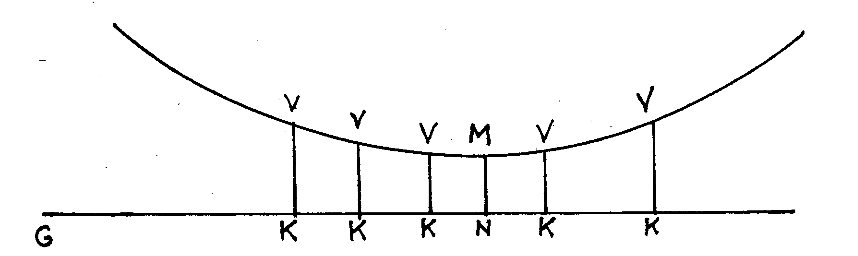
\includegraphics[width=.75\textwidth]{fig/Figure22}
    \caption{part of Leibniz's Figure~\ref{newmeth1}, modified}
    \label{leasttime2}
  \end{center}
\end{figure}
that is, by the ordinates of the curve $VV$ that are normal to the
straight line $GK$.\marginnote{Note 13, p.~\pageref{cnm13}} We shall
call these ordinates $\omega$; we are looking for the least ordinate,
$NM$.  Because the points $C$ and $E$ [in Figure~\ref{leasttime}] are
given, their perpendiculars to $SS$, namely $CP$ (which we shall call
$c$) and $EQ$ (which we shall call $e$), will also be given, along
with $PQ$ (which we shall call $p$).  And we shall call $QF$, which is
equal to $GN$ [in Figure~\ref{leasttime2}], $x$, and $CF$, $f$, and
$EF$, $g$.  Then $FP$ will become $p-x$, and\marginnote{Note 14,
  p.~\pageref{cnm14}}
$$f  = \sqrt{c^2+p^2-2px + x^2}\;\mbox{ or, abbreviating, }\sqrt{l},$$
and
$$g =  \sqrt{e^2+x^2}\;\mbox{ or, abbreviating, }\sqrt{m}.$$ We
therefore have
$$\omega =  h\sqrt{l} + r\sqrt{m},
$$ and the differential of this
equation (setting $d\omega$ to be 0 since $\omega$ is the least
ordinate) is 0 and equal to
$$\frac{h\,dl}{2\sqrt{l}} + \frac{r\,dm}{2\sqrt{m}},$$ through the rules we have
given for our calculus;\marginnote{Note 15, p.~\pageref{cnm15}}[-0.75ex] now
$dl$ is $-2dx(p-x),$\marginnote{Note 16, p.~\pageref{cnm16}}[1ex] and $dm$
is $2x\,dx$, and therefore:
$$\frac{h(p-x)}{f} = \frac{rx}{g}. $$ Now\marginnote{Note 17, p.~\pageref{cnm17}} if we apply this
to dioptrics, and if we suppose that $f$ and $g$, or $CF$ and $EF$,
are equal (for the refraction at the point $F$ remains the same,
whatever length we choose for the straight line $CF$), then
$$h(p-x) = rx,$$ that is,
$$h\!:\!r::x\!:\!p-x,$$ or $h$ is to $r$ as $QF$ is to $FP$.  In other words,
the sines $FP$ and $QF$ of the angles of refraction will be
reciprocally as $r$ and $h$, the densities of the media in which the
incidence and refraction occur.\marginnote{Note 18, p.~\pageref{cnm18}}
However, this density should not be understood in relation to
ourselves, but in relation to the resistance that the rays of light
meet.  And thus we have a demonstration of the calculus, which we
published elsewhere in these very {\em Acts}, when we were setting out
a general foundation for optics, catoptrics and
dioptrics;\marginnote{Note 19, p.~\pageref{cnm19}} for other extremely
learned men have pursued in very roundabout ways things that someone
skilled in our calculus will henceforth be able to produce in three
lines.\label{enmex2} \label{bnmex3} I will show this with yet another
example.  Let the curve 133 (Figure~\ref{locus})
\begin{figure}[htp]
  \begin{center}
    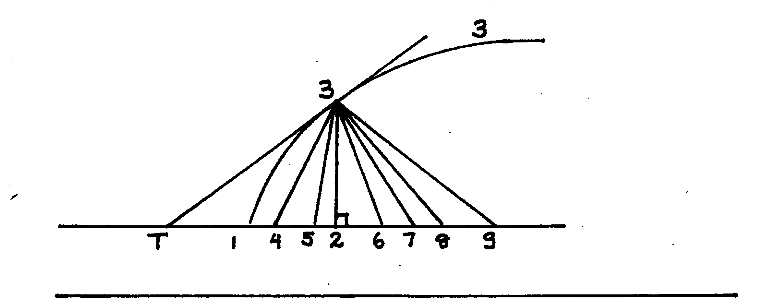
\includegraphics[width=\textwidth]{fig/Figure24}
    \caption{Leibniz's figure}
    \label{locus}
  \end{center}
\end{figure} be of such a nature that if from any point on it, such as
3, we draw six lines, 34, 35, 36, 37, 38, and 39 to six fixed points
placed on the axis, 4, 5, 6, 7, 8, and 9, then these six lines taken
together are equal to a given straight line $g$.  Let $T$14526789 be
the axis, and let $12$ be an abscissa and $23$ be an ordinate.  We are
looking for the tangent $3T$.  I say that $T2$ will be to $23$
as\marginnote{Note 20, p.~\pageref{cnm20}}
$$\frac{23}{34} + \frac{23}{35} +\frac{23}{36} + \frac{23}{37} + \frac{23}{38}
+\frac{23}{39}$$ is to
$$-\frac{24}{34} - \frac{25}{35} +\frac{26}{36} +\frac{27}{37} + \frac{28}{38}
+ \frac{29}{39}.$$ The same rule will apply, only with more terms, if we
should suppose there are not six, but ten or more points; all such problems would be
extremely tedious and sometimes even impossible to calculate by eliminating
all the irrationals and using the published methods of tangents.  Likewise, if 
the plane or solid rectangles constructed by using all possible pairs or
triples of those straight lines should be equal to a given quantity, the problem would again be extemely tedious or impossible using the published methods.\label{enmex3}  \marginnote{Note 21, p.~\pageref{cnm21}}  But in all these cases, and in much more complicated ones, our method is
extraordinarily easy, much more so than we might have expected.  And these are
only the beginnings of a certain much more elevated geometry, which also
pertains to some of the most difficult and beautiful problems of mixed
mathematics, problems which no one will be able to deal with easily by
proceeding blindly without our differential calculus or something like it.  \label{begdeb} As
an appendix, let me add the solution to a problem proposed by {\em De Beaune}
to {\em Descartes}.  Descartes tried to solve it in Vol.\ 3 of his {\em
Letters}, but failed.  Here is the problem: to find a line $WW$ (Figure~\ref{newmeth1} or Figure~\ref{debeaune})
\begin{figure}[htp]
\begin{center}
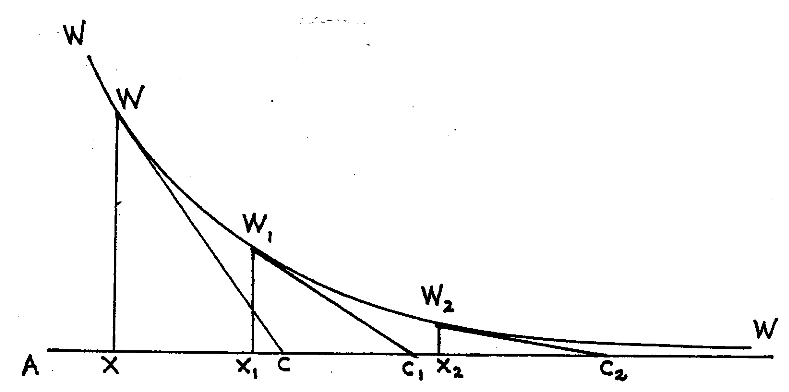
\includegraphics[width=.8\textwidth]{fig/Figure26}
\caption{our figure, not Leibniz's}
\label{debeaune}
\end{center}
\end{figure} 
  of
such a nature that if a tangent $WC$ is drawn to the axis, then $XC$ is always
equal to the same constant straight line $a$.  Now $XW$ (or $w$) is to $XC$
(or $a$) as $dw$ is to $dx$; therefore if $dx$ (which may be taken
arbitrarily) is taken to be constant or always the same (say it is $b$), that
is, if the $x$'s or $AX$'s increase uniformly, then $w$ will be equal to
$\frac{a}{b}dw$.  These $w$'s will thus themselves be proportional to their own
increments or differences; but that is to say that if the $x$'s are in an arithmetic
progression, then the $w$'s will be in a geometric progression.\marginnote{Note 22, p.~\pageref{cnm22}}  In other words,
if the $w$'s are numbers, then the $x$'s will be logarithms.  $WW$ is therefore
a logarithmic line.\label{enddeb}
\label{endnm}

\newpage



\section*{Notes on Leibniz's ``A New Method"}
%\addcontentsline{toc}{section}{\protect\numberline{3}{Notes on
\acl{Notes on Leibniz's ``A New Method"}

Leibniz published this paper in the journal {\em Acta Eruditorum}, {\em Acts of the Erudite}, in October of 1684.  The paper is written in Latin, and we have translated it from a text published in C.\ I.\ Gerhardt's edition of Leibniz's mathematical writings, Volume V, pages 220--226.  We have slightly modernized his notation throughout the paper.

\subsection*{Note 1}
\label{cnm1}

It may be helpful to say in general terms what Leibniz is doing in this paper.  He is, as the title says, introducing a new mathematical method.  The method is used for two basic kinds of problems: 
\begin{enumerate} 
\item Finding greatests and leasts.  In its most general terms, the problem is to find the greatest or least possible values for a variable quantity.  A simple example is finding the greatest ordinate for an ellipse with a given diameter.  See Figure~\ref{glord}.  
\begin{figure}[htp]
\begin{center}
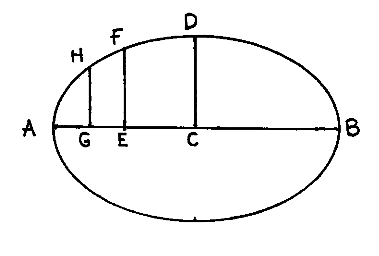
\includegraphics[width=0.5\textwidth]{fig/Figure1}
\vspace{-20pt}
\caption{}
\label{glord}
\end{center}
\end{figure}


There $ADB$ is an ellipse whose major axis is $AB$ and whose center is $C$.  Then the greatest ordinate is of course the ordinate $DC$ meeting the axis at the center, $C$, of the ellipse.  There is no need for a new method here. But Leibniz's method will give us a way to find the greatest and least ordinates not just for an ellipse or other conic section, but for any {\em  curve} whose Cartesian equation we have.   For example,  Leibniz's method can help us find the greatest ordinate $CF$ and the least ordinate $BE$ of the curve $ABCD$. (See Figure~\ref{glord2})
\begin{figure}[htp]
\begin{center}
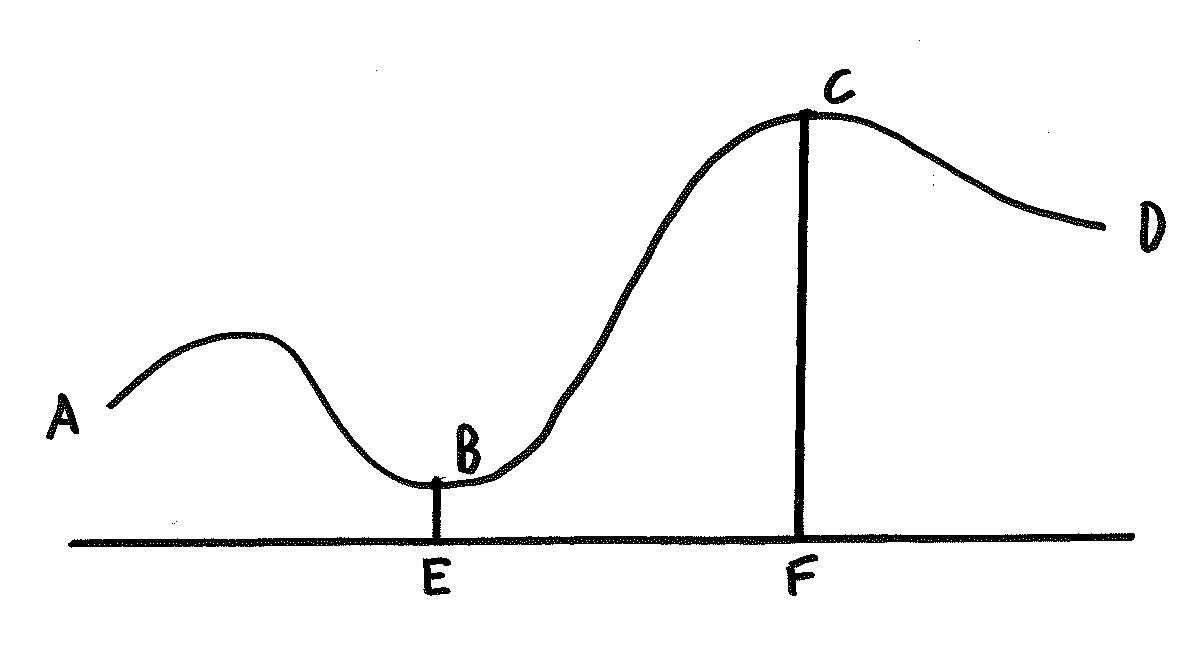
\includegraphics[width=0.6\textwidth]{fig/Figure1A}
\vspace{-20pt}
\caption{}
\label{glord2}
\end{center}
\end{figure}
 

Even if the Cartesian equation includes fractions and irrational quantities like square roots, the method still works.

\item Finding tangents to curves.  Here again the method is not restricted to conic sections or other simple kinds of curves, but can be used to find tangents at any point on any curve whose Cartesian equation we have.
\end{enumerate}

As the title also indicates, the method for solving these two kinds of problems depends on a ``singular calculus."   By a calculus, Leibniz seems to mean a way of calculating, that is, a system of symbols and a set of rules for using them.  He introduces in this paper one new symbol, $d$, and gives rules for using it together with ordinary algebra.   There are six rules, each showing how $d$ relates to one of six basic algebraic operations: addition, subtraction, multiplication, division, taking powers, and taking roots.  This new symbol and these new rules are the key to finding greatests, leasts, and tangents.  

After introducing the new calculus, Leibniz works through four examples in some detail.  He shows how to find the tangents to particular curves (pages~\pageref{bnmex1}--\pageref{enmex1} and page~\pageref{begdeb}), how to find the least value of a quantity (pages~\pageref{bnmex2}--\pageref{enmex2}), and how to find a curve whose tangents have a given property (pages~\pageref{bnmex3}--\pageref{enmex3}).


\subsection*{Note 2}
\label{cnm2}

Note that in Leibniz's Figure~\ref{newmeth1} (Figure~\ref{newmeth1A}, below)
\begin{figure}[htp]
\begin{center}
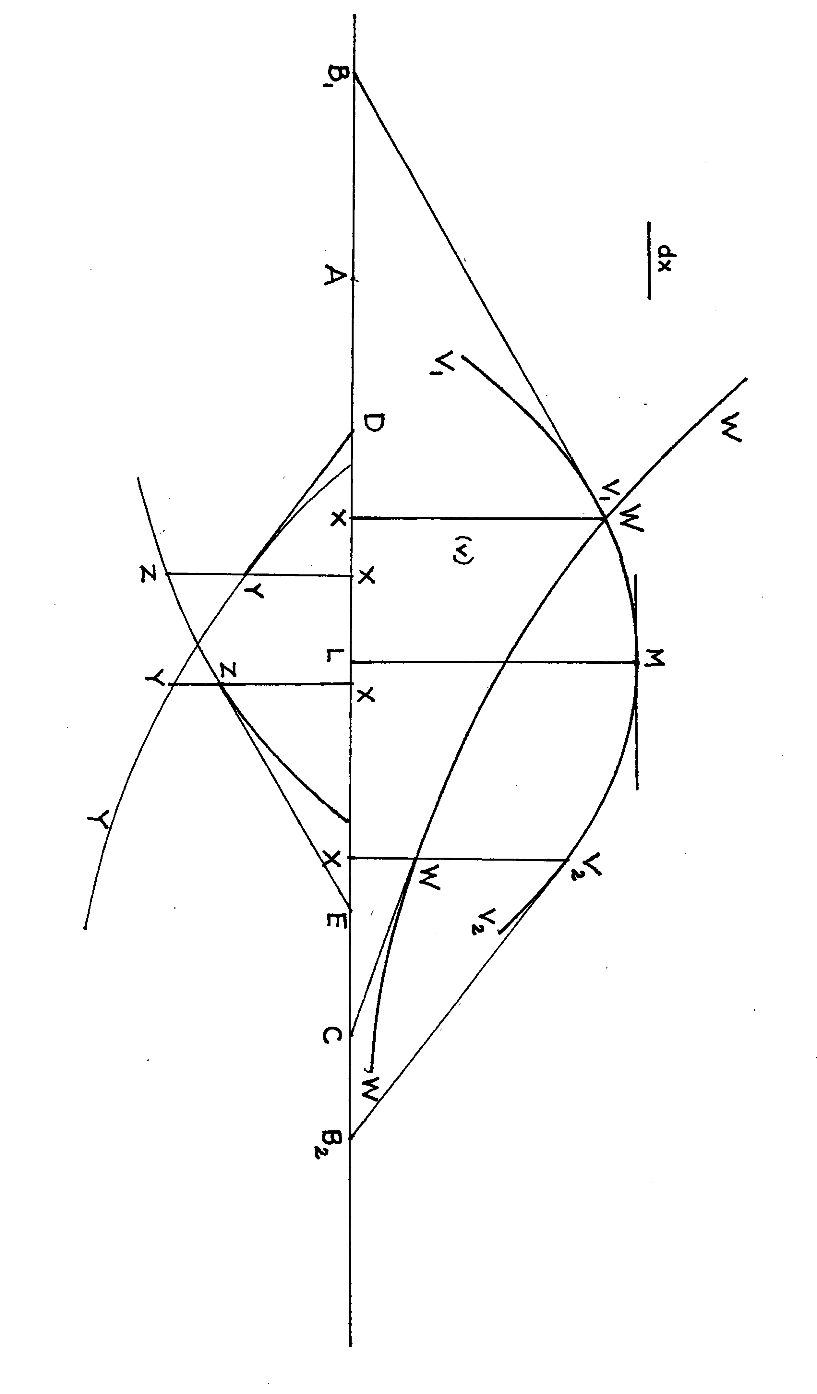
\includegraphics[width=.85\textwidth]{fig/Figure2A}
\caption{Leibniz's figure, slightly simplified}
\label{newmeth1A}
\end{center}
\end{figure}
 there are two lines $VX$, namely $V_1X$ and $V_2X$, and likewise two lines $WX$, two lines $YX$, and two lines $ZX$.  By drawing each of these lines twice in the diagram, Leibniz is suggesting that they should be understood as {\em variable} lines. (Leibniz does not use the term {\em variable} in this paper, but he introduces it in later writings.\footnote{See the papers ``On the line formed by infinitely many lines drawn ordinatewise which concur with each other and touch it," published in April of 1692 in the {\em Acts of the Erudite}, and ``A new application of the differential calculus and its use for finding multiple constructions of lines from a given condition on their tangents," published in July of 1694 in the same journal.  The former is on pages 266--9 in Volume V of Gerhardt's edition of Leibniz's mathematical works, and the latter paper is on pages 301--6 of the same volume.})  In other words, the line $VX$ should be understood not simply as one fixed line, but as a line that could be any of the infinitely many ordinates to the curve $VV$.



\subsection*{Note 3}
\label{cnm3}

To understand what Leibniz means by $dv$, consider Figure~\ref{dv}.  
\begin{figure}[htp]
\begin{center}
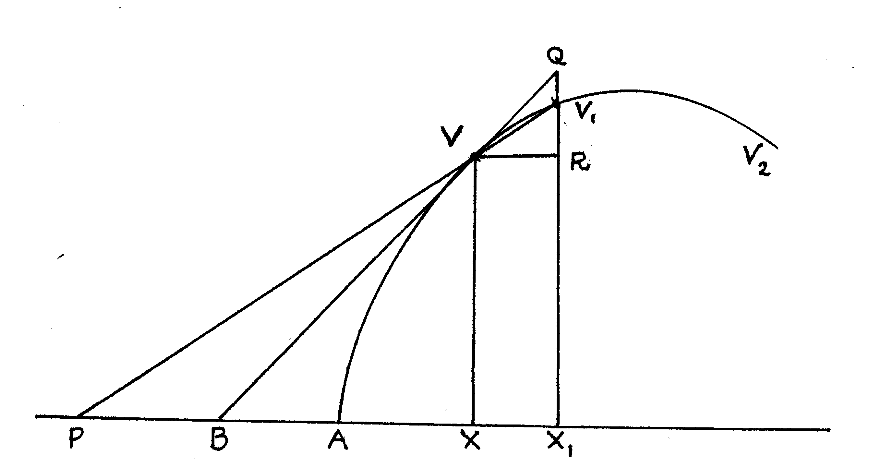
\includegraphics[width=.75\textwidth]{fig/Figure3}
\caption{}
\label{dv}
\vspace{-10pt}
\end{center}
\end{figure}
There we have drawn the curve $V_1V_2$ with ordinates $v$ from
Figure~\ref{newmeth1A}, along with the axis $AX$, but without all the
other curves.  We have relabeled one of the two points $X$, naming it
$X_1$.  We have added a point $V$ on the curve to the left of $V_1$,
drawn an ordinate $VX$ and a tangent $VB$, and connected $V_1V$ and
extended it to meet the axis $AX$ at $P$.  We have drawn a
perpendicular $VR$ from $V$ to the ordinate $V_1X_1$, and extended the
tangent $BV$ and the ordinate $V_1X_1$ to meet at $Q$.  Let $AX$ and
$AX_1$ be called $x$, and $x_1$, respectively, and let $VX$ and
$V_1X_1$ be called $v$, and $v_1$, respectively.  Now $dx$ is an
arbitrary line, and therefore we may take $dx$ as the difference of
$x$ and $x_1$:
$$dx = x_1 -x = AX_1 - AX = XX_1 = VR.$$

Leibniz suggests here we think about $dv$ in at least two different ways:
\begin{enumerate}
\item As a fourth term in a proportion:
$$dv\!:\!dx :: v \!:\! XB,$$ 
that is
$$dv\!:\!dx :: VX \!:\! XB.$$
Because triangle $VRQ$ is similar to triangle $BXV$,
$$ VX \!:\! XB :: QR\!:\!RV.$$
If we put these last two proportions together, it follows that
$$dv\!:\!dx :: QR\!:\!RV.$$
But $dx = RV$, and therefore, according to the first way of thinking about $dv$, $dv = QR$.

\item As the ``difference of the $v$'s":
$$dv  = v_1 - v = V_1X_1 - VX = V_1R.$$
\end{enumerate}

Now in general these two ways of thinking about $dv$ are not
compatible, as $QR$ is not equal to $V_1R$.  But if $V_1$ is {\em
  infinitely} close to $V$, then we may suppose that the line through
$V$ and $V_1$ {\em is} the tangent\footnote{Leibniz makes this
  explicit on page~\pageref{taninfcl} of this paper.} $VB$ and we may
take $QR$ to be equal to $V_1R$.  Thus the two ways of thinking about
$dv$ are compatible when we take the arbitrary line $dx$ as an
infinitely small line, so that the points $V$ and $V_1$ are infinitely
close.  In this case the ordinate $v_1$ only differs by an infinitely
small amount from the ordinate $v$, and therefore in a certain sense
these ordinates are two copies of the same ordinate $v$.  The
difference of $v_1$ and $v$ is thus not a difference of two different
$v$'s, but a {\em difference of $v$ itself}.  Because the ordinate $v$
is variable, the difference $dv$ is also variable, and for the
different ordinates $v$ there are different differences, all
represented by the symbol $dv$.
\begin{figure}[h]
\begin{center}
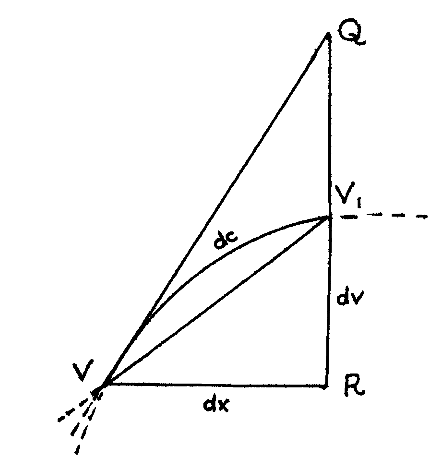
\includegraphics[width=.5\textwidth]{fig/Figure3A}
\caption{Magnification of Figure~\ref{dv} between $V$ and $V_1$.}
\label{chartrifig}
\vspace{-10pt}
\end{center}
\end{figure}

As Leibniz points out on page~\pageref{taninfcl}, taking two points as
infinitely close on a curve amounts to treating it as equivalent to a
polygon with infinitely many infinitely small sides: when the point
$V_1$ is infinitely close to the point $V$, the straight line $V_1V$
is one of the infinitely small sides of the polygon.
% Salviati in Galileo's {\em Two New Sciences}\footnote{In {\em
% Opere}, Favaro edition, Volume VIII, page~71; page~33 in Drake's
% translation.} treats the circle in a similar way.

Finally, we should note that in a number of later writings Leibniz
calls the infinitely small triangle $VRV_1$ the {\em characteristic
  triangle}\label{chartri} for the curve $VV_1$.  (See
Figure~\ref{chartrifig}.) It is an infinitely small right triangle
whose legs, $VR$ and $V_1R$, are equal to $dx$ and $dv$, respectively.
The hypotenuse of the characteristic triangle is the chord $VV_1$.
Because the points $V$ and $V_1$ are infinitely close, the chord
$VV_1$ coincides with the arc $VV_1$.  If we denote the length of arc
$AV$ by $c$, then the arc $VV_1$ will be equal to $dc$, the difference
of the $c$'s:
\begin{eqnarray*}
VV_1 & = &\mbox{arc }AV_1 - \mbox{arc }AV\\
& = & c_1 - c\\
& = & dc.
\end{eqnarray*}
According to Proposition I~47 in Euclid's {\em Elements}, the square
on $VV_1$ is equal to the square on $V_1R$ and the square on $VR$,
that is
$$dc^2 = dx^2 + dv^2.$$


% To understand what Leibniz may mean by calling this triangle
% ``characteristic," recall that for him the ``general characteristic"
% is the science by which we find suitable symbols (or characters) for
% thoughts.  By means of this science our thoughts are ``painted and
% fixed, and contracted and put in order."\footnote{See pages 9--10 of
% ``An Approach to the Arithmetic of Infinites," and Note~7.}  In our
% Figure~\ref{dv}, the triangle $VRV_1$ is a concise picture that
% leads us to think about all the differences of the curve and their
% relations to each other.  It is thus itself a kind of symbol or
% character, and therefore it may reasonably be called characteristic.
% Moreover, thinking about this triangle, we are led to the symbols
% and rules of Leibniz's calculus, and the triangle is thus
% characteristic not only because it is itself a kind of symbol
% leading us to think about the curve, but also because it directs our
% thought to develop a whole new system of symbols.  We will see that
% the characteristic triangle is central to Leibniz's way of thinking
% about the calculus and to its applications.

\subsection*{Note 4}
\label{cnm4}

In this sentence Leibniz introduces two rules for dealing with
differences involving constant quantities $a$.  Unlike the later
rules, he does not name these.  We will call the rule that $da =0$ the
{\em constant rule} and the rule that $d(ax) = a\,dx$ the {\em
  constant multiple rule}.  For the sake of brevity we sometimes refer
to these two rules together as the ``constant rules."

Leibniz does not demonstrate this or any of the other rules he gives.
We will give demonstrations of all the rules in the seventh note,
below.

\subsection*{Note 5}
\label{cnm5}

See Figure~\ref{maxinf}. 
\begin{figure}[ht]
\begin{center}
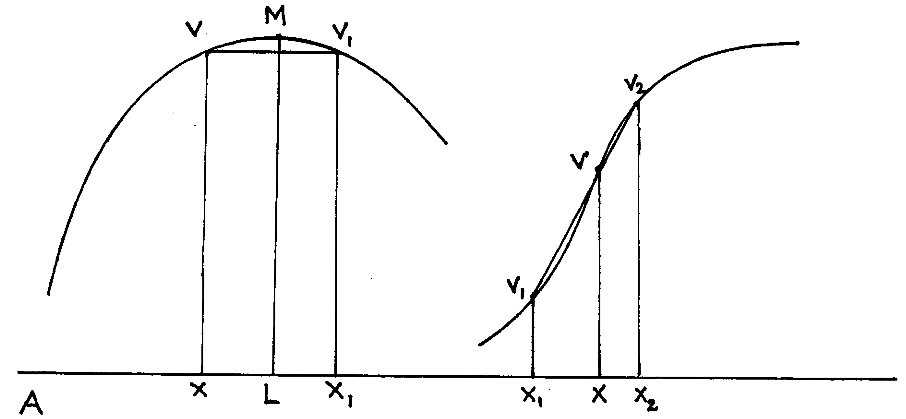
\includegraphics[width=\textwidth]{fig/Figure10}
\caption{}
\label{maxinf}
\vspace{-10pt}
\end{center}
\end{figure} To find a greatest ordinate, we have to find a horizontal
line that meets the curve at two infinitely close points $V$ and
$V_1$.  Finding these two points by algebra would involve finding two
roots (that is, solutions) of one equation (the details are not
important here).  These two roots become closer as $V$ becomes closer
to $V_1$, and when $V$ and $V_1$ become infinitely close, the two
roots become equal and the points $V$ and $V_1$ coincide at a point
$M$ where there is a greatest ordinate $LM$.  To find an inflection
point, we have to find a line that meets the curve at three infinitely
close points, $V$, $V_1$, and $V_2$.  Finding these points by algebra
would involve finding three roots to one equation, roots which would
become equal as $V$, $V_1$, and $V_2$ become infinitely close to one
another.

\subsection*{Leibniz's paragraph on ambiguous signs (page~\pageref{ambsigns})}
\label{ompar}

Here is the paragraph we have omitted from the main text.
\begin{quote}
  But sometimes we must use {\em ambiguous Signs}, as we just did in
  the {\em Division} rule, before we know how to explicate them.  And
  indeed, if when the $x$'s are increasing, the $\frac{v}{y}$'s are
  increasing (decreasing), the ambiguous signs in $d\,\frac{v}{y}$ or
$$\frac{\pm v\,dy \mp y\,dv}{yy}$$ should be explicated so that this fraction
becomes a positive (negative) quantity.  And $\mp$ signifies the
opposite of $\pm$, so that if the latter is $+$, then the former is
$-$, or conversely.  Many ambiguities can occur in the same
calculation, and I distinguish them by parentheses; for example, if
$w$ were
$$=\frac{v}{y} + \frac{y}{z} +\frac{x}{v},$$ then $dw$ would be
$$= \frac{\pm v\,dy \mp y\,dv}{yy} + \frac{\,(\pm)\, y\,dz \,(\mp)\,
  z\,dy}{zz} + \frac{\,(\!(\pm)\!)\, x\,dv \,(\!(\mp)\!)\,
  v\,dx}{vv};$$ otherwise the ambiguities from different sources might
be confused.  Note here that an ambiguous sign when multiplied by
itself gives $+$, when multiplied by its opposite gives $-$, and when
multiplied by another ambiguous sign forms a new ambiguity dependent
on both.
\end{quote}





\subsection*{Note 6}
\label{cnm6}

If Leibniz had simply given us the rule for powers,
$$d(x^a) = ax^{(a-1)}\,dx,$$
where $a$ could be any fraction, positive or negative, then the rule
for fractions whose denominators are powers and the rule for roots
would follow as special cases of this power rule.  For if we want to
find
$$d\left(\frac{1}{x^a}\right),$$
then we note that 
$$\frac{1}{x^a} = x^{-a},$$
and apply the power rule, substituting $-a$ for $a$, and simplify:
\begin{eqnarray*}
d(x^{-a}) & = & -ax^{((-a)-1)}\,dx \\
& = & -ax^{-(a+1)}\,dx\\
& = & -\frac{a\,dx}{x^{(a+1)}}
\end{eqnarray*}
This last expression is the one given by Leibniz's rule.

Likewise, if we want to find
$$d\sqrt[b]{x^a},$$
then we note that
$$\sqrt[b]{x^a} = x^{(\frac{a}{b})},$$
and apply the power rule, substituting $\frac{a}{b}$ for $a$, and simplify:
\setlength{\jot}{1.5ex}
\begin{eqnarray*}
d(x^{(\frac{a}{b})}) & = & \frac{a}{b}x^{((\frac{a}{b})-1)}\,dx \\
& = & \frac{a}{b}x^{\frac{1}{b}(a-b)}\,dx\\
& = & \frac{a}{b}\sqrt[b]{x^{(a-b)}}\,dx
\end{eqnarray*}
\setlength{\jot}{\oldjot}
This last expression is the one given by Leibniz's rule for roots.

\subsection*{Note 7}
\label{cnm7}

This long note contains seven parts:
\begin{enumerate}
\itemsep0em
\item{Examples of finding differences,}
\item{Problems about finding differences,}
\item{Demonstrations of Leibniz's rules,}
\item{Examples of finding greatest and least ordinates,}
\item{Problems about finding greatest and least ordinates,}
\item{Examples of finding tangents, and}
\item{Problems about finding tangents.}
\end{enumerate}

\subsubsection*{1. Examples of finding differences}

We can now use Leibniz's rules to find the differences of any algebraic expression involving $x$.  Here are some examples.
\begin{enumerate}
\item \label{ex1} Let $v= x^2 + 2.$  (See Figure~\ref{parex}.)
\begin{figure}[htp]
\begin{center}
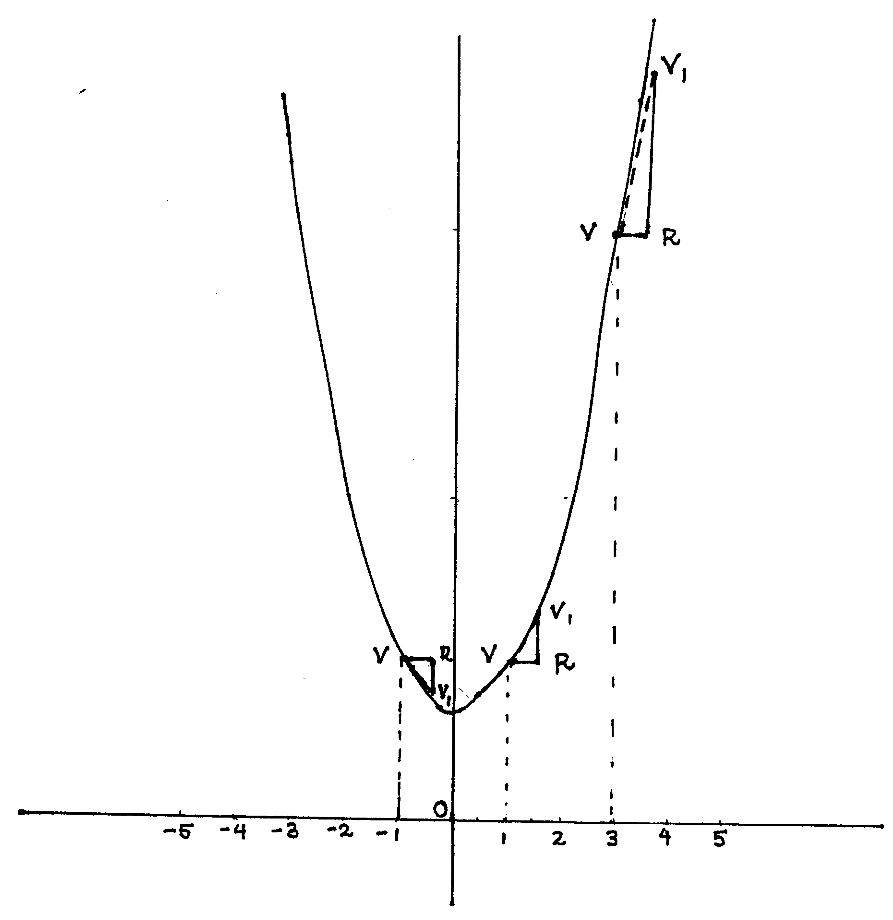
\includegraphics[width=.85\textwidth]{fig/Figure11}
\caption{}
\label{parex}
\vspace{-10pt}
\end{center}
\end{figure} 
Then
\begin{center}

$\begin{array}{ccll}
dv & = & d(x^2 + 2) & \\
 & = & d(x^2) + d(2) & \mbox{(by the addition rule)}\\
 & = & 2x\,dx + d(2) & \mbox{(by the power rule)}\\
 & = & 2x\,dx + 0 & \mbox{(by the constant rule)}\\
 & = & 2x\,dx. & 
\end{array}$
\end{center}

We can now use the equation
$$dv = 2x\,dx$$
to find the shape of the characteristic triangle for any point on the
curve.  For example, let the point $V$ be the point at which $x = 1$.
Then
$$v = x^2 + 2 = 3.$$
Let $VV_1$ be tangent to the curve at this point, and let $VV_1R$ be
the characteristic triangle.  Then $VR = dx$ and $V_1R = dv$ and
\begin{eqnarray*}
V_1R & =  & dv\\
& = & 2\,dx\\
& = & 2\,VR.
\end{eqnarray*}
The characteristic triangle $VV_1R$ at this point is therefore a right
triangle whose height is twice its base.

Again, if $V$ is the point at which $x=3$, then 
$$v= x^2 + 2 = 11,$$
and 
\begin{eqnarray*}
V_1R & = & dv\\
&= & 2(3)\,dx\\
& = & 6\,dx\\
& = & 6\,VR.
\end{eqnarray*}
The characteristic triangle $VV_1R$ at this point is therefore a right
triangle whose height is six times its base.

Finally, if $V$ is the point at which $x= -1$, then 
$$v = x^2 + 2 = 3,$$
and 
\begin{eqnarray*}
V_1R & = & dv\\
& = & -2\,dx\\
& = & -2\,VR.
\end{eqnarray*}
This means that $V_1R$ is twice as long as $VR$, but now the point
$V_1$ is {\em below} $V$, as indicated by the minus sign.

\item \label{ex2} Let $v =x^3 - 6x^2 +9x.$
Then
\begin{center}

$\begin{array}{ccll}
dv & = & d(x^3 - 6x^2 + 9x) & \\
& = & d(x^3) - d(6x^2) + d(9x) & \mbox{(addition and subtraction rule)} \\
& = & d(x^3) - 6\,d(x^2) + 9\,dx & \mbox{(constant multiple rule)} \\
& = & 3x^2\,dx - 6(2x^1\,dx) + 9\,dx & \mbox{(power rule)} \\
& = & 3x^2\,dx - 12x\,dx + 9\,dx & \mbox{(ordinary algebra)}\\
& = & (3x^2 -12x + 9)\,dx. & \mbox{(ordinary algebra)}
\end{array}$
\end{center}

Again, we could use the equation we have found for $dv$, namely
$$dv = (3x^2 -12x +9)\,dx,$$
to find the characteristic triangle for any point $V$ on the curve.
For example, if $V$ is the point at which $x= 0$, then
$$v = 0,$$
and 
\begin{eqnarray*}
V_1R & = & dv\\
& = & (0^2 - 12(0) +9)\,dx\\
& = & 9\,dx\\
& = & 9\,VR.
\end{eqnarray*}
Therefore the characteristic triangle $VV_1R$ at this point is a right
triangle whose height is nine times its base.

If $x= 2$ at $V$, then 
$$v = 2^3 - 6(2^2) + 9(2) = 2,$$
and
\begin{eqnarray*}
V_1R & = & dv\\
& = & (3(2^2) - 12(2) +9)\,dx\\
& = & -3\,dx\\
& = & -3\,VR.
\end{eqnarray*}
Therefore the characteristic triangle $VV_1R$ at this point is a right
triangle whose height is 3 times its base, and it is oriented so that
$V_1$ is below $V$.

\item Let 
$$x^2 + v^2 =1.$$ 
To find $dv$ in terms of $dx$, we take differences of both sides of
this equation.  Now $d(1) =0$, according to the constant rule.
Therefore
\begin{eqnarray*}
0 & = & d(x^2 + v^2) \\
& = & d(x^2) + d(v^2) \mbox{\hspace{5em}(addition rule)}\\
& = & 2x\,dx + 2v\,dv. \mbox{\hspace{4.4em} (power rule)}\\
\end{eqnarray*}
Therefore
$$-2x\,dx = 2v\,dv,$$
and, solving for $dv$,
$$-\frac{x}{v}\,dx = dv.$$
(If we want an expression strictly in terms of $x$, we can solve for
$v$ in terms of $x$ and substitute.  For, since
$$x^2 + v^2 = 1,$$
it follows that 
$$v^2 = 1 - x^2$$
and therefore
$$v = \sqrt{1 -x^2}.$$
Substituting into our differential equation for $dv$ then gives
$$-\frac{x}{\sqrt{1-x^2}}\,dx = dv.)$$


To interpret this differential equation geometrically, see
Figure~\ref{circex},
\begin{figure}[htp]
\begin{center}
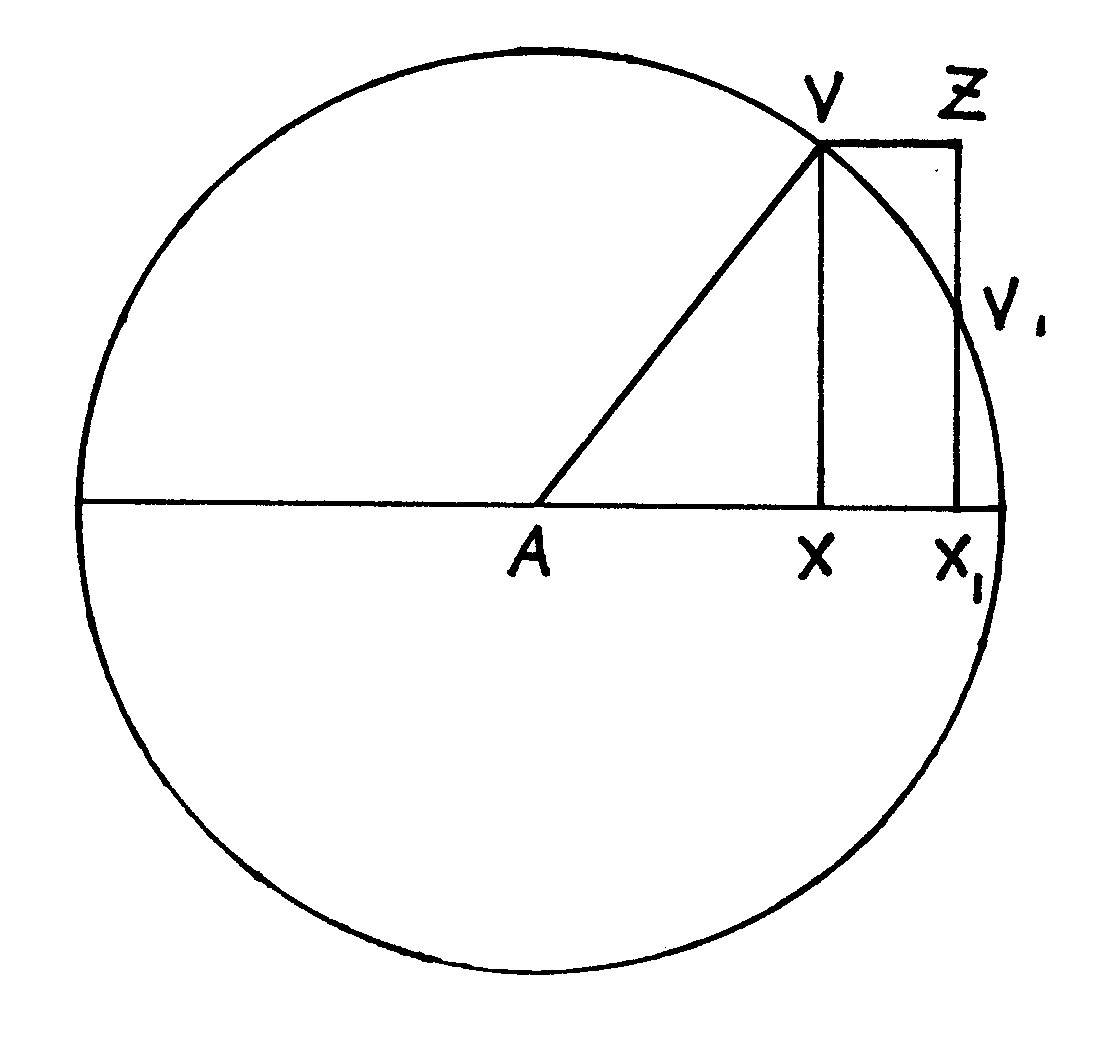
\includegraphics[width=.5\textwidth]{fig/Figure11A}
\caption{}
\label{circex}
\vspace{-10pt}
\end{center}
\end{figure}
where $AX = x$, $XV = v$, and 
$$AV = x^2 + v^2 =1.$$
The curve $VV$ is therefore a unit circle.  Let $V_1$ be infinitely
close to $V$, and draw the characteristic triangle $VZV_1,$ where
$VZ = dx$ and $dv = -ZV_1$ (where we have a minus sign because $V_1$
is below $V$).  Then our differential equation
$$-\frac{x}{v}\,dx = dv$$
becomes
$$-\frac{AX}{XV}\,VZ = - ZV_1,$$
from which it follows that
$$\frac{AX}{XV} = \frac{ZV_1}{VZ},$$
that is,
$$ AX \!:\! XV :: ZV_1 \!:\! VZ.$$
Since, in addition, angles $AXV$ and $VZV_1$ are both right, it
follows that triangle $AXV$ is similar to triangle $V_1ZV$.  Therefore
$$\angle ZVV_1 = \angle AVX,$$
and therefore
\begin{eqnarray*}
\mbox{right angle }ZVX & = & \angle ZVV_1 + \angle V_1VX\\
& = & \angle AVX + \angle V_1VX\\
& = & \angle AVV_1.
\end{eqnarray*}
Therefore the tangent $VV_1$ is perpendicular to the radius $AV$.  We
have thus used the differential calculus to give an alternate
demonstration of Proposition~III~18 in Euclid's {\em Elements}.


\item 
Let 
$$w = \frac{2x + 3}{x^2 - 5}.$$
Since $w$ is a quotient of two expressions, that is, 
$$w = \frac{v}{y},$$
where $v= 2x+3$ and $y = x^2 - 5$, we begin by using the division rule,
$$ dw = d\left(\frac{v}{y}\right) = \frac{y\,dv - v\,dy}{y^2}.$$
This is an expression for $dw$ in terms of $v$, $y$, $dv$ and $dy$,
but we want an expression in terms of $x$ and $dx$, so we have to
substitute expressions for $v$, $y$, $dv$ and $dy$ in terms of $x$ and
$dx$ into this expression for $dw$.  We already have equations for $v$
and $y$ in terms of $x$, but we have to use our rules for differences
to find expressions for $dv$ and $dy$ in terms of $x$ and $dx$.
First, let us calculate $dv$:
\begin{eqnarray*}
dv & = & d(2x + 3) \\
 & = & d(2x) + d(3) \mbox{\hspace{7.55ex} (addition rule)}\\
 & = & 2\,dx + 0 \mbox{\hspace{12ex} (constant and constant multiple rules)}\\
 & = & 2\,dx.
 \end{eqnarray*}
 
 Next, let us calculate $dy$:
 \begin{eqnarray*}
dy & = & d(x^2 - 5) \\
 & = & d(x^2) - d(5)  \mbox{\hspace{7ex} (subtraction rule)}\\
 & = & d(x^2) - 0 \mbox{\hspace{10ex} (constant rule)}\\
 & = & 2x\,dx -0 \mbox{\hspace{10ex} (power rule)}\\
 & = & 2x\,dx
 \end{eqnarray*}
 
 We now substitute our expressions for $v$, $y$, $dv$, and $dy$ into the equation given by the division rule, and simplify:
\begin{eqnarray*}
dw &  =  &  \frac{y\,dv - v\,dy}{y^2} \\
& = & \frac{(x^2-5)(2\,dx) - (2x+3)(2x\,dx)}{(x^2 - 5)^2} \mbox{\hspace{5.5ex} (substitution)}\\
& = & \frac{(2x^2 -10)\,dx - (4x^2 + 6x)\,dx}{(x^2 - 5)^2} \mbox{\hspace{8ex} (ordinary algebra)}\\
& = & \frac{(-2x^2 - 6x -10)}{x^4 -10x^2 + 25}\,dx \mbox{\hspace{18.1ex}(ordinary algebra)}
\end{eqnarray*}

The way we have calculated $dw$ in this example is typical: we started
with a complex expression for $w$ and simplified it by rewriting it in
terms of some new quantities $v$ and $y$, and then used Leibniz's
rules to find $dw$, first in terms of the new quantities and their
differences, and ultimately in terms of $x$ and $dx$. 
% This procedure
%corresponds to what is now called the {\em chain rule}.  Most modern
%presentations of the calculus need a separate rule for substitution
%because they do not treat differences as independent entities, and
%instead treat only ratios of differences; they never write $dv$ or
%$dx$ alone, but only an expression such as
%$$\frac{dv}{dx}.$$
%Modern presentations of the calculus thereby can avoid trying to
%understand $dx$ and $dv$ as infinitely small quantities, but the rules
%for differentiation become more complicated and harder to justify.  At
%any rate, if you come across a reference to the {\em chain rule} in a
%lab manual or in a textbook, you may instead use substitution,
%following the model of this and the next example.  (See also
%\cpagerefrange{chainrulestart}{chainruleend} below.)

\item \label{ex4} Let $$v = \sqrt{4x^2 - 7}.$$
Since $v$ is the square root of another expression, that is,
$$v = \sqrt[2]{y},$$
where 
$$y = 4x^2 - 7,$$
we begin by using the root rule:
$$d\sqrt[b]{y^a} = \frac{a}{b}\sqrt[b]{y^{(a-b)}}\,dy,$$
setting $a= 1$ and $b= 2$.  Substituting these values for $a$ and $b$ gives
\setlength{\jot}{2ex}
\begin{eqnarray*}
dv & = & \frac{a}{b}\sqrt[b]{y^{(a-b)}}\,dy \\
  & = & \frac{1}{2}\sqrt[2]{y^{(1-2)}}\,dy \\
      & = & \frac{1}{2}\frac{dy}{\sqrt[2]{y}}. 
\end{eqnarray*}
\setlength{\jot}{\oldjot}

This is an expression for $dv$ in terms of $y$ and $dy$, but we want
an expression in terms of $x$ and $dx$, so we have to substitute
expressions for $y$ and $dy$ in terms of $x$ and $dx$ into this
expression for $dv$.  We already have an equation for $y$ in terms of
$x$, but we have to use our rules for differences to find an
expression for $dy$ in terms of $x$ and $dx$:
\begin{eqnarray*}
dy & = & d(4x^2 -7)\\
 & = & d(4x^2) - d(7) \mbox{\hspace{7.4ex} (addition rule)}\\
 & = & 4\,d(x^2) - 0 \mbox{\hspace{10ex} (constant and constant multiple rules)}\\
 & = & 4(2x\,dx) \mbox{\hspace{12.5ex} (power rule)}\\
 & = & 8x\,dx.
 \end{eqnarray*}


We now substitute for $y$ and $dy$ in the equation for $dv$:
\setlength{\jot}{2ex}
\begin{eqnarray*}
dv & = & \frac{1}{2}\frac{dy}{\sqrt[2]{y}}  \\
& = &  \frac{1}{2}\frac{8x\,dx}{\sqrt[2]{4x^2-7}}  
 \end{eqnarray*}
\setlength{\jot}{\oldjot}



We could also calculate $dv$ by using the power rule.  If we again set $y= 4x^2 -7$, then
$$v  =  y^{\frac{1}{2}},$$
and, as we just saw,
$$dy = 8x\,dx,$$
and therefore
\setlength{\jot}{2ex}
\begin{eqnarray*}
dv & = & d(y^{\frac{1}{2}})  \\
 & = & \frac{1}{2}(y^{-\frac{1}{2}})\,dy  \mbox{\hspace{18ex} (power rule)}\\
 & = & \frac{1}{2}\frac{1}{y^{\frac{1}{2}}}\,dy \mbox{\hspace{20.6ex} (ordinary algebra)} \\
  & = & \frac{1}{2}\frac{1}{(4x^2 - 7)^{\frac{1}{2}}}8x\,dx \mbox{\hspace{9.7ex} (substitution)} \\
 & = & \frac{4x}{\sqrt{4x^2-7}}\,dx.  \mbox{\hspace{14.55ex} (ordinary algebra)}
 \end{eqnarray*}
 \setlength{\jot}{\oldjot}

\item \label{ex5} Let
$$v = (3x - 8)^{19}.$$
Then 
$$v = y^{19},$$
where 
$$y = 3x- 8.$$
According to the power rule,
$$dv = 19y^{18}\,dy.$$

To find $dy$, we use the addition rule, constant rule and constant multiple rule:
\begin{eqnarray*}
dy & = & d(3x) - d(8) \\
 & = & 3\,dx.
 \end{eqnarray*}


Substituting in for $y$ and $dy$ in the expression for $dv$, we get
\begin{eqnarray*}
dv & = & 19(3x-8)^{18}(3\,dx) \\
 & = & 57(3x - 8)^{18}\,dx.
\end{eqnarray*}

\item \label{ex6} Let 
$$v = (x+2)^5(x-7)^4.$$
Since $v$ is the product of two other expressions, we use the multiplication rule.  In fact, 
$$v = wy,$$
where 
$$w = (x+2)^5$$
and
$$y = (x-7)^4.$$
According to the multiplication rule,
$$dv = w\,dy + y\,dw.$$
This is an expression for $dv$ in terms of $w$, $y$, $dw$, and $dy$,
but we want an expression in terms of $x$ and $dx$, so we have to find
$dw$ and $dy$ in terms of $x$ and $dx$.

First, to find $dw$, we note that $w$ is a power of another quantity; namely,
$$w = z^5,$$
where 
$$z = x+2.$$
According to the power rule,
$$dw = 5z^4\,dz.$$
According to the addition and constant rules,
$$dz = dx + d(2) = dx.$$
Substituting this expression for $dz$ into our expression for $dw$, we get
$$dw = 5z^4\,dx.$$
Substituting $(x+2)$ for $z$ gives
$$dw = 5(x+2)^4\,dx.$$

Next, to find $dy$, we note that 
$$y = u^4,$$
where 
$$u = x -7,$$
so that, according to the power rule,
$$dy = 4u^3\,du.$$
According to the addition and constant rules, 
$$du = d(x) - d(7) = dx,$$
and, substituting for $u$ and $du$ in our expression for $dy$, we get
$$dy = 4(x-7)^3\,dx,$$

Putting it all together, we substitute these expressions for $dy$ and
$dw$, along with our expressions for $y$ and $w$, into our equation
for $dv$:
\begin{eqnarray*}
dv & = & w\,dy + y\,dw \\
& = & \left[(x+2)^5\right]\left[4(x-7)^3\,dx\right] + \left[(x-7)^4\right]\left[5(x+2)^4\,dx\right] .
\end{eqnarray*}
 
 
\end{enumerate}


\subsubsection*{2. Problems about finding differences}
For each of the following expressions for $v$, find $dv$ in terms of $x$ and $dx$.\label{pset1}

\begin{enumerate}
\itemsep0em
\item $$v = x^2 -3x.$$
\item $$v = x^2 + 2x - 5.$$
\item $$ v = x^3 + 4x - 6.$$
\item $$v = 2x^3 - 3x^2 - 12x + 2.$$
\item $$ x^2 + \frac{v^2}{4} = 1.$$
\item $$ x^2 - \frac{v^2}{4} = 1.$$
\item $$ v = \frac{x}{3x +2}.$$
\item  $$v = \frac{2x-1}{x+2}.$$
\item $$ v = \frac{2x^2+ 1}{x^2 - 3x}.$$
\item $$v = \frac{x^2}{3x^2 - 4}.$$
\item $$ v = \sqrt{3 - 4x}.$$
\item $$v = \sqrt{3x + 2}.$$
\item $$ v = \sqrt{x^2 + 2x -1}.$$
\item $$v = \sqrt{x^3 - x + 1}.$$
\item $$ v = (x+2)^8.$$
\item $$v = (x^2 + 4)^7.$$
\item $$ v = (x^2 -3x + 6)^5.$$
\item $$v = (x^3 - 2x)^4.$$
\item $$ v = (x+ 1)^4(3x-2)^2.$$
\item $$v = (x-3)^6(2x+1)^3.$$
\item $$ v= (x^2 + x + 1)^4(x^2 -5)^7.$$
\item $$v= (x^2 + 1)^3(3x^3 -2x)^5.$$
\item $$v = \frac{(x-1)^3(x+2)^5}{x^2 +3}.$$
\item $$v = \frac{(x +2)^2(x -3)^3}{2x +5}.$$

\end{enumerate}

\subsubsection*{3. Demonstrations of Leibniz's rules}

\subsubsection*{The constant rule}

To see why $da =0$, consider Figure~\ref{conrule}.
\begin{figure}[htp]
\begin{center}
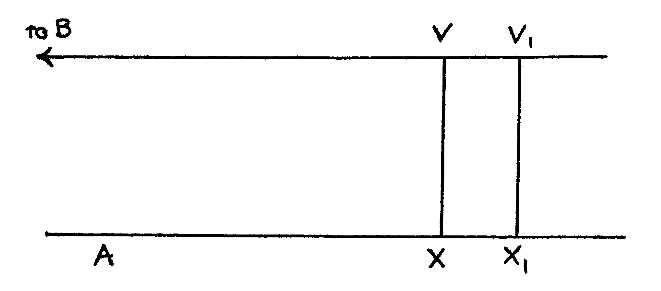
\includegraphics[width=.75\textwidth]{fig/Figure12}
\caption{}
\label{conrule}
\vspace{-10pt}
\end{center}
\end{figure}
  There we have drawn the line $VV_1$ parallel to the axis $AX$, so that $VX =V_1X_1 = a$.   If, as in Note 3,
$$ da = V_1X_1 - VX,$$
then clearly $da =0$.

Note that it is difficult to apply Leibniz's first definition of $d$
in this case.  For that definition would require that
$$da \!:\! dx :: a \!:\! XB,$$ 
where $B$ is the point where the tangent at $V$ meets the axis, but in
this case there is no such point.  Even if we treat the line $VV_1$ as
its own tangent, it does not meet the axis $AX$.  But if we were to
suppose that $VV_1$ meets the axis $AX$ at a point $B$ infinitely far
to the left of the point $A$ on the axis $AX$, then the ratio
$a \!:\! XB$ would be the ratio of a finite quantity to an infinite
one, and therefore so would the ratio $da \!:\! dx.$ In other words,
$da$ would be infinitely small compared to $dx$.  It would therefore
be reasonable to assume that $da= 0$.


What is true in this case is true more generally: it is easier to
justify Leibniz's rules by treating expressions like $dv$ as directly
representing differences between two infinitely close ordinates,
rather than trying to use the proportion Leibniz gives us:
$$dv \!:\! dx :: v \!:\! XB.$$

\subsubsection*{The constant multiple rule}

We can prove Leibniz's claim that $d(ax) = a\,dx$ as follows.  See Figure~\ref{concoeff}. 
\begin{figure}[htp]
\begin{center}
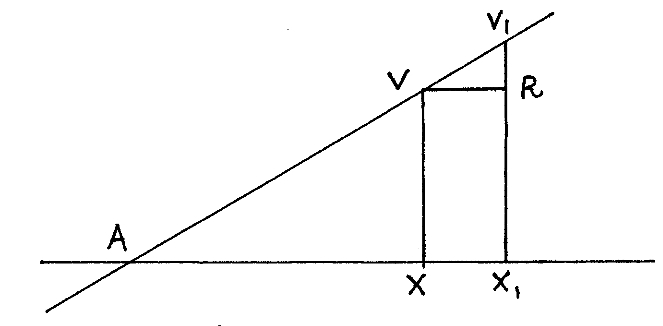
\includegraphics[width=.75\textwidth]{fig/Figure13}
\caption{}
\label{concoeff}
\vspace{-10pt}
\end{center}
\end{figure} There $AX=x$, $VX =v$, and $v =ax$. Let $V_1$ be
infinitely close to $V$, $V_1X_1 =v_1$ and $AX_1 =x_1$, and let $V_1$
be on the line $AV$ extended, so that
$$v_1=ax_1.$$
Therefore 
$$dx = x_1 -x,$$
and
$$dv = v_1 - v =  ax_1 -ax = a(x_1 - x) = a\,dx.$$
There is thus no need to use Leibniz's proportion, and in fact there
is no need to refer to the diagram at all.  We could simply have
treated $dv$ as a difference of two infinitely close values of $v$ and
followed the rules of algebra.

\subsubsection*{The addition rule}

Since 
$$z-y+w+x = v,$$
\begin{eqnarray*}
dv = v_1 - v &  =  & (z_1 - y_1 + w_1 + x_1) - (z - y + w + x) \\
 & = & (z_1 - z) - (y_1 - y) + (w_1 -w) + (x_1 -x) \\
 & = & dz - dy + dw + dx,
 \end{eqnarray*}
 just as Leibniz asserts.
 
 \subsubsection*{The multiplication rule}
 
 Leibniz gives the following argument for the multiplication rule in a
 later paper, ``A Remarkable Symbolism of the Algebraic and the
 Infinitesimal Calculus in the Comparison of Powers and Differences,
 and on the Transcendental Law of Homogeneity (published in 1710 in
 {\em The Berlin Miscellany for the Growth of the
   Sciences}).\footnote{We have changed the name of a quantity in
   this later paper to make the names correspond to those of ``A New
   Method."}
 \begin{quote}
First, 
$$d(xv) = v\,dx + x\,dv,$$
as we showed once, when many years ago we first published the
differential calculus; from this one foundation all the rest of the
calculus of differences may be demonstrated.  Now this foundation may
be shown as follows: $d(xv)$ is the difference between $(x+dx)(v+dv)$
and $xv$, or between the next rectangle and the given rectangle.  And
$$(x+dx)(v+dv) = xv + v\,dx + x\,dv + dx\,dv,$$
which, if you take away $xv$, becomes
$v\,dx + x\,dv + dx\,dv;$
but because $dx$ or $dv$ is incomparably less than $x$ or $v$, $dx\,dv$ will
also be incomparably less than $x\,dv$ and $v\,dx$, and is therefore thrown
away, and finally
$$(x+dx)(v+dv) - xv = v\,dx + x\,dv.$$
\end{quote}

 
Because $dx$ is infinitely small compared to $x$, the product $dx\,dv$
will be infinitely small compared to $x\,dv$. For
$$dx \!:\! x :: dx\,dv \!:\! x\,dv.$$
Likewise, because $dv$ is infinitely small compared to $v$, the
product $dx\,dv$ will be infinitely small compared to $v\,dx$.  The
term $dx\,dv$ is therefore infinitely small compared to the other two
terms on the right side of the equation: $x\,dv$ and $v\,dx.$ What
$dx\,dv$ adds to these two terms is therefore negligible, so that we
can leave it out of the equation and write
$$d(xv) = x\,dv + v\,dx,$$
just as Leibniz says.  The general principle here is that {\em adding}
an infinitely smaller quantity (e.\ g.\ $dw$) does not change a
quantity ($w = w+ dw$); multiplying or dividing by an infinitely
smaller quantity, however, does change a quantity ($w\,dw \neq w$).

\label{levels} This argument depends on there being two different
levels of infinitely small quantities, where a quantity on one level
($dx\,dv$) is infinitely small compared to infinitely small quantities
on another level ($x\,dv$ and $v\,dx$).  In fact there are infinitely
many different levels of infinitely small quantities, where the
quantities on one level are infinitely small compared to those on the
previous level.  For we have an infinite geometric series:
$$1,\, dx,\, (dx)^2,\, (dx)^3,\, (dx)^4,\, \mbox{etc.,}$$
where each term is infinitely small compared to the previous one.  The
difference $dx$ is an infinitely small part of the unit, $(dx)^2$ is
equal to an infinitely small part of $dx$, $(dx)^3$ is equal to an
infinitely small part of $(dx)^2$, and so on to infinity.  We could
imagine the unit divided into infinitely many infinitely small parts
equal to $dx$, $dx$ in turn divided into infinitely many infinitely
small parts equal to $(dx)^2$, and so on.  In the {\em Monadology},
Leibniz writes:
\begin{quotation}
  65. And the author of nature has been able to practice this divine
  and infinitely marvelous art, because each portion of matter is not
  only divisible to infinity, as the ancients have recognized, but is
  also actually subdivided without end, each part divided into parts
  having some motion of their own; otherwise, it would be impossible
  for each portion of matter to express the whole universe \ldots

  66. From this we see that there is a world of creatures, of living
  beings, of animals, of entelechies, of souls in the least part of
  matter.

  67. Each portion of matter can be conceived as a garden full of
  plants, and as a pond full of fish.  But each branch of a plant,
  each limb of an animal, each drop of its humors, is still another
  such garden or pond.\footnote{The translation is by Roger Ariew and
    Daniel Garber in their collection of Leibniz's {\em Philosophical
      Essays} (1989, pages 221--222).}
\end{quotation}

\subsubsection*{The division rule}


To see why the division rule is correct, we begin with the equation
Leibniz uses to define $z$, namely,
$$\frac{v}{y} = z ,$$
and multiply both sides by $y$ to get
$$v= zy.$$
We will take differences of both sides of this equation, using the
multiplication rule Leibniz has just given us, and solve for $dz$, as
follows.

First, the multiplication rule gives us
\setlength{\jot}{1.5ex}
\begin{eqnarray*}
dv & = & d(zy)\\
& = & z\,dy  + y\,dz
\end{eqnarray*}
Subtracting $z\,dy$ from both sides, we get
$$dv - z\,dy = y\,dz.$$
Substituting $\frac{v}{y}$ for $z$ on the left side of this equation gives
$$ dv - \frac{v}{y}\, dy = y\,dz.$$
Therefore, dividing both sides by $y$, we get
\setlength{\jot}{1.5ex}
\begin{eqnarray*}
dz & = & \frac{dv}{y} - \frac{v}{y^2}\,dy\\
& = & \frac{y\,dv}{y^2} - \frac{v}{y^2}\,dy\\
& = & \frac{y\,dv - v\,dy}{y^2}.
\end{eqnarray*}
\setlength{\jot}{\oldjot}
This last expression is the formula for $dz$ in the division rule.

\subsubsection*{The power rule}

This rule,
$$d(x^a) = ax^{(a-1)}\,dx,$$
is in fact a series of rules, one for every positive whole number $a$.
To see why it is correct, we go through the cases in order.

To begin, if $a=1$, then
$$d(x^a) = dx,$$
while 
$$ax^{(a-1)}\,dx = 1x^{(1-1)}\,dx = dx,$$
and therefore
$$d(x^a) = ax^{(a-1)}\,dx,$$
as the rule requires.


If $a=2$, then $x^2$ is $x$ multiplied by $x$, and so we can apply the
multiplication rule that Leibniz has given us:
\begin{eqnarray*}
d(x^2)&  = & d(x\cdot x) \\
 & = & x\,dx + x\,dx \mbox{ (by the multiplication rule)}\\
  & = & 2x\,dx \\
  & = & 2x^{(2-1)}\,dx,
 \end{eqnarray*}
as the rule requires.

If $a=3$, then $x^3$ is $x$ multiplied by $x^2$, and so we can apply
the multiplication rule:
\begin{eqnarray*}
d(x^3) & = & d(x\cdot x^2) \\
 & = & x\,d(x^2) + x^2\,dx.
 \end{eqnarray*}
 We just saw that $d(x^2)$ is equal to $2x\,dx$, so we substitute the
 latter for the former, and therefore
\begin{eqnarray*}
d(x^3) & = & x(2x\,dx) + x^2\,dx \\
 & = & 2x^2\,dx + x^2\,dx \\
  & = & 3x^2\,dx \\
   & = & 3x^{(3-1)}\,dx,
 \end{eqnarray*}
as the rule requires.

Likewise, 
\begin{eqnarray*}
d(x^4) & = & 4x^3\,dx,\\
d(x^5) & = & 5x^4\,dx,
\end{eqnarray*}
and so on.

We could continue in this way indefinitely.  The rule for each power
would follow from the rule for the previous power once we use the
multiplication rule: if we have shown the rule is correct for some
power $a$, so that
$$d(x^a) = ax^{(a-1)}\,dx,$$
then we can show the rule is correct for $a+1$ by first noting that 
$$x^{(a+1)} = x \cdot x^a,$$ 
and using the multiplication rule,
$$d(x^{(a+1)}) = x\,d(x^a) + x^a\,dx,$$
and then substituting $ax^{(a-1)}\,dx$ for $dx^a$ (we assumed we have
already shown that the rule is true for $x^a$), so that we get
\begin{eqnarray*}
d(x^{(a+1)}) & = & x(ax^{(a-1)}dx) + x^a\,dx \\
& = & ax^a\,dx + x^a\,dx \\
& = & (a+1)x^a\,dx,
\end{eqnarray*}
as the rule requires.  Beginning from the rule for $a$ we would thus
have shown the rule for $a+1$.  In this way we would eventually show
the rule is correct for any possible (positive whole number) power.

\subsubsection*{The power rule for negative exponents}

To see why 
$$d\left(\frac{1}{x^a}\right) = - \frac{a\,dx}{x^{(a+1)}},$$
we begin by using the division rule:
$$d\left(\frac{1}{x^a}\right) = \frac{x^a\,d(1) - 1\,d(x^a)}{(x^a)^2}.$$
To simplify the expression on the right, we note that $d(1) = 0$ (by
the constant rule), and use the power rule to substitute
$ax^{(a-1)}\,dx$ for $d(x^a)$.  We get \setlength{\jot}{1.5ex}
\begin{eqnarray*}
d\left(\frac{1}{x^a}\right) & = & \frac{x^a\,d(1) - 1\,d(x^a)}{(x^a)^2}\\
& = & \frac{0 -ax^{(a-1)}\,dx}{(x^a)^2} \\
& = & \frac{-ax^{(a-1)}\,dx}{x^{2a}}\\
& = & \frac{-a\,dx}{x^{(2a-(a-1))}}\\
& = & -\frac{a\,dx}{x^{(a+1)}}
\end{eqnarray*}
\setlength{\jot}{\oldjot}
This last expression is the one Leibniz gives in his rule.



\subsubsection*{Root rule}

To see why 
$$d(\sqrt[b]{x^a}) = \frac{a}{b}\,dx\,\sqrt[b]{x^{(a-b)}},$$
 we begin by setting
$$y = \sqrt[b]{x^a}.$$
Then
\begin{eqnarray*}
y^b & = & x^a, \mbox{ and}\\
d(y^b) & = & d(x^a)
\end{eqnarray*}
Applying the power rule to both sides of this equation gives
$$by^{(b-1)}\,dy = ax^{(a-1)}\,dx.$$
Solving for $dy$, we get
$$dy = \frac{ax^{(a-1)}\,dx}{by^{(b-1)}}.$$
Since we want an expression for $dy$ purely in terms of $x$, we
substitute $\sqrt[b]{x^a}$ for $y$ in this expression, and simplify.
There are many steps, but we only need ordinary algebra, including
especially the rules for exponents: \setlength{\jot}{2ex}
\begin{eqnarray*}
dy & = & \frac{ax^{(a-1)}\,dx}{b(\sqrt[b]x^a)^{(b-1)}}\\
 & = & \frac{ax^{(a-1)}}{b(x^{(\frac{a}{b})})^{(b-1)}}\,dx\\
 & = & \frac{ax^{(a-1)}}{b(x^{(\frac{a}{b}(b-1))})}\,dx\\
 & = & \frac{ax^{(a-1)}}{b(x^{(a- \frac{a}{b})})}\,dx\\
 & = & \frac{a}{b} x^{((a-1) - (a- \frac{a}{b}))}\,dx\\
 & = & \frac{a}{b} x^{(\frac{a}{b} - 1)}\,dx\\
 & = & \frac{a}{b} x^{(\frac{1}{b}(a- b))}\,dx\\
 & = & \frac{a}{b} (x^{(a-b)})^\frac{1}{b}\,dx\\
 & = & \frac{a}{b} \sqrt[b]{x^{(a-b)}}\,dx
\end{eqnarray*}
\setlength{\jot}{\oldjot}
This last expression is the one Leibniz gives in his rule.

A similar argument may be used to show that Leibniz's rule for 
$$d\left(\frac{1}{\sqrt[b]{x^a}}\right)$$
is correct.


\subsubsection*{4. Examples of finding greatest and least ordinates}
\begin{enumerate}
\item Let $v = x^2 + 2.$ We want to find the points where $v$ is
  greatest or least.  As Leibniz observed earlier
  (page~\pageref{dvzero}), at a point where $v$ is a greatest or least
  ordinate, $dv=0$; there the differences of $v$ are neither positive
  nor negative, and $v$ is neither increasing nor decreasing.
  Therefore we have to find points where $dv =0$.  In the first
  example of finding differences (page~\pageref{ex1}, above) we
  calculated $dv$, showing that
$$dv = 2x\,dx.$$
We have assumed that $dx$ is always positive, and therefore $dv$ is
greater than 0 when $x$ is positive, less than 0 when $x$ is negative,
and equal to 0 precisely when $x =0$.  Therefore when $x$ is positive
and increasing, $v$ is also increasing; when $x$ is negative and
increasing (that is, when $x$ is negative but is becoming less
negative), then $v$ is decreasing; and when $x$ is 0, $v$ is at its
least.  When $x$ is 0, $v = x^2 + 2 =2$, and therefore the least
ordinate $v$ is equal to 2. See Figure~\ref{glex1}.
\begin{figure}[htp]
\begin{center}
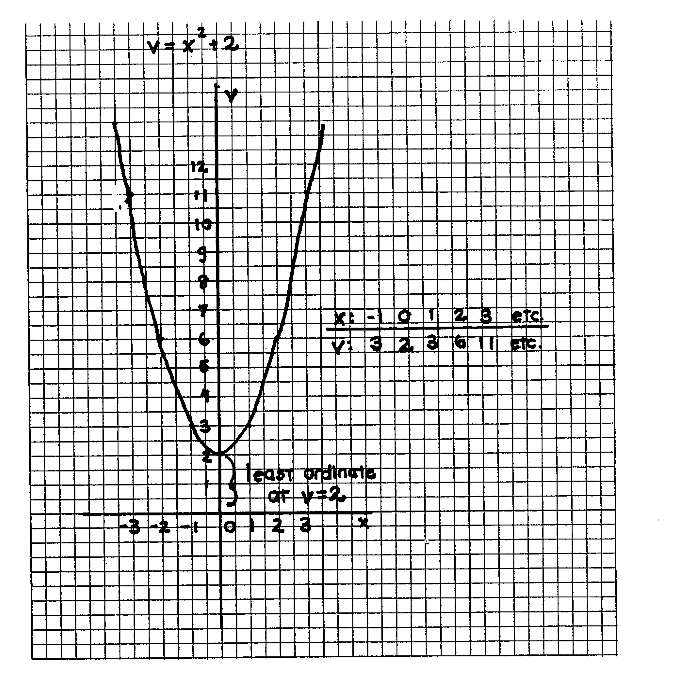
\includegraphics[width=\textwidth]{fig/Figure14}
\caption{}
\label{glex1}
\vspace{-10pt}
\end{center}
\end{figure}

\item \label{minex3} Let $v = x^3 - 6x^2 + 9x.$ We want to find the points where $v$
  is greatest or least, and we again begin by finding where $dv$ is
  positive, where it is negative, and where it is 0.  As we saw in the
  second example (page~\pageref{ex2}, above),
$$dv = (3x^2 - 12x + 9)\,dx.$$
To find out where $dv$ is positive, negative, or zero, we factor the
expression on the right:
$$dv = 3(x-1)(x-3)\,dx.$$
When $x=1$, then $x-1 = 0$, and therefore $dv = 0$.  When $x=3$, then
$x-3 =0$ and $dv=0$.  When $x<1$, then $dv$ is the product of two
negative quantities (namely, $(x-1)$ and $(x-3)$) and two positive
quantities (3 and $dx$), and is therefore positive.  When $1<x<3$,
then $dv$ is the product of one negative quantity ($(x-3)$) and three
positive quantities (3, $(x-1)$, and $dx$), and is therefore negative.
Finally, when $x>3$, $dv$ is the product of four positive quantities,
and is therefore positive.  It follows from all this that $v$ is
increasing when $x<1$, at a greatest value when $x=1$, decreasing when
$1<x<3$, at a least value when $x=3$, and increasing again when $x>3$.
When $x=1$,
$$v = 1^3 - 6(1^2) + 9(1) = 4,$$
so that 4 is a greatest value for the ordinate $v$.  When $x=3$, 
\begin{eqnarray*}
v & = & 3^3 - 6(3^2) +9(3) \\
 & = & 27 - 54 +27  \\
 & = & 0,
 \end{eqnarray*}
 so that 0 is a least value for the ordinate $v$.  See Figure~\ref{glex2}.
 \begin{figure}[htp]
\begin{center}
  % \includegraphics[width=.85\textwidth]{fig/Figure15}
    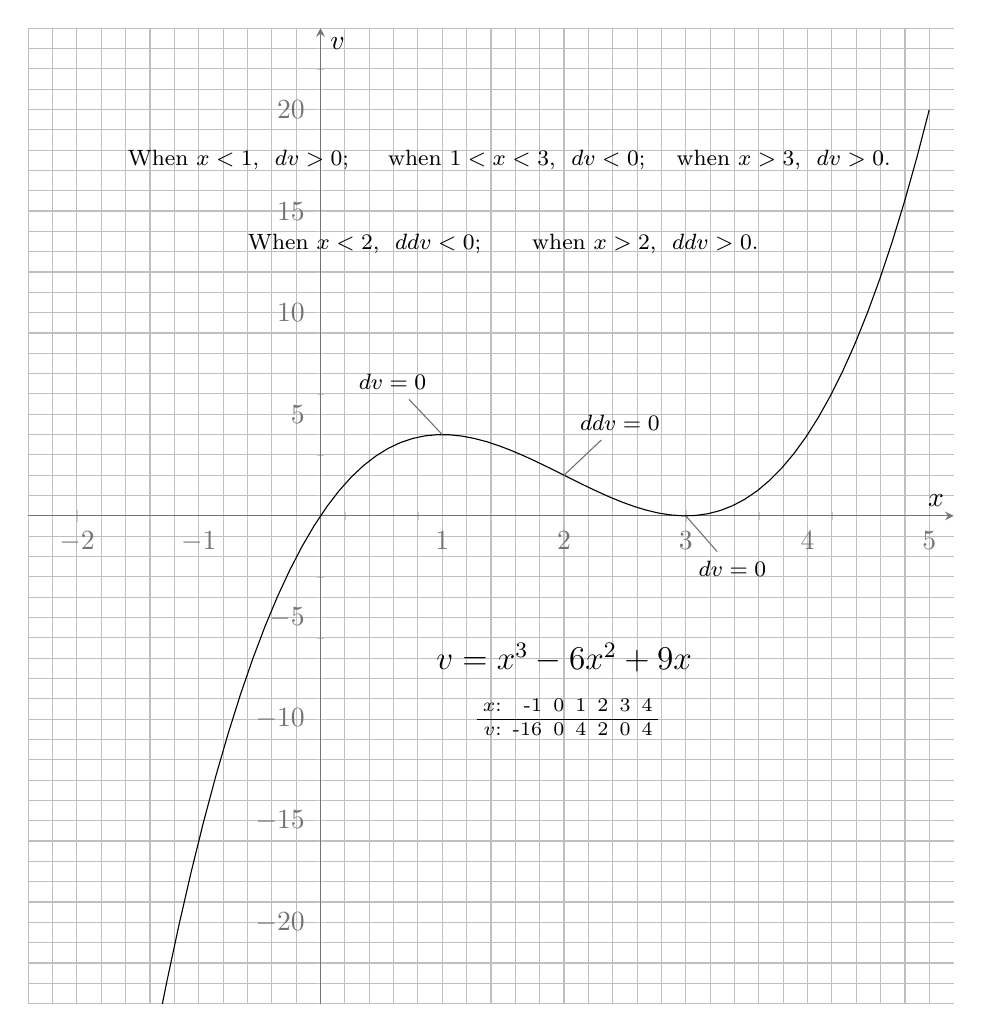
\begin{tikzpicture}
    \tikzset{every pin edge/.style={black!55}} 
    \begin{axis}[axis line style={black!55},
      axis lines=middle,
      %label style={black},%!45},
      xlabel={$x$}, ylabel=$v$,
      % grid style={black!20},
      xmajorgrids=true, ymajorgrids=true,
      xminorgrids=true, yminorgrids=true,
      tick label style={black!55},
      tick style={gray!40},
      minor x tick num=4, minor y tick num=4,
      ymin=-24, ymax=24,
      xmin=-2.4, xmax=5.2,
      width=5.25in, height=5.5in,
      samples=100, ]
      \node[] at (1.55,17.5)
      {\footnotesize When $x<1,\hspace{0.5em} dv>0;$ \hspace{1em}
        when $1<x<3, \hspace{0.5em} dv<0;$\hspace{1em}
        when $x>3,\hspace{0.5em} dv>0.$};
      \node[] at (1.5,13.4) {\footnotesize When $x<2,
        \hspace{0.5em} ddv<0;$ \hspace{1.5em}
        when $x>2, \hspace{0.5em} ddv>0.$};
      \addplot [ black,] {x^3 - 6*x^2 + 9*x};
      \node[coordinate, pin=100:{\footnotesize$dv=0$}] at (1,4) {};
      \node[coordinate, pin=275:{\footnotesize$dv=0$}] at (3,0) {};
      \node[coordinate, pin=80:{\footnotesize$ddv=0$}] at (2,2) {};
      \node[] at (2,-7) {\large $v=x^3 -6x^2+ 9x$};
      \node[] at (2,-10) {\scriptsize
        \setlength{\tabcolsep}{2pt}
        \begin{tabular}{rrrrrrr}
          $x$:&-1&0&1&2&3&4\\ \hline
          $v$:&-16&0&4&2&0&4
        \end{tabular}};
    \end{axis}
  \end{tikzpicture}
\caption{}
\label{glex2}
\vspace{-10pt}
\end{center}
\end{figure} Note that $4$ is not absolutely the greatest value of
$v$, but only a value greater than all nearby values, and likewise $0$
is not absolutely the least value of $v$, but only a value less than
all the nearby values.

As Leibniz observes, by looking at where the differences of the
differences, $ddv$, are positive, negative, and 0, we can also find
where the curve whose ordinates are $v$ turns its concavity upward or
downward, and where it is inflected.  First, we need to find $ddv$;
$$ddv = d(dv)  =  d((3x^2 - 12x +9)\,dx).$$
Now we may assume that $dx$ is a constant, that is, that it is the
same infinitely small quantity at every point, no matter what $x$
is.\label{dx_constant} Then, by the constant multiple rule,
\begin{eqnarray*}
ddv & = & d(3x^2 -12x +9)\,dx \\
& = & (d(3x^2) - d(12x) + d(9))\,dx \mbox{\hspace{5.55ex} (addition rule)} \\
& = & (3d(x^2) - 12\,dx + 0)\,dx \mbox{\hspace{10ex} (constant rules)}\\
 & = & (3(2x\,dx) - 12\,dx)\,dx \mbox{\hspace{12.15ex} (power rule)}\\
 & = & (6x -12)\,(dx)^2 \mbox{\hspace{18.1ex} (ordinary algebra)}\\
 & = & 6(x-2)\,(dx)^2 \mbox{\hspace{19.25ex} (factoring)}
 \end{eqnarray*}
 Therefore,
 $$\begin{array}{cl}
 ddv < 0 & \mbox{when } x<2 \\
 ddv =0 & \mbox{when } x =2 \mbox{, and} \\
 ddv > 0 & \mbox{when } x >2.
   \end{array}$$
   Therefore the concavity of the curve is turned downward when $x<2$,
   there is an inflection point when $x=2$, and the concavity of the
   curve is turned upward when $x>2$.  See Figure~\ref{glex2}. 
 


\end{enumerate}

\subsubsection*{5. Problems about finding greatest and least ordinates}
\label{pset2} For each of the curves given by the following equations,
find the greatest ordinates, the least ordinates, where the ordinates
are decreasing and where they are increasing.  Also find where each
curve turns its concavity upward, where it turns its concavity
downward, and where it is inflected (if anywhere).  Sketch a graph of
each curve.
\begin{enumerate}
\itemsep0em
\item $v = x^2 -4x +1.$
\item  $v = x^2  + 2x - 5.$
\item $v = x^3 -3x^2 -9x +4.$
\item $v = 2x^3 - 3x^2 - 12x + 2.$
\end{enumerate}

\subsubsection*{6. Examples of finding tangents}
Recall that Leibniz initially defines $dv$ using a proportion
depending on the tangents to the curve.  In terms of
Figure~\ref{tang},
\begin{figure}[htp]
\begin{center}
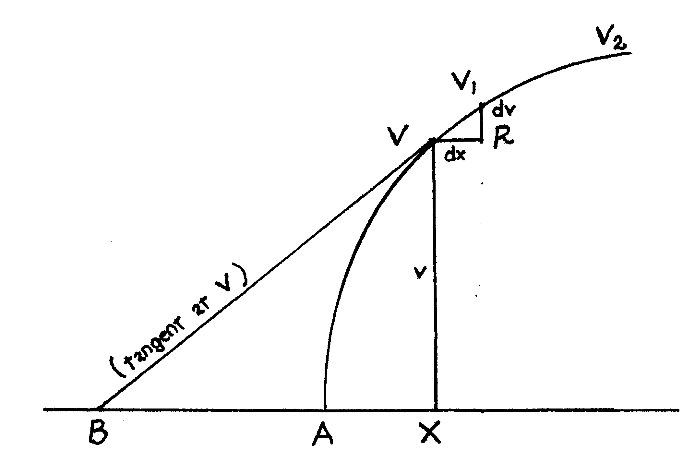
\includegraphics[width=.85\textwidth]{fig/Figure16}
\caption{}
\label{tang}
\vspace{-10pt}
\end{center}
\end{figure}
the proportion is:
$$dv \!:\! dx :: VX \!:\! XB.$$
Now if $dv=0$, then $VX$ is a greatest or least ordinate and the tangent $VB$ becomes parallel to the axis $AX$, as in Figure~\ref{htang}.
\begin{figure}[htp]
\begin{center}
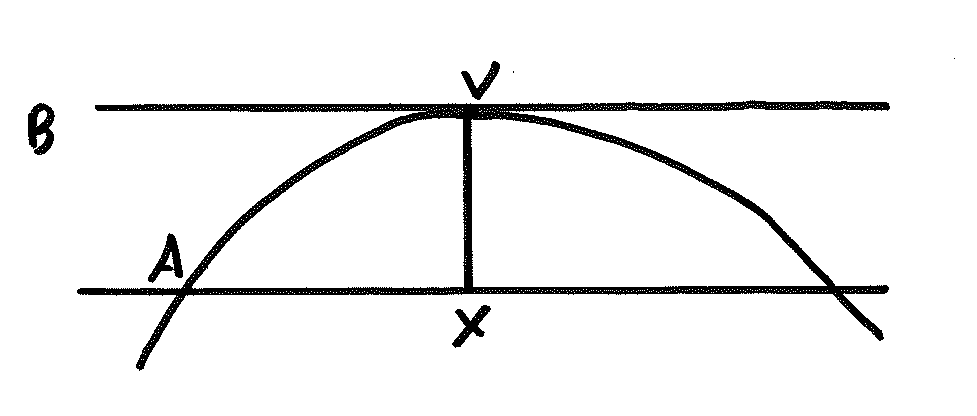
\includegraphics[width=.75\textwidth]{fig/Figure16A}
\caption{}
\label{htang}
\vspace{-10pt}
\end{center}
\end{figure}


But if $dv$ is not equal to zero, we convert the proportion
$$dv \!:\! dx :: VX \!:\! XB \mbox{ (Figure~\ref{tang})}$$
 to an equation, and solve for $XB$:
\setlength{\jot}{1.5ex}
\begin{eqnarray*}
\frac{dv}{dx} & = & \frac{v}{XB} \\
dv \cdot XB & = & v\,dx\\
XB &= &\frac{v\,dx}{dv}.
\end{eqnarray*}
Therefore, once we have $dv$ in terms of $x$ and $dx$, we can find
$XB$.  But once we have found $XB$, we can draw the tangent by
connecting $B$ and $V$.  Leibniz's calculus thus gives us a method for
finding tangents to a curve.  This method is similar to the method
Apollonius uses in Propositions~I~33 and I~34 of the {\em Conics}, in
that Apollonius also finds tangents by finding where they meet a
diameter. 

 Here are two simple examples, based on the differences we have already calculated.
\begin{enumerate}
\item Let $v = x^2 + 2.$  Then, as we saw in the first example (page~\pageref{ex1}, above),
$$dv = 2x\,dx.$$

Now $dv=0$ when $x=0$, and therefore there is horizontal tangent to the curve when $x=0$.

When $x\neq 0$, then $dv \neq 0$, and we can use the above equation for $XB$.  Therefore
\begin{eqnarray*}
XB & = & \frac{v\, dx}{dv}\\
& = & \frac{(x^2 + 2)\,dx}{2x\,dx}\\
& = & \frac{x^2 + 2}{2x}.
\end{eqnarray*}
We may use this equation to find tangents to the curve.  If for example, if $x=1$, then
$$XB = \frac{1^2 +2}{2(1)} = \frac{3}{2},$$
while if $x=-1$, then
$$XB = \frac{(-1)^2 + 2}{2(-1)} = -\frac{3}{2}.$$
The minus sign means that the point $B$ is to the right of $X$ in this
case.  See Figure~\ref{tangex1}.
\begin{figure}[htp]
\begin{center}
%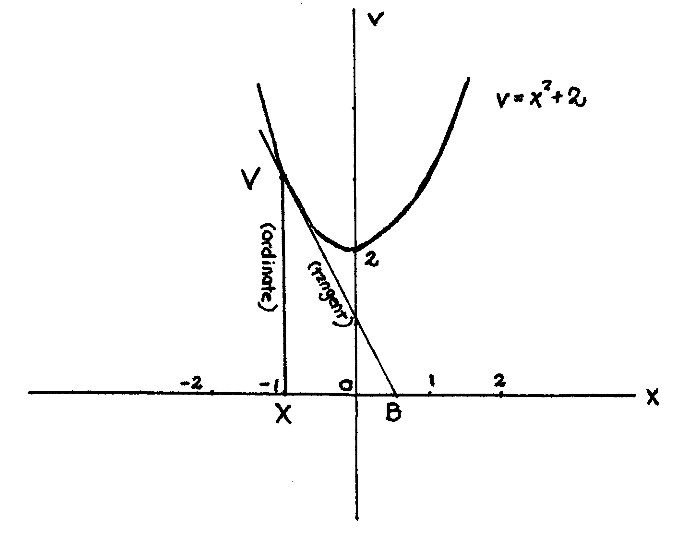
\includegraphics[width=\textwidth]{fig/Figure17}
\scalebox{0.9}{
\begin{tikzpicture}
    \begin{axis}[axis line style={black!55},
%    title={$v=x^3-6x^2+9x$},
      xlabel=$x$,
      ylabel=$v$,
      axis lines=middle,
      ymin=-1,
      ymax=4,
      xmin=-2.5,
      xmax=2.5,
      xtick distance=1, ytick distance=1,
      width=5in, height=5in, samples=100, ]
      \addplot[] {x^2 + 2};
      \node [] at (2,3.5)  {$v=x^2 + 2$};
      \addplot[] coordinates {(-1,3) (-1,0)}
      [every node/.style={xshift=-18pt,yshift=-8pt}, sloped,]
       node [pos=0.6] {\rotatebox{0}{\small (ordinate)}};
       \node at (-1.25,3) {\textsf{V}};
       \node at (-0.8,0.13) {\textsf{X}};
       \node at (0.65,0.15) {\textsf{B}};
       \addplot[] coordinates {(-1,3) (0.5,0)}
       [every node/.style={xshift=-7pt,yshift=-8pt},sloped]
       node [pos=.5] {\small (tangent)};
       \addplot[line width=0.8pt] coordinates {(-1,3) (0.5,0)};
    \end{axis}
  \end{tikzpicture}
  }
\caption{}
\label{tangex1}
\vspace{-10pt}
\end{center}
\end{figure}

\item Let $v = x^3 - 6x^2 + 9x.$ Then, as we saw in the second example (page~\pageref{ex2}, above),
$$dv = (3x^2 - 12x + 9)\,dx.$$
As we saw in the second example on page~\pageref{minex3}, $dv=0$ only when $x=1$ or $x=3$.  Therefore at these points the curve has a horizontal tangent.


But when $x \neq 1$ and $x \neq 3$, then $dv \neq 0$, and we can substitute into the above equation for $XB$, getting
\begin{eqnarray*}
XB & = & \frac{v\, dx}{dv}\\
& = & \frac{(x^3 - 6x^2 +9x)\,dx}{(3x^2 -12x +9)\,dx}\\
& = & \frac{x^3 - 6x^2 + 9x}{3x^2 - 12x + 9}.
\end{eqnarray*}
We may use this equation to find tangents to the curve.  If, for example, $x=4$, then
\begin{eqnarray*}
XB & = & \frac{(4)^3 - 6(4)^2 + 9(4)}{3(4)^2 - 12(4) + 9} \\
& = & \frac{64 - 96 + 36}{48 - 48 + 9}\\ 
& = & \frac{4}{9}.
\end{eqnarray*}
See Figure~\ref{tangex2}.
\begin{figure}[htp]
\begin{center}
  % \includegraphics[width=\textwidth]{fig/Figure18}
    \begin{tikzpicture}
    \begin{axis}[
%    title={$v=x^3-6x^2+9x$},
      xlabel=$x$,
      ylabel=$v$,
     axis lines=middle,
      ymin=-20,
      ymax=20,
      xmin=-2,
      xmax=5,
      width=5in, height=5in, samples=100, ]
      \addplot[] {x^3 - 6*x^2 + 9*x};
      \node [] at (1.5,12)  {$v=x^3 - 6x^2 + 9x$};
      \addplot[] coordinates {(4,4) (4,0)}
      [every node/.style={yshift=3pt}, sloped,]
      node [pos=.5] {\rotatebox{180}{\tiny ordinate}};
      \addplot[] coordinates {(4,4) (3.55555,0)}
      [every node/.style={yshift=-2.5pt},sloped]
      node [pos=.5] {\tiny tangent};% $9x-32$ is the tangent at (4,4)
      \addplot[line width=0.8pt] coordinates {(3.55555,0) (4,0)};
    \end{axis}
  \end{tikzpicture}
\caption{}
\label{tangex2}
\vspace{-10pt}
\end{center}
\end{figure}

\end{enumerate}
\setlength{\jot}{\oldjot}

\subsubsection*{7. Problems about finding tangents}
\label{pset3} For curves given by each of the following equations,
find a general expression for the line $XB$ cut off on the axis by the
ordinate and the tangent, and use this general expression to find one
particular tangent.
\begin{enumerate}
\itemsep0em
\item $v = x^2 -4x +1.$
\item  $v = x^2  + 2x - 5.$
\item $v = x^3 -3x^2 -9x +4.$
\item $v = 2x^3 - 3x^2 - 12x + 2.$
\end{enumerate}


\subsection*{Note 8}\label{diffeq}
\label{cnm8}

Here is an example to show what Leibniz is saying here.  Suppose the
given equation is
$$2x^2 + 3xy = 1,$$
and we want to find its differential equation.  Then the {\em terms}
of this equation are $2x^2$, $3xy$, and $1$. To write down the
differential equation for this equation, we substitute for each of
these terms its differential quantity; namely, we substitute $d(2x^2)$
for $2x^2$, $d(3xy)$ for $3xy$, and $d(1)$ for $1$.  This gives us a
differential equation:
$$d(2x^2) + d(3xy) = d(1).$$

Next, for quantities ($2$, $x$, $3$, $y$ and $1$) which are not
themselves terms, but contribute to forming terms ($2$ and $x$, for
example, contribute to forming the term $2x^2$), we do not directly
use their differential quantities.  In other words, we do {\em not}
simply substitute $dx$ for $x$, and do {\em not} substitute
$d(2)d(x)^2$ for $d(2x^2)$.  Instead, we use Leibniz's algorithm, that
is, his six rules for finding differences.  In this case, we use the
power rule, the multiplication rule, and the constant rules to get
\begin{eqnarray*}
d(2x^2) & = & 4x\,dx,\\
d(3xy) & = & 3x\,dy + 3y\,dx \mbox{ and}\\
d(1) & = & 0.
\end{eqnarray*}
We use these equations to substitute into the above differential
equation, and get our final differential equation:
$$4x\,dx + 3x\,dy + 3y\,dx = 0.$$

If our original, algebraic, equation
$$2x^2 + 3xy = 1,$$
is the equation of a curve, then the differential equation
$$4x\,dx + 3x\,dy + 3y\,dx = 0$$
is another equation for the same curve, now expressing not the
universal relation between two ordinary quanitities, $x$ and $y$, but
the universal relation between these quantities and their differences
$dx$ and $dy$.  Just as we can use the algebraic equation to solve
geometric problems, we may use the differential equation to solve for
the differences $dx$ and $dy$ and thereby find tangents or greatest
and least lines.

\subsection*{Note 9}
\label{cnm9}

A simple example of a transcendent line is the line whose equation is
$y = x^x$.  It is of no definite degree because there is a variable in
an exponent: $x$ could be $2$, $3$, $4$, or any other number, and so
we cannot say what the degree of the term $x^x$ is.  The algebraic
calculus cannot be applied to equations like this because it only
includes the five basic operations Descartes mentions at the beginning
of the {\em Geometry}: addition, subtraction, multiplication,
division, and extracting of roots.  The algebraic calculus does not
include taking exponents with variable powers, such as $x^x$.
Descartes calls all lines that can be represented by the algebraic
calculus {\em geometric}, and all other lines {\em mechanical}. (See
page 16 of the St.\ John's (1998) edition of the Geometry or page 48
of the Dover (1954) edition.) The lines Leibniz calls {\em
  transcendent} would therefore be called {\em mechanical} by
Descartes.

\subsection*{Note 10}
\label{cnm10}

We will come back to Leibniz's discussion of how the calculus extends
to transcendent lines in the following paper, ``On Recondite
Geometry."  We define the cycloid and find its transcendent equation
in the notes to ``On Recondite Geometry"
(pages~\pageref{cycloid}--\pageref{ecycloid}, below).

\subsection*{Note 11}
\label{cnm11}

The law of homogeneity for differential quantities requires that all
terms in an equation be of the same level of infinity (see the remarks
after the demonstration of the multiplication rule on
page~\pageref{levels}, above).  If one term of an equation is at the
first level of infinitely small quantities, the level of simple
differences such as $dx$, then all terms must be at that level.  If
one term of an equation is at the second level of infinitely small
quantities, such as $(dx)^2$, then all terms must be at that level,
and so on.  This law thus guarantees that no term will be infinitely
small or infinitely large compared to any other term in the equation.

The law of homogeneity for differential quantities would, in general,
require that in each term of an equation, the sum of the exponents of
the differences is always the same.  For example, in the term
$$(dx)^2dy\,dz$$
the sum of exponents is 4: $dx$ has exponent 2, while $dy$ and $dz$
each have exponent 1 ($dy = dy^1$ and $dz = dz^1$).  Such a term would
be at the fourth level of infinitely small quantities.  It could
therefore be combined with any other terms for which the sum of
exponents is 4 to make a homogeneous differential equation.  For
example, we could combine it with $(dy)^2(dz)^2$ and $(dx)^4$ to make
the homogeneous differential equation
$$(dx)^2dy\,dz  + (dy)^2(dz)^2 = (dx)^4.$$

Note that only the differential quantities matter for Leibniz's law of
homogeneity; any other finite quantities that go to make up a term do
not affect the level of infinity of the term.  For example, in the
term
$$2x^2(dx)^2dy\,dz$$
the sum of the exponents of {\em differences} is still 4 (the exponent
of $dx$ is 2, and the exponents of $dy$ and $dz$ are 1), and this term
is therefore on the fourth level of infinitely small quantities.  The
exponent of the finite quantity $x$ does not affect the level of the
term.  This term could be combined with other terms on the fourth
level of infinitely small quantities to make a homogeneous
differential equation, such as
$$2x^2(dx)^2dy\,dz + z(dy)^2(dz)^2 = (x + 2yz)(dx)^4.$$

In the case Leibniz is discussing in the text, in each term of the
differential equation the sum of the exponents of the differences is
always 1: each term has either $dx^1$ or $dy^1$, and no other
differences.

Leibniz's law of homogeneity is analogous to Vi\`{e}te's algebraic law
of homogeneity (see Chapter III of his {\em Introduction to the
  Analytic Art}), which requires that each term of an equation
represent a magnitude of the same dimension, or what amounts to the
same thing, that in each term the sum of the exponents of all the
quantities in that term be the same.

\subsection*{Note 12}
\label{cnm12}

Leibniz is thinking of something moving from the point $C$ to the
point $F$ along line $CF$ (see Figure~\ref{leasttimeA}),
\begin{figure}[htp]
\begin{center}
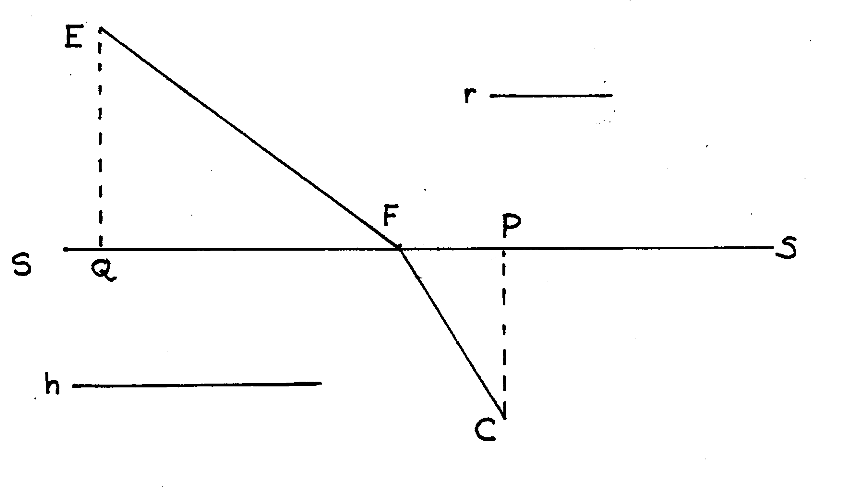
\includegraphics[width=.85\textwidth]{fig/Figure21}
\caption{}
\label{leasttimeA}
\vspace{-10pt}
\end{center}
\end{figure} and then from $F$ to $E$ along line $FE$.  By {\em
  density} he means the power of the medium to resist motion, so that
the total difficulty of any motion in a uniform medium is equal to the
product of the density of that medium and the length of the path along
which the motion occurs.  (Leibniz apparently is treating densities as
lines, so that the product of a density and a line is a rectangle.)
Therefore, $CF$ times $h$ is equal to the difficulty of the motion
from $C$ to $F$, $EF$ times $r$ is equal to the difficulty of the
motion from $F$ to $E$, and
$$(CF)\cdot h + (EF) \cdot r$$
is equal to the total difficulty of the motion from $C$ to $E$.  Now
this difficulty is variable because the point $F$ is variable: $F$
could be anywhere on the line $SS$.  Leibniz wants to find where $F$
has to be for the motion to be as easy as possible, that is, he wants
to find the point $F$ so that
$$(CF)\cdot h + (EF) \cdot r$$
is as small as possible.

As Leibniz suggests later, this example may be applied to optics.
Suppose light moves from the point $C$ to the point $F$ along the line
$CF$, and from the point $F$ to the point $E$ along the line $FE$.  We
take the density of a medium to be inversely proportional to the speed
with which light moves in that medium, so that if the light moves with
speed $v_w$ in the water below $SS$, and with speed $v_a$ in the air
above $SS$, then the density $h$ of the water is equal to
$$\frac{1}{v_w},$$
while the density $r$ of the air is equal to 
$$\frac{1}{v_a}.$$
If we call the time the light takes to move along $CF$ in the water
$t_w$, and the time it takes the light to move along $FE$ in the air
$t_a$, then
\begin{eqnarray*}
v_w & = & \frac{CF}{t_w}, \mbox{ and}\\
v_a & = & \frac{FE}{t_a}.
\end{eqnarray*}
Therefore the difficulty of the motion along $CF$, 
\setlength{\jot}{2ex}
\begin{eqnarray*}
(CF)\cdot h &  =  & (CF) \cdot \frac{1}{v_w}\\
& = & (CF) \cdot \frac{1}{\left(\frac{CF}{t_w}\right)}\\
& = & (CF) \cdot \frac{t_w}{CF} \\
& = & t_w;
\end{eqnarray*}
that is, the difficulty of the motion is in this case equal to the
time.  Likewise, the difficulty of the motion from $F$ to $E$ along
the line $FE$ is equal to the time $t_a$, and therefore the difficulty
of the whole motion from $C$ to $E$ is equal to the time it takes.  In
this case Leibniz is therefore looking for the path light could take
that will take the least time to get from $C$ to $E$.
\setlength{\jot}{\oldjot}

\subsection*{Note 13}
\label{cnm13}

Leibniz is defining the curve $VV$ so that when $GK$ (in Figure~\ref{leasttime2A})
\begin{figure}[htp]
\begin{center}
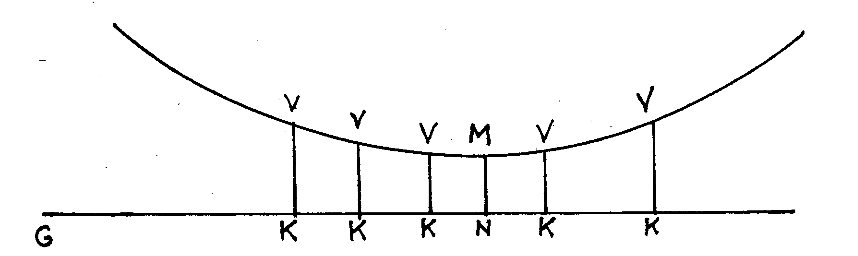
\includegraphics[width=.95\textwidth]{fig/Figure22}
\caption{}
\label{leasttime2A}
\vspace{-10pt}
\end{center}
\end{figure}
is equal to the line $QF$ in Figure~\ref{leasttime}, then $KV$ (in
Figure~\ref{leasttime2}) is equal to the difficulty of the path from
$C$ to $E$ through $F$; that is, when
$$GK = QF,$$
then 
$$KV =  (CF)\cdot h + (EF)\cdot r.$$

\subsection*{Note 14}
\label{cnm14}

To derive Leibniz's expression for $f$, we note that it follows from
Proposition I~47 in Euclid's {\em Elements} that
$$(CF)^2 =  (PC)^2 + (FP)^2 ,$$
and $PC= c$, while $FP = p-x$.  Substituting these expressions for
$CF$, $PC$, and $FP$ into the above equation, we get
\begin{eqnarray*}
f^2  & = & c^2 + (p-x)^2 \\
& = &  c^2 + p^2 - 2px + x^2.
\end{eqnarray*}
Taking the square root of each side of the equation, we get Leibniz's equation:
$$f = \sqrt{c^2 + p^2 - 2px + x^2}.$$

To derive Leibniz's equation for $g$, we again use Proposition I~47 in the {\em Elements}, according to which:
$$(EF)^2 = (EQ)^2 + (QF)^2.$$
$g$ is the line $EF$, $EQ = e$, and $QF = x$.  Therefore
$$g^2 = e^2 + x^2,$$
and, after we take the square root of each side,
$$g = \sqrt{e^2 + x^2}.$$

\subsection*{Note 15}
\label{cnm15}

Here is a derivation of Leibniz's expression for the differences of $\omega$:
\begin{eqnarray*}
d\omega & = & d(h\sqrt{l} + r\sqrt{m})\\
& = & d(h\sqrt{l}) + d(r\sqrt{m}) \mbox{\hspace{10ex} (addition rule)}\\
& = & hd(\sqrt{l}) + rd(\sqrt{m})  \mbox{\hspace{10ex} (constant multiple rule)}\\
& = & h\frac{dl}{2\sqrt{l}} + r\frac{dm}{2\sqrt{m}}  \mbox{\hspace{12.6ex} (root rule)}\\
& = & \frac{h\,dl}{2\sqrt{l}} + \frac{r\,dm}{2\sqrt{m}} \mbox{\hspace{15.1ex} (ordinary algebra)}
\end{eqnarray*}

\subsection*{Note 16}
\label{cnm16}

Here is a derivation of Leibniz's expression for the differences of $l$:
\begin{eqnarray*}
dl & = & d(c^2 + p^2 - 2px + x^2) \\
& = & d(c^2) + d(p^2) -d(2px) + d(x^2) \mbox{\hspace{5.55ex} (addition rule)}\\
& = & 0 + 0 -2p\,dx + d(x^2) \mbox{\hspace{15ex} (constant rules)}\\
& = & -2p\,dx + 2x\,dx \mbox{\hspace{21.15ex} (power rule)}\\
& = & 2dx(-p + x) \mbox{\hspace{23.78ex} (ordinary algebra)}\\
& = & -2dx(p-x) \mbox{\hspace{23.78ex} (ordinary algebra)}
\end{eqnarray*}

\subsection*{Note 17}
\label{cnm17}

Leibniz has just shown that 
\begin{equation} d\omega =  \frac{h\,dl}{2\sqrt{l}} + \frac{r\,dm}{2\sqrt{m}}  =0,
\end{equation}
and that 
\begin{eqnarray}
dl & = & -2dx(p-x),\\
dm & = & 2x\,dx,\\
\sqrt{l} & = & f,\mbox{ and}\\
\sqrt{m} & = & g.
\end{eqnarray}
Substituting the values from equations 2 through 5 into equation 1 gives
\begin{eqnarray*}
\frac{h(-2dx(p-x))}{2f} + \frac{r(2x\,dx)}{2g} & = & 0,\mbox{ and therefore}\\
-\frac{h(p-x)}{f} + \frac{rx}{g} & = & 0, \mbox{ and}\\
\frac{h(p-x)}{f} & = & \frac{rx}{g}.
\end{eqnarray*}
 
\subsection*{Note 18}
\label{cnm18}
This proportion is usually called {\em Snell's Law}, after Willebrord
Snellius, who discovered it in 1621.  At the time Leibniz wrote ``A
New Method," Descartes and Huygens had already published derivations
of it.  If we draw the line $UFT$ perpendicular to the line $QFP$ in
Figure~\ref{Snell},
\begin{figure}[htp]
\begin{center}
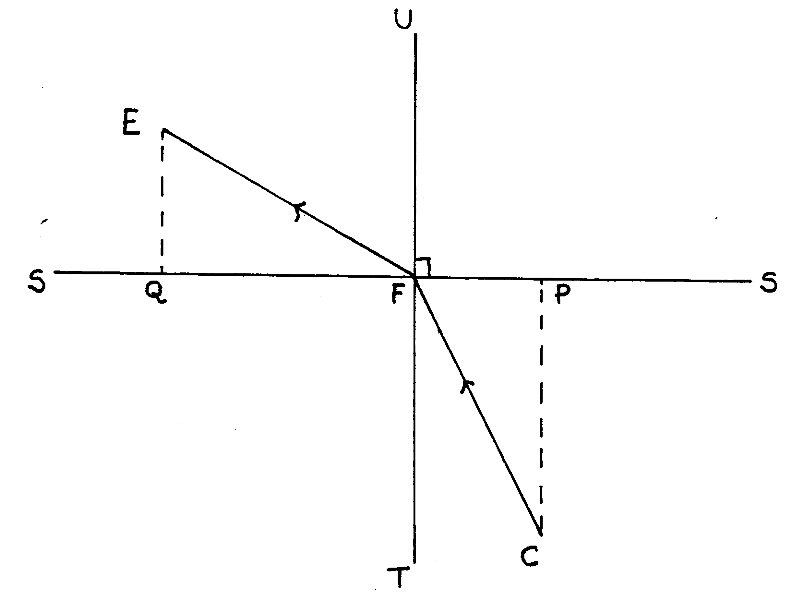
\includegraphics[width=.85\textwidth]{fig/Figure23}
\caption{}
\label{Snell}
\vspace{-10pt}
\end{center}
\end{figure}
 then the angle of incidence is $\angle CFT$ and the angle of refraction is $\angle EFU$.  We may assume that $FC = EF = 1$.  Then
$$\sin(\angle CFT) =  \sin(\angle FCP) = \frac{FP}{FC}= FP,$$
and
$$\sin(\angle EFU) =  \sin(\angle FEQ) = \frac{FQ}{EF} = FQ.$$

\subsection*{Note 19}
\label{cnm19}

In June of 1682 in an article titled ``The Unique Principle of Optics,
Catoptrics, and Dioptrics."  There he announces, without
demonstration, that his ``method of maxima and minima'' can be used to
prove Snell's law, and makes the following remark:
\begin{quote}
  We have therefore, by applying a single principle, reduced all the
  Laws of rays of light that have been proved by experience to pure
  Geometry and calculation; rightly considered, this principle comes
  from a final cause: for the ray of light going out from $C$ does not
  consider how it might most easily arrive at $E$, nor is it carried
  there by itself; but the Founder of things so created light, that
  this most beautiful outcome might arise from light's nature. And
  thus those who follow {\em Descartes} and reject {\em final causes}
  in Physics are very much in error (not to say anything more grave),
  since besides admiration of divine wisdom, final causes offer us a
  most beautiful {\em principle} for {\em discovering} the properties
  of those things whose inner nature is not yet so clearly known by us
  that we are able to use proximate efficient causes and explicate the
  machines which the founder has used to produce those effects and
  obtain his ends.  Hence we also understand that the meditations of
  the ancients in these matters too are not as contemptible as they
  seem now to some.
\end{quote}

\subsection*{Note 20}
\label{cnm20}

The curve 133 [Figure~\ref{locus2}] 
\begin{figure}[htp]
\begin{center}
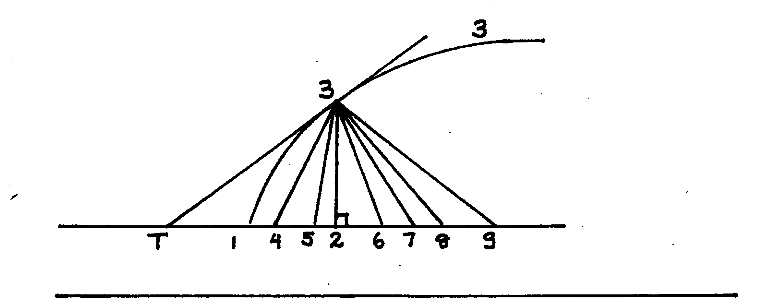
\includegraphics[width=\textwidth]{fig/Figure24}
\caption{}
\label{locus2}
\vspace{-10pt}
\end{center}
\end{figure}is the solution of a locus problem: if six points (here 4,
5, 6, 7, 8, and 9) are given, all on one straight line (here the line
T14526789), and if straight lines are drawn to each of these given
points from one point (here we draw the straight lines 34, 35, 36, 37,
38, and 39, all from the one point 3), such that all these drawn lines
are together equal to another given line (here the line $g$, so that
$34 + 35 + 36 + 37 + 38 + 39 = g$), then the one point (3) lies on the
locus in question (here the line 133).  If there were only two points,
4 and 5, instead of the six points Leibniz takes as given, then the
locus in question would be an ellipse whose foci are the points 4 and
5, and whose major axis is equal to $g$; for according to Proposition
52 of Book III of Apollonius' {\em Conics}, the sum of the two lines
from any point on an ellipse to the two foci is always equal to the
major axis.

Leibniz does not find an algebraic equation relating the abscissa and
ordinate of his locus, as Descartes does for Pappus' locus problem.
Instead, he finds a proportion giving the shape of the triangle (T23)
formed by the tangent, the ordinate, and the axis for any point 3;
once we have found the shape of the triangle (T23), we know where the
tangent must be.  Leibniz's proportion thus gives us a way to find the
tangent to the curve 133 at any point.

It is not necessary to go through a detailed derivation of Leibniz's
proportion, but for those who are interested, in the remainder of this
note we give a complete account of how to find the ratio of the line
23 to the line $T2$. We begin by noting that his ratio is equal to the
ratio of $d(23)$ to $d(12)$; for the triangle $3T2$ is similar to the
characteristic triangle, whose vertical side is equal to $d(23)$, and
whose horizontal side is equal to $d(12)$ [See Figure~\ref{locus2A}].
\begin{figure}[htp]
\begin{center}
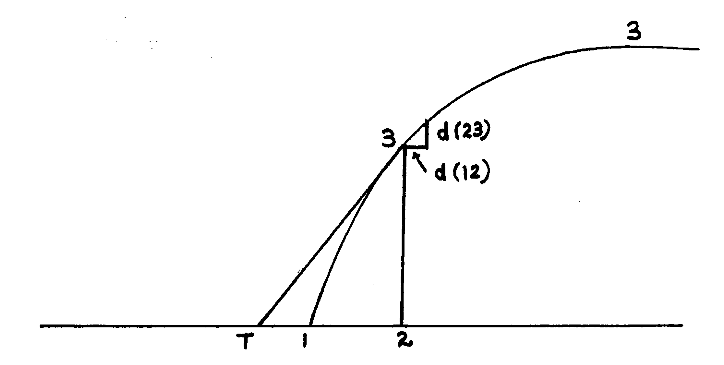
\includegraphics[width=\textwidth]{fig/Figure25}
\caption{}
\label{locus2A}
\vspace{-10pt}
\end{center}
\end{figure} Now to find the relation between these two differences,
we start by using the equation Leibniz uses to define the curve 13:
$$34 + 35 + 36 + 37 + 38 + 39 = g,$$
where $g$ is a constant.  We then find the difference of each side of
this equation, and use the addition and constant rules, to get the
differential equation
$$d(34) + d(35) + d(36) + d(37) + d(38) + d(39) = dg = 0.$$
But we want an equation for $d(12)$ and $d(23)$, not $d(34)$, $d(35)$,
etc.  We cannot immediately find an equation for $d(12)$ and $d(23)$,
but we can at least find an equation relating $d(23)$ and the
differences of some other lines on the axis besides 12.  To do this,
we use Proposition I~47 in Euclid's {\em Elements} to express each of
the lines 34, 35, etc., in terms of the line 23 and a line on the
axis: \setlength{\jot}{1ex}
\begin{eqnarray*}
(34)^2 & = & (42)^2 + (23)^2\\
(35)^2 & = & (52)^2 + (23)^2\\
(36)^2 & = & (26)^2 + (23)^2\\
\mbox{etc.} & & 
\end{eqnarray*}
\setlength{\jot}{\oldjot}
Therefore
\setlength{\jot}{1.5ex}
\begin{eqnarray*}
(34) & = & \sqrt{(42)^2 + (23)^2}\\
(35) & = & \sqrt{(52)^2 + (23)^2}\\
(36) & = & \sqrt{(26)^2 + (23)^2}\\
\mbox{etc.} & & 
\end{eqnarray*}
\setlength{\jot}{\oldjot}

Now we take the differences of all these equations, getting
\setlength{\jot}{1ex}
\begin{eqnarray*}
d(34) & = &d(\sqrt{(42)^2 + (23)^2})\\
d(35) & = &d( \sqrt{(52)^2 + (23)^2})\\
d(36) & = & d(\sqrt{(26)^2 + (23)^2})\\
\mbox{etc.} & & 
\end{eqnarray*}
\setlength{\jot}{\oldjot}

We then use the rules for the calculus to simplify all the differences
on the right sides of these equations.  For example, to find
$d(\sqrt{(42)^2 + (23)^2})$, we first set $a = (42)^2 + (23)^2$, so
that
$$d(34) = d(\sqrt{(42)^2 + (23)^2}) = d\sqrt{a}.$$
According to the root rule,
$$d(\sqrt{a}) = \frac{da}{2\sqrt{a}}.$$
To get an expression for $d(\sqrt{a})$ in terms of the lines (42) and
(23) and their differences, we need to find $da$:
\setlength{\jot}{1.5ex}
\begin{eqnarray*}
da & = & d((42)^2 + (23)^2) \\
& = & d((42)^2) + d((23)^2) \mbox{\hspace{10.9ex}(addition rule)}\\
& = & 2(42)d(42) + 2(23)d(23) \mbox{\hspace{6ex}(power rule).}
\end{eqnarray*}
\setlength{\jot}{\oldjot}
In the end, since we want to find the relation between $d(12)$ and
$d(23)$, we want to find an equation involving no other differences
besides these.  We therefore express 42 in terms of 12:
$$42 = 12 - 14,$$
and take differences
\begin{eqnarray*}
d(42) & = & d(12) -d(14) \mbox{\hspace{7.4ex} (addition rule)}\\
 & = & d(12). \mbox{\hspace{15ex} (constant rule)}
 \end{eqnarray*}
We may therefore substitute $d(12)$ for $d(42)$ in our expression for $da$:
\setlength{\jot}{1ex}
\begin{eqnarray*}
da & = & 2(42)d(42) + 2(23)d(23)\\
& = & 2(42)d(12) + 2(23)d(23).
\end{eqnarray*}
\setlength{\jot}{\oldjot}
Therefore
\setlength{\jot}{1.5ex}
\begin{eqnarray*}
d(34) & = & d(\sqrt{a})\\
 & = & \frac{da}{2\sqrt{a}}\\
 & = & \frac{2(42)d(12) + 2(23)d(23)}{2\sqrt{a}}\\
 & = & \frac{42}{\sqrt{a}}\,d(12) + \frac{23}{\sqrt{a}}\,d(23)\\
 & = & \frac{42}{34}\,d(12) + \frac{23}{34}\,d(23).
 \end{eqnarray*}
 \setlength{\jot}{\oldjot}
Similarly we can show that
\setlength{\jot}{2ex}
\begin{eqnarray*}
d(35)  & = & \frac{52}{35}\,d(12) + \frac{23}{35}\,d(23) \\
d(36)  & = & -\frac{62}{36}\,d(12) + \frac{23}{36}\,d(23) \\
d(37)  & = & -\frac{72}{37}\,d(12) + \frac{23}{37}\,d(23) \\
 &\mbox{etc.} &
\end{eqnarray*}
\setlength{\jot}{\oldjot}
(The minus signs in the expressions for $d(36)$, $d(37)$, etc., are
there because the points 6, 7 and so on are to the right of the point
2, and therefore $62 = 16 - 12$ and $d(62) = -d(12)$, etc.)

We now return to the original differential equation for the curve, and
substitute the expressions we have found for $d(34)$, $d(35)$, etc.:
\setlength{\jot}{2ex}
\begin{eqnarray*}
0 & = & d(34) + d(35) + d(36) + d(37) + d(38) + d(39) \\
  & = & + \frac{42}{34}\,d(12) + \frac{23}{34}\,d(23)\\
  & &  + \frac{52}{35}\,d(12) + \frac{23}{35}\,d(23)\\
  & &  -  \frac{62}{36}\,d(12) + \frac{23}{36}\,d(23)\\
  & & -  \frac{72}{37}\,d(12) + \frac{23}{37}\,d(23)\\
  &  & \mbox{\rule[-1em]{0em}{2.4em}etc.}   \\
  & = & \left(\frac{42}{34} + \frac{52}{35}  - \frac{62}{36} - \frac{72}{37} - \frac{82}{38} - \frac{92}{39}\right)d(12)  \\
  & & + \left(\frac{23}{34} + \frac{23}{35} + \frac{23}{36} + \frac{23}{37} + \frac{23}{38} + \frac{23}{39}\right)d(23) 
  \end{eqnarray*}
  \setlength{\jot}{\oldjot}

  Finally, we use this equation to solve for the ratio of $d(12)$ to
  $d(23)$ (that is, the ratio of $T2$ to 23). Subtracting the first
  term on the right from both sides of the equation gives: {\small
    $$ \left(\!\!- \frac{42}{34} - \frac{52}{35} + \frac{62}{36} +
      \frac{72}{37} + \frac{82}{38} + \frac{92}{39}\right)d(12) =
    \left(\frac{23}{34} + \frac{23}{35} + \frac{23}{36} +
      \frac{23}{37} + \frac{23}{38} + \frac{23}{39}\right)d(23).$$}
  Dividing both sides by $d(23)$ and
  $ \left(-\frac{42}{34} - \frac{52}{35} + \frac{62}{36} +
    \frac{72}{37} - \frac{82}{38} + \frac{92}{39}\right)$ gives:
  \begin{eqnarray*}
    \frac{d(12)}{d(23)} &  = &\frac{\frac{23}{34} + \frac{23}{35} +
                               \frac{23}{36} + \frac{23}{37} +
                               \frac{23}{38} + \frac{23}{39}}{
                               \left(-\frac{42}{34} - \frac{52}{35}  +
                               \frac{62}{36} + \frac{72}{37} +
                               \frac{82}{38} + \frac{92}{39}\right)}. 
  \end{eqnarray*}
This last equation is equivalent to the proportion Leibniz gives.

\subsection*{Note 21}
\label{cnm21}

That the same rule applies no matter how many points are given is
perhaps the reason Leibniz chooses to represent the points with
numbers rather than letters: there is no limit to the number of
symbols for numbers, and it may be easier to see the general pattern
in the rule when it is expressed in numbers.

\subsection*{Note 22}
\label{bdebeaune}
\label{cnm22}
 
The solution to De Beaune's problem is a logarithmic line, and Leibniz
seems to assume that readers are familiar with logarithmic lines.
Since most of us are not familiar with logarithmic lines, in this note
we give a brief introduction to them.

The note is divided into six
parts:
\begin{enumerate}
\itemsep0em
\item a definition of logarithmic lines;
\item differential equations for logarithmic lines;
\item natural logarithms;
\item the difference of $e^x$;
\item notation for logarithms; and
\item the difference of $\log x$, and finding differences of quantities involving logarithms.
\end{enumerate}

\subsubsection*{1. A definition of logarithmic lines}

An {\em arithmetic progression} is a series of quantities whose
successive differences are always equal.  The simplest example is the
series of numbers
$$1,\ 2,\ 3,\ 4, \ldots;$$
the difference of any two consecutive numbers in this series is always equal to 1.

A {\em geometric progression} is a series of quantities whose
successive ratios are always the same.  A simple geometric progression
is the series of numbers
$$2,\ 4,\  8,\ 16, \ldots;$$
any two consecutive numbers in this series are always in a two to one ratio.

A {\em logarithmic line}\label{logdef} may be defined as any line
such that any arithmetic progression of its abscissas corresponds to a
geometric progression of its ordinates.  See Figure~\ref{logs}.
\begin{figure}[htp]
\begin{center}
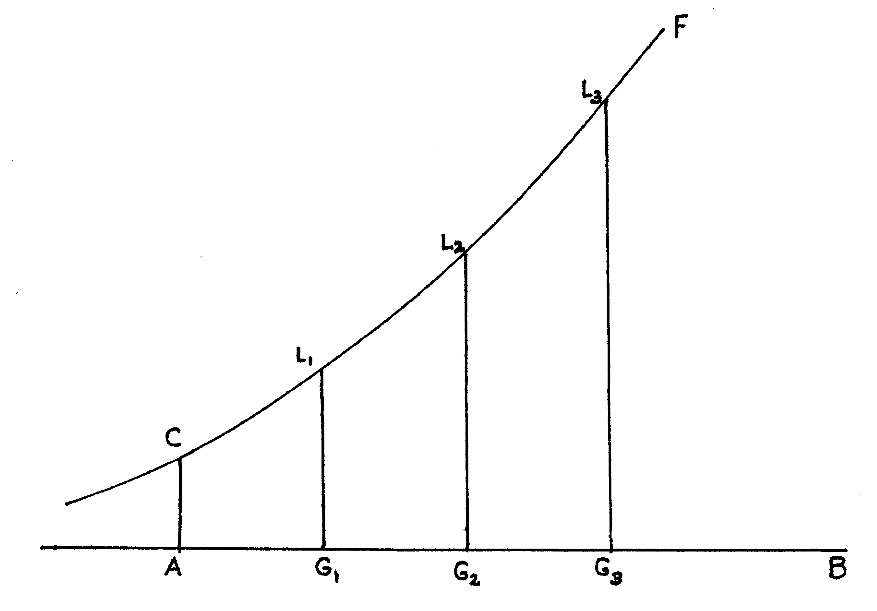
\includegraphics[width=\textwidth]{fig/Figure27A}
\caption{}
\label{logs}
\vspace{-10pt}
\end{center}
\end{figure}
  There the line $AB$ is an axis for the logarithmic line $CF$.  Therefore, if 
$$AG_1 = G_1G_2 = G_2G_3$$
(so that the abscissas $AG_1$, $AG_2$, $AG_3$ form an arithmetic progression),
 then the ordinates $AC$, $G_1L_1$, $G_2L_2$, and $G_3L_3$ of $CD$ form a geometric progression, that is
$$AC\!:\! G_1L_1 :: G_1L_1 \!:\! G_2L_2 :: G_2L_2 \!:\! G_3L_3.$$

If the ordinates of a logarithmic line are {\em numbers}, then the
abscissas of that same line are called the {\em logarithms} of those
numbers (with respect to that line).  For example, in
Figure~\ref{logs}, if
$$AG_1 = 1,\ AG_2 = 2,\ AG_3 = 3,\ \ldots,$$
and
$$G_1L_1 = 2,\ G_2L_2 = 4,\ G_3L_3 = 8,\ \ldots,$$
then 1 would be the logarithm of the number 2, 2 would be the
logarithm of the number 4, 3 would be the logarithm of the number 8,
and so on.  The series of logarithms,
$$1,\ 2,\ 3,\ \mbox{etc. }$$
is an arithmetic progression, and the series of corresponding numbers,
$$2,\ 4,\ 8,\ \mbox{etc. }$$
is a geometric progression.

Note that when we express numbers as powers, their exponents are
logarithms.  For example, we can express the geometric progression
$$2,\ 4,\ 8,\ \mbox{etc. }$$
as a progression of powers,
$$2^1,\ 2^2,\ 2^3,\ \mbox{etc. }.$$
The power of each number is its corresponding logarithm: the logarithm
of $2^1$ is 1, the logarithm of $2^2$ is 2, the logarithm of $2^3$ is
3, and so on.  In general if in Figure~\ref{logs} we assume that the
first ordinate $AC=1$, that $AG_1= G_1G_2= G_2G_3 \mbox{ etc.}$,\ and
we let
$$k = \frac{G_1L_1}{AC},$$
then because the ordinates $AC$, $G_1L_1$, $G_2L_2$ are in a geometric progression, 
$$k = \frac{G_1L_1}{AC} = \frac{G_2L_2}{G_1L_1} =  \frac{G_3L_3}{G_2L_2} =  \cdots.$$
Therefore
$$\begin{array}{lclcl}
G_1L_1 & = & k(AC )&  =&  k,\\
G_2L_2 &  = & k(G_1L_1) & = & k^2,\\
G_3L_3 &  = & k(G_2L_2) & = & k^3,\mbox{ etc.}
\end{array}$$
\setlength{\jot}{\oldjot}
\hspace{-.6em} If we denote the abscissa $AG$ by $x$ and the ordinates $GL$ by $w$, this means that when 
$$x = 1,\ 2,\ 3,\ \mbox{and so on},$$
then
$$w = k^1,\ k^2,\ k^3,\ \mbox{and so on;}$$
in other words, whenever $x$ is a positive integer, then
$$w = k^x.$$
The logarithm of $k^x$ is its exponent, $x$.

With a little more work we could show that whenever $x$ is a rational
number (that is, a fraction whose numerator and denominator are both
integers), then the same equation holds.  It is therefore reasonable
to assume that for {\em any} number $x$, \setcounter{equation}{0}
\begin{equation}
w = k^x.
\end{equation}
Equation~1 is an ordinary equation for the logarithmic line $CF$.
Note that it is in fact a {\em transcendent} equation, that is, an
equation of no definite degree (see page~\pageref{trandef} of ``A New
Method," and Note~9, above); for the variable $x$ is in an exponent.

The word {\em logarithm} comes from the Greek words
\foreignlanguage{greek}{l'ogos} ({\em ratio}) and
\foreignlanguage{greek}{>arijm'oc} ({\em
  number}): a logarithm is a number of a ratio.
In our example, the logarithm of $2$ is $1$, and $2$ is to $1$ in the
{\em simple} ratio of 2 to 1.  The logarithm of $4$ is $2$, and $4$ is
to $1$ in the {\em duplicate} ratio of $2$ to $1$:
$$4\!:\! 2 :: 2\!:\! 1.$$
The logarithm of $8$ is $3$, and $8$ is to $1$ in the {\em triplicate} ratio of $2$ to $1$:
$$8\!:\!  4 :: 4\!:\! 2 :: 2\!:\! 1.$$
In general, when the logarithm $AG$ is a whole number, it expresses
the degree to which the ratio of $GL$ to $AC$ is compounded of the
ratio of $2$ to 1.  Of course, $AG$ need not always be a whole number.



\subsubsection*{2. Differential equations for logarithmic lines}

Leibniz has shown that the line $WW$ (in Leibniz's Figure~\ref{debeaune2})
\begin{figure}[htp]
\begin{center}
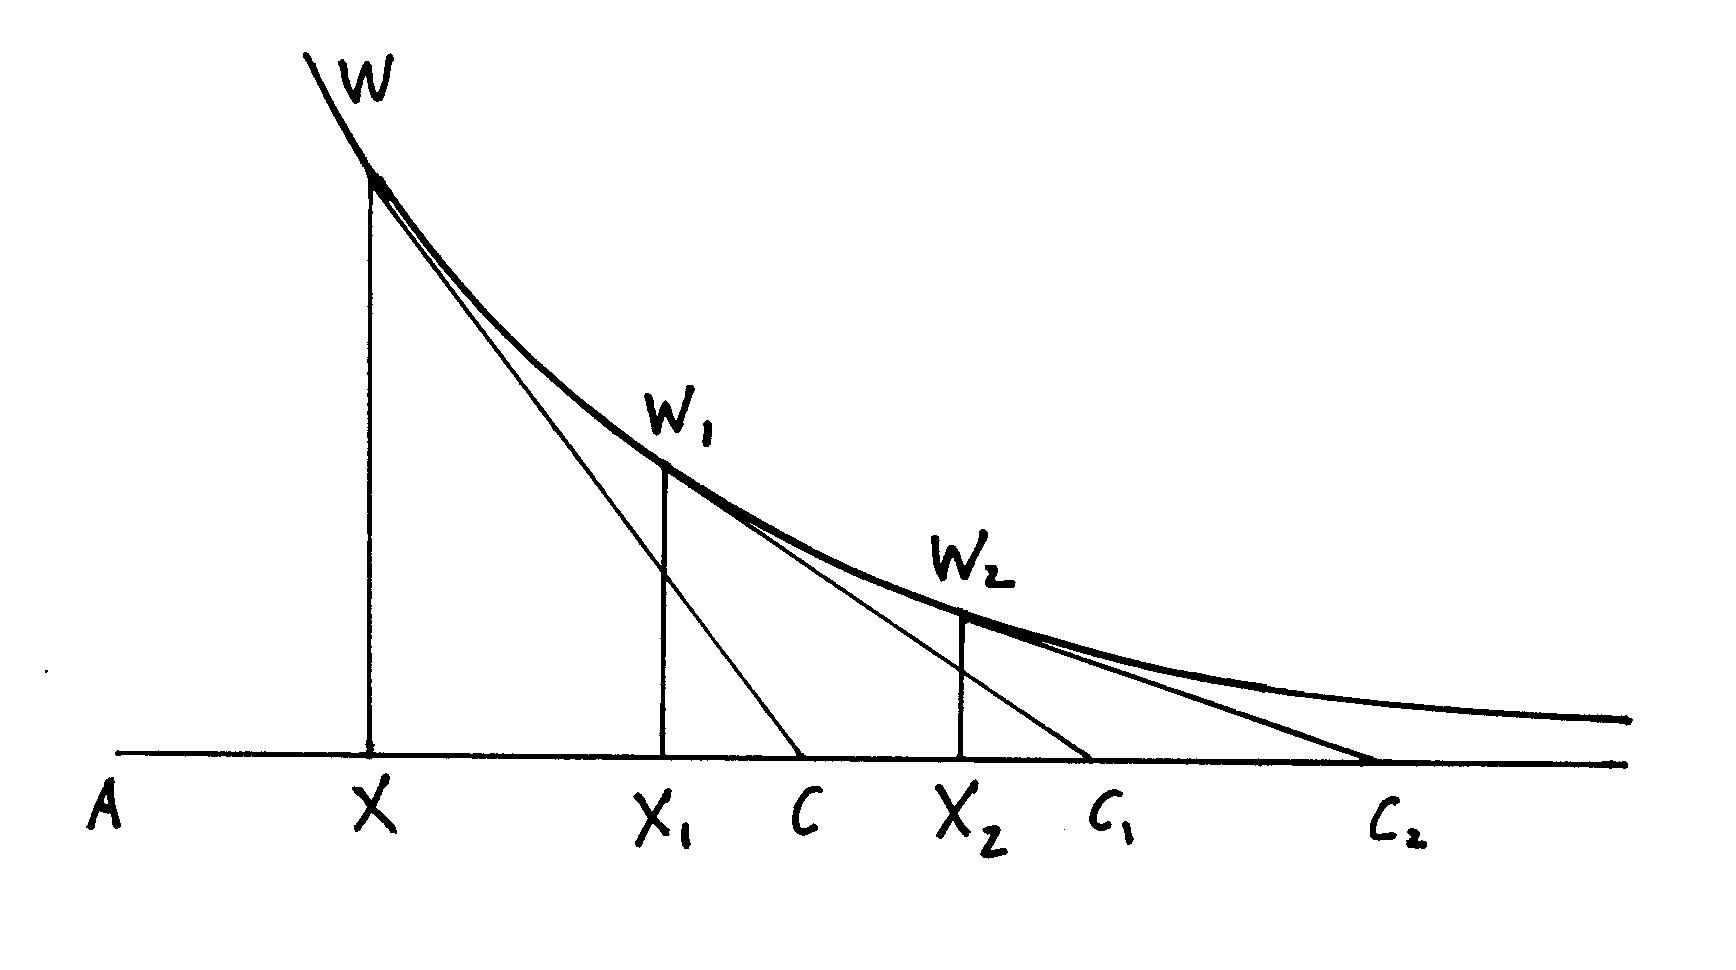
\includegraphics[width=.85\textwidth]{fig/Figure26A}
\caption{}
\label{debeaune2}
\vspace{-10pt}
\end{center}
\end{figure} 
which is a solution to De Beaune's problem is a solution to the differential equation
\begin{equation}
w = \frac{a}{b}dw,
\end{equation}
where $a = XC$ and $b= dx$ are constants.  He then claims that to say
that a line is a solution to equation~2 is equivalent to saying that
$WW$ is a logarithmic line; that is, that if a line is a logarithmic
line then it satisfies equation~2, and, conversely, that if a line
satisfies equation~2 then it is a logarithmic line.  In other words,
we have the following two theorems:

\begin{theorem}
If $WW$ is a logarithmic line, then
$$w= \frac{a}{b}dw,$$
where $a = XC$ and $b= dx$ are constants.
\end{theorem}

\begin{theorem}
If $WW$ is a line satisfying the differential equation
$$w=\frac{a}{b}dw,$$
where $a = XC$ and $b= dx$ are constants,
then $WW$ is a logarithmic line.
\end{theorem}

We will give a demonstration of Theorem~1 here, showing that any
logarithmic line is a solution of De Beaune's problem.  Theorem~2, the
converse of Theorem~1, is more difficult, and we do not demonstrate
it.  \vspace{\baselineskip}


\noindent {\bf Demonstration of Theorem~1:} Let $WW$ be a logarithmic
line whose ordinates $WX = w$ and whose abscissas $AX = x$.  We say
that $WW$ satisfies the differential equation~2:
$$w = \frac{a}{b}dw,$$
where $a$ is a constant equal to the distance $XC$ on the axis between
the ordinate $WX$ and the tangent $WC$ of the line $WW$, and $b=dx$,
the difference of the abscissas $AX$.

For let $AX$, $AX_1$, $AX_2$, and so on, be an arithmetic progression
of infinitely close abscissas, and let the infinitely small difference
between consecutive abscissas in this series be $b =dx$.  Then, since
$WW$ is a logarithmic line, the corresponding series of ordinates
$XW$, $X_1W_1$, $X_2W_2$, and so on, is a geometric series; that is,
there is one constant ratio $c$ such that
$$ c= \frac{w_1}{w} = \frac{w_2}{w_1} = \frac{w_3}{w_2}, \mbox{ etc.}$$
(Since $w_1$ is infinitely close to $w$, the quantity $c$ is infinitely close to $1$.)
Therefore
$$ w_1 = cw,\ w_2 = cw_1,\ w_3 = cw_2,\ etc.$$
Therefore, at the point $W$,
\begin{eqnarray*}
dw & = & w_1 - w\\
& = & cw -w\\
& = & (c-1)w,
\end{eqnarray*}
where $c-1$ is infinitely small.
 Likewise, at the point $W_1$,
 \begin{eqnarray*}
dw_1 & = & w_2 - w_1\\
& = & cw_1 -w_1\\
& = & (c-1)w_1.
\end{eqnarray*}

\hspace{-1em} A similar equation will hold for $W_2$, $W_3$, and, in
fact, for {\em any} point on the logarithmic line $WW$.  Therefore, no
matter what the value of the ordinate $w$,
$$dw = (c-1)w,$$
and therefore
$$\frac{w}{dw} = \frac{1}{c-1}$$
is constant.  

But, as Leibniz points out,
$$\frac{w}{dw} = \frac{XC}{b},$$ and therefore $XC$ must be constant
and the line $WW$ is a solution to De Beaune's problem.  Leibniz sets
$XC =a$, so that 
 \begin{figure}[htp]
   \begin{center}
     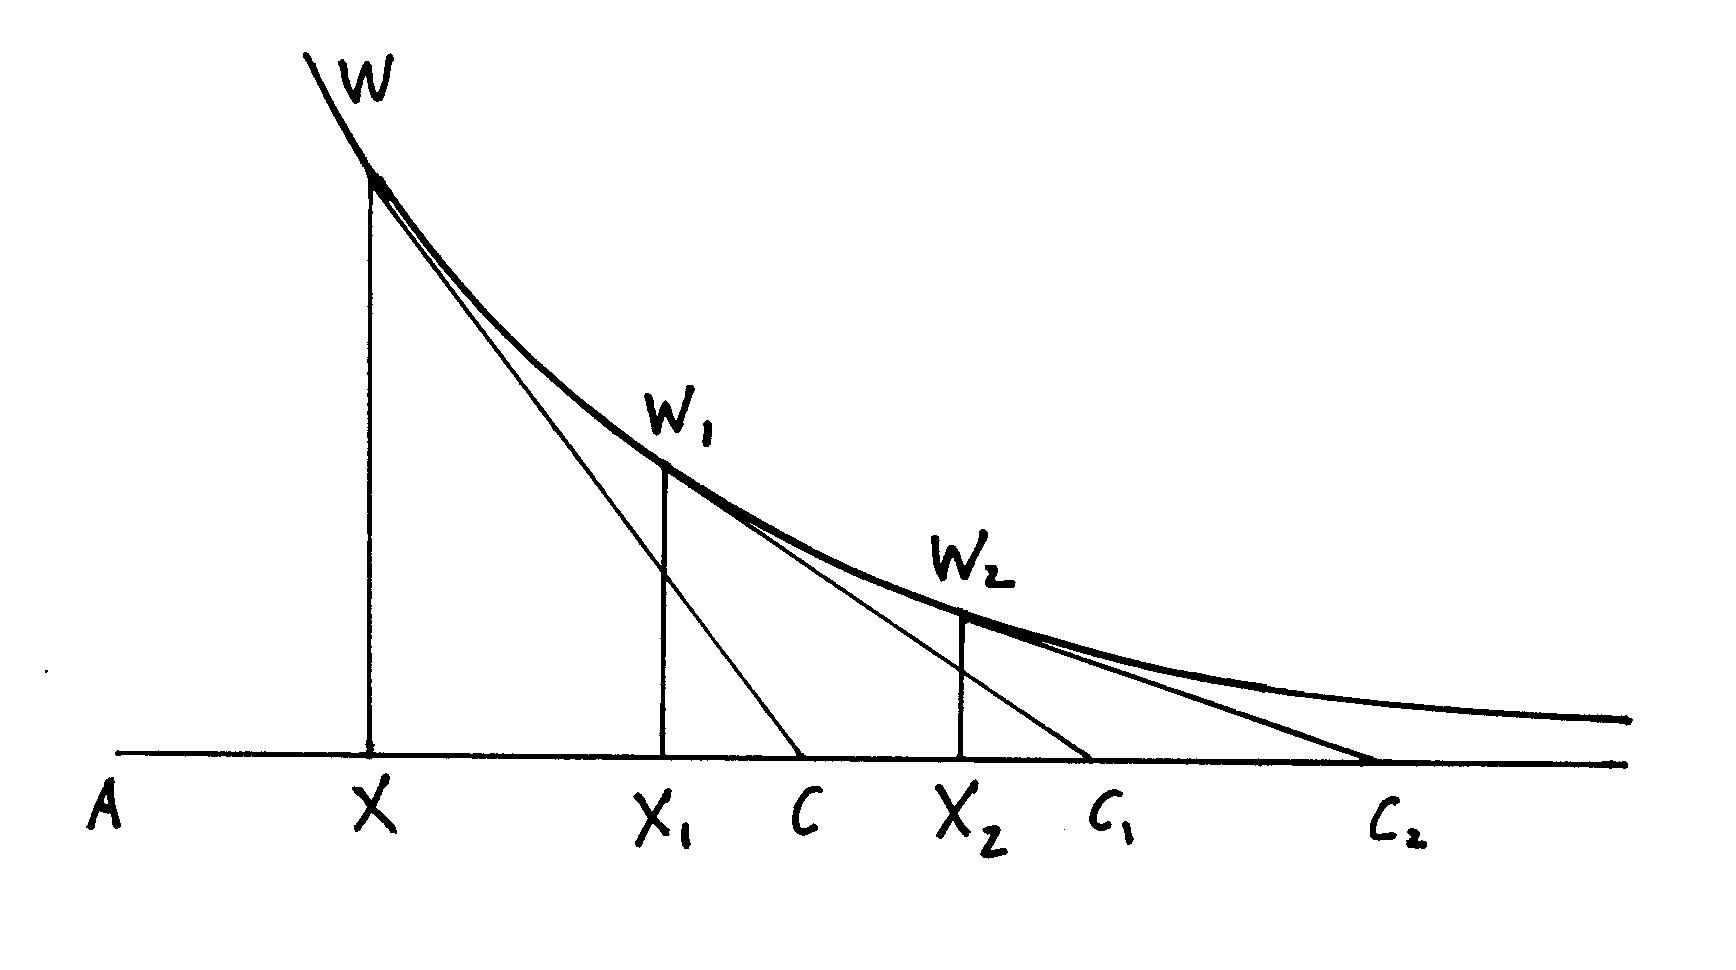
\includegraphics[width=.85\textwidth]{fig/Figure26A}
     \caption{}
     \vspace{-10pt}
   \end{center}
\end{figure} 
$$\frac{a}{b} = \frac{w}{dw},$$
and therefore
$$w = \frac{a}{b}dw.$$
This is equation~2.  Therefore if $WW$ is a logarithmic line whose
ordinates are $w$ and whose abscissas are $x$ then it satisfies the
differential equation
$$w = \frac{a}{b}dw,$$
where $a$ is a constant equal to $XC$, the distance on the axis
between the ordinate and the tangent, and $b$ is a constant $dx$ equal
to the difference of the abscissas $AX$.  \textsc{q.e.d.}
\vspace{.5\baselineskip}


\subsubsection*{3. Natural logarithms}

Both equation~1,\setcounter{equation}{0}
\begin{equation}
w= k^x,
\end{equation}
and equation~2,
\begin{equation}
w = \frac{a}{b}dw,
\end{equation}
contain arbitrary constants.  Equation~2 depends on $a$ ($b$ is equal
to $dx$, and in that sense is not arbitrary), while equation~1 depends
on $k$.  Different values of $a$ or of $k$ give equations
corresponding to different logarithmic lines.  The constant $a$ in
equation~2,
$$w = \frac{a}{b}dw,$$
is a constant of proportionality between the ordinates $w$ and the
differences of those ordinates, $dw$.  When $a$ is positive, a
positive value of $w$ corresponds to a positive value of $dw$, and
therefore the logarithmic line slopes upward, while if $a$ is
negative, a positive value of $w$ corresponds to a negative value of
$dw$, and therefore the logarithmic line slopes downward.
\begin{figure}[htp]
\begin{center}
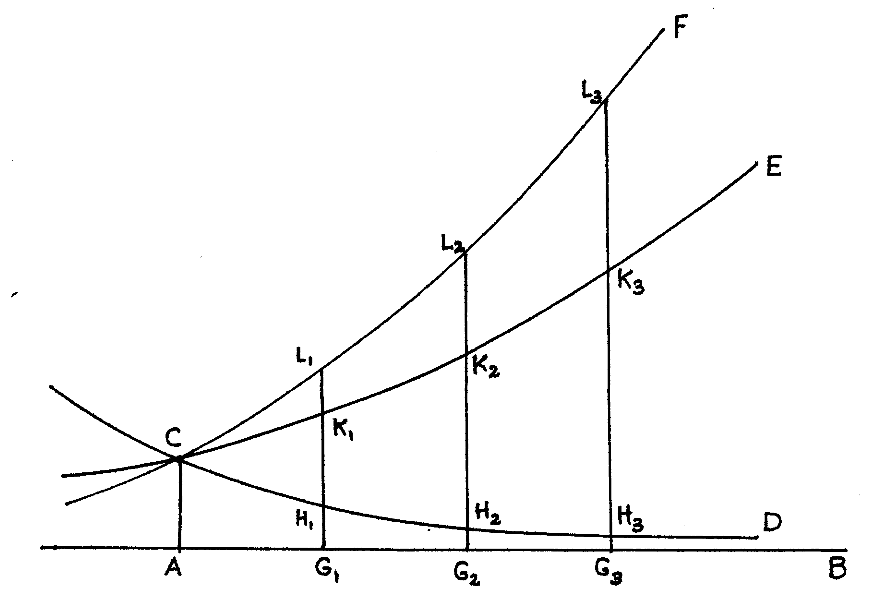
\includegraphics[width=\textwidth]{fig/Figure27}
\caption{}
\label{logs2}
\vspace{-10pt}
\end{center}
\end{figure} 
In Figure~\ref{logs2}, $a$ is positive for $CE$ and $CF$, while $a$ is
negative for $CD$.  When $a$ is positive, as it becomes larger, for
any given value of $w$, the differences $dw$ must be smaller.
Therefore, larger values of $a$ correspond to more gently sloping
logarithmic lines.  In Figure~\ref{logs2}, $CE$ has a larger value for
$a$ than $CF$.  The constant $k$ in equation~1,
$$w = k^x,$$ 
is the ratio of two ordinates corresponding to abscissas which are one
unit apart.  For example, in Figure~\ref{logs2}, if $AC = AG_1 =1$,
then $k=G_1H_1$ for the line $CD$, $k= G_1K_1$ for the line $CE$, and
$k=G_1L_1$ for the line $CF$.

When the constant $a=1$, then equation~2 becomes particularly simple:
$$w = \frac{1}{b}dw.$$
Substituting $dx$ for $b$, and solving for $dx$ gives:
\begin{equation}
\label{logdeq}
dx =  \frac{dw}{w}.
\end{equation}
In this case the line represented by equation~3 is said to be a {\em
  natural logarithmic line}, and the abscissas $x$ are said to be the
{\em natural logarithms} of the ordinates $w$.  If we use equation~1
instead of equation~3 to represent the natural logarithmic line, then
we denote by $e$ the value of $k$ that we need to use, so that
equation~1 becomes
 $$w = e^x$$\label{oeq}


 We have simply defined $e$ as the number such that $w = e^x$ is the
 equation for a natural logarithmic line; but we have as yet no notion
 of what the value of $e$ might be.  In fact it is difficult to
 determine an exact value for $e$, but the property of the tangents of
 the logarithmic line can help us limit the range of values that $e$
 might have, as shown in the following theorem.
\begin{theorem}
$2<e<4.$
\end{theorem}
\noindent {\bf Demonstration:}
See Figure~\ref{natlog2}. There $CL$ is again a natural logarithmic line whose ordinates $GL$ we
denote by $w$ and whose abscissas $AG$ we denote by $x$. The line
$TCM$ is tangent to $CL$ at $C$, and the line $CN$ is drawn parallel
to the axis $AG$.  Now if $AG=1$, then
$$GL = e^1 = e,$$
and thus $e$ appears in the diagram as the ordinate $GL$.
\begin{figure}[htp]
\begin{center}
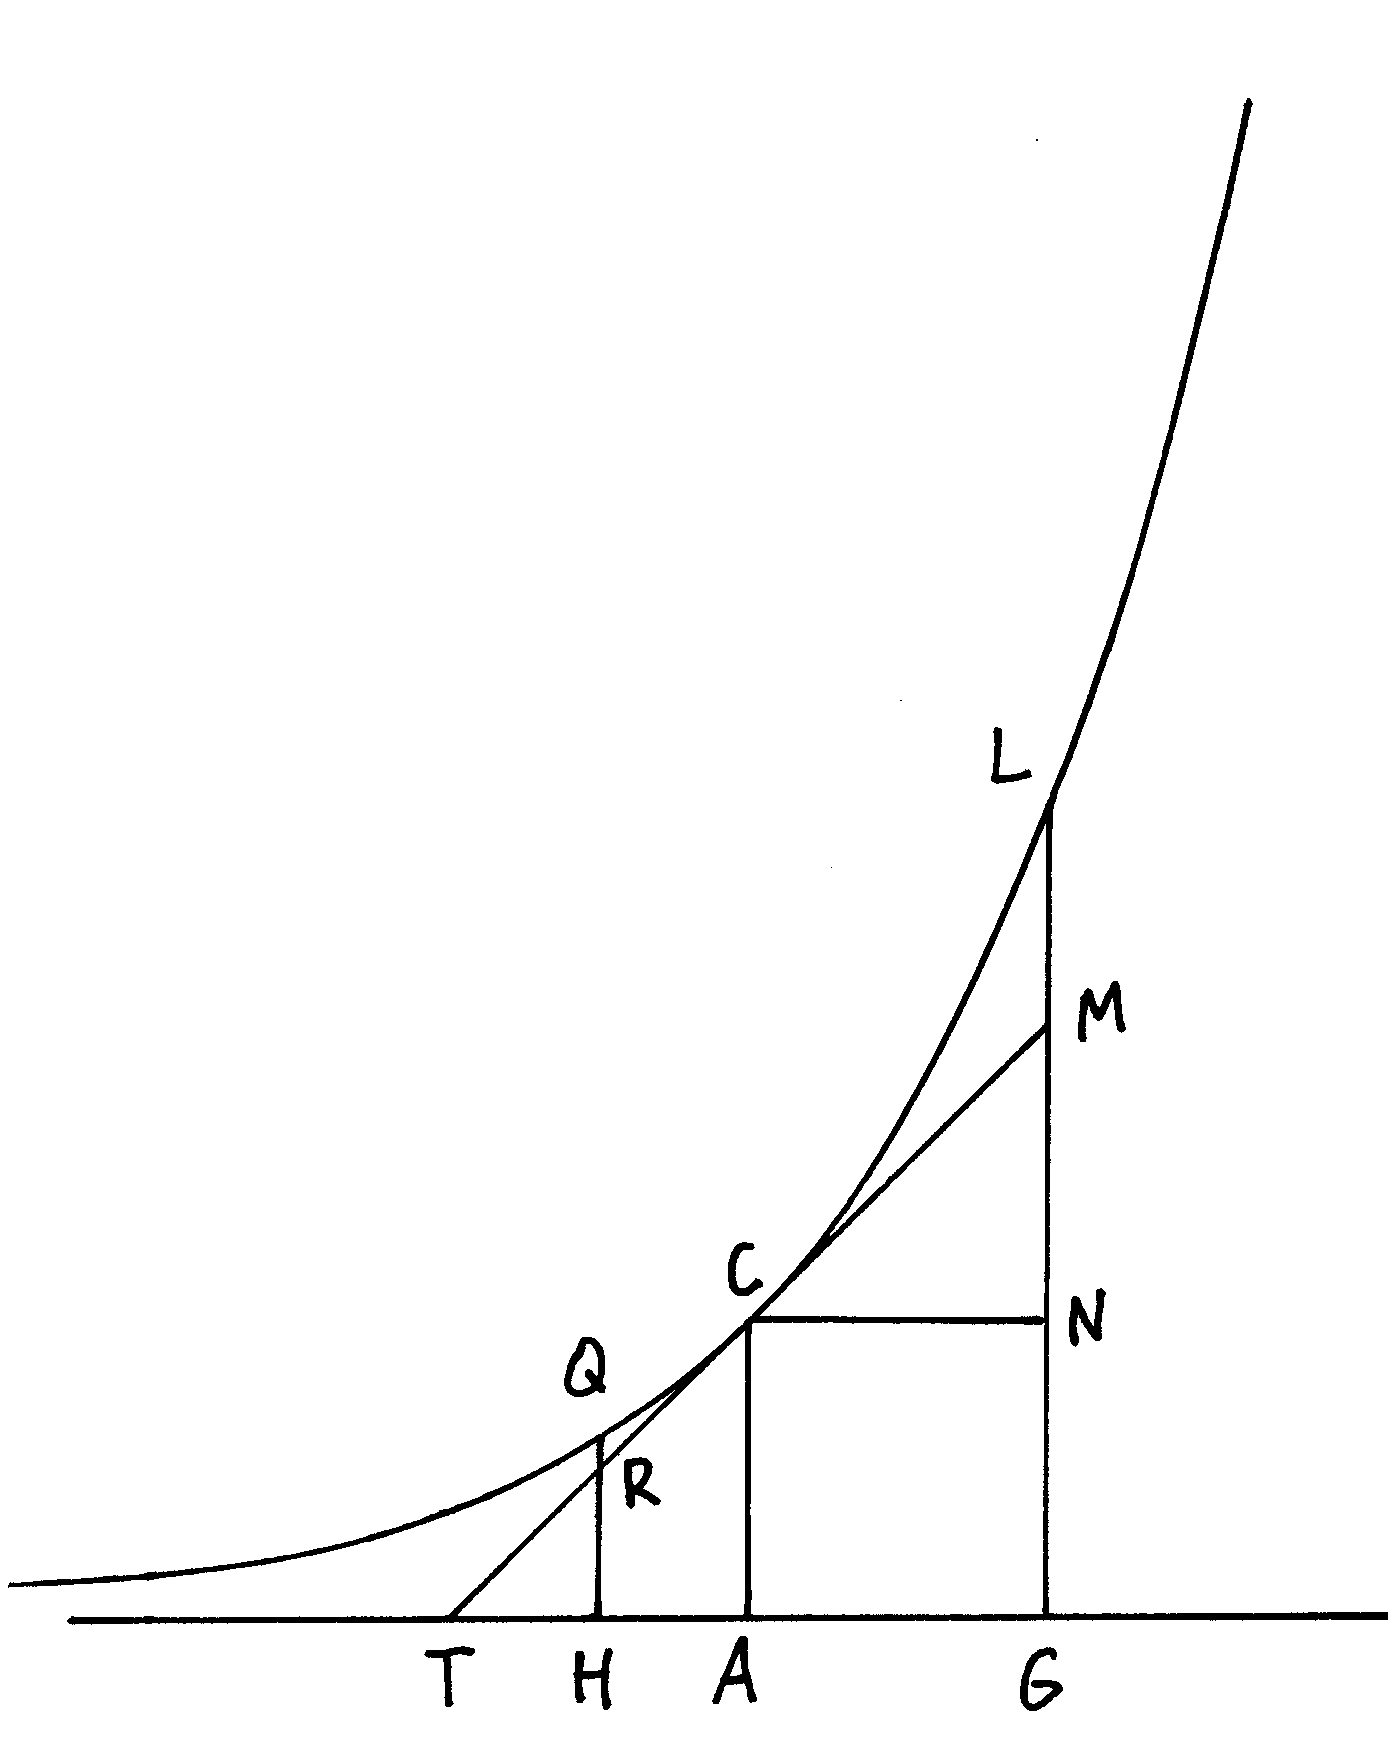
\includegraphics[width=.65\textwidth]{fig/Figure28A}
\caption{}
\label{natlog2}
\vspace{-10pt}
\end{center}
\end{figure}   

% Since $x=0$ at the point $A$, it follows that 
% $$AC = e^0 = 1.$$
% Since, as we saw above, $AT$ is also equal to 1, it follows that $AC = AT$ and therefore $MN = CN$.
% Now $1=AG = CN$, and therefore $MN=1$ and $GM =2$.  But since $TM$ is tangent to $CL$, 

Since $x=0$ at the point $A$, it follows that 
\[AC = e^0 = 1.\]
The triangle $TAC$ is similar to the characteristic triangle at the point $C$.  Therefore 
\[\frac{AC}{AT} =  \frac{dw}{dx},\]
and since $AC  =1$, it follows that 
\[\frac{1}{AT}= \frac{dw}{dx}.\]
But according to equation~3, above, 
\[\frac{dw}{dx} = w,\]
and at the point $C$, $w=1$.
Therefore 
\[\frac{1}{AT} = 1,\]
and so $AT =1$.
Likewise, the triangle $CNM$ is similar to the characteristic triangle at the point $C$, and therefore
\[\frac{MN}{CN} = \frac{dw}{dx} = 1,\]
and since $CN = AG =1$, it follows that $MN =1$.
Therefore $GM = GN + MN = AC + MN = 2$.  But since $TM$ is tangent to $CL$ \ldots
$$GL > GM,$$
and therefore 
$$e>2.$$  This is half of what the theorem asserts.

To show that $e<4$, we let $H$ be some point to the left of $A$, and draw the ordinate $HQ$, meeting the tangent $TC$ at $R$.    Let 
$$HA = \frac{1}{2},$$ so that 
$$-\frac{1}{2}$$
 is the value of the abscissa corresponding to the ordinate $HQ$; therefore 
$$HQ = e^{-\frac{1}{2}} = \frac{1}{\sqrt{e}}.$$
Since the tangent $TC$ falls below the logarithmic line $CL$, it follows that
$$RH <QH.$$
But 
$$RH = TH$$
(since triangle $THR$ is similar to triangle $TAC$),
and 
$$TH = TA - HA = \frac{1}{2}.$$
Therefore, the inequality $RH < QH$ becomes
$$\frac{1}{2}  < \frac{1}{\sqrt{e}},$$
and therefore
$$\sqrt{e} < 2$$
and 
$$e <4.$$ \textsc{q.e.d.}

The methods used in Theorem~3 can be generalized to find more exact approximations for $e$.

%The constant $e$ may be calculated approximately, and its value turns out to be about
%$ 2.71828$.

%Finally, before we turn to some problems, it is worth saying
% something about the etymology of the word {\em logarithm}.  The word
% {\em logarithm} comes from the Greek words
% \selectlanguage{greek}l'ogos\selectlanguage{english} ({\em ratio})
% and \selectlanguage{greek}>arijm'oc\selectlanguage{english} ({\em
% number}): a logarithm is a number of a ratio.  Suppose we are given
% a logarithmic line, satisfying equation~2:
%$$w = k^x,$$
%so that $x$ is the logarithm of $w$.
%If the logarithm of $w$ is 1, then $w = k^1 = k$ and $w$ is to 1 in
%the {\em simple} ratio of $k$ to 1; that is,
%$$w \!:\! 1 :: k \!:\! 1.$$
%If the logarithm of $w$ is 2, then $w = k^2$, and $w$ is to 1 in the
%{\em duplicate} ratio of $k$ to 1; that is,
%$$ w \!:\! k :: k \!:\! 1.$$
%If the logarithm of $w$ is 3, then $w = k^3$, and $w$ is to 1 in the
%{\em triplicate} ratio of $k$ to 1; that is,
%$$w \!:\! k^2 :: k^2 \!:\! k :: k \!:\! 1.$$
%In general, when the logarithm $x$ is a whole number, it expresses
% the degree to which the ratio of $w$ to 1 is compounded of the ratio
% of $k$ to 1.  Of course, $x$ need not always be a whole number.

\subsubsection*{4. The difference  of $e^x$}

Substituting the value $e^x$ for $w$ in the differential equation~3 (page~\pageref{logdeq}),
\setcounter{equation}{2}
\begin{equation}
dx = \frac{dw}{w}
\end{equation}
 gives us an equation for the differences of $e^x$:
$$\frac{d(e^x)}{e^x}   =  dx,$$
and therefore the differences of $e^x$
\begin{equation}
d(e^x) =  e^x\,dx.\label{dex}
\end{equation}
Equation~4 is the basic equation we use, along with the rules for the
calculus, to find differences of expressions involving $e$.  See the
examples in part~6 of this note, below.



\subsubsection*{5. Notation for logarithms}

If $x$ is the logarithm of $w$, so that $x$ represents the abscissa of
a logarithmic line and $w$ the corresponding ordinate, that is, if $x$
and $w$ are related by equation~1,
$$w = k^x,$$
then we write 
$$x = \log_kw.$$
This is simply a definition of a new symbol, $\log_k$.  For example, if $k=2$, then
\begin{eqnarray*}
\log_22 & = & 1,\\
\log_24 & = & 2,\\
\log_28 & = & 3, \mbox{ and so on,}
\end{eqnarray*}
since 
\begin{eqnarray*}
2 & = & 2^1 ,\\
4 & = & 2^2,\\
8 & = & 2^3, \mbox{ and so on.}
\end{eqnarray*}
The quantity $k$ is called the {\em base} of the logarithm.

When we are dealing with natural logarithms, so that equation~1 becomes,
$$w = e^x,$$
we simply write
$$x = \log w$$\label{nlognotation}
or
$$x = \ln w$$
for the natural logarithm\footnote{In contexts where numerical
  computation is important, $\log w$ often denotes the logarithm with
  base 10, that is,
$$\log_{10} w.$$
Since we will not be using logarithms for computation, $\log w$ will
always mean the {\em natural} logarithm of $w$ for us.} of $w$.


\subsubsection*{6. The difference of $\log x$, and finding differences of quantities involving logarithms.}

The differential equation~3,
$$dx = \frac{dw}{w},\label{deq}$$
where $x$ is the natural logarithm of $w$, may be used to find the
differences of quantities that are expressed in terms of logarithms,
as follows.  When $x$ is the natural logarithm of $w$, then
$$x = \log w,$$
and equation~3 may be rewritten as
\begin{equation}
d(\log w) = \frac{dw}{w} \label{dlog},
\end{equation}
that is, the difference of $\log w$ is equal to the difference of $w$ divided by $w$.

We can use formulas~4 (page~\pageref{dex}) and 5 to find sums and
differences of expressions involving natural logarithms and
exponentials, as the following examples show.

\begin{enumerate}
\item Let $z = e^{(2x-3)}$.  To find $dz$ in terms of $dx$.  Let
  $v= 2x-3$, so that $z = e^v$.  Therefore, by equation~4
  (substituting $v$ for $x$),
$$dz = d(e^v) = e^v\,dv;$$
and 
\setlength{\jot}{1.5ex}
\begin{eqnarray*}
dv & = & d(2x-3)\\
& = & d(2x) -d(3)\\
& = & 2\,dx.
\end{eqnarray*}
Therefore 
\begin{eqnarray*}
dz & = & e^v\,dv \\
& = & e^{(2x-3)}\,(2\,dx)\\
& = & 2e^{(2x - 3)}\,dx.
\end{eqnarray*}

\item Let $z = \log(5x^2 + 3).$ To find $dz$ in terms of $dx$.  Let
  $v= 5x^2 + 3$, so that $z= \log v$.  Therefore, by equation~5
  (substituting $v$ for $w$),
$$dz =  \frac{dv}{v};$$
and
\begin{eqnarray*}
dv &  = & d(5x^2 + 3)\\
& = & 5d(x^2) + d(3)\\
& = & 5(2x\,dx)\\
& = & 10x\,dx.
\end{eqnarray*}
Therefore
\begin{eqnarray*}
dz & = & \frac{dv}{v} \\
& = & \frac{10x\,dx}{5x^2 + 3}\\
& = & \frac{10x}{5x^2+ 3}\,dx.
\end{eqnarray*}

\item Let $z = \log^3(x-4)$, that is, $z = (\log(x-4))^3.$ To find
  $dz$ in terms of $dx$.  Let $v= \log(x-4),$ so that $z = v^3.$ Then,
  by the power rule,
$$dz = 3v^2dv.$$

Next, let $w = x-4,$ so that $v = \log w$.  Then, by equation~5,
$$dv = \frac{dw}{w}.$$

Finally, by the constant rule, 
$$dw = dx.$$

Putting all these equations together, we get
\begin{eqnarray*}
dz & = & 3v^2dv\\
& = & 3(\log(x-4))^2\left(\frac{dw}{w}\right)\\
& = & 3(\log(x-4))^2\left(\frac{dx}{x-4}\right).
\end{eqnarray*}

\setlength{\jot}{\oldjot}
\end{enumerate}

\subsubsection*{Problems about finding differences of exponentials and logarithms}

\label{pset4} Using the rules of the differential calculus, and
equations~4 (page~\pageref{dex}) and 5 (page~\pageref{dlog}), find the
following differences.
\begin{enumerate}
\itemsep0em
\item $$d(e^{(3x +1)}).$$
\item $$d(e^{(4x)} - 2e^{(2 - 3x)}).$$
\item $$d(\log(x^3 -2x)).$$
\item $$d(\log(x + 4) - \log^2 x).$$
\item $$d\left(\frac{\log(2x +3)}{e^x}\right).$$
\item $$d\left(\frac{e^{-x}}{\log 2x}\right).$$
\end{enumerate}
\label{edebeaune}

\setcounter{footnote}{0}
\setcounter{equation}{0}
\setcounter{figure}{0}

\section*{On Recondite Geometry and the Analysis of\\ Indivisibles and
  Infinites\marginnote{\normalfont\small\sffamily Note 1,
    p.~\pageref{crg1}}}
% \addcontentsline{toc}{section}{\protect\numberline{4}{Leibniz: On Recondite
\acl{Leibniz: On Recondite Geometry and the Analysis\\ of Indivisibles and Infinites}

\noindent {\large by Gottfried Wilhelm Leibniz}
\vspace{2ex}  

I am aware that some of the things I have published in these {\em
  Acts} for the advancement of geometry have been praised in no small
way by certain learned men, and indeed have been gradually put to use;
nevertheless, some things, either through the writer's fault or
through some other cause, have not been well enough understood, and
therefore I thought it worthwhile to add some things here that may
shed light on what I wrote earlier.  I have of course received Mr.\
Craig's {\em On the Measurement of Figures}, published last year in
London, from which it clearly appears that the author has made
advances that are not contemptible into the depths of geometry.  He
strongly approves of a distinction I have sometimes emphasized between
general and special measurements of figures, a distinction which he
says on page 1 has been very well observed recently by geometers, and
he rightly attributes the very many paralogisms of those who try to
prove the impossibility of a quadrature to the neglect of
this\marginnote{Note 2, p.~\pageref{crg2}} distinction.  He recognizes
with me that the figures that are commonly cast out of Geometry are
transcendent (page 26).\marginnote{Note 3, p.~\pageref{crg3}} He has
also greatly and humanely praised (pages 27 and 29) my Method of
Tangents, which I published in the {\em Acts} of October
1684;\footnote{The article ``A New Method for Greatests and Leasts, as
  well as for Tangents, which is not Hindered by Fractional or
  Irrational Quantities, and a Singular Calculus for these" (above,
  pages~\pageref{begnm}--\pageref{endnm}).}  he says that my method is
most extraordinary, and by means of it the method of measurements is
greatly helped, since it supplies the best remedy against
irrationalities.\marginnote{Note 4, p.~\pageref{crg4}} Nevertheless,
there are some things that I think it will not be useless or unwelcome
to call to his or others' attention.  Indeed, I do not know how it
happened that he believes that the man who wrote the paper in the {\em
  Acts} of May, 1684 (p. 233)\footnote{In May of 1684 Leibniz
  published the article ``On Finding Measurements of Figures," in
  which he first responded to Tschirnhaus.} retracted his opinion, and
although he had proposed, at the beginning of the {\em Acts} of
October, 1683, to give a demonstration that the quadrature of the
circle is in no way possible, afterwards, in May of the following
year, acknowledged that he had not yet demonstrated the impossibility
of a special quadrature.  Although the paper of October 1683 is by
Mr.\ D.\ T.,\footnote{Ehrenfried Walther von Tschirnhaus. The authors
  of articles in the {\em Acts of the Erudite} were often only
  identified by their (Latin) initials.} the paper of May 1684 is in
fact by me, and on the one hand I claimed that his method is mine, so
that I might not be accused of using something that belongs to someone
else, while on the other hand I amicably disagreed with the use that
Mr.\ D.\ T.\ put it to.  For he thought that the impossibility of any
definite quadrature followed from the impossibility of an indefinite
quadrature: but my constant position (already indicated when I
published the arithmetic quadrature\footnote{The article Leibniz
  refers to is ``On the True Proportion of a Circle to a Circumscribed
  Square," below, pages~\pageref{begtp}-\pageref{endtp}.} in the
second month of the first year of the {\em Acts}, 1682) had been that
the inference from the latter to the former is invalid.  To prove this
I gave an example (in the {\em Acts} of May, 1684) of a certain figure
that admits of a special quadrature but not a general quadrature, as I
tried to show there using Mr.\ D.\ T.'s own theorems, although I erred
in my calculation because I was in a hurry and certain of my method of
proof.  I will correct and explain this calculation later.  Mr.\ D.\
T.\ privately responded that he did not derive his method from mine,
but had come to it on his own and, as far as the objection was
concerned, that he could demonstrate the inference from indefinite to
definite quadratures, and this is what his method is especially good
for; indeed, he said my example rested upon a bad calculation.  I
indeed willingly admitted (in the {\em Acts} of December, 1684,
p. 587) that if he could demonstrate this inference, he would have
done what no one else had done yet; nevertheless, I continued to have
my doubts, and afterwards strengthened my example by a correct
calculation, which I will get to soon.  Moreover I have already had
this method for more than ten years, since the time we were together
in Paris and frequently spoke about geometric matters.  At that time
he was going in totally different directions, while I was already
quite familiar with how to apply general equations to express the
nature of the line sought, equations to be determined by the progress
of the calculation; this is the nerve of the method, and I had never
seen it published elsewhere.  But nevertheless I grant so much to both
his sincerity and his genius that I could easily believe that either
he came upon these things himself or at least no longer remembered on
what occasion the seeds of such meditations were sown, especially
since I know that he has come up with even more difficult things on
his own, and that we can look forward to many splendid and very
important things from his genius.

However since it is admitted that I made a mistake in the calculation
of the above-mentioned example, as I said, and I believe that Mr.\
Craig has used this error as an argument against Mr.\ D.\ T.\ (to whom
he attributes it) in order to refute the very method of indefinites, I
should correct the calculation.  Look at the {\em Acts} of the year
1684, page 239, where, in comparing the equation $4z^2-8hz$ etc.\ with
the equation $bz^2+caz$ etc., the terms without $z$ placed outside the
fraction in the latter equation should be multiplied by the
denominator of the fraction before the comparison is made, so that on
each side of the equation all the terms without $z$ are contained in a
single fraction.  And let $b=1$, which can always be done, and because
in the former equation the term $xz$ is entirely absent, $d$ becomes
$=0$ in the latter; and let the former (given) equation be divided by
$4$, and in the fraction of the latter (suppositional) equation let
both the numerator and the denominator be divided by $g$: thus both
the terms $z^2$ on each side, and the denominators of the fractions on
each side, agree.  When we compare the other terms, on account of the
term $z$, $c$ will become $= \frac{2h}{a}$; on account of $x^4$, $g$
will become $=\frac{1}{16}$; on account of $x^3$, $f$ will become
$= \frac{-1}{6a}$; and on account of $x$ in the denominator $f$ will
become $\frac{-h}{8z}$.  Therefore $h$ becomes $\frac{8}{6}$, that is
$\frac{4}{3}$, which is absurd, because $h$ is a given quantity.
Other absurdities also arise from the comparison, for both $f$ and $c$
become $=0$, contrary to what has already been concluded.

Further, to say something more useful here let us {\em reveal a source
  of Transcendent Quantities}, that is, a reason why some problems are
neither plane, nor solid, nor sursolid, nor of any definite degree,
but transcend every algebraic equation.  And at the same time we shall
show how it can be demonstrated without calculation that an algebraic
quadratrix for a circle or hyperbola is impossible.\label{logtrans}
For if such a line were given it would follow that by means of it an
angle or a ratio (or a logarithm) could be cut in a given ratio of a
line to a line, and this could be done by one general construction,
and consequently the problem of cutting an angle or finding an
arbitrary number of mean proportionals would be of a definite degree.
But for every different number of parts of an angle or every different
number of mean proportionals we need an algebraic equation of a
different degree, and therefore when the problem is understood to be
about any possible number of parts or mean proportionals, it is of
indefinite degree and transcends every algebraic equation.  Because
nevertheless such problems can be proposed in geometry---indeed,
they should be considered to be among its leading problems---and
because they are determinate, it is therefore obviously necessary to
admit into geometry those lines through which alone such problems may
be constructed; and since these problems can be described by an exact
and continuous motion, as is obvious in the case of the cycloid and
the like,\marginnote{Note~5, p.~\pageref{crg5}} they should indeed be
considered to be not mechanical, but geometric, especially since in
their usefulness they leave the lines of common geometry (if you leave
out the straight line and the circle) many parasangs behind, and have
properties of the greatest importance, and furthermore these
properties admit of geometric demonstrations.  {\em Therefore
  Descartes' error in excluding these lines from geometry was no less
  than that of the ancients}, who rejected solid or linear loci as
less geometric.\marginnote{Note 6, p.~\pageref{crg6}}

Moreover, because the method of investigating indefinite quadratures
or their impossibilities is for me only a special case (and indeed an
easier one) of a much greater problem, which I call the {\em inverse
  Method of Tangents},\marginnote{Note 7, p.~\pageref{crg7}} in which
the greatest part of transcendent geometry is contained, and because
if this problem can be solved algebraically, all sorts of discoveries
might be made, and because indeed I see nothing satisfactory about it
extant; for these reasons let me show how it can be done no less than
the indefinite quadrature itself can.  While before now algebraists
have taken letters or general numbers for the quantities sought, {\em
  I} have taken general or indefinite equations for the lines sought
in such transcendent problems; e.g., if the abscissa and ordinate are
$x$ and $y$, for me the equation of the line in question is
$$ 0 = a + bx + cy + exy + fx^2 + gy^2 \mbox{ etc.;}$$ 
by means of the proposed indefinite equation, which is in fact finite
(for it can always be determined how far up it has to go), I seek the
tangent of the line, and comparing what I find with the given property
of the tangents, I find out the value of the assumptive letters $a$,
$b$, $c$, etc.\ and to that extent define the equation of the line
sought;\marginnote{Note 8, p.~\pageref{crg8}} nevertheless sometimes
some things remain arbitrary, in which case innumerable lines can be
found that satisfy the problem, which is the reason why many, seeing
it afterwards, might think that the problem is not sufficiently
defined and is not in our power.  The same things can also be shown
through series.  I have many ways to make the calculation more
concise, which I save for another place.  But if the comparison does
not succeed, I declare that the line sought is not algebraic, but
transcendent.\marginnote{Note 9, p.~\pageref{crg9}}

If this is the case, to find out the {\em species of transcendence}
(for some transcendents depend on the general cutting of a ratio (or
logarithm), some on the general cutting of an angle (or on the arcs of
a circle), and some on other, more complex, indefinite questions) I
take in addition to the letters $x$ and $y$ a third letter such as
$v$, which signifies a transcendent quantity, and from these three I
form a general equation for the line in question;\marginnote{Note 10,
  p.~\pageref{crg10}} from this equation I seek the tangent of the
line by using the method of tangents I published in the {\em Acts} of
October, 1684, a method which is not hindered by transcendents.  Next,
comparing what I find with the given property of the tangents of the
curve, I discover not only the assumptive letters $a$, $b$, $c$, etc.,
but also the special nature of the transcendent.  Although it can
sometimes happen that we need to use more than one transcendent,
whenever their natures are different from each other, and
transcendents of transcendents are sometimes given, and, in general,
such things can go on indefinitely, nevertheless we can be content
with easier and simpler things.  And it is for the most part possible
to use special tricks, which I shall not give here, to make the
calculation shorter and reduce the problem to simple terms as far as
possible.  However, when this method is applied to tetragonisms, that
is, to finding quadratrices (for which a property of the tangents is
of course always given), it is easy not only to find out whether an
indefinite quadrature is algebraically impossible, but also how, after
the impossibility has been apprehended, a transcendent quadratrix can
be found.  No one else has done this yet, so that it seems to me that
I did not make an empty claim when I said that geometry is advanced by
means of this method immeasurably far beyond the boundaries set down
by {\em Vi\`{e}te} and {\em Descartes}, since in this way a certain
and general analysis extends to problems that are of no definite
degree and thus are not comprehended by means of algebraic equations.

Furthermore, because hardly anything\label{hardany} can be imagined
that is more useful, concise, and universal for treating transcendent
problems by calculation wherever measurements and tangents occur than
{\em my differential calculus or analysis of indivisibles and
  infinites}, of which only a small sample or corollary is contained
in my method of tangents, published in the {\em Acts} of October,
1684, and so greatly praised by {\em Mr.\ Craig}; and because {\em
  Mr.\ Craig} himself suspected that there is something deeper hidden
within this method, and consequently on page 29 of his book he tried
to derive from it Barrow's theorem (that the sum of the intervals
taken between the ordinates and perpendiculars of a curve and applied
to the axis is equal to half the square on the last
ordinate),\marginnote{Note 11, p.~\pageref{crg11}} although in
carrying out the derivation he missed his mark somewhat, which I do
not find surprising in a new method; for these reasons I judge that it
would be very welcome to him and to others, {\em if I disclose here an
  addition to something whose usefulness extends so broadly}.  For all
theorems and problems of this sort, which were rightly admired, flow
from it with such ease that now they no more need to be learned and
grasped than the many theorems of common geometry need to be learned
by heart by someone who grasps specious geometry.\marginnote{Note 12,
  p.~\pageref{crg12}} Therefore I proceed as follows in the
above-mentioned case.  Let the ordinate be $x$, the abscissa $y$
[Figure~\ref{barrow1}]
\begin{figure}[htp]
\begin{center}
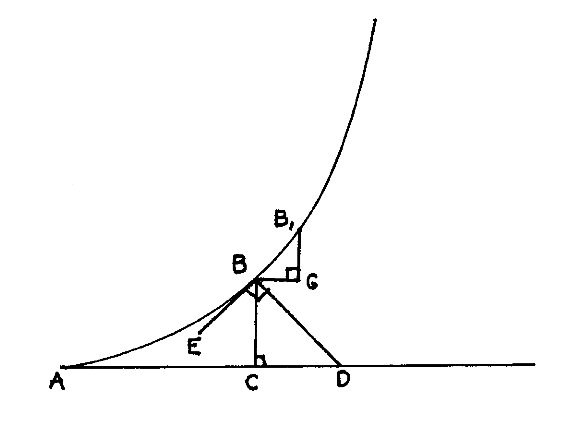
\includegraphics[width=.75\textwidth]{fig/Figure40}
\caption{our figure, not Leibniz's}
\label{barrow1}
\end{center}
\end{figure}  and let the
interval I mentioned between the perpendicular and the ordinate be $p$; it is
immediately obvious from my method that 
$$p\,dy = x\,dx,$$
which \marginnote{Note 13, p.~\pageref{crg13}}  {\em
Mr.\ Craig} also observed by using the same method; when this differential
equation is turned into an equation of sums, we get 
$$\int\!p\,dy = \int\!x\,dx.$$
 But \marginnote{Note 14, p.~\pageref{crg14}} it is obvious from the things I have set forth in the method
of tangents that 
$$d\left(\frac{1}{2}x^2\right) = x\,dx;$$
 and therefore correspondingly
$$\frac{1}{2}x^2 = \int\!xdx$$ 
(for sums and differences or $\int$ and $d$ are reciprocal for us just
as powers and roots are in common calculations).\marginnote{Note 15,
  p.~\pageref{crg15}} Therefore we have
$$\int\!p\,dy = \frac{1}{2}x^2,$$
which was what was to be demonstrated.  Now I prefer to use `$dx$' and
similar expressions rather than to substitute letters for them,
because the expression `$dx$' is a certain modification of the
expression `$x$,' and thus, by using this $dx$, we may ensure that,
when necessary, only the letter $x$ (together with its powers and
differentials) enters into the calculation, and the transcendent
relations between $x$ and something else are expressed.  In this way
it is possible to display transcendent lines by means of an equation;
for example, let $a$ be an arc and $x$ its versed sine; then
\marginnote{Note 16, p.~\pageref{crg16}}
 $$a = \int \!\frac{dx}{\sqrt{2x-x^2}},$$\label{lcircarc} \hspace{-.65em} and if $y$ is
the ordinate of the cycloid, then\marginnote{Note 17, p.~\pageref{crg17}}
 $$y = \sqrt{2x-x^2} +
 \int \!\frac{dx}{\sqrt{2x-x^2}},$$ which equation perfectly expresses
 the relation between the ordinate $y$ and the abscissa $x$, and from
 it all the properties of the cycloid can be demonstrated; and in this
 way analytic calculation is extended to those lines that have been
 thus far excluded for no greater reason than that they were believed
 not to admit of it; Wallis's interpolations and innumerable other
 things are also derived from this.

Finally, so that I may not seem to ascribe too much to myself or detract too
much from others, let me say in a few words what I think that I owe to the
mathematicians of our age who are distinguished in this sort of geometry.
{\em Galileo} and {\em Cavalieri} first began to uncover the very involved
arts of {\em Conon} and {\em Archimedes}.  But Cavalieri's geometry of
indivisibles belonged only to the infancy of a science in its rebirth.  Three
famous men helped more: {\em Fermat} by finding the method of greatest and
least lines, {\em Descartes} by showing the way to express the lines of common
geometry (for he excluded transcendents) through equations, and {\em Fr.\
Gregory of St.\ Vincent} by his many very splendid discoveries.  I add to
these the extraordinary rule of {\em Guldin} about the motion of the center of
gravity.  But these men also came to a stop within certain boundaries, which,
after opening a new approach, the renowned geometers {\em Huygens} and
{\em Wallis} crossed.  Indeed it is likely enough that Huygens's discoveries
gave to {\em Heurat}, and Wallis's gave to {\em Neil} and {\em Wren} (the men
who first demonstrated that curves are equal to straight lines), the
opportunity to make their own very beautiful discoveries, which nevertheless
takes nothing away from their well-deserved praise.  The Scot {\em James
Gregory} and the Englishman {\em Isaac Barrow}, who wonderfully enriched the
science with splendid theorems of this kind, followed these men.  Meanwhile
{\em Nicolas Mercator} of Holstein, a mathematician and a most outstanding
one, is the first I know to have given a quadrature by means of an infinite
series.  But a geometer of most profound genius, {\em Isaac Newton}, not only
made the same discovery on his own, but also solved the problem by a certain
universal method; if Newton were to publish his thoughts, which I understand
he has thus far suppressed, he would undoubtedly open up for us new ways to
make science grow and become more concise.

It happened that while I was still a beginner in these studies, from
one aspect of a certain demonstration about the magnitude of a
spherical surface, a great light suddenly dawned on me. For I saw that
in general the figure made from the perpendiculars to a curve, drawn
ordinatewise to the axis (in the case of the circle, the figure made
from the radii) is proportional to the surface of the solid that
arises from the rotation of the figure about the axis.\marginnote{Note
  18, p.~\pageref{crg18}} Wonderfully delighted with this first
theorem (since I did not know that something similar had been noticed
by others), I immediately invented the triangle that in any curve I
called the characteristic triangle, whose sides were indivisibles (to
speak more accurately, infinitely small) or differential quantities;
by using it I immediately composed innumerable theorems with no
trouble, part of which I afterwards found in {\em Gregory} and {\em
  Barrow}.  And I was not yet using the true algebraic calculus; when
I started to use it I soon found my arithmetic quadrature and many
other things.  But somehow the algebraic calculus did not satisfy me
in this business, and I was forced to show many things by moving
figures around that I wanted to show by analysis, until at last I
found the true supplement to algebra for transcendents, namely, my
calculus of the indefinitely small, which I also call differential, or
summing, or tetragonistic, and quite appropriately (if I am not
mistaken) the {\em Analysis of indivisibles and infinites}; once I had
discovered this calculus, everything I myself had previously admired
in this area seemed to be child's play.  It not only led to marked
abbreviations, but also made it possible to put together the very
general method that I set forth above, whereby quadratrices or other
lines, algebraic or transcendent,\label{quadothalg} are determined as
far as possible.  Before I finish, let me give a warning: in
differential equations, such as
$$a= \int\!\frac{dx}{\sqrt{1-x^2}},$$\label{rgcircarc}%
let no one heedlessly neglect the $dx$ itself because it can be
neglected in the case where the $x$'s themselves are assumed to grow
uniformly.  For most err in just this way and prevent themselves from
advancing further because they do not let indivisibles like $dx$ keep
their universality (so that any kind of progression might be taken for
the $x$'s themselves), although innumerable transfigurations and
equipotencies of figures may arise from this very
thing.\marginnote{Note 19, p.~\pageref{crg19}}

After I had already finished writing this little article, the things
that Mr.\ D.\ T.\ shared in the {\em Acts} of March of this year on
page 176 came into my hands, where he proposed some elegant questions
that are worthy to be solved.\marginnote{Note 20, p.~\pageref{crg20}}
And I see that the line $ACI$ (Figure~\ref{Tschirn1})
\begin{figure}[p]
\begin{center}
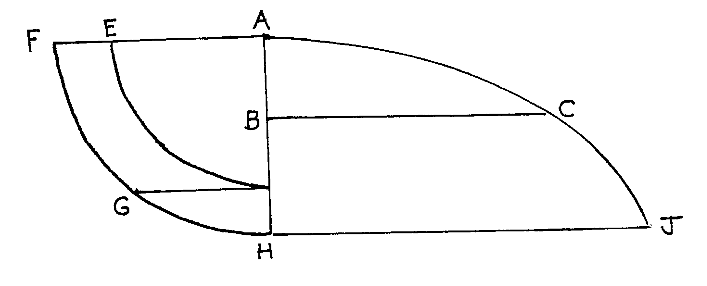
\includegraphics[width=\textwidth]{fig/Figure54}
\caption{Leibniz's figure}
\label{Tschirn1}
\end{center}
\end{figure}  
is one of the lines of
sines, and the rectangle formed by $AH$ and $GD$ is equal to the space $ABCA$.  And in
Figure~\ref{Tschirn2},
 \begin{figure}[p]
\begin{center}
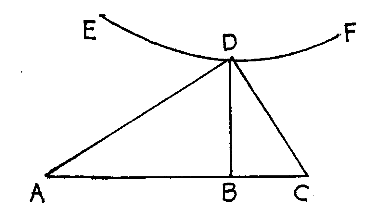
\includegraphics[width=.6\textwidth]{fig/Figure55}
\caption{Leibniz's figure}
\label{Tschirn2}
\end{center}
\end{figure} if the solid formed by the square on $BC$ and $BD$ (or
$x$) should always be equal to the given cube from $a$, I see that the
paraboloid whose equation is $4a^3 y^2 = 25x^5$ satisfies the problem.
It is possible to determine something similar for other powers.  But
if $AD$, $DB$, $BC =$ the given cube, it reduces to the squaring line
of the figure the value of whose ordinates is $ax^3$ divided by
$\sqrt{a^6- x^6}$; and in general the problem of finding the line with
a given relation between the straight lines $AB$, $BC$, $CD$, $AD$,
$DB$ in the said Figure~\ref{Tschirn2} coincides with a problem of
finding quadratures.  But if a fixed point $L$ is taken on the line
$AC$ new relations of a different nature arise (for example, the ratio
between $LC$ and $CD$ may be given), and this problem likewise admits
of a solution.

\setcounter{equation}{0}

\section*{Notes on Leibniz's ``On Recondite Geometry"}
%\addcontentsline{toc}{section}{\protect\numberline{5}{Notes on
\acl{Notes on Leibniz's ``On Recondite Geometry"}

Leibniz published this paper in the {\em Acts of the Erudite} in June
of 1686, about a year and half after ``A New Method."  We have
translated it from the Latin text in Gerhardt's edition, Volume V,
pages 226--33.

\subsection*{Note 1}
\label{crg1}

In ``A New Method," Leibniz shows how, given a relation between
quantities, we can find a {\em differential equation} relating their
differences, and how we can use this differential equation to solve
geometric problems by finding greatest and least ordinates and finding
tangents (see page~\pageref{nmdiffeq} of ``A New Method" and
page~\pageref{diffeq} of our notes).  ``On Recondite Geometry" treats
the inverse problem: Leibniz shows how, given a differential equation
relating the differences of some quantities, we can (in some cases)
find the relation between the quantities {\em themselves}; and he
shows how we can use this relation between the quantities to solve a
geometric problem: the problem of finding the measurements of
curvilinear figures (that is, lengths, areas, and volumes).  To solve
the problem of finding the relation between quantities with a given
differential equation, Leibniz introduces into his calculus a new
operation, ``summing," represented by a new symbol, $\int$.

\subsection*{Note 2}
\label{crg2}

\subsubsection*{The Measurement of Figures}

In Proposition I~45 of the {\em Elements}, Euclid shows how to find a
rectangle equal to any given {\em rectilinear} figure.  To find a
rectangle equal to a given {\em curvilinear} figure is a problem of
quadrature, also called ``tetragonism."  For example, to find the
quadrature of a circle, to ``square a circle," is to find a square
equal to the circle.  This is not a problem new to Leibniz:
Archimedes, for one, offers a demonstration that ``the area of any
circle is equal to a right-angled triangle in which one of the sides
about the right angle is equal to the radius, and the other to the
circumference of the circle."\footnote{See Archimedes' {\em
    Measurement of the Circle}, Proposition~1.}

\subsubsection*{General and Special Measurements of Figures}



In this passage, Leibniz distinguishes a general (or indefinite)
quadrature from a special (or definite) quadrature.  To find a special
(that is, specific) quadrature is to find the sides of the rectangle
equal to a single, constant area.  An example of a problem of special
quadrature is shown in Figure~\ref{fig25a}:
\begin{figure}[htp]
\begin{center}
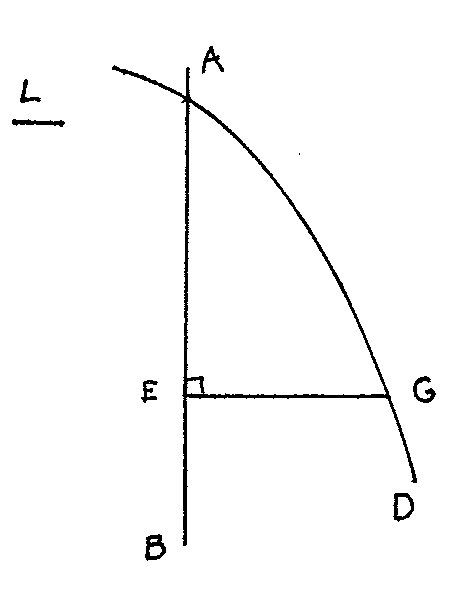
\includegraphics[width=.5\textwidth]{fig/Figure29A}
\caption{}
\label{fig25a}
\end{center}
\end{figure} 
given a curve $AD$ with axis $AB$ and ordinate $EG$, and one side $L$
of a rectangle, the problem is to find the other side $M$ of the
rectangle which will enclose an area equal to the curvilinear figure
$AEG$.
	
The problem of a general (or indefinite) quadrature is to find the
rectangles that enclose a varying or variable area.  For example,
Figure~\ref{fig25b},
\begin{figure}[htp]
\begin{center}
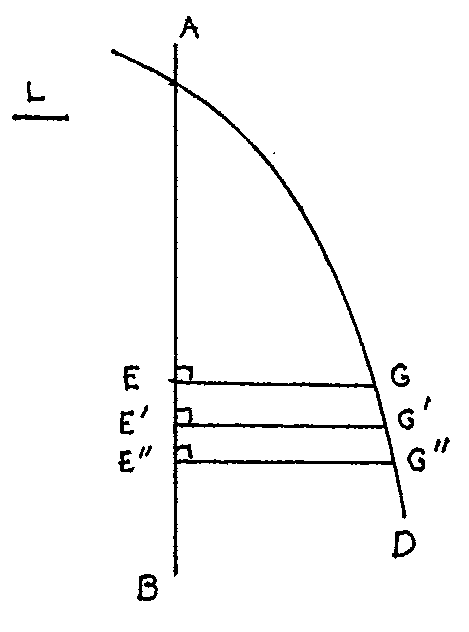
\includegraphics[width=.5\textwidth]{fig/Figure29B}
\caption{}
\label{fig25b}
\end{center}
\end{figure} 
given a curve $AD$ with axis $AB$ and ordinate $EG$, and one side $L$
of the rectangle, the problem is to find the second sides $M$, $M'$,
$M''$, etc., of the rectangles equal to the curvilinear areas $AEG$,
$AE'G'$, $AE''G''$, etc.
 
Now to represent all these lines in a single figure
(Figure~\ref{quadratrix}), let $EF = M$, $E'F' = M'$, $E''F'' = M''$,
etc.
\begin{figure}[htp]
\begin{center}
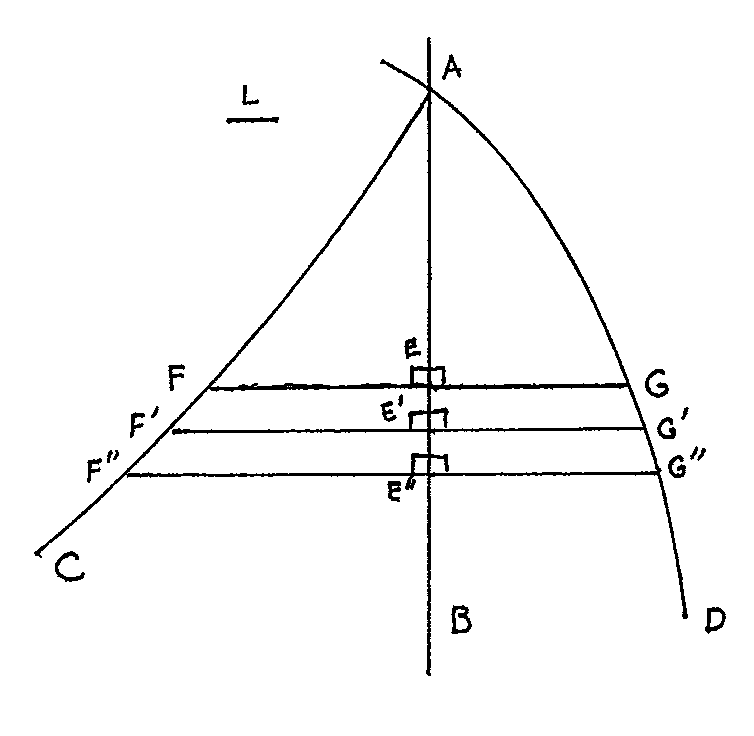
\includegraphics[width=.75\textwidth]{fig/Figure29C}
\caption{}
\label{quadratrix}
\vspace{-10pt}
\end{center}
\end{figure} 
Then if we have found all possible second sides $M$, $M'$, etc., the
points $F$, $F'$, etc., will trace out a curved line $AFC$, such that
for any ordinate $EG$ the rectangle on $EF$ and $L$ is equal to the
curvilinear area $AEG$.  Therefore to find the line $AFC$ is
equivalent to finding the quadrature of all possible areas $AEG$, that
is, to finding a general quadrature.  The curve $AFC$ thus gives us a
way to measure not just a single area, but the variable area $AEG$,
which changes as the ordinate moves.  The original curve $AGD$ is
called the {\em quadranda}, that is, the ``curve to be squared", while
the curve we find, $AFC$, is called the {\em
  quadratrix}\label{quaddef}, that is, the ``squaring curve," because
it lets us find a square equal to the area $AEG$ by finding a square
equal to the rectangle on $FE$ and $L$.

\subsection*{Note 3}
\label{crg3}
The term ``transcendent'' (also ``transcendental") is opposed to
``algebraic." It means: transcends finite algebraic operations. The
term may be applied to a number or a curve. An algebraic
number is one that is a solution to an algebraic equation with one
variable, that is, an equation of the form
\begin{align*}
a_{n}x^n+a_{n-1}1x^{n-1}+\cdots+a_1x+a_0=0
\end{align*}
where $n$ is a natural number and $a_0, a_1, \dotsc$ are integral coefficients.
For example,
$$3x^2 + 2x -5  = x^9 - 3x^5$$
is an algebraic equation, and so its solutions are algebraic numbers.


A transcendent curve is one that cannot be expressed by an algebraic
equation.  While a number is defined by an equation in one variable, a
curve is defined by an equation in two variables.  Such an equation is
algebraic when it is a polynomial in two variables with any
coefficients, that is, when it is of the form
\begin{align*}
0 & = a_{n,m}x^ny^m + a_{n-1,m}x^{n-1}y^m + \cdots + a_{1,m}xy^{m} + a_{0,m}y^m\\
&+ a_{n,m-1}x^ny^{m-1} + a_{n-1,m-1}x^{n-1}y^{m-1} + \cdots + a_{1,m-1}xy^{m-1} + a_{0,m-1}y^{m-1} \\
& +\cdots \\
&+ a_{n,1}x^ny + a_{n-1,1}x^{n-1}y+ \cdots + a_{1,1}xy+ a_{0,1}y \\
& +a_{n,0}x^n + a_{n-1,0}x^{n-1}+ \cdots + a_{1,0}x+ a_{0,0}.
\end{align*}
where $n$ and $m$ are natural numbers and the numbers $a_{i,j}$ (for
all values of $i$ between 0 and $n$ and all values of $j$ between 0
and $m$) could be any numbers.

For example,
 $$3x^2 - 2y^2 + 2xy - 7x + 1 = 0$$
is an algebraic equation corresponding to an algebraic curve.  

Descartes called transcendent curves ``mechanical,'' as opposed to
``geometrical'', indicating thereby that, although one can construct
mechanical devices by which such a curve may be traced, there seems to
be no rigorous determinable rule that relates a given abscissa to its
corresponding ordinate. Such curves thus seem to elude analysis. There
are many transcendent curves: the sine curve, along with the other
trigonometric curves, the logarithmic curve, the logarithmic spiral,
the cycloid (the path traced by a point on the rim of a circular wheel
as it rolls along a straight line), and the catenary or hanging chain.

\subsection*{Note 4}
\label{crg4}

By saying that his method supplies the ``best remedy against
irrationalities" Leibniz appears to mean simply that his differential
calculus can find tangents even when the equation for a curve involves
square roots and other more complicated expressions.  See
page~\pageref{nmdiffeq} of ``A New Method."

\subsection*{Note 5}
\label{crg5}

A {\em cycloid} is a curve traced out by a point on a wheel as the
wheel rolls without slipping on level ground.  See
Figure~\ref{cycloidfig}.
\begin{figure}[htp]
\begin{center}
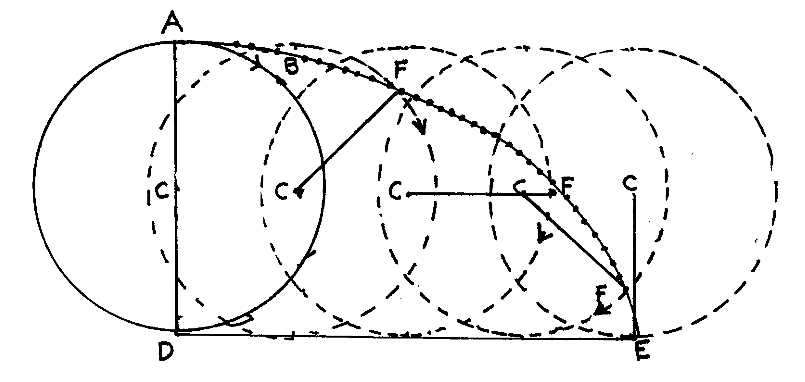
\includegraphics[width=\textwidth]{fig/Figure30}
\caption{}
\label{cycloidfig}
\vspace{-10pt}
\end{center}
\end{figure} There we have a wheel which begins at $ABD$ and has its
center at $C$.  The ground is the horizontal line $DE$.  As the wheel
rolls to the right along the ground the point $A$ will move to new
points $F$ and trace out the {\em cycloid} $AFE$.  We treat the
cycloid in more detail below (page~\pageref{cycloid}), using the
differential calculus.

\subsection*{Note 6}
\label{begtc}
\label{crg6}
Leibniz's argument (and the sketch we give here) is far from a
complete demonstration, but rather a plausible argument to cast doubt
on Descartes' definition of the boundaries of geometry. Leibniz shows
that there are good reasons to believe that the quadratrices for the
circle and hyperbola are, in Descartes' terms, mechanical, and that
Descartes would have to exclude them from geometry.

We will only treat the case of the circle, returning to the case of
the hyperbola later (see below, page~\pageref{begloghyp}).

\vspace{2ex}
\noindent{\bf Theorem:} {\em The quadratrix of a circle is transcendent.}
\vspace{2ex}

\noindent{\bf A sketch of a demonstration:}
  See Figure~\ref{circquad2}.
  \begin{figure}[htp]
\begin{center}
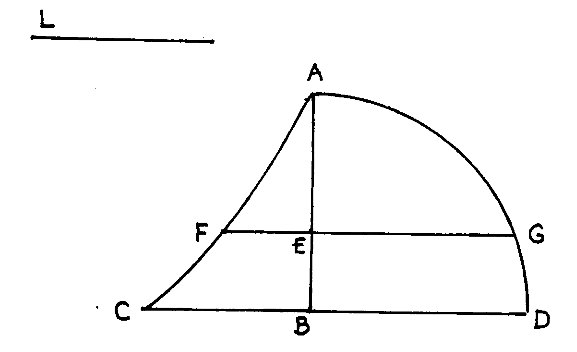
\includegraphics[width=.75\textwidth]{fig/Figure31}
\caption{}
\label{circquad2}
\vspace{-10pt}
\end{center}
\end{figure} 

Let circle $AGD$ be our quadranda, and let its quadratrix be the line
$AFC$, so that $FE$ (or the rectangle $FE$, $L$, where $L$ is a unit)
is always equal to area $AEG$.  Let its abscissas $AE = x$ and its
ordinates $EF = v$.  Leibniz says that $AFC$ is transcendent.  We
argue by {\em reductio ad absurdum}: we (falsely) suppose that $AFC$
is not transcendent, and argue that this leads to an absurdity.
   
For suppose that $AFC$ were not transcendent.  Then it would have a
single algebraic equation of definite degree, such as
$$v^2 = x,$$
or some other algebraic equation where the exponents of $x$ and $v$
were all of definite degrees, that is, all constant whole numbers.

This algebraic equation for the quadratrix could be used to find the
value of $FE$, that is, area $AEG$, for any given value of $AE$.  In
other words, our {\em reductio} assumption is that we can find all the
areas $AEG$ in terms of their sides $AE$ by a {\em single} equation of
{\em definite} degree.

To complete the argument we would then have to demonstrate the following two things:
\begin{enumerate}
\item We first would have to show that, given our {\em reductio}
  assumption, we could find a single algebraic equation of definite
  degree that can be used to divide any angle into any number of equal
  parts.
\item We then would have to show that the problem of dividing an angle
  into an arbitrary number of parts has no definite degree,
  contradicting what we just showed in the first part of the
  demonstration, and thus showing that our assumption that $AFC$ is
  not transcendent must be false.
\end{enumerate}\label{endtc}

We go through these steps in an appendix, pages~\pageref{begapp}--\pageref{endapp}, below.

\subsection*{Note 7}
\label{crg7}

Leibniz claims here, without proof, that finding quadratrices is a
special case of an inverse tangent problem. An inverse tangent problem
is a problem where we are given a property that the tangents of a
curve must have, and we have to find the curve.  Here, instead of
immediately demonstrating that the problem of finding quadratrices is
a special case of the inverse tangent problem, Leibniz first goes on
to show (in this and the following paragraph) how the inverse tangent
problem can be approached by a method that is closely analogous to the
one presented in an earlier paper, ``On finding measurements of
figures," a method which in turn follows Tschirnhaus's method.

\subsection*{Note 8}
\label{crg8}

Here is an example of the solution to an inverse tangent problem,
using the method Leibniz sketches here.  Suppose we are looking for a
curved line $AEB$ (Figure~\ref{invtan})
\begin{figure}[htp]
\begin{center}
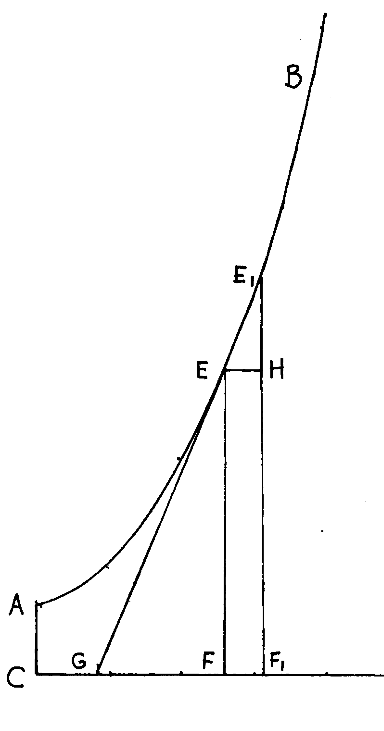
\includegraphics[width=.5\textwidth]{fig/Figure33}
\caption{}
\label{invtan}
\vspace{-10pt}
\end{center}
\end{figure} whose ordinates are $EF$, whose abscissas are $CF$, and
whose tangents $EG$ have the property that
$$\frac{EF}{FG} = CF.$$
If we set $CF=x$ and $EF =y$, and we draw a characteristic triangle
$EE_1H$, then $EH =dx$, and $E_1H=dy$.  Since triangle $EE_1H$ is
similar to triangle $GEF$,
$$\frac{EF}{FG} = \frac{dy}{dx},$$
and therefore, because of our property of tangents,
\begin{equation}
\frac{dy}{dx} = x.
\end{equation}


To find the curve $AEB$ that has equation~1, we first write down a ``general or indefinite equation" for it:
\begin{equation}
\label{geneq}
 0 = a + bx + cy + exy + fx^2 + gy^2 + \mbox{ etc.}
 \end{equation}
 This equation is general or indefinite insofar as its coefficients
 ($a$, $b$, $c$ etc.) are not definite numbers, but general constants,
 each of which could represent any number.  Such an equation can
 represent {\em any} curve that has an algebraic equation, and so, in
 particular, it can represent the curve $AEB$ we are looking for {\em
   if} it has an algebraic equation.

 We then use this general equation to find the tangent of the line, by
 taking its differences and solving for
$\frac{dy}{dx}$, as follows.
\begin{eqnarray*}
0 & = & d(a + bx + cy + exy + fx^2 + gy^2 + \mbox{ etc.}) \\
& = & b\,dx + c\,dy + e\,d(xy) + f\,d(x^2) + g\,d(y^2) +\mbox{ etc.}\\
& = & b\,dx + c\,dy + ex\,dy + ey\,dx + 2fx\,dx + 2gy\,dy + \mbox{ etc.}
\end{eqnarray*}
(We used the multiplication rule and the power rule on the last step.)
Gathering all terms involving $dy$ on the left gives
$$ - c\,dy -ex\,dy - 2gy\,dy + \mbox{ etc.} = b\,dx + ey\,dx + 2fx\,dx +\mbox{ etc.},$$
or
$$dy( - c -ex - 2gy) + \mbox{ etc.} = dx(b + ey + 2fx +\mbox{ etc.}),$$
and therefore (solving for $dy$ and dividing both sides by $dx$),
$$\frac{dy}{dx} = \frac{b + ey + 2fx +\mbox{ etc.}}{- c - ex - 2gy +\mbox{ etc.}}.$$

We then ``compare what [we found] with the given property of the
tangents," by substituting this solution into our equation for
tangents
$$\frac{dy}{dx} = x,$$
as follows:
$$ \frac{b + ey + 2fx +\mbox{ etc.}}{- c - ex - 2gy +\mbox{ etc.}} = x.$$
We then use this last equation to try to find the constants $a$,
$b$, $c$, etc.
In this case, if
$b = e = g = h = \ldots = 0,$ and  $f = -\frac{c}{2},$ then 
$$\frac{b + ey + 2fx +\mbox{ etc.}}{- c - ex - 2gy +\mbox{ etc.}}$$
would simply equal $x$, and therefore the equation 
$$\frac{dy}{dx} =x$$ 
would be satisfied.
Note that there is no restriction on $a$ or $c$.  Substituting these
values back into the general equation (equation~2), gives us a {\em
  definite} equation for $AEB$, that is, it enables us to ``define the
equation of the line sought":
\begin{eqnarray*}
  0 & = & a + 0x + cy + 0xy - \frac{c}{2}x^2 + 0y^2 + \mbox{ etc.}\\
    & = & a + cy - \frac{c}{2}x^2.
\end{eqnarray*}
Simplifying this equation to solve for $y$ gives us
$$cy  =  \frac{c}{2}x^2 - a,\mbox{ and}$$
\begin{equation}
y  =  \frac{1}{2}x^2 - \frac{a}{c}.
\end{equation}
This is the equation for line $AEB$.  ``Some things remain arbitrary," namely, the constant, 
$$\frac{a}{c},$$
because innumerably many lines solve the problem.  In fact, the length
of the line $AC$ in Figure~\ref{invtan} is arbitrary, and corresponds
to
$$-\frac{a}{c}.$$
\setcounter{equation}{0}


\subsection*{Note 9}
\label{crg9}

The problem at the end of ``A New Method" (page~\pageref{begdeb}) is
an inverse tangent problem where ``the comparison does not succeed"
and the line is transcendent.  Recall that in that problem we were
looking for a line $AEB$ (Figure~\ref{transcurv})
\begin{figure}[htp]
\begin{center}
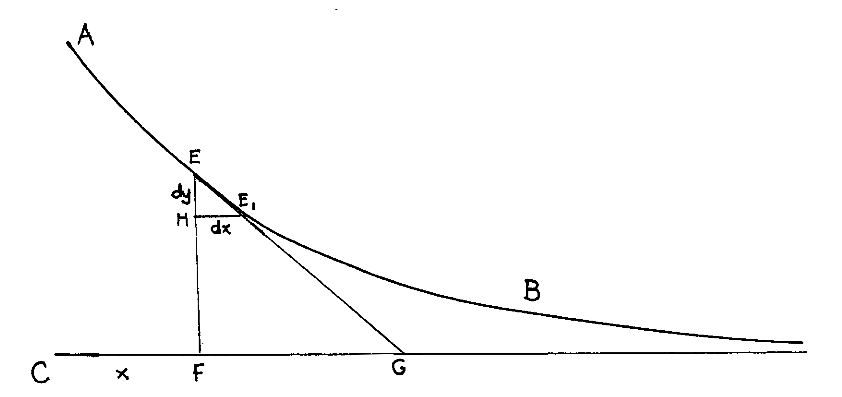
\includegraphics[width=\textwidth]{fig/Figure34}
\caption{}
\label{transcurv}
\vspace{-10pt}
\end{center}
\end{figure} whose tangents had the property that the line $GF$
between the tangents $EG$ and ordinates $EF$ was always equal to a
constant line $k$.  For simplicity, let us suppose $GF= k=1$.  If we
again set $CF =x$ and $EF=y$, then because the characteristic triangle
$EHE_1$ is similar to triangle $GFE$,
$$\frac{EH}{E_1H} = \frac{EF}{GF},$$
and therefore
\begin{equation}
\frac{dy}{dx} = y.
\end{equation}

If, following Leibniz's method, we try to find a solution by using a general or indefinite equation
\begin{equation}
 0 = a + bx + cy + exy + fx^2 + gy^2 + \mbox{ etc.},
 \end{equation}
 we will not succeed.  For, proceeding as in the previous note, we
 will find that there is no way to solve for $a$, $b$, $c$, etc., to
 make the equation
$$\frac{dy}{dx} = y$$
true.
\setcounter{equation}{0}

\subsection*{Note 10}
\label{crg10}

Here Leibniz sketches a way to find more complex transcendents in
terms of simpler ones.  There is thus a kind of order of transcendent
quantities, and the species of a transcendent is its place in this
order: the basic transcendents come from circles and logarithms, and
more complex transcendents can then be defined in terms of these.

To do this, Leibniz chooses a simple given transcendent $v$ and tries
to express the equation for the curve he is looking for in terms of
$x$, $y$, and the transcendent $v$.  For example, the curve might have
the equation
$$y = 3v^2 + 2x.$$
The quantity $y$ is then a new, more complex, transcendent depending on the old transcendent $v$.

The transcendent $v$ might ``depend on the general cutting of a
ratio;" we will see below (page~\pageref{begmprop}) that the logarithm
$$v= \log x$$
is such  a transcendent.  Then the new transcendent $y$ would be equal to 
$$3(\log(x))^2 + 2x.$$



\subsection*{Note 11}
\label{crg11}

To understand what Barrow's theorem is, see Figure~\ref{barrowfig}.
\begin{figure}[ht]
\begin{center}
\includegraphics[width=\textwidth]{fig/Figure41}
\caption{}
\label{barrowfig}
\vspace{-10pt}
\end{center}
\end{figure} 
There we are given an arbitrary curve $AB$ whose axis is $AC$.  The
ordinates $BC$ are equal to $x$, while the abscissas $AC$ are equal to
$y$.  Then for every point $B$ on the curve we extend a {\em
  perpendicular} $BD$ from the curve to the axis.  This perpendicular
creates an {\em interval} $CD = p$ between the ordinate $BC$ and the
perpendicular $BD$ on the axis $AC$.  We then {\em apply} this
interval to the axis by drawing from every point $C$ on the axis a
line $CE$ equal to $CD$ and perpendicular to $AC$. By doing this we
construct a line $AE$ below the axis.  Barrow's theorem asserts that
the {\em sum} of all the intervals ($p= CD = CE$) applied to the
$y$-axis is equal to one half the square on the final ordinate $BC$,
that is, to
  $$ \frac{1}{2}x^2.$$ 
  
  This sum is a sum of infinitely many lines $CE$.  Leibniz does not
  immediately make clear how he understands such an infinite sum.

\subsection*{Note 12}
\label{crg12}

By {\em specious geometry} Leibniz means geometry based on algebra, as
in Descartes' {\em Geometry}.  The term {\em specious} comes from
Vi\`{e}te, who calls the letters for unknown quantities {\em species}
and calls algebra {\em specious arithmetic}.

\subsection*{Note 13}
\label{crg13}
To see where this differential equation comes from, consider
Figure~\ref{barrow1A}, $BD$ is perpendicular to the curve $ABB_1$,
$CD$ is the interval between the ordinate and perpendicular, and
$BGB_1$ is a characteristic triangle.  Let the ordinate $BC = x$ and
the abscissa $AC = y$, so that $B_1G =dx$ and $BG = dy$.  Let
$CD = p$.

Note that triangle $BGB_1$ 
\begin{figure}[htp]
\begin{center}
\includegraphics[width=.75\textwidth]{fig/Figure40}
\caption{}
\label{barrow1A}
\end{center}
\end{figure}
is similar to triangle $BCD$; for angles $BGB_1$ and $BCD$ are both right, and therefore equal; and 
\begin{eqnarray*}
\angle B_1BG + \angle GBD & = & \mbox{the right angle } \angle B_1BD \mbox{, and}\\
\angle CBD + \angle GBD & = &  \mbox{the right angle } \angle CBG,
\end{eqnarray*}
and therefore 
$$\angle B_1BG + \angle GBD = \angle CBD + \angle GBD,$$
and therefore (subtracting  $\angle GBD$ from both sides of this equation)
$$\angle B_1BG=  \angle CBD,$$
so that the triangles $GBB_1$ and $CBD$ share two equal angles, and
are therefore similar.  It follows from the similarity of these two
triangles that
$$B_1G\!:\! BG :: CD \!:\! BC,$$
that is,
$$dx\!:\!dy :: p\!:\!x,$$
and therefore 
$$x\,dx = p\,dy.$$

\subsection*{Note 14}
\label{crg14}

Leibniz denotes the {\em sum} of the infinitely many infinitely small quantities $p\,dy$ by
$$\int\! p\,dy.$$
The symbol $\int$ is an elongated letter $s$.

\subsection*{Note 15}
\label{crg15}

Since 
$$d\left(\frac{1}{2}x^2\right) = x\,dx,$$
it follows that
$$\int\!x\,dx = \int\!d\left(\frac{1}{2}x^2\right).$$
Now, according to Leibniz, sums and differences are reciprocal like
powers and roots.  This means that taking sums undoes what taking
differences does.  Therefore, when we begin with a quantity, take its
differences, and then take the sum of these differences, we get back
the quantity we started with.  In this case
$$ \int\!d\left(\frac{1}{2}x^2\right) = \frac{1}{2}x^2.$$

In Note~19, below (p.~\pageref{crg19}), we demonstrate that sums and differences are reciprocal.

\subsection*{Note 16}
\label{crg16}

To see where Leibniz gets his equation for $a$, let $AB$ be a circle with center $C$ (Figure~\ref{circarc});
\begin{figure}[htp]
\begin{center}
\includegraphics[width=.65\textwidth]{fig/Figure42}
\caption{}
\label{circarc}
\vspace{-10pt}
\end{center}
\end{figure} 
drop a perpendicular $BD$ (the {\em sine} of angle $BCA$ or arc
$a$) from some point $B$ on the circle to the radius $CA$.  Let the
radius $CA=1$, let $AD = x$ (so that $CD = 1-x$) and let arc $AB = a$.
(The line $AD$ in the unit circle is the {\em versed sine}, and the
line $CD$ is the {\em cosine} of angle $BCA$ or arc $a$.\footnote{If
  $AB$ is were not a unit circle, then the ratio $AD/BC$ would be the
  versed sine, $CD/BC$ would be the cosine, and the arc $a$ would
  equal $\displaystyle \frac{\text{arclength }AB}{BC}$, that is, the
  value of arc $AB$ measured in radians.}) Then take a point $B_1$
infinitely close to $B$, and complete the characteristic triangle
$B_1GB$.  Then $B_1G=dx$,\label{b1gpositive} $BG = dy$, and
$B_1B = da$.

Triangle $B_1GB$ is similar to triangle $BDC$; for 
$$\angle B_1GB = \angle BDC,$$
(because they are both right), and
\begin{eqnarray*}
\angle GB_1B + \angle B_1GB + \angle GBB_1 & = & \mbox{two right angles, and}\\
\angle CBD + \angle CBB_1 + \angle GBB_1 & = & \mbox{two right angles.}
\end{eqnarray*}
Therefore 
$$\angle GB_1B + \angle B_1GB + \angle GBB_1 = \angle CBD + \angle CBB_1 + \angle GBB_1, $$
and therefore (canceling $\angle GBB_1$ on both sides)
$$\angle GB_1B + \angle B_1GB  = \angle CBD + \angle CBB_1. $$
But 
$$\angle B_1GB = \angle CBB_1$$
(for they are both right), and therefore
$$\angle GB_1B = \angle CBD.$$
Triangles $B_1GB$ and $BDC$ therefore have two pairs of equal angles, and therefore must be similar.

It follows from the similarity of these triangles that
$$B_1B\!:\! B_1G :: CB\!:\!BD.$$
But
\begin{eqnarray*}
BD&  = & \sqrt{BC^2 - CD^2} \\
& = & \sqrt{1-(1-x)^2}\\
& = & \sqrt{2x -x^2}.\label{sinelength}
\end{eqnarray*}
Therefore (substituting values into the preceding proportion and converting it into an equation)
$$\frac{da}{dx} = \frac{1}{\sqrt{2x-x^2}}.$$ Therefore 
$$da = \frac{dx}{\sqrt{2x-x^2}}.$$
Taking sums of both sides of this equation gives
$$\int\! da =  \int\!\frac{dx}{\sqrt{2x-x^2}}.$$
But since sums and differences are reciprocal,
$$\int\! da = a.$$
Therefore
$$\label{ecircarc} a = \int\!\frac{dx}{\sqrt{2x-x^2}}.$$
This is Leibniz's equation.  It is a simple equation expressing the
transcendent relation between the length of the arc $AB$ of a circle
and its versed sine $AD$.

\subsection*{Note 17}
\label{crg17}

\label{cycloid} Recall that a {\em cycloid} is a curve traced out by a
point on a wheel as the wheel rolls without slipping on level ground.
See Figure~\ref{cyceqfig}.  There we have a wheel which begins at
$ABD$ and has its center at $C$.  The ground is the horizontal line
$DE$.  As the wheel rolls to the right along the ground the point $A$
will move to new points $F$ and trace out the {\em cycloid} $AFE$.

To find an equation for the cycloid, we find the length of the line
$GF$ for a given position of the wheel.  Let $H$ be the point that
ends up on the ground at $D_1$ as the wheel rolls to the right.  Draw
the diameter $KCH$.  Then, when $H$ has moved down to $D_1$, $K$ has
moved up to $A_1$. The point $F$, where $A$ ends up, is then on the
same horizontal line $KGBF$ as the point $K$.  Then, because the wheel
rolls without slipping,
\begin{figure}[htp]
\begin{center}
\includegraphics[width=\textwidth]{fig/Figure43}
\caption{}
\label{cyceqfig}
\vspace{-10pt}
\end{center}
\end{figure} 

$$\mbox{arc }DH = DD_1.$$
But 
$$DD_1 = GG_1,$$
and 
$$\mbox{arc }DH = \mbox{arc }AB,$$
and therefore
\begin{equation}
GG_1 = \mbox{arc }AB.\label{eqcy1}
\end{equation}
Moreover, because $A_1F$ and $AB$ are equal arcs on equal circles, it
follows that the curvilinear triangle $AGB$ is equal and similar to
the curvilinear triangle $A_1G_1F$, and therefore
\begin{equation}
G_1F = GB.\label{eqcy2}
\end{equation}
Putting together equations~\ref{eqcy1} and \ref{eqcy2}, we get an equation for $GF$:
\begin{eqnarray}
GF & = & GG_1 + G_1F\label{eqcy3}\\
& = & \mbox{arc }AB + GB.\label{eqcy4}
\end{eqnarray}

Now, to get Leibniz's equation, we treat $AD$ as the axis of the
cycloid and $FG$ as an ordinate, so that $AG$ is the abscissa, and set
$$AG = x$$ and
$$GF =y.$$
Then, according to equation~\ref{eqcy4},
$$y = \mbox{arc }AB + GB,$$
and in the previous note (page~\pageref{ecircarc}) we showed that 
$$\mbox{arc }AB = \int\!\frac{dx}{\sqrt{2x -x^2}},$$
and (page~\pageref{sinelength})
$$GB = \sqrt{2x-x^2}.$$
Therefore
$$y = FG = \int\!\frac{dx}{\sqrt{2x -x^2}} + \sqrt{2x-x^2}.$$
This is Leibniz's equation. \label{ecycloid}

\subsection*{Note 18}
\label{crg18}

Let $AB$ be a curve, and let $CD$ be its axis. (See Figure~\ref{acurve}.)
\begin{figure}[ht]
\begin{center}
\includegraphics[width=\textwidth]{fig/Figure44}
\caption{}
\label{acurve}
\vspace{-10pt}
\end{center}
\end{figure} 
Let lines $EF$ be the ordinates to the curve.  From every point $E$ on
the curve draw perpendicular lines $EG$ meeting the axis at $G$.  From
$F$, draw perpendicular lines $FL$ below the axis such that
$$FL = EG.$$
Let $HLK$ be the line going through all the points $L$.  Then figure
$CHKD$ is ``the figure made from the perpendiculars to a curve, drawn
ordinatewise to the axis."

Next, rotate the line $AB$ all the way around the axis, so that every
point $E$ moves in a complete circle around the point $F$ on the
axis. (See Figure~\ref{rotate}.)
\begin{figure}[ht]
\begin{center}
\includegraphics[width=\textwidth]{fig/Figure45a}
\caption{}
\label{rotate}
\vspace{-10pt}
\end{center}
\end{figure} As it rotates, the figure $ACDB$ then forms a solid, and
let us call the surface of this solid $AMNB$.  Leibniz saw the
following theorem.

\subsubsection*{Theorem:}

Figure $CHKD$ is proportional to surface $AMNB$.

\hspace{1ex}

\noindent{\bf Demonstration:}

In Figure~\ref{rotate} (p.\pageref{rotate}), consider the ring $ERPP_1R_1E_1$ formed by
rotating the infinitely small line $EE_1$ about the axis.  The area of
the surface $AMNB$ is the sum of all these infinitely small rings.
The circumference of this ring is proportional to its radius $EF$:
$$\mbox{circumference }ERP = 2\pi(EF).$$
(Because $E$ and $E_1$ are infinitely close, the circumference of
circle $ERP$ is equal to the circumference of circle $E_1R_1P_1$.)
The surface area of the ring $ERPP_1R_1E_1$ is equal to its width
($EE_1$) times its circumference ($2\pi (EF)$):
\setcounter{equation}{0}
\begin{equation}
\mbox{area }ERPP_1R_1E_1 = 2\pi \times EE_1 \times EF
\end{equation}


Now, to find $EE_1 \times EF$, turn back to Figure~\ref{acurve}. 
%Figure~\ref{acurve2}. 
Draw
the characteristic triangle $EE_1Q$, the ordinate $E_1F_1$ and the
line $F_1L_1$ equal to the the perpendicular to the curve at $E_1$.
Then %\addtocounter{figure}{-2}
%\begin{figure}[ht]
%\begin{center}
%\includegraphics[width=\textwidth]{fig/Figure44}
%\caption{}
%\label{acurve2}
%\vspace{-10pt}
%\end{center}
%\end{figure}
%\addtocounter{figure}{1}
$$\angle E_1EQ + \angle QEG  = \angle FEG + \angle QEG = \mbox{a right angle.}$$
Therefore
$$\angle E_1EQ = \angle FEG,$$
and the right triangles $E_1EQ$ and $GEF$ are similar.  Therefore
$$\frac{EE_1}{EG} = \frac{EQ}{EF},$$
and therefore
$$EE_1\times EF = EQ \times EG.$$
But $EQ = FF_1,$ and $EG = FL$, and therefore
$$EE_1\times EF = FF_1 \times FL.$$
Now
$FF_1 \times FL$ is equal to the  curvilinear quadrilateral $FF_1L_1L$
(since $FL = F_1L_1$, because $L$ and $L_1$ are infinitely close), and therefore
\begin{equation}
EE_1\times EF = \mbox{quadrilateral }FF_1L_1L.
\end{equation}


Therefore (putting together equations~1 and 2)
\begin{equation}
\mbox{area }ERPP_1R_1E_1 = 2\pi\times \mbox{quadrilateral }FF_1L_1L.
\end{equation}
Equation~3 holds for every point $E$ on the curve $AEB$. We now find
the sums of each side of equation~3 for all points on the curve.  The
sum of the left side of equation~3 is the sum of all the rings
$ERPP_1R_1E_1$ in Figure~\ref{rotate}, that is, the surface $AMNB$.
The sum of the right side is $2\pi$ times the sum of all the
quadrilaterals $FLL_1F_1$ in Figure~\ref{acurve}, that is, $2\pi$
times the whole figure $CHKD$.  Therefore
$$\mbox{surface }AMNB = 2\pi\times \mbox{figure }CHKD,$$
and surface $AMNB$ is proportional to figure $CHKD$.

\noindent  \textsc{q.e.d.}

\subsection*{Note 19}
\label{crg19}

In finding measurements of figures using the calculus, we have
repeatedly used the reciprocity of sums and differences.  In this
note, we demonstrate this reciprocity, which is traditionally called
the {\em fundamental theorem of calculus}.  Before demonstrating the
fundamental theorem, we first need to spell out in greater generality
how sums can be used to find the areas of curvilinear figures.  After
demonstrating the fundamental theorem we will give a number of
examples of how the calculus can be used to determine ``quadratrices
or other lines, algebraic or transcendent" (p.~\pageref{quadothalg}).

\smallskip

This note is divided into five parts:
\vspace{-0.5em}
\begin{enumerate}
\itemsep0em
\item Finding areas of figures with sums.
\item The reciprocity of sums and differences: the fundamental
  theorem.
\item Examples of determining algebraic quadratrices.  Here we show
  how the calculus can be used to find areas under curves in certain
  cases where both the original curve and the equation giving its area
  turn out to be algebraic.
\item A transcendent line: the sine curve.  Here we show the calculus
  can be used to express a transcendent curve that arises from arcs of
  a circle.  After showing what the sine curve looks like and
  demonstrating that it is transcendent, we go on to show how the
  calculus can be used to find sums and differences of expressions
  involving sines and other trigonometric quantities.
\item Another transcendent line: the logarithmic line.  Here we return
  to the logarithmic line, which we saw at the end of ``A New Method".
  Here we show that the logarithmic line is in fact the quadratrix of
  a hyperbola, expand Leibniz's argument from earlier in ``On
  Recondite Geometry" (page~\pageref{logtrans}) that the logarithm is
  transcendent, and go through a number of examples showing how the
  calculus can be used to find sums of expressions involving
  logarithms.
\end{enumerate}

\subsection*{1. Finding areas of figures with sums}

\label{meas} Suppose $AB$ (Figure~\ref{areasum})
\begin{figure}[htp]
\begin{center}
\includegraphics[width=.75\textwidth]{fig/Figure35}
\caption{}
\label{areasum}
\vspace{-10pt}
\end{center}
\end{figure} is a curved line with axis $AC$ and ordinates $EF$, and
we want to find the area $AEBC$.  Let the ordinates $EF =v$ and the
abscissas $AF=x$.  Draw an arbitrary number of ordinates $E_1F_1=v_1$,
$E_2F_2=v_2$, etc.  Let $BC=v_4$, and suppose $AF_1=dx_1$,
$F_1F_2 =dx_2$, $F_2F_3= dx_3$, and $F_3C = dx_4$.  The area $ABC$ is
of course equal to the sum of the four areas $AE_1F_1$,
$E_1E_2F_2F_1$, $E_2E_3F_3F_2$, and $E_3BCF_3$.  Each of these four
areas is still curvilinear, and it is therefore difficult to come up
with a numerical value for each. But if we draw the rectangles
$AGE_1F_1$, $F_1G_1E_2F_2$, $F_2G_2E_3F_3$, and $F_3G_3BC$, making a
polygon $AGE_1G_1E_2G_2E_3G_3BC$, which we will call $P$, we can
compute the area of this polygon as a sum of these four rectangles
\setlength{\jot}{1.5ex}
\begin{eqnarray*}
  P & =  & AGE_1F_1 + F_1G_1E_2F_2 + F_2G_2E_3F_3 + F_3G_3BC\\
    & = & (AF_1 \times F_1E_1) + (F_1F_2\times F_2E_2) + (F_2F_3 \times F_3E_3) + (F_3C \times CB)\\
    & = & v_1\,dx_1 + v_2\,dx_2 + v_3\,dx_3 + v_4\,dx_4.
\end{eqnarray*}
\setlength{\jot}{\oldjot}
\hspace{-.35em}Thus the area of a polygon, unlike a curvilinear area,
can be computed by finding a finite sum.

Now polygon $P$ is greater than the curvilinear area $ABC$ we are
interested in.  But if we had taken more points $E_1$, $E_2$, etc., we
would have found a polygon that was closer to this area, and we could
make the difference between the area of our polygon and our
curvilinear area less than any given difference.  Therefore if we take
a polygon $P$ with infinitely many sides, we may treat it as exactly
equal to the curvilinear area $ABC$.  The area of the whole infinite
polygon $AGE_1G_1\ldots BC$ (that is, the curvilinear area $ABDC$) is
equal to
$$v_1\,dx_1 + v_2\,dx_2 + v_3\,dx_3 + \ldots$$
We can thus compute the curvilinear area $ABC$ by finding an {\em
  infinite} sum of {\em infinitely small} quantities.  Leibniz denotes
this sum by
$$\int\!v\,dx;$$
the symbol $\int$ indicates that a sum is being taken, while $v\,dx$
indicates what is being summed: the products of the ordinates $v$
times the infinitely small differences of the abscissas $dx$.  One
could read the whole symbol $\int\!v\,dx$ as ``the sum of the
ordinates applied to the axis."

(Shortly after Leibniz introduced this new symbol for infinite sums,
other mathematicians began calling them {\em integrals}, and that soon
became the standard name.  We usually read
$$\int\!v\,dx$$
as ``the integral of $v\,dx$."  Summing is called {\em integrating}.)

%\label{quadsum} Let $AGD$ (Figure~\ref{quadsum})
%\begin{figure}[htp]
%\begin{center}
%\includegraphics[width=.75\textwidth]{fig/Figure31}
%\caption{}
%\label{quadsum}
%\vspace{-10pt}
%\end{center}
%\end{figure}  be any line, let $AB$ be its axis, let its ordinates $EG =v$ and the abscissas $AE =x$, then the area $AEG$ is 
%$$\int \! v\,dx.$$
%Now if $AFC$ is the quadratrix of $AGD$, and we let $L$ be a unit, then 
%$$FE = FE \times L  = \mbox{area }AEG.$$
%Therefore
%$$FE = \int\! v\,dx,$$
%that is, {\em the ordinate of a quadratrix is equal to the sum of the ordinates of the quadranda times the differences of its abscissas.}  Finding sums thus lets us find quadratrices.

Note that a sum has to begin and end at some definite points: here we
have found the sum beginning from $A$ and ending at $C$.  We could
have begun or ended the sum at any definite ordinates.  In general, it
will be clear from the problem we are considering where the sum should
begin. Most often, we simply begin the sum at a point where the
quantity whose differences appear in the sum is equal to zero; here we
are considering
$$\int\! v\,dx,$$
a sum involving $dx$, and we begin the sum where $x=0$, that is, at
the point $A$.  We usually let the endpoint of the sum be an
undetermined variable.  When we want to make explicit where the sum
begins and ends, we attach quantities to the summing sign, as follows:
$$\int^3_0\!v\,dx,$$
denotes the sum beginning at $x=0$ and ending at $x=3$ (see Figure~\ref{sum03}),
\begin{figure}[htp]
\begin{center}
\includegraphics[width=\textwidth]{fig/Figure36B}
\caption{}
\label{sum03}
\vspace{-10pt}
\end{center}
\end{figure} 
and, in general,
$$\int^b_a\!v\,dx$$
denotes the sum beginning at $x=a$ and ending at $x=b$ (see Figure~\ref{sumab}).
\begin{figure}[htp]
\begin{center}
\includegraphics[width=\textwidth]{fig/Figure36C}
\caption{}
\label{sumab}
\vspace{-10pt}
\end{center}
\end{figure} 

\subsection*{2. Sums and differences as inverses}

To show that sums and differences are reciprocal, we need to demonstrate two theorems:
\begin{enumerate}
\itemsep0em
\item that if we find a difference and then find its sum, we get back
  to where we started; and
\item that if we find a sum and then find its difference, we get back
  to where we started.
\end{enumerate}
These two theorems show that finding sums is a sort of mirror image of
finding differences, just as finding square roots is a mirror image of
finding squares.  What finding differences does, finding sums undoes,
and vice versa.  Everything we know about differences is therefore
reflected in sums, and, therefore also in finding measurements of
figures.  These theorems are thus the foundation of the application of
the differential calculus to problems of finding measurements of
figures, and we therefore name them the {\em first} and {\em second
  fundamental theorems}.

\subsubsection*{First Fundamental Theorem}
\label{fund1} For any variable quantity
$$\int\!dv = v.$$

\noindent {\bf Demonstration:} 
Let the line $AB$ represent the quantity $v$. (See Figure~\ref{ffundfig}.)
\begin{figure}[htp]
\begin{center}
\includegraphics[width=.75\textwidth]{fig/Figure37}
\caption{}
\label{ffundfig}
\vspace{-10pt}
\end{center}
\end{figure} Take infinitely many infinitely close points $C_1$,
$C_2$, etc.\ on the line, so that $AC_1 = v_1$, $AC_2 =v_2$,
$AC_3 =v_3$, etc.  Therefore $AC_1 =dv_1$, $C_1C_2 = dv_2$, etc. Then
\begin{eqnarray*}
  \int\!dv & = & dv_1 + dv_2 + \ldots\\
           & = & AC_1 + C_1C_2 + C_2C_3 +\ldots \\
           & = & AB\\
           & = & v. \mbox{\hspace{10ex}  \textsc{q.e.d.}}
\end{eqnarray*}

Note that it is important here that we begin the sum at the point where $v=0$.


\subsubsection*{Second Fundamental Theorem}
\label{fund2}  Given an infinitely small variable quantity $y\,dx$,
$$d\int\!y\,dx = y\,dx.$$

\noindent {\bf Demonstration:}
Let $AB$ be a curved line with axis $CD$, ordinates $EF=y$ and
abscissas $CF = x$.  (See Figure~\ref{sfundfig}.)
\begin{figure}[htp]
  \begin{center}
    \includegraphics[width=\textwidth]{fig/Figure38}
    \caption{}
    \label{sfundfig}
    \vspace{-10pt}
  \end{center}
\end{figure}

Let us denote the variable area $ACFE$ by $v$.  Then 
$$v = \int\!y\,dx.$$

Let $E_1$ be a point infinitely close to $E$ on the curve, and drop an
ordinate $E_1F_1$ to the axis.  Let $CF_1 = x_1$ and $ACF_1E_1 = v_1$.
Then
$$dx = x_1 - x = FF_1,$$
and
$$dv = v_1 - v = ACF_1E_1 - ACFE = EFF_1E_1.$$
But since $E$ and $E_1$ are infinitely close, we may take
$EF = E_1F_1$ and treat $EFF_1E_1$ as a rectangle.  Its area is
therefore equal to $EF$ times $FF_1$, that is, to $y\,dx$.  Therefore
$$dv = y\,dx,$$
that is,
$$d\int\!y\,dx = y\,dx.$$
\textsc{q.e.d.}

The second fundamental theorem says that any infinitely small variable
quantity $y\,dx$, is equal to the difference of its sums.
%Note that all infinitely small variable quantities can be expressed in the form $y\,dx$, where $y$ is some variable quantity.  For if $z$ is any infinitely small variable quantity, then we can set 
%$$y = \frac{z}{dx},$$
%so that 
%$$z = y\,dx.$$
%Note also that when we write our infinitely small quantity as $y\,dx$ we are not assuming that it is itself a difference, but only that it is a product of a variable quantity and a difference.

%In reading ``A New Method," we interpreted differences geometrically using tangents of lines.  Here we are interpreting sums geometrically using areas of figures.  The second fundamental theorem thus shows that finding tangents of lines and finding areas of figures are inverse problems.  Let $AGD$ (see Figure~\ref{fundquad})
%\begin{figure}[htp]
%\begin{center}
%\includegraphics[width=.75\textwidth]{fig/Figure39}
%\caption{}
%\label{fundquad}
%\vspace{-10pt}
%\end{center}
%\end{figure}  be a given line, let its abscissas $AE=x$, and let its ordinates $EG=y$.  Let $AFC$ be the quadratrix of $AGD$, and let its ordinates $EF =v$.  Therefore,  for any point $G$,
%\begin{eqnarray*}
%FE & = & \mbox{area }AEG,\mbox{ that is,}\\
%v & = & \int\! y\, dx.
%\end{eqnarray*}
%Let $FK$ be tangent to $AFC$ at $F$.  Then, as we saw in ``A New Method," 
%$$\frac{FE}{EK} = \frac{dv}{dx}.$$
%According to the second fundamental theorem,
%$$dv = y\,dx,$$
%an therefore
%\setlength{\jot}{2ex}
%\begin{eqnarray*}
%\frac{FE}{EK} & = & \frac{y\,dx}{dx}\\
%&  = & y\\
%& = & EG.
%\end{eqnarray*}
%\setlength{\jot}{\oldjot}
%In other words, {\em the slope of the tangent to the quadratrix is equal to the ordinate of the quadranda.}  The rate of change of the ordinate of the quadratrix is thus proportional to the size of the ordinate of the quadranda.
%

%%%%%%%%%%%%%%%%%%%%%%%%%%%%%%%%%%%%%%%%%%%%%%%%%%%%%%%%%%%%%%%%%%%%%%%%%%%%%%%%%%%%%%%%%%%%%%%%%%%%%
%%%%%          The following, sections 3--5 of note 19, is replaced by the            %%%%%%%%%%%%%%%
%%%%%          corresponding sections of the 2014 manual. June  5, 2016               %%%%%%%%%%%%%%%
%%%%% %%%%%%%%%%%%%%%%%%%%%%%%%%%%%%%%%%%%%%%%%%%%%%%%%%%%%%%%%%%%%%%%%%%%%%%%%%%%%%%%%%%%%%%%%%%%%%%%
%%%%% \subsection*{3. Examples of determining algebraic quadratrices}

%%%%% In all the following examples we are given a curved line $ADB$ (Figure~\ref{algquad})
%%%%% \begin{figure}[htp]
%%%%% \begin{center}
%%%%% \includegraphics[width=.9\textwidth]{fig/Figure46}
%%%%% \caption{}
%%%%% \label{algquad}
%%%%% \vspace{-10pt}
%%%%% \end{center}
%%%%% \end{figure} whose axis is $AEC$ and whose ordinates are $DE$.  Let
%%%%% $AE = x$ and $DE = y$.  Let the curve $AFG$ be the quadratrix of the
%%%%% curve $ADB$ (the quadranda), that is, let the ordinate $EF$ of $AFG$
%%%%% always be equal to the curvilinear area $ADE$.  Let $v = EF$, so that
%%%%% $v$ is always equal to the area $ADE$.  Then
%%%%% $$v = \int\!y\,dx.$$
%%%%% To find an equation for the quadratrix $AFG$ we have to find an
%%%%% equation relating $v$ to $x$, that is we have to find the area
%%%%% $\int\! y\,dx$ in terms of $x$.

%%%%% To find $v$, we use the second fundamental theorem.  If
%%%%% $$v = \int\! y\,dx,$$
%%%%% then, according to the second fundamental theorem,
%%%%% $$dv = y\,dx.$$
%%%%% Therefore, given $y$, we need to find a quantity $v$ such that $dv/dx$
%%%%% is equal to $y$; that is, we need to find a quantity $v$ whose
%%%%% differences are equal to $y\,dx$.  Thus finding sums is in general
%%%%% much more difficult than finding differences.  To find differences we
%%%%% simply have to follow mechanically the rules Leibniz has given us in
%%%%% ``A New Method."  But there is no complete set of rules for going
%%%%% backwards and, given a quantity $y$, to find a quantity $v$ whose
%%%%% differences are equal to $y\,dx$.  In an earlier paper Leibniz writes
%%%%% that
%%%%% \begin{quote}
%%%%%   But this is the labor, this is the task: given a Quadranda, to find
%%%%%   some Quadratrix for it; this is especially difficult because
%%%%%   sometimes it is impossible to find a quadratrix (at least one that
%%%%%   can be expressed algebraically).\footnote{``On Finding Measurements
%%%%%     of Figures," published in the {\em Acts} in May of 1684.  It is on
%%%%%     pages~123--6 in Volume~V of Gerhardt's edition.}
%%%%% \end{quote}
%%%%% He is alluding here to Book VI of Virgil's {\em Aeneid} where the Cumaean Sybil says to Aeneas
%%%%% \begin{verse}
%%%%%   Born of the blood \\
%%%%%   of gods and son of Troy's Anchises, easy---\\
%%%%%   the way that leads to into Avernus: day \\
%%%%%   and night the door of darkest Dis is open.\\
%%%%%   But to recall your steps, to rise again \\
%%%%%   into the upper air: that is the labor;\\
%%%%%   that is the task.\footnote{Lines 174--180 of Allen Mandelbaum's
%%%%%     translation.  Lines 125--129 of R.\ A.\ B.\ Mynors's Latin text.}
%%%%% \end{verse}

%%%%% \label{alg_int} While there is no general method for finding sums,
%%%%% there is one difficulty that always arises and may be treated
%%%%% methodically.  Let
%%%%% $$v = \int\! y\,dx,$$
%%%%% so that, by the second fundamental theorem, 
%%%%% $$dv = y\,dx.$$
%%%%% Suppose we have managed to find an expression for a quantity $w$ such
%%%%% that $dw = y\,dx$.  Then $dv = dw$, and therefore $d(v-w) =0$, and
%%%%% $v-w$ must be constant.  Let $v-w = C$.  Then $v = w + C$.  To
%%%%% complete the solution of the problem, we need to find $C$.  We can do
%%%%% so by setting $w+ C =0$ at the point where the sum begins.

%%%%% Here are some examples.

%%%%% \begin{enumerate}
%%%%% \item Let $y = x^2$, so that
%%%%%   $v = \mbox{area }ADE = \int \!y\,dx = \int\! x^2\,dx.$ According to
%%%%%   the second fundamental theorem, $dv = x^2\,dx$.  So let us find an
%%%%%   expression $w$ such that $dw = x^2\,dx$, then set $v= w+C$ for some
%%%%%   constant $C$, and, finally, solve for $C$.

%%%%% First we need  to find $w$ such that $dw = x^2\,dx$. We know from the rules of the calculus that 
%%%%% \setlength{\jot}{1.5ex}
%%%%% \begin{eqnarray*}
%%%%% d\left(\frac{x^3}{3}\right) & = & \frac{d(x^3)}{3}\\
%%%%% & = &\frac{3x^2\,dx}{3}\\
%%%%% & = & x^2\,dx\\
%%%%% & = & y\,dx.
%%%%% \end{eqnarray*}
%%%%% Therefore let us set $\displaystyle w=\frac{x^3}{3}$, so that $\displaystyle v = w+C =\frac{x^3}{3} + C.$

%%%%% Finally, to find $C$, we set $w+C =0$ at the point where the sum
%%%%% begins.  Here the sum begins where $x=AE =0$.  Therefore, when $x=0$,
%%%%% $$\frac{x^3}{3} + C = 0,$$
%%%%% that is, $0+ C=C =0$. 
%%%%% Therefore
%%%%% $$v =  w = \frac{x^3}{3}.$$
%%%%% We conclude that
%%%%% $$\mbox{area }ADE  =  v = \frac{x^3}{3}.$$
%%%%% Therefore the equation of the quadratrix $AFG$ is in this case\label{int1}
%%%%% $$v= \frac{x^3}{3}.$$

%%%%% \item Let $y = x^3$, so that $v= \int\!y\,dx = \int\!x^3\,dx$.
%%%%%   According to the second fundamental theorem, $dv = x^3\,dx$.  So let
%%%%%   us find an expression $w$ such that $dw = x^3\,dx$, then set
%%%%%   $v= w+C$ for some constant $C$, and, finally solve for $C$.

%%%%%  First we need to find some $w$ such that $dw = x^3\,dx$.  We know from the rules of the calculus that 
%%%%% \setlength{\jot}{1.5ex}
%%%%% \begin{eqnarray*}
%%%%% d\left(\frac{x^4}{4}\right) & = & \frac{d(x^4)}{4}\\
%%%%% & = &\frac{4x^3\,dx}{4}\\
%%%%% & = & x^3\,dx\\
%%%%% & = & y\,dx.
%%%%% \end{eqnarray*}
%%%%% Therefore let us set $\displaystyle w=\frac{x^4}{4}$, so that $\displaystyle v = w+C = \frac{x^4}{4} + C.$

%%%%% Finally, to find $C$, we set $w+C =0$ at the point where the sum
%%%%% begins.  Here the sum begins where $x=AE =0$.  Therefore, when $x=0$,
%%%%% $$\frac{x^4}{4} + C = 0,$$
%%%%% that is, $0+ C=C =0$. 
%%%%% Therefore
%%%%% $$v =  w = \frac{x^4}{4}.$$
%%%%% We conclude that
%%%%% $$\mbox{area }ADE  =  v = \frac{x^4}{4}.$$
%%%%% Therefore the equation of the quadratrix $AFG$ is in this case
%%%%% $$v= \frac{x^4}{4}.$$

%%%%% \item \label{intxn}Let $y=x^n$, where $n$ is any nonnegative number.
%%%%%   We proceed just as in the previous two examples, finding a quantity
%%%%%   $w$ such that $y\,dx = dw$, setting $v =w+C$, an solving for $C$ by
%%%%%   setting $w+C =0$ when $x=0$.

%%%%% We know from the rules of calculus that 
%%%%% \setlength{\jot}{1.5ex}
%%%%% \begin{eqnarray*}
%%%%% d\left(\frac{x^{(n+1)}}{n+1}\right) & = & \frac{d(x^{(n+1)})}{n+1}\\
%%%%% & = &\frac{(n+1)x^n\,dx}{n+1}\\
%%%%% & = & x^n\,dx\\
%%%%% & = & y\,dx.
%%%%% \end{eqnarray*}
%%%%% We therefore set 
%%%%% $$w = \frac{x^{(n+a)}}{n+1}.$$
%%%%% so that 
%%%%% $$v = \frac{x^{(n+1)}}{n+1} + C.$$

%%%%% Finally, to find $C$, we set $w+C =0$ at the point where the sum
%%%%% begins.  Here again the sum begins where $x=AE =0$.  Therefore, when
%%%%% $x=0$,
%%%%% $$\frac{x^{(n+1)}}{n+1} + C = 0,$$
%%%%% that is, $0+ C=C =0$. 
%%%%% Therefore
%%%%% $$v =  w =  \frac{x^{(n+1)}}{n+1}.$$
%%%%% We conclude that
%%%%% $$\mbox{area }ADE  =  v =  \frac{x^{(n+1)}}{n+1}.$$
%%%%% Therefore the equation of the quadratrix $AFG$ is in this case
%%%%% $$v= \frac{x^{(n+1)}}{n+1}.$$

%%%%% \item Let $y = x^3 + x^2.$  Then, if we set 
%%%%% $$w= \frac{x^4}{4} + \frac{x^3}{3},$$
%%%%% according to the rules of calculus,
%%%%% $$dw = x^3\,dx + x^2\,dx = y\,dx.$$
%%%%% Therefore $$w + C = \int\!y\,dx.$$

%%%%% The quantity $w+C$ must be equal to zero when $x=0$, and therefore
%%%%% $$\frac{0^4}{4} + \frac{0^3}{3} + C = C = 0.$$
%%%%% Therefore
%%%%% $$\int\!y\,dx = w + 0 = \frac{x^4}{4} + \frac{x^3}{3}.$$

%%%%% Note that here it turns out that 
%%%%% $$\int\!(x^3+x^2)\,dx = \int\!x^3\,dx + \int\!x^2\,dx.$$
%%%%% This is generally true: for any variable quantities $t$ and $u$,
%%%%% $$\int\!(t+u) = \int\!t + \int\!u.$$
%%%%% For if $t = dv$ and $u = dw$, then 
%%%%% $$d(v+w) = dv + dw = t + u,$$
%%%%% and if we begin the sums when $v=0$ and $w=0$ then we will also begin
%%%%% the sums where $v+w = 0$, and according to the first fundamental
%%%%% theorem, \setlength{\jot}{1.5ex}
%%%%% \begin{eqnarray*}
%%%%% \int\!(t+u) & = & \int\!d(v+w)\\
%%%%% & = & (v+w)\\
%%%%% & = & \int\!dv + \int\!dw\\
%%%%% & = & \int\!t + \int\!u.
%%%%% \end{eqnarray*}
%%%%% \setlength{\jot}{\oldjot}
%%%%% \hspace{-.4em}We might call this the {\em addition rule for sums}.  We
%%%%% could likewise show that for any constant $a$ and any variable $t$
%%%%% $$\int\!at = a\int\!t.$$
%%%%% This could be called {\em constant multiple rule for sums}.

%%%%% We can use these rules, and the rule from the third example, to find
%%%%% sums for many algebraic expressions, as in the following example.

%%%%% \item
%%%%% Let $y = 3x^5 - 8x^2 + 4.$
%%%%% Then
%%%%% \setlength{\jot}{1.5ex}
%%%%% \begin{eqnarray*}
%%%%% \int\!y\,dx & = & 3\int\!x^5\,dx- 8\int\!x^2\,dx + 4\int\!x^0\,dx\\
%%%%% & = & 3\frac{x^6}{6} - 8\frac{x^3}{3} + 4\frac{x^1}{1}\\
%%%%% & = & \frac{x^6}{2} - \frac{8x^3}{3} + 4x.
%%%%% \end{eqnarray*}
%%%%% \setlength{\jot}{\oldjot}

%%%%% \item
%%%%% Let 
%%%%% $$y = 2\sqrt{x} - 8x^{\frac{5}{3}}.$$
%%%%% Then
%%%%% \setlength{\jot}{2ex}
%%%%% \begin{eqnarray*}
%%%%%   \int\!y\,dx & = & 2\int\!x^{\frac{1}{2}}\,dx - 8\int\!x^{\frac{5}{3}}\,dx\\
%%%%%               & = & 2\left(\frac{x^{\frac{3}{2}}}{\frac{3}{2}}\right) - 8\left(\frac{x^{\frac{8}{3}}}{\frac{8}{3}}\right)\\
%%%%%               & = & \frac{4x^{\frac{3}{2}}}{3} - 3x^{\frac{8}{3}}.
%%%%% \end{eqnarray*}
%%%%% \setlength{\jot}{\oldjot}
%%%%% \end{enumerate}

%%%%% \label{defint}
%%%%% Now suppose that we are interested not in the area $ADE$, but in the
%%%%% area $DEE_1D_1$ (see Figure~\ref{sumab2})
%%%%% \begin{figure}[htp]
%%%%% \begin{center}
%%%%% \includegraphics[width=\textwidth]{fig/Figure47}
%%%%% \caption{}
%%%%% \label{sumab2}
%%%%% \vspace{-10pt}
%%%%% \end{center}
%%%%% \end{figure} between two definite ordinates, $DE$ and $DE_1$.  Let
%%%%% $AE =a$ and $AE_1 =b$, where $a$ and $b$ are constants.  This area is
%%%%% equal to the sum of $y\,dx$ between $x=a$ and $x=b$, which we denote
%%%%% by
%%%%% $$\int_a^b\!y\,dx.$$
%%%%% This sum is called a {\em definite integral}, because, unlike the sums
%%%%% in the previous examples, it represents a single constant area, and
%%%%% not a variable area.  To find the area $DEE_1D_1$, we take the
%%%%% difference of the area $AD_1E_1$ (this area is equal to the value of
%%%%% $v$ when we set $x=b$, which we will call $v_b$) and the area $ADE$
%%%%% (this area is equal to the value of $v$ when we set $x=a$, which we
%%%%% will call $v_a$):
%%%%% \begin{eqnarray*}
%%%%%   \mbox{area }DEE_1D_1 & = & \mbox{area }AD_1E_1 - \mbox{area }ADE\\
%%%%%                        & = & v_b - v_a.
%%%%% \end{eqnarray*}

%%%%% In finding definite integrals, we proceed in the same way as before,
%%%%% first finding a quantity $w$ such that $dw = y\,dx =dv$.  It follows
%%%%% that $v = w+C$ for some $C$.  Therefore the definite integral
%%%%% \begin{align*}
%%%%%   \int_a^b\!y\,dx = & v_b -v_a \\
%%%%%   = & w_b+C - w_a+C\\
%%%%%   = & w_b - w_a.
%%%%% \end{align*}
%%%%% Thus we can skip here the step of finding $C$: we simply find any
%%%%% quantity $w$ whose differences are equal to the quantity $y\,dx$ we
%%%%% want to integrate, and take the difference of its value at the last
%%%%% point of the sum and its value at the first.  Of course, if it is
%%%%% convenient, we can always set $w=v$.  It usually will be convenient to
%%%%% do so when $y$ is a simple algebraic quantity, but when $y$ is
%%%%% transcendent this is generally not the case, as we will see below.

%%%%% Here are two simple examples of definite integrals where $y$ is an algebraic quantity.

%%%%% \begin{enumerate}
%%%%% \setcounter{enumi}{6}

%%%%% \item Let $y = x^2$. Then, as we saw above (page~\pageref{int1}), if
%%%%% $$w= \frac{x^3}{3},$$
%%%%% then $dw = x^2\,dx.$  (Here $w = v$, but we could use $w = v +C$ for any $C$.)
%%%%% Now if $a = AE = 2$ and $b= AE_1 = 4,$ then 
%%%%% \setlength{\jot}{2ex}
%%%%% \begin{eqnarray*}
%%%%% \mbox{area }DEE_1D_1 & = & \int_2^4\! y\,dx\\
%%%%% & = & w_4 -w_2\\
%%%%% & = & \frac{4^3}{3} - \frac{2^3}{3}\\
%%%%% & = & \frac{64}{3} - \frac{8}{3}\\
%%%%% & = & \frac{56}{3}.
%%%%% \end{eqnarray*}


%%%%% \item Let $y = 3x^2 + 7x$.  Then
%%%%% \begin{eqnarray*}
%%%%% v & = & \int\!y\,dx\\
%%%%% & = & 3\int\! x^2\,dx + 7\int\!x\,dx\\
%%%%% & = & 3\frac{x^3}{3} + 7\frac{x^2}{2}\\
%%%%% & = & x^3 + \frac{7x^2}{2}.
%%%%% \end{eqnarray*}
%%%%% Here we could take $w= v + C$ for any value of $C$, but it is simplest to set $C=0$ and use $v$ by  itself.
%%%%% Now if $a = AE = 1$ and $b = AE_1 = 5$, then
%%%%% \begin{eqnarray*}
%%%%% \mbox{area }DEE_1D_1 & = & \int_1^5\! y\,dx\\
%%%%% & = & v_5 -v_1\\
%%%%% & = & \left(5^3 + \frac{7(5^2)}{2}\right) - \left(1^3 + \frac{7(1^2)}{2}\right)\\
%%%%% & = & \left(125 + \frac{175}{2}\right) - \left(1 + \frac{7}{2}\right)\\
%%%%% & = & \frac{425}{2} - \frac{9}{2}\\
%%%%% & = & \frac{416}{2}\\
%%%%% & = & 213.
%%%%% \end{eqnarray*}

%%%%% \setlength{\jot}{\oldjot}


%%%%% \end{enumerate}

%%%%% \subsubsection*{Some problems on sums of algebraic quantities}

%%%%% \label{pset5} Find the following sums.

%%%%% \begin{enumerate}

%%%%% \item $$\int\!(2x^3 - x + 4)\,dx.$$

%%%%% \item $$\int\!(3x^5 -2x^2 + 1) \,dx.$$

%%%%% \item $$\int\!(\sqrt{x} + (\sqrt{x})^3)\,dx.$$

%%%%% \item $$\int\!(x^3 + \sqrt[3]{x})\,dx.$$

%%%%% \item $$\int_1^3 \!x^3\,dx.$$

%%%%% \item $$\int_{-1}^1 x^4\,dx.$$

%%%%% \item $$\int_{1}^2\!(5x^4 - 2x)\,dx.$$

%%%%% \item $$\int_{-1}^2\!(2x^2 +1)\,dx.$$

%%%%% \end{enumerate}

%%%%% \subsection*{4. A transcendent line: the sine curve}

%%%%% \label{begsin} In the above examples we always begin with an algebraic
%%%%% curve and end with an algebraic quadratrix: the equation for the
%%%%% original curve $ADB$ (that is, the equation relating $y$ and $x$) and
%%%%% the final equation for the quadratrix $AFG$ (that is, the equation
%%%%% relating $v$ and $x$) are both ordinary algebraic equations (see
%%%%% Figure~\ref{algquad}, page~\pageref{algquad}). Let us now consider
%%%%% some transcendent equations, beginning with Leibniz's equation for the
%%%%% length of an arc of a circle (on page~\pageref{lcircarc} of his
%%%%% text--- see Figure~\ref{circarc2} here):
%%%%% $$a =  \int \!\frac{dx}{\sqrt{2x-x^2}}.$$
%%%%% \begin{figure}[htp]
%%%%%   \begin{center}
%%%%%     \includegraphics[width=.65\textwidth]{fig/Figure42}
%%%%%     \caption{}
%%%%%     \label{circarc2}
%%%%%     \vspace{-10pt}
%%%%%   \end{center}
%%%%% \end{figure} 

%%%%% Leibniz has a given an equation relating the {\em versed sine}, $x$
%%%%% ($DA$ in Figure~\ref{circarc2}), to the arc $a$ ($AB$).  But it will
%%%%% be simpler for us to use an equation relating the {\em sine}, $y$
%%%%% ($BD$), to $a$.  To get such an equation we again use the
%%%%% characteristic triangle $B_1GB$ (see the twelfth note, above,
%%%%% page~\pageref{crg12}).  Because triangle $B_1GB$ is similar to
%%%%% triangle $BDC$,
%%%%% $$B_1B \!:\! BG :: CB \!:\!CD.$$
%%%%% Now $B_1B = da$, $BG = dy$, $CB = 1$, and 
%%%%% \setlength{\jot}{1.5ex}
%%%%% \begin{eqnarray*}
%%%%% CD & = & \sqrt{CB^2 - DB^2} \mbox{\hspace{2ex} (by the Pythagorean theorem)}\\
%%%%% & = & \sqrt{1 - y^2}.
%%%%% \end{eqnarray*}
%%%%% \setlength{\jot}{\oldjot}
%%%%% Therefore (substituting into this proportion and converting it to an equation)
%%%%% $$\frac{da}{dy} = \frac{1}{\sqrt{1-y^2}}.$$
%%%%% Therefore
%%%%% $$da = \frac{dy}{\sqrt{1-y^2}},$$
%%%%% and (taking sums of both sides of the equation and using the first fundamental theorem)
%%%%% $$a = \int\!\frac{dy}{\sqrt{1-y^2}}.$$
%%%%% (Note that this becomes the same equation Leibniz gives on
%%%%% page~\pageref{rgcircarc} of ``On Recondite Geometry," if we substitute
%%%%% $x$ for $y$.)

%%%%% Now, in Figure~\ref{circarc2}, $y$ is a variable straight line while
%%%%% $a$ is a variable curved line.  But we usually (following Descartes)
%%%%% represent an equation by taking both variables to correspond to {\em
%%%%%   straight} lines.  Figure~\ref{sinecurve}
%%%%% \begin{figure}[htp]
%%%%% \begin{center}
%%%%% \includegraphics[width=\textwidth]{fig/Figure48}
%%%%% \caption{}
%%%%% \label{sinecurve}
%%%%% \vspace{-10pt}
%%%%% \end{center}
%%%%% \end{figure} 
%%%%% does this, showing the curve for the same equation when we take both
%%%%% $y$ and $a$ to be variable straight lines.  There we draw an $a$-axis
%%%%% $FG$ and a $y$-axis $FK$.  For any point $M$ on the axis $FG$, if
%%%%% $FM= a$ ($=\mbox{arc }AB$ in Figure~\ref{circarc2}), then we set
%%%%% $ML=y$ ($=BD$ in Figure~\ref{circarc2}). To see why the curve in
%%%%% Figure~\ref{sinecurve} has the shape it does, imagine what happens as
%%%%% $a$ increases uniformly.  In Figure~\ref{circarc2}, as $a$ increases
%%%%% the point $B$ moves counterclockwise in uniform circular motion, while
%%%%% in Figure~\ref{sinecurve} the point $M$ moves to the right in uniform
%%%%% linear motion.  When the point $B$ reaches the point $E$ opposite $A$
%%%%% in Figure~\ref{circarc2}, $a= \pi$ (half the circumference of the
%%%%% circle) and $y = DB$ becomes equal to 0.  Therefore in
%%%%% Figure~\ref{sinecurve}, when $a = FG = \pi$, $y=LM$ becomes equal to
%%%%% 0, and the curve crosses the axis at $G$.  As $a$ continues to
%%%%% increase to values greater than $\pi$, the point $B$ passes below $E$
%%%%% in Figure~\ref{circarc2}, and so the values of $y$ become negative.
%%%%% Therefore in Figure~\ref{sinecurve}, the curve passes below the axis
%%%%% beyond $G$.  The values of $y$ continue to be negative until the point
%%%%% $B$ in Figure~\ref{circarc2} comes back around to where it started at
%%%%% $A$.  When $a= 2\pi$ (the whole circumference of the circle) $B$ and
%%%%% $A$ coincide, and $y=0$. Therefore in Figure~\ref{sinecurve}, when
%%%%% $a = FH = 2\pi$, then $y=0$ and the curve crosses the axis.  As we
%%%%% move to the right of $H$ in Figure~\ref{sinecurve}, the pattern
%%%%% repeats itself as $B$ goes around the circle again in
%%%%% Figure~\ref{circarc2}.  Likewise, if we move to the left of $F$, we
%%%%% get the same pattern, as $B$ goes around the circle in the other
%%%%% direction in Figure~\ref{circarc2}.  The resulting curve is therefore
%%%%% a kind of infinite wave that goes on repeating itself in both
%%%%% directions.  Since this curve represents the relation between the sine
%%%%% $BD$ of the circle $ABE$ to its corresponding arc $AB$, it is called a
%%%%% {\em sine curve}.\label{endsin}
 
%%%%% \label{sintran} The sine curve must be transcendent, as we can see by
%%%%% a simple {\em reductio ad absurdum} argument.  For if it were not
%%%%% transcendent, so that the equation relating $y$ and $a$ could be
%%%%% expressed algebraically, then we could set $y =0$ and get an algebraic
%%%%% equation for all the values of $a$ where $y=0$.  We would thereby find
%%%%% all the points $F$, $G$, $H$, etc., where the sine curve crosses the
%%%%% $a$-axis.  But the equation for these points, like any algebraic
%%%%% equation, would have only finitely many solutions.  (For example, if
%%%%% the equation for the sine curve were
%%%%%  $$y= a^3 -3a^2 + 7,$$
%%%%%  we would get the equation
%%%%%  $$ 0 = a^3 -3a^2 +7,$$
%%%%%  which would have at most 3 solutions.) It would then follow that the
%%%%%  sine curve would only cross the axis at finitely many points.  But we
%%%%%  just saw that it must cross the axis at infinitely many points: $F$,
%%%%%  $G$, $H$, etc.  Therefore the sine curve cannot be expressed by an
%%%%%  algebraic equation; that is, there is no way to find an algebraic
%%%%%  expression relating the abscissa of the sine curve
%%%%%  $$a = \int\! \frac{dy}{\sqrt{1-y^2}}$$
%%%%%  to its ordinate $y$.  In other words, there is no way to find a simply algebraic expression for 
%%%%%  $$\int\! \frac{dy}{\sqrt{1-y^2}};$$
%%%%%  we must use transcendent quantities to find this sum.
 
%%%%% \subsubsection*{Differences and sums of sines and other trigonometric quantities}


%%%%% \addtocounter{figure}{-2}
%%%%% \begin{figure}[hp]
%%%%% \begin{center}
%%%%% \includegraphics[width=.65\textwidth]{fig/Figure42}
%%%%% \caption{}
%%%%% \label{circarc3}
%%%%% \vspace{-10pt}
%%%%% \end{center}
%%%%% \end{figure}
%%%%% \begin{figure}[hp]
%%%%% \begin{center}
%%%%% \includegraphics[width=\textwidth]{fig/Figure48}
%%%%% \caption{}
%%%%% \label{sinecurve2}
%%%%% \vspace{-10pt}
%%%%% \end{center}
%%%%% \end{figure} 

%%%%% Using Figures~\ref{circarc2} and \ref{sinecurve} we may find equations
%%%%% relating the differences and sums of sines and other trigonometric
%%%%% quantities.  Here are some examples.  We denote $y=BD$ (in
%%%%% Figure~\ref{circarc3}) by $\sin a$ and $1-x = CD$ by $\cos a$, as is
%%%%% usually done in trigonometry.  (Here the arc $AB$ is equal to the
%%%%% angle $BCA$, expressed in radians.)
%%%%% \begin{enumerate}

%%%%% \item \label{dsin}To find $d\sin a$ in terms of $a$.  In
%%%%%   Figure~\ref{circarc3}, because of the similar triangles $B_1GB$ and
%%%%%   $BDC$,
%%%%% $$ GB \!:\! B_1B::  DC \!:\! BC.$$
%%%%% Substituting $d\sin a (=dy)$ for $GB$, $da$ for $B_1B$, $\cos a$ for
%%%%% $DC$, and 1 for $BC$, and converting the proportion to an equation, we
%%%%% get
%%%%% $$\frac{d\sin a}{da} = \frac{\cos a}{1}.$$
%%%%% Therefore (solving for $d\sin a$), 
%%%%% $$d\sin a = \cos a\,da.$$

%%%%% \item To find $d\cos a$ in terms of $a$.  In Figure~\ref{circarc3}, because of the same similar triangles,
%%%%% $$B_1G \!:\! B_1B :: BD \!:\! BC.$$
%%%%% Note that $B_1G$ is the amount by which $CD$ ($= \cos a$) decreases as
%%%%% $B$ moves to the infinitely close point $B_1$.  Therefore
%%%%% $GB_1 = -d\cos a$.\footnote{As we noted on page~\pageref{b1gpositive},
%%%%%   $B_1G =dx$, the amount that the versed sine increases.  The versed
%%%%%   sine increases as the cosine decreases.}  Substituting $-d\cos a$
%%%%% for $GB_1$, $da$ for $B_1B$, $\sin a$ for $BD$ and 1 for $BC$, and
%%%%% converting the proportion to an equation, we get
%%%%% $$\frac{-d\cos a}{da} = \frac{\sin a}{1}.$$
%%%%% Therefore
%%%%% $$d\cos a = -\sin a\,da.$$

%%%%% \item \label{trigex3} Let
%%%%% $$z = \sin(3a+ 4).$$
%%%%% To find $dz$ in terms of $a$.  Here we let $v= 3a+4$, so that $z = \sin v$.
%%%%% Therefore, by the first example, above,
%%%%% $$dz = \cos v\,dv.$$
%%%%% And
%%%%% \setlength{\jot}{1.5ex}
%%%%% \begin{eqnarray*}
%%%%%   dv & = & d(3a+4)\\
%%%%%      & = & 3\,da + d(4) \\
%%%%%      & = & 3\,da.
%%%%% \end{eqnarray*}
%%%%% Therefore 
%%%%% \begin{eqnarray*}
%%%%%   dz & = & \cos v \,dv\\
%%%%%      & = & \cos (3a + 4) \,(3\,da)\\
%%%%%      & =& 3\cos (3a+4) \,da.
%%%%% \end{eqnarray*}

%%%%% \item Let 
%%%%% $$z = \sin(\omega t),$$
%%%%% where $\omega$ is some constant.  To find $dz$ in terms of $t$.  Let $v = \omega t$, so that 
%%%%% $$z = \sin v.$$
%%%%% Therefore, by the first example, above,
%%%%% $$dz = \cos v\,dv;$$
%%%%% and
%%%%% $$dv = \omega\,dt.$$
%%%%% Therefore
%%%%% \begin{eqnarray*}
%%%%%   dz & = & \cos v\,dv\\
%%%%%      & = & \cos (\omega t)\,dv\\
%%%%%      & = & \cos(\omega t)\,\omega\,dt\\
%%%%%      & = & \omega \cos(\omega t)\,dt.
%%%%% \end{eqnarray*}

%%%%% \item Let 
%%%%% $$z = \cos^2 (4a).$$
%%%%% To find $dz$ in terms of $a$.  Here we let $v= \cos (4a)$, so that $z = v^2$ and 
%%%%% $$dz = 2v\,dv.$$
%%%%% To find $dv$ , we let $u = 4a$, so that $v = \cos u$ and
%%%%% $$dv =  -\sin u \,du = -\sin(4a)\,du$$
%%%%% by the second example, above.  Finally, according to the constant multiple rule,
%%%%% $$du = d(4a) = 4\,da.$$
%%%%% Therefore 
%%%%% \begin{eqnarray*}
%%%%%   dz & = & 2v\,dv\\
%%%%%      & = & 2(\cos(4a))(-\sin(4a)\,du)\\
%%%%%      & = & 2(\cos(4a))(-\sin(4a))(4\,da)\\
%%%%%      & = & -8\cos(4a)\sin(4a)\,da.
%%%%% \end{eqnarray*}


%%%%% \item \label{sumsin}To find $\int\!\sin a \,da$, that is, area $FLM$
%%%%%   in Figure~\ref{sinecurve2}, we proceed as we did for algebraic
%%%%%   quantities (page~\pageref{alg_int} and what follows).  First, we
%%%%%   need to find a quantity $w$ such that
%%%%% $$dw = \sin a\,da.$$
%%%%% It follows from the second example, above, that
%%%%% $$d(-\cos a) = \sin a\,da.$$ 
%%%%% Therefore we set $w = -\cos a\,da.$
%%%%% Then we know by the second fundamental theorem that 
%%%%% $$dw = d\int\! \sin a\,da,$$
%%%%% and therefore
%%%%% $$w = \int\! \sin a\,da$$
%%%%% is constant, that is, there is some constant $C$ such that 
%%%%% \begin{align*}
%%%%% \int\! \sin a\,da =& w + C\\
%%%%% =& -\cos a + C.
%%%%% \end{align*}

%%%%% To find the value of $C$ here, note that our sum begins when $a =0$.  Therefore when $a=0$,
%%%%% $$\int\! \sin a \,da = -\cos a + C = 0.$$
%%%%% Therefore 
%%%%% $$-\cos 0 + C =0.$$
%%%%% Since $\cos 0 =1$, it follows that $C= 1$ and 
%%%%% $$\int\! \sin a \,da = 1 - \cos a.$$


%%%%% \item To find the definite integral 
%%%%% $$\int_\frac{\pi}{4}^\frac{\pi}{2}\!\sin a\,da.$$
%%%%% (See page~\pageref{defint}, above, for a discussion of definite integrals.)

%%%%%  This sum is equal to the area $LMM_1L_1$, where 
%%%%% $$FM = \frac{\pi}{4}$$
%%%%%  and 
%%%%%  $$FM_1 = \frac{\pi}{2}$$
%%%%%  (see Figure~\ref{defsinsum}).
%%%%%  \begin{figure}[htp]
%%%%% \begin{center}
%%%%% \includegraphics[width=\textwidth]{fig/Figure50}
%%%%% \caption{}
%%%%% \label{defsinsum}
%%%%% \vspace{-10pt}
%%%%% \end{center}
%%%%% \end{figure}  This area is equal to the difference of area $FM_1L_1$ and area $FML$ .  

%%%%% Here we proceed in the same way as we did in finding definite
%%%%% integrals of algebraic quantities: we find a $w$ such that
%%%%% $dw = y\,dx$.  Then for some constant $C$ the area $FML$ is equal to
%%%%% $w + C$ evaluated when $a = \pi/4$, while the area $FM_1L_1$ is equal
%%%%% to $w+C$ evaluated when $a = \pi/2$.  The area $LMM_1L_1$ is therefore
%%%%% the difference between $w+C$ evaluated at $a =\pi/2$ and $w+C$
%%%%% evaluated at $a = \pi/4$, that is, the difference
%%%%% $$w_{\frac{\pi}{2}} - w_{\frac{\pi}{4}}.$$

%%%%% As we saw in the previous example, if $w = -\cos a$ then
%%%%% $dw = \sin a\,da$.  Therefore the definite integral
%%%%% $$\int_\frac{\pi}{4}^\frac{\pi}{2}\!\sin a\,da$$
%%%%% is equal to the difference 
%%%%% \begin{align*}
%%%%% w_{\frac{\pi}{2}} - w_{\frac{\pi}{4}} & = -\cos\left(\frac{\pi}{2}\right)  - (-\cos\left(\frac{\pi}{4}\right))\\
%%%%% & = \cos\left(\frac{\pi}{4}\right).
%%%%% \end{align*}
%%%%% (It turns out that, by a trigonometric argument that is not worth going into here,
%%%%%  $$\cos\left(\frac{\pi}{4}\right) = \frac{\sqrt{2}}{2},$$
%%%%%  so that 
%%%%%  $$\mbox{area }LMM_1L = \frac{\sqrt{2}}{2} \approx  .7071.)$$

%%%%% \end{enumerate}

%%%%% \subsubsection*{Some problems on trigonometric quantities}

%%%%% \label{pset6}
%%%%% \begin{enumerate}
%%%%% \item Using the rules of the differential calculus, and the above examples, find the following differences.
%%%%% \begin{enumerate}
%%%%% \item $$d(\sin(2a-1) + \cos(3a +2)).$$
%%%%% \item $$d(\sin(5a) + \cos(a+3)).$$
%%%%% \item $$d(4\sin(2a) + 2\cos(a+1).$$
%%%%% \item $$d(2\sin(3a) - 3\sin(7a)).$$
%%%%% \item $$d(\sin^3(a)).$$
%%%%% \item $$d(\sin^3(4a)).$$
%%%%% \item $$d(\cos^4(1-a)).$$
%%%%% \item $$d\left(\frac{\sin(2a)}{\cos(-a)}\right).$$
%%%%% \item $$d\left(\frac{\cos(a^2)}{\sin(2a)}\right).$$
%%%%% \end{enumerate}

%%%%% \item Using the first fundamental theorem and the rules of the differential calculus, find the following sums.  
%%%%% \begin{enumerate}
%%%%% \item $$\int\! \cos a \,da.$$
%%%%% \item $$\int\! (4\cos a - \sin a)\,da.$$
%%%%% \item $$\int\! (3\sin a + 2\cos a)\,da.$$
%%%%% \item $$\int\! 3\cos(a -2)\,da.$$
%%%%% \item $$\int\! \sin (2a) \,da.$$
%%%%% \item $$\int_0^\frac{\pi}{3}\!\cos a\,da.$$
%%%%% \item $$\int_\frac{\pi}{4}^\frac{\pi}{2} \sin(2a)\,da.$$
%%%%% \end{enumerate}

%%%%% \end{enumerate}

%%%%% \subsection*{5. Another transcendent line: the logarithmic line}

%%%%% Let the line $FD$ (Figure~\ref{logline})
%%%%% \begin{figure}[htp]
%%%%% \begin{center}
%%%%% \includegraphics[width=.65\textwidth]{fig/Figure51}
%%%%% \caption{}
%%%%% \label{logline}
%%%%% \vspace{-10pt}
%%%%% \end{center}
%%%%% \end{figure} be a logarithmic line, that is, a line such that any
%%%%% arithmetic progression of its abscissas $AE$ corresponds to a
%%%%% geometric progression of its ordinates $ED$ (see ``A New Method,"
%%%%% page~\pageref{enddeb}, and above, page~\pageref{bdebeaune}).  We will
%%%%% assume further that $FD$ is a {\em natural} logarithmic line.  Let the
%%%%% abscissas $AE$ be denoted by $x$ and the ordinates $ED$ be denoted by
%%%%% $y$.  Then $x$ is the natural logarithm of $y$, that is
%%%%% $$x = \log y$$ 
%%%%% (see page~\pageref{nlognotation}, above).  Moreover,
%%%%% $$y=e^x$$
%%%%% (this is an equation on page~\pageref{oeq}, substituting $y$ for $w$),
%%%%% and $y$ and $x$ are related by the differential equation
%%%%% $$\frac{dy}{y} = dx$$
%%%%% (equation~3 on page~\pageref{logdeq}, above, substituting $y$ for
%%%%% $w$).

%%%%% We will show here that $FD$ is the quadratrix of a hyperbola, that it
%%%%% is transcendent, and give some examples of how to find sums of
%%%%% expressions involving logarithms.

%%%%% \subsubsection*{The logarithmic line as a quadratrix of a hyperbola}

%%%%% \setcounter{equation}{0}

%%%%% \label{begloghyp} 

%%%%% The logarithmic line is the quadratrix of a hyperbola.  For let the line $PM$ (Figure~\ref{hypquad})
%%%%% \begin{figure}[htp]
%%%%% \begin{center}
%%%%% \includegraphics[width=\textwidth]{fig/Figure52}
%%%%% \caption{}
%%%%% \label{hypquad}
%%%%% \vspace{-10pt}
%%%%% \end{center}
%%%%% \end{figure} 
%%%%% be a hyperbola whose asymptotes are the perpendicular lines $LH$ and
%%%%% $KH$.  Let $M$ be the principal vertex of the hyperbola, and drop
%%%%% perpendicular lines $MN$ and $MT$ to $KH$ and $LH$, respectively.  Let
%%%%% $MN$ (which is equal to $MT$) be our unit.  If $P$ is any point on the
%%%%% hyperbola, and we drop perpendicular lines $PQ$ and $PR$ to $KH$ and
%%%%% $LH$, respectively, then according to Proposition~II~12 in Apollonius'
%%%%% {\em Conics},
%%%%% $$\mbox{rectangle }PQHR = \mbox{square }MNHT.$$
%%%%% Therefore, if we let $PQ=z$ and $QH=y$, 
%%%%% $$zy = \mbox{rectangle }PQHR = \mbox{square }MNHT = 1,$$
%%%%% and therefore
%%%%% $$z = \frac{1}{y}.$$

%%%%% Let $NS$ be the quadratrix of the hyperbola $PM$, so that 
%%%%% $$SQ = \mbox{area }QPMN.$$
%%%%% Now the sum
%%%%% $$\int\! z\,dy$$
%%%%% (beginning from $y=1$) represents the area of $QPMN$ corresponding to
%%%%% the variable $y = QH$ (see part 1 of Note~19, above,
%%%%% page~\pageref{meas}), and since
%%%%% $$z = \frac{1}{y},$$
%%%%% this area is also equal to
%%%%% $$\int\! \frac{dy}{y}.$$
%%%%% Therefore 
%%%%% $$SQ = \int\! \frac{dy}{y}.$$

%%%%% Now let $x$ be the natural logarithm of $y$, so that 
%%%%% $$\frac{dy}{y} = dx.$$
%%%%% (equation~\ref{logdeq} on page~\pageref{logdeq}, above, substituting $y$ for $w$). Then
%%%%% $$SQ= \int\! dx = x,$$
%%%%% according to the first fundamental theorem.  Drop $SU$ perpendicular
%%%%% to $HU$.  Then the abscissa $HU$ of the line $NS$ is equal to $SQ$,
%%%%% and therefore to $x$, while its ordinate $SU$ is equal to $y$.  But we
%%%%% defined $x$ as the natural logarithm of $y$, and therefore the
%%%%% abscissa of $NS$ is always equal to the natural logarithm of its
%%%%% ordinate.  Therefore $NS$ is a logarithmic line.
%%%%% \label{endloghyp}
  
%%%%% The calculus therefore shows us an unexpected analogy between sines
%%%%% and logarithms.  Both sine curves and logarithmic curves arise from
%%%%% measurements of simple conic sections.  The sine curve arises from
%%%%% measuring arcs of circles, while the logarithm arises from taking
%%%%% areas under hyperbolas with perpendicular asymptotes.  Sines and the
%%%%% logarithms thus arise from taking measurements of two of the simplest
%%%%% curved lines.  We might then wonder what sort of transcendent
%%%%% quantities would arise from more complicated curved lines.  For
%%%%% example, what sort of transcendent quantities arise from measuring the
%%%%% arc lengths of ellipses? or areas under hyperbolas whose asymptotes
%%%%% are not perpendicular? And what sort of transcendent quantities arise
%%%%% from higher degree curves?

%%%%% \subsubsection*{The transcendence of the logarithmic line}

%%%%% \label{blogtp}
%%%%% We are finally in a position to expand Leibniz's argument (on
%%%%% page~\pageref{logtrans} of ``On Recondite Geometry") that the
%%%%% logarithmic line is transcendent.  The argument is parallel to the
%%%%% argument to show that the quadratrix of a circle is transcendent (see
%%%%% Note~6, above, pages~\pageref{begtc}--\pageref{endtc}, and the
%%%%% appendix, pages~\pageref{begapp}--\pageref{endapp}), and here again we
%%%%% give a plausible argument, and not a complete demonstration.

%%%%% Suppose that $FD$ were not transcendent.  Then it would have a single
%%%%% algebraic equation of definite degree, such as
%%%%% $$y^2 = cy - \frac{cx}{b}y + ay - ac,$$


%%%%% Now the logarithmic line $FD$ (which is the quadratrix of a hyperbola
%%%%% that Leibniz mentions on page~\pageref{logtrans}) may be used to find
%%%%% an arbitrary number of mean proportionals for any given ratio, as
%%%%% follows.  Let the given ratio be that of $G$ to $H$ (see
%%%%% Figure~\ref{meanprops}),
%%%%% \begin{figure}[htp]
%%%%%   \begin{center}
%%%%%     \includegraphics[width=\textwidth]{fig/Figure53}
%%%%%     \caption{}
%%%%%     \label{meanprops}
%%%%%     \vspace{-10pt}
%%%%%   \end{center}
%%%%% \end{figure} 
%%%%% and suppose $G$ is a unit.  Note that $AF$ is also a unit, since it
%%%%% represents $e^0 = 1$.  Let $ED$ be the ordinate of $FD$ equal to $H$.
%%%%% If we want to find two mean proportionals, then let $K_1$ and $K_2$ be
%%%%% two points on the axis such that
%%%%% $$AK_1 = K_1K_2 = K_2E.$$
%%%%% Therefore the abscissas
%%%%% $$0,\ AK_1,\ AK_2,\mbox{ and }AE$$
%%%%% form an arithmetic progression.  Therefore the corresponding ordinates
%%%%% $$AF,\ K_1L_1,\ K_2L_2,\mbox{ and }ED$$
%%%%% form a geometric progression, that is
%%%%% $$AF(=G) \!:\! K_1L_1 :: K_1L_1 \!:\! K_2L_2 :: K_2L_2 \!:\! ED (=H).$$
%%%%% Therefore $K_1L_1$ and $K_2L_2$ are two mean proportionals for $G$ and
%%%%% $H$.  If we want to find three mean proportionals for $G$ and $H$, we
%%%%% simply take three equally spaced points $K$ between $A$ and $E$, and
%%%%% so on.
 
%%%%% \label{begmprop} Thus the line $FD$, which has an algebraic equation
%%%%% of a single definite degree, may be used to find an arbitrary number
%%%%% of mean proportionals for two given magnitudes.  But the problem of
%%%%% finding two mean proportionals for a given ratio is of the third
%%%%% degree. For if we let
%%%%% $$H = ED =y,$$
%%%%% and
%%%%% $$z^3 =y,$$
%%%%% then
%%%%% $$1\!:\! z :: z \!:\! z^2 :: z^2 \!:\! z^3.$$
%%%%% Substituting $G$ for 1 and $H$ for $z^3$ gives
%%%%% $$G\!:\! z :: z \!:\! z^2 :: z^2 \!:\! H.$$
%%%%% Therefore $z$ and $z^2$ are the two mean proportionals for the given
%%%%% ratio, so that finding $z$ lets us find both these mean proportionals,
%%%%% and $z$ is the solution of a third degree equation, namely,
%%%%% $$z^3 = y.$$
%%%%% Therefore the problem of finding two mean proportionals is a problem
%%%%% of the third degree.  Likewise, the problem of finding three mean
%%%%% proportionals is a problem of the fourth degree, the problem of
%%%%% finding four mean proportionals is of the fifth degree, and so on.
%%%%% The line $FD$ would then have a single definite degree but be capable
%%%%% of solving infinitely many problems of all possible degrees.  This is
%%%%% absurd.  Therefore our assumption that $FD$ is not transcendent must
%%%%% be false.
%%%%% \label{endmprop}
%%%%% \label{elogtp}

%%%%% \subsubsection*{Sums of quantities involving logarithms}

%%%%% \setcounter{equation}{0}

%%%%% \begin{enumerate}

%%%%% \item Let $y = e^x.$ To find $\int\! y\,dx$, that is, area $FAED$ in
%%%%%   Figure~\ref{logline} (page~\pageref{logline}), in terms of $x$.  To
%%%%%   do this, we first need to find a quantity $v$ such that
%%%%%   $dw = e^x\,dx$.  According to equation~4 on page~\pageref{dex},
%%%%%   above,
%%%%% $$d(e^x) = e^x\,dx.$$
%%%%% Therefore we let $w= e^x$, and it follows that 
%%%%% $$\int\! e^x\,dx = w + C = e^x + C.$$

%%%%% To find $C$, we set $w+C =0$ at the beginning point of the sum, where $x= 0$:
%%%%% $$e^0 + C = 1.$$
%%%%% Since $e^0 =1$, it follows that $C = -1$ and 
%%%%% $$\int\! e^x\,dx = e^x -1.$$

%%%%% \item Let $y=e^{2x}.$  To find $\int\! y\,dx$ in terms of $x$.  To do this, let 
%%%%% $$u = 2x.$$
%%%%% Then
%%%%% $$y = e^u$$ 
%%%%% and, by the constant multiple rule,
%%%%% $$du = 2\,dx.$$ 
%%%%% Therefore
%%%%% $$dx = \frac{1}{2}\,du.$$
%%%%% Therefore
%%%%% \begin{eqnarray*}
%%%%%   \int\!y\,dx & = & \int\! (e^u)\left(\frac{1}{2}\,du\right)\\
%%%%%               & = & \frac{1}{2}\int\! e^u\,du\\
%%%%%               & = & \frac{1}{2}(e^u -1) \mbox{\hspace{3em} (previous example)}\\
%%%%%               & = & \frac{1}{2}(e^{2x} -1).
%%%%% \end{eqnarray*}
%%%%% The method we have used in this example is called {\em integration by
%%%%%   substitution}.  It is useful whenever we can find another variable
%%%%% $u$ such that
%%%%% $$\int\! y\,dx$$
%%%%% can more easily be found when it is expressed in terms of $u$.  There
%%%%% are no universal rules for determining what new variable $u$ to
%%%%% substitute, and it can even be difficult to see in advance that
%%%%% substitution is a useful method for a given problem.

%%%%% \item Let $y = x \sin(x^2)$.  To find $\int\! y\,dx$ in terms of $x$.  To do this, let 
%%%%% $$u = x^2.$$
%%%%% Then 
%%%%% $$du = 2x\,dx$$
%%%%% and 
%%%%% \begin{eqnarray*}
%%%%%   \frac{1}{2}\sin(u)\,du & = & \frac{1}{2} \sin(x^2) (2x\,dx)\\
%%%%%                          & = & \sin(x^2)\,x\,dx\\
%%%%%                          & = & x\sin(x^2)\,dx\\
%%%%%                          & = & y\,dx.
%%%%% \end{eqnarray*}
%%%%% Therefore 
%%%%% \begin{eqnarray*}
%%%%%   \int\! y\,dx & = & \int\! \frac{1}{2}\sin(u)\,du\\
%%%%%                & = & \frac{1}{2} \int\! \sin(u)\,du\\
%%%%%                & = & \frac{1}{2} (1-\cos(u)) \mbox{\hspace{3em} (example~6, page~\pageref{sumsin})}\\
%%%%%                & =& \frac{1}{2} (1 - \cos(x^2)).
%%%%% \end{eqnarray*}

%%%%% \item Let $y = xe^x$.  To find $\int \! y\,dx$ in terms of $x$.  

%%%%% Let $u = x$ and $v= e^x$.  Then $dv = e^x\,dx$, and therefore
%%%%% $$y\,dx = u\,dv.$$
%%%%% Now, according to the multiplication rule,
%%%%% $$d(uv) = u\,dv +  v\,du,$$
%%%%% and therefore
%%%%% $$ u\,dv = d(uv) -v\,du.$$
%%%%% Therefore
%%%%% \begin{eqnarray*}
%%%%% \int\! y\,dx & = & \int\! u\,dv\\
%%%%% & = & \int\! \left(d(uv) - v\,du\right)\\
%%%%% & = & \int\! d(uv) - \int\! v\,du\\
%%%%% & = & uv - \int\! v\,du \mbox{\hspace{4.13em} (first fundamental theorem)}\\
%%%%% & = & xe^x - \int\! e^x \,dx\\
%%%%% & = & xe^x - (e^x - 1) \mbox{\hspace{3em} (first example)}
%%%%% \end{eqnarray*}

%%%%% The method we have used in this example is called {\em integration by
%%%%%   parts}: for any sum $\int\! y\,dx$, if we can find $u$ and $v$ such
%%%%% that $y\, dx = u\, dv$, then
%%%%% $$\int \! y\, dx = uv - \int \! v\,du.$$
%%%%% This method is useful when it is easier to find $\int\! v\,du$ than it is to find $\int\! u\,dv$.

%%%%% \item Let $y = x\cos x\,dx$.  To find $\int \! y\,dx$ in terms of $x$.

%%%%% Let $u = x$ and $v=\sin x\,dx$.  Then $dv = \cos x\,dx$, and therefore
%%%%% $$y\,da = u\,dv.$$
%%%%% As in the previous example, it follows that 
%%%%% $$\int \! y\, dx = uv - \int \! v\,du.$$
%%%%% In this case, 
%%%%% \begin{align*}
%%%%% \int \! y\, dx & = uv - \int \! v\,du\\
%%%%% & = x\sin x - \int\! \sin x \,dx\\
%%%%% & = x\sin x - (1- \cos x\,dx)\\
%%%%% & = x\sin x + \cos x - 1.
%%%%% \end{align*}
%%%%% \setlength{\jot}{\oldjot}
%%%%% \end{enumerate}

%%%%% \subsubsection*{Some problems on sums involving logarithms}

%%%%% \label{pset7} Using the first fundamental theorem and the rules of the differential calculus, find the following sums.
%%%%% \begin{enumerate}
%%%%% \item $$\int\! (3e^x + x^2)\,dx.$$
%%%%% \item $$\int\! (2e^x + \sin x)\,dx.$$
%%%%% \item $$\int\! (e^{3x})\,dx.$$
%%%%% \item $$\int\! (e^{2x} + 3e^{-x})\,dx.$$
%%%%% \item $$\int\! e^{(x^2)}\,x\,dx.$$
%%%%% \item $$\int\! e^{(\sin x)}\,\cos x\,dx.$$
%%%%% \item $$\int\! x^2e^x \,dx.$$
%%%%% \item $$\int\! x\sin x \,dx.$$
%%%%% \end{enumerate}
%%%%%%%%%%%%%%%%%%%%%%%%%%%%%%%%%%%%%%%%%%%%%%%%%%%%%%%%%%%%%%%%%%%%%%%%%%%%%%%%%%%%%%%%%%%
%%%%%         Here is the replacement, sections 3--5 from the 2014 manual:
%%%%%%%%%%%%%%%%%%%%%%%%%%%%%%%%%%%%%%%%%%%%%%%%%%%%%%%%%%%%%%%%%%%%%%%%%%%%%%%%%%%%%%%%%%%
\subsection*{3. Examples of determining algebraic quadratrices}

In all the following examples we are given a curved line $ADB$ (Figure~\ref{algquad})
\begin{figure}[htp]
\begin{center}
\includegraphics[width=.9\textwidth]{fig/Figure46}
\caption{}
\label{algquad}
\vspace{-10pt}
\end{center}
\end{figure}  whose axis is $AEC$ and whose ordinates are $DE$.  Let $AE = x$ and $DE = y$.  Let the curve $AFG$ be the quadratrix of the curve $ADB$ (the quadranda), that is, let the rectangle formed by the ordinate $EF$ and a unit line be always equal to the curvilinear area $ADE$.  Let $v = EF$, so that $v$ times a unit line is always equal to the area $ADE$, that is, $v$ is equal to the area $ADE$.  Then 
$$v = \int\!y\,dx.$$
To find an equation for the quadratrix $AFG$ we have to find an equation relating $v$ to $x$, that is we have to find the area $\int\! y\,dx$  in terms of $x$.  

In general, it is much more difficult to find sums, and thereby find quadratrices, than it is to find differences.  To find differences we simply have to follow mechanically the rules Leibniz has given us in ``A New Method."  But there is no general method for finding sums.  In an earlier paper Leibniz writes that 
\begin{quote}
But this is the labor, this is the
task: given a Quadranda, to find some Quadratrix for it; this is especially difficult because sometimes it is
impossible to find a quadratrix (at least one that can be expressed
algebraically).\footnote{``On Finding Measurements of Figures," published in the {\em Acts} in May of 1684.  It is on pages~123--6 in Volume~V of Gerhardt's edition.}
\end{quote}
He is alluding here to Book VI of Virgil's {\em Aeneid} where the Cumaean Sybil says to Aeneas
\begin{verse}
Born of the blood \\
of gods and son of Troy's Anchises, easy---\\
the way that leads into Avernus: day \\
and night the door of darkest Dis is open.\\
But to recall your steps, to rise again \\
into the upper air: that is the labor;\\
that is the task.\footnote{Lines 174--180 of Allen Mandelbaum's translation.  Lines 125--129 of R.\ A.\ B.\ Mynors's Latin text.}
\end{verse}

Here are some examples.

\begin{enumerate}
\item Let $y = x^2$, so that $v = \int y\,dx = \int x^2\,dx.$ Suppose that the sum begins at the point $A$ where $x=0$.  We need to find an expression for $v$ such that
\begin{enumerate}
\item $dv = x^2\,dx$, and
\item $v=0$ when $x=0$, where the sum begins.
\end{enumerate}
  If we find such an expression $v$, then, according to the first fundamental theorem,
$$\mbox{area }ADE= \int\!y\,dx = \int\!dv =  v,$$
and $v$ will be the quantity we are looking for.

We know from the rules of the calculus that 
\setlength{\jot}{1.5ex}
\begin{eqnarray*}
d\left(\frac{x^3}{3}\right) & = & \frac{d(x^3)}{3}\\
& = &\frac{3x^2\,dx}{3}\\
& = & x^2\,dx\\
& = & y\,dx.
\end{eqnarray*}
Since
$$\frac{x^3}{3} =0$$
when $x=0$, where the sum begins, we therefore set
$$v = \frac{x^3}{3},$$
and use the first fundamental theorem to conclude that 
\begin{eqnarray*}
\mbox{area }ADE & = & \int\!y\,dx\\
& = & \int\!dv\\
&  = & v\\
& = & \frac{x^3}{3}. \\
\end{eqnarray*}
\setlength{\jot}{\oldjot}
Therefore the equation of the quadratrix $AFG$ is in this case\label{int1}
$$v= \frac{x^3}{3}.$$

\item Let $y = x^3$, so that $\int y\,dx = \int x^3\,dx$.   Suppose that the sum begins at the point $A$ where $x=0$. Then according to the first fundamental theorem, if we can find a quantity $v$ such that $x^3\,dx = dv$ and $v=0$ when $x=0$, then
$$\mbox{area }ADE= \int\!y\,dx = \int\!dv =  v.$$

But we know from the rules of the calculus that 
\setlength{\jot}{1.5ex}
\begin{eqnarray*}
d\left(\frac{x^4}{4}\right) & = & \frac{d(x^4)}{4}\\
& = &\frac{4x^3\,dx}{4}\\
& = & x^3\,dx\\
& = & y\,dx.
\end{eqnarray*}
Since 
$$\frac{x^4}{4} =0$$
when $x=0$, where the sum begins, we therefore set
$$v = \frac{x^4}{4},$$
and use the first fundamental theorem to conclude that 
\begin{eqnarray*}
\mbox{area }ADE & = & \int\!y\,dx\\
& = & \int\!dv\\
&  = & v\\
& = & \frac{x^4}{4}.
\end{eqnarray*}
\setlength{\jot}{\oldjot}
Therefore the equation of the quadratrix $AFG$ is in this case
$$v= \frac{x^4}{4}.$$

\item \label{intxn}Let $y=x^n$, where $n$ is any nonnegative number.  We proceed just as in the previous two examples, finding a quantity $v$ such that $y\,dx = dv$ and $v=0$ when $x=0$, and apply the first fundamental theorem.
We know from the rules of calculus that 
\setlength{\jot}{1.5ex}
\begin{eqnarray*}
d\left(\frac{x^{(n+1)}}{n+1}\right) & = & \frac{d(x^{(n+1)})}{n+1}\\
& = &\frac{(n+1)x^n\,dx}{n+1}\\
& = & x^n\,dx\\
& = & y\,dx.
\end{eqnarray*}
Since 
$$\frac{x^{(n+1)}}{n+1} =0$$
when $x=0$, we therefore set
$$v = \frac{x^{(n+1)}}{n+1},$$
and use the first fundamental theorem to conclude that 
\begin{eqnarray*}
\mbox{area }ADE & = & \int\!y\,dx\\
& = & \int\!dv\\
&  = & v\\
& = & \frac{x^{(n+1)}}{n+1}.
\end{eqnarray*}
\setlength{\jot}{\oldjot}
Therefore the equation of the quadratrix $AFG$ is in this case 
$$v = \frac{x^{(n+1)}}{n+1}.$$



\item Let $y = x^3 + x^2.$  Then, if we set 
$$v= \frac{x^4}{4} + \frac{x^3}{3},$$
according to the rules of calculus,
$$dv = x^3\,dx + x^2\,dx = y\,dx.$$
Since $v=0$ when $x=0$, according to the first fundamental theorem,
\setlength{\jot}{1.5ex}
\begin{eqnarray*}
\int\!y\,dx & = & \int\!dv\\
& = & v\\
& = & \frac{x^4}{4} + \frac{x^3}{3}
\end{eqnarray*}
\setlength{\jot}{\oldjot}

Note that here it turns out that 
$$\int\!(x^3+x^2)\,dx = \int\!x^3\,dx + \int\!x^2\,dx.$$
This is generally true: for any variable quantities $t$ and $u$,
$$\int\!(t+u) = \int\!t + \int\!u.$$
For if $t = dv$ and $u = dw$, then 
$$d(v+w) = dv + dw = t + u,$$
and if we begin the sums when $v=0$ and $w=0$ then we will also begin the sums where $v+w = 0$, and according to the first fundamental theorem,
\setlength{\jot}{1.5ex}
\begin{eqnarray*}
\int\!(t+u) & = & \int\!d(v+w)\\
& = & (v+w)\\
& = & \int\!dv + \int\!dw\\
& = & \int\!t + \int\!u.
\end{eqnarray*}
\setlength{\jot}{\oldjot}
\hspace{-.4em}We might call this the {\em addition rule for sums}.  We could likewise show that for any constant $a$ and any variable $t$
$$\int\!at = a\!\int\!t.$$
This could be called {\em constant multiple rule for sums}.

We can use these rules, and the rule from the third example, to find sums for many algebraic expressions, as in the following example.

\item
Let $y = 3x^5 - 8x^2 + 4.$
Then
\setlength{\jot}{1.5ex}
\begin{eqnarray*}
\int\!y\,dx & = & 3\int\!x^5\,dx- 8\int\!x^2\,dx + 4\int\!x^0\,dx\\
& = & 3\frac{x^6}{6} - 8\frac{x^3}{3} + 4\frac{x^1}{1}\\
& = & \frac{x^6}{2} - \frac{8x^3}{3} + 4x.
\end{eqnarray*}
\setlength{\jot}{\oldjot}

\item
Let 
$$y = 2\sqrt{x} - 8x^{\frac{5}{3}}.$$
Then
\setlength{\jot}{2ex}
\begin{eqnarray*}
\int\!y\,dx & = & 2\int\!x^{\frac{1}{2}}\,dx - 8\int\!x^{\frac{5}{3}}\,dx\\
& = & 2\left(\frac{x^{\frac{3}{2}}}{\frac{3}{2}}\right) - 8\left(\frac{x^{\frac{8}{3}}}{\frac{8}{3}}\right)\\
& = & \frac{4x^{\frac{3}{2}}}{3} - 3x^{\frac{8}{3}}.
\end{eqnarray*}
\setlength{\jot}{\oldjot}
\end{enumerate}



\label{defint}
Now suppose that we are interested not in the area $ADE$, but in the area $DEE_1D_1$ (see Figure~\ref{sumab2})
\begin{figure}[htp]
\begin{center}
\includegraphics[width=\textwidth]{fig/Figure47}
\caption{}
\label{sumab2}
\vspace{-10pt}
\end{center}
\end{figure}  between two definite ordinates, $DE$ and $D_1E_1$.  Let $AE =a$ and $AE_1 =b$, where $a$ and $b$ are constants.  This area is equal to the sum of $y\,dx$ between $x=a$ and $x=b$, which we denote by
$$\int_a^b\!y\,dx.$$
This sum is called a {\em definite integral}, because, unlike the sums in the previous examples, it represents a single constant area, and not a variable area.  To find the area $DEE_1D_1$, we take the difference of the area $AD_1E_1$ (this area is equal to the value of $v$ when we set $x=b$, which we will call $v_b$) and the area $ADE$ (this area is equal to the value of $v$ when we set $x=a$, which we will call $v_a$):
\begin{eqnarray*}
\mbox{area }DEE_1D_1 & = & \mbox{area }AD_1E_1 - \mbox{area }ADE\\
& = & v_b - v_a.
\end{eqnarray*}
\begin{enumerate}
\setcounter{enumi}{6}

\item Let $y = x^2$. Then, as we saw above (page~\pageref{int1}), 
$$v = \frac{x^3}{3}.$$
Now if $a = AE = 2$ and $b= AE_1 = 4,$ then 
\setlength{\jot}{2ex}
\begin{eqnarray*}
\mbox{area }DEE_1D_1 & = & \int_2^4\! y\,dx\\
& = & v_4 -v_2\\
& = & \frac{4^3}{3} - \frac{2^3}{3}\\
& = & \frac{64}{3} - \frac{8}{3}\\
& = & \frac{56}{3}.
\end{eqnarray*}


\item Let $y = 3x^2 + 7x$.  Then
\begin{eqnarray*}
v & = & \int\!y\,dx\\
& = & 3\int\! x^2\,dx + 7\int\!x\,dx\\
& = & 3\frac{x^3}{3} + 7\frac{x^2}{2}\\
& = & x^3 + \frac{7x^2}{2}.
\end{eqnarray*}
Now if $a = AE = 1$ and $b = AE_1 = 5$, then
\begin{eqnarray*}
\mbox{area }DEE_1D_1 & = & \int_1^5\! y\,dx\\
& = & v_5 -v_1\\
& = & \left(5^3 + \frac{7(5^2)}{2}\right) - \left(1^3 + \frac{7(1^2)}{2}\right)\\
& = & \left(125 + \frac{175}{2}\right) - \left(1 + \frac{7}{2}\right)\\
& = & \frac{425}{2} - \frac{9}{2}\\
& = & \frac{416}{2}\\
& = & 208.
\end{eqnarray*}

\setlength{\jot}{\oldjot}


\end{enumerate}

\subsubsection*{Some problems on sums of algebraic quantities}

\label{pset5} Find the following sums.

\begin{enumerate}

\item $$\int\!(2x^3 - x + 4)\,dx.$$

\item $$\int\!(3x^5 -2x^2 + 1) \,dx.$$

\item $$\int\!(\sqrt{x} + (\sqrt{x})^3)\,dx.$$

\item $$\int\!(x^3 + \sqrt[3]{x})\,dx.$$

\item $$\int_1^3 \!x^3\,dx.$$

\item $$\int_{-1}^1 x^4\,dx.$$

\item $$\int_{1}^2\!(5x^4 - 2x)\,dx.$$

\item $$\int_{-1}^2\!(2x^2 +1)\,dx.$$




\end{enumerate}







\subsection*{4. A transcendent line: the sine curve}

\label{begsin} In the above examples we always begin with an algebraic curve and end with an algebraic quadratrix:  the equation for the original curve $ADB$ (that is, the equation relating $y$ and $x$) and the final equation for the quadratrix $AFG$ (that is, the equation relating $v$ and $x$) are both ordinary algebraic equations (see Figure~\ref{algquad}, page~\pageref{algquad}). Let us now consider some transcendent equations, beginning with Leibniz's equation for the length of an arc of a circle (on page~\pageref{lcircarc} of his text---see Figure~\ref{circarc2} here):
$$a =  \int \!\frac{dx}{\sqrt{2x-x^2}}.$$
\begin{figure}[htp]
\begin{center}
\includegraphics[width=.65\textwidth]{fig/Figure42}
\caption{}
\label{circarc2}
\vspace{-10pt}
\end{center}
\end{figure} 

Leibniz has given an equation relating the {\em versed sine}, $x$
($DA$ in Figure~\ref{circarc2}), to the arc $a$ ($AB$).  But it will
be simpler for us to use an equation relating the {\em sine}, $y$
($BD$), to $a$.  To get such an equation we again use the
characteristic triangle $B_1GB$ (see note 16, above,
page~\pageref{crg16}).  Because triangle $B_1GB$ is similar to
triangle $BDC$,
$$B_1B \!:\! BG :: CB \!:\!CD.$$
Now $B_1B = da$, $BG = dy$, $CB = 1$, and 
\setlength{\jot}{1.5ex}
\begin{eqnarray*}
CD & = & \sqrt{CB^2 - DB^2} \mbox{\hspace{2ex} (by the Pythagorean theorem)}\\
& = & \sqrt{1 - y^2}.
\end{eqnarray*}
\setlength{\jot}{\oldjot}
Therefore (substituting into this proportion and converting it to an equation)
$$\frac{da}{dy} = \frac{1}{\sqrt{1-y^2}}.$$
Therefore
$$da = \frac{dy}{\sqrt{1-y^2}},$$
and (taking sums of both sides of the equation and using the first fundamental theorem)
$$a = \int\!\frac{dy}{\sqrt{1-y^2}}.$$
(Note that this becomes the same equation Leibniz gives on page~\pageref{rgcircarc} of ``On Recondite Geometry," if we substitute $x$ for $y$.)

Now, in Figure~\ref{circarc2},
\addtocounter{figure}{-1}
\begin{figure}[htp]
\begin{center}
\includegraphics[width=.65\textwidth]{fig/Figure42}
\caption{}
\label{circarc2}
\vspace{-10pt}
\end{center}
\end{figure} 
 $y$ is a variable straight line while $a$ is a variable curved line.  But we usually (following Descartes) represent an equation by taking both variables to correspond to {\em straight} lines.  Figure~\ref{sinecurve}
\begin{figure}[htp]
\begin{center}
\includegraphics[width=\textwidth]{fig/Figure48}
\caption{}
\label{sinecurve}
\vspace{-10pt}
\end{center}
\end{figure} 
 does this, showing the curve for the same equation when we take both $y$ and $a$ to be variable straight lines.  There we draw an $a$-axis $FG$ and a $y$-axis $FK$.  For any point $M$ on the axis $FG$, if $FM= a$ ($=\mbox{arc }AB$ in Figure~\ref{circarc2}), then we set $ML=y$ ($=BD$ in Figure~\ref{circarc2}). To see why the curve in Figure~\ref{sinecurve} has the shape it does, imagine what happens as $a$ increases uniformly.  In Figure~\ref{circarc2}, as $a$ increases the point $B$ moves counterclockwise in uniform circular motion, while in Figure~\ref{sinecurve} the point $M$ moves to the right in uniform linear motion.   When the point $B$ reaches the point $E$ opposite $A$ in Figure~\ref{circarc2}, $a= \pi$ (half the circumference of the circle) and $y = DB$ becomes equal to 0.  Therefore in Figure~\ref{sinecurve}, when $a = FG = \pi$, $y=LM$ becomes equal to 0, and the curve crosses the axis at $G$.  As $a$ continues to increase to values greater than $\pi$, the point $B$ passes below $E$ in Figure~\ref{circarc2}, and so the values of $y$ become negative.  Therefore in Figure~\ref{sinecurve}, the curve passes below the axis beyond $G$.  The values of $y$ continue to be negative until the point $B$ in Figure~\ref{circarc2} comes back around to where it started at $A$.  When $a= 2\pi$ (the whole circumference of the circle) $B$ and $A$ coincide, and $y=0$. Therefore in Figure~\ref{sinecurve}, when $a = FH = 2\pi$,  then $y=0$ and the curve crosses the axis.   As we move to the right of $H$ in Figure~\ref{sinecurve}, the pattern repeats itself as $B$ goes around the circle again in Figure~\ref{circarc2}.  Likewise, if we move to the left of $F$, we get the same pattern, as $B$ goes around the circle in the other direction in Figure~\ref{circarc2}.  The resulting curve is therefore a kind of infinite wave that goes on repeating itself in both directions.  Since this curve represents the relation between the sine $BD$ of the circle $ABE$ to its corresponding arc $AB$, it is called a {\em sine curve}.\label{endsin}
 
\label{sintran} The sine curve must be transcendent, as we can see by a simple {\em reductio ad absurdum} argument.  For if it were not transcendent, so that the equation relating $y$ and $a$ could be expressed algebraically, then we could set $y =0$ and get an algebraic equation for all the values of $a$ where $y=0$.  We would thereby find all the points $F$, $G$, $H$, etc., where the sine curve crosses the $a$-axis.  But the equation for these points, like any algebraic equation, would have only finitely many solutions.  
 (For example, if the equation for the sine curve were
 $$y= a^3 -3a^2 + 7,$$
 we would get the equation
 $$ 0 = a^3 -3a^2 +7,$$
 which would have at most 3 solutions.) It would then follow that the sine curve would only cross the axis at finitely many points.  But we just saw that it must cross the axis at infinitely many points: $F$, $G$, $H$, etc.  Therefore the sine curve cannot be expressed by an algebraic equation; that is, there is no way to find an algebraic expression relating the  abscissa of the sine curve
 $$a = \int\! \frac{dy}{\sqrt{1-y^2}}$$
 to its ordinate $y$.  In other words, there is no way to find a simply algebraic expression for 
 $$\int\! \frac{dy}{\sqrt{1-y^2}};$$
 we must use transcendent quantities to find this sum.
 
\subsubsection*{Differences and sums of sines and other trigonometric quantities}


\addtocounter{figure}{-2}
\begin{figure}[hp]
\begin{center}
\includegraphics[width=.65\textwidth]{fig/Figure42}
\caption{}
\label{circarc3}
\vspace{-10pt}
\end{center}
\end{figure}


Using Figures~\ref{circarc2} and \ref{sinecurve}
we may find equations relating the differences and sums of sines and other trigonometric quantities.  Here are some examples.  We denote $y=BD$ (in Figure~\ref{circarc3}) by $\sin a$ and $1-x = CD$ by $\cos a$, as is usually done in trigonometry.  (Here the arc $AB$ is equal to the angle $BCA$, expressed in radians.)
\begin{enumerate}

\item \label{dsin}To find $d\sin a$ in terms of $a$.  In Figure~\ref{circarc3}, because of the similar triangles $B_1GB$ and $BDC$,
$$ GB \!:\! B_1B::  DC \!:\! BC.$$
Substituting $d\sin a (=dy)$ for $GB$, $da$ for $B_1B$, $\cos a$ for $DC$, and 1 for $BC$, and converting the proportion to an equation, we get
$$\frac{d\sin a}{da} = \frac{\cos a}{1}.$$
Therefore (solving for $d\sin a$), 
$$d\sin a = \cos a\,da.$$

\item To find $d\cos a$ in terms of $a$.  In Figure~\ref{circarc3}, because of the same similar triangles,
$$B_1G \!:\! B_1B :: BD \!:\! BC.$$
Note that $B_1G$ is the amount by which  $CD$ ($= \cos a$) decreases as $B$ moves to the infinitely close point $B_1$.  Therefore $GB_1 = -d\cos a$.  Substituting $-d\cos a$ for $GB_1$, $da$ for $B_1B$, $\sin a$ for $BD$ and 1 for $BC$, and converting the proportion to an equation, we get
$$\frac{-d\cos a}{da} = \frac{\sin a}{1}.$$
Therefore
$$d\cos a = -\sin a\,da.$$

\item \label{trigex3} Let
$$z = \sin(3a+ 4).$$
To find $dz$ in terms of $a$.  Here we let $v= 3a+4$, so that $z = \sin v$.
Therefore, by the first example, above,
$$dz = \cos v\,dv.$$
And
\setlength{\jot}{1.5ex}
\begin{eqnarray*}
dv & = & d(3a+4)\\
& = & 3\,da + d(4) \\
& = & 3\,da.
\end{eqnarray*}
Therefore 
\begin{eqnarray*}
dz & = & \cos v \,dv\\
& = & \cos (3a + 4) \,(3\,da)\\
& =& 3\cos (3a+4) \,da.
\end{eqnarray*}

\item Let 
$$z = \sin(\omega t),$$
where $\omega$ is some constant.  To find $dz$ in terms of $t$.  Let $v = \omega t$, so that 
$$z = \sin v.$$
Therefore, by the first example, above,
$$dz = \cos v\,dv;$$
and
$$dv = \omega\,dt.$$
Therefore
\begin{eqnarray*}
dz & = & \cos v\,dv\\
& = & \cos (\omega t)\,dv\\
& = & \cos(\omega t)\,\omega\,dt\\
& = & \omega \cos(\omega t)\,dt.
\end{eqnarray*}


\item Let 
$$z = \cos^2 (4a).$$
To find $dz$ in terms of $a$.  Here we let $v= \cos (4a)$, so that $z = v^2$ and 
$$dz = 2v\,dv.$$
To find $dv$, we let $u = 4a$, so that $v = \cos u$ and
$$dv =  -\sin u \,du = -\sin(4a)\,du$$
by the second example, above.  Finally, according to the constant multiple rule,
$$du = d(4a) = 4\,da.$$
Therefore 
\begin{eqnarray*}
dz & = & 2v\,dv\\
& = & 2(\cos(4a))(-\sin(4a)\,du)\\
& = & 2(\cos(4a))(-\sin(4a))(4\,da)\\
& = & -8\cos(4a)\sin(4a)\,da.
\end{eqnarray*}


\item \label{sumsin}To find $\int \sin a \,da$, that is, area $FLM$ in Figure~\ref{sinecurve2},
\begin{figure}[htp]
\begin{center}
\includegraphics[width=\textwidth]{fig/Figure48}
\caption{}
\label{sinecurve2}
\vspace{-10pt}
\end{center}
\end{figure} 
we would like to apply the first fundamental theorem.  To do this, we need to find a quantity $v$ such that $dv = \sin a\,da$ and $v=0$ when $a=0$.  It follows from the second example, above, that
$$d(-\cos a) = \sin a\,da.$$ 
Therefore we might be tempted to set $v$ equal to $-\cos a$.  But $-\cos a$ is not equal to 0 when $a=0$: $-\cos 0 = -1$.  Therefore instead we set 
$$v = 1-\cos a.$$
Then 
$$dv = d(1) -d(\cos a) = -d(\cos a) = \sin a\,da,$$
and when $a=0$ 
$$v = 1 - \cos 0 = 0.$$
Therefore we may apply the first fundamental theorem:
\begin{eqnarray*}
\mbox{area }FLM & = & \int\! \sin a \,da \\
& = & \int\! dv \\
& = & v\\
& = & 1 - \cos a.
\end{eqnarray*}
It follows in particular that when area $FLM$ coincides with area $FLG$, $a= \pi$ and
\begin{eqnarray*}
\mbox{area }FLG & = & 1 - \cos (\pi)\\
& = & 2.
\end{eqnarray*}

\item To find the definite integral 
$$\int_\frac{\pi}{4}^\frac{\pi}{2}\!\sin a\,da.$$
(See page~\pageref{defint}, above, for a discussion of definite integrals.)

 This sum is equal to the area $LMM_1L_1$, where 
$$FM = \frac{\pi}{4}$$
 and 
 $$FM_1 = \frac{\pi}{2}$$
 (see Figure~\ref{defsinsum}).
 \begin{figure}[htp]
\begin{center}
\includegraphics[width=\textwidth]{fig/Figure50}
\caption{}
\label{defsinsum}
\vspace{-10pt}
\end{center}
\end{figure}  This area is equal to the difference of area $FM_1L_1$ and area $FML$ .  But we showed in the previous example that 
\begin{eqnarray*}
FM_1L_1 & = & v_\frac{\pi}{2}\\
 & = & 1 - \cos\left(\frac{\pi}{2}\right)\\ 
 & = & 1 - 0\\
 & = & 1,
 \end{eqnarray*}
 and
 \begin{eqnarray*}
FML & = & v_\frac{\pi}{4}\\
 & = & 1 - \cos\left(\frac{\pi}{4}\right).
  \end{eqnarray*}
 Therefore,
\begin{eqnarray*}
\mbox{area }LMM_1L & = & \int_\frac{\pi}{4}^\frac{\pi}{2}\!\sin a\,da \\
& = & v_\frac{\pi}{2} - v_\frac{\pi}{4}\\
& = & 1 - \left(1 - \cos\left(\frac{\pi}{4}\right)\right)\\
& = & \cos\left(\frac{\pi}{4}\right).
\end{eqnarray*}
\setlength{\jot}{\oldjot}
\hspace{-.4em}(It turns out that, by a trigonometric argument that is not worth going into here,
 $$\cos\left(\frac{\pi}{4}\right) = \frac{\sqrt{2}}{2},$$
 so that 
 $$\mbox{area }LMM_1L = \frac{\sqrt{2}}{2} \approx  .7071.)$$

\end{enumerate}


\subsubsection*{Some problems on trigonometric quantities}

\label{pset6}
\begin{enumerate}
\item Using the rules of the differential calculus, and the above examples, find the following differences.
\begin{enumerate}
\item $$d(\sin(2a-1) + \cos(3a +2)).$$
\item $$d(\sin(5a) + \cos(a+3)).$$
\item $$d(4\sin(2a) + 2\cos(a+1)).$$
\item $$d(2\sin(3a) - 3\sin(7a)).$$
\item $$d(\sin^3(a)).$$
\item $$d(\sin^3(4a)).$$
\item $$d(\cos^4(1-a)).$$
\item $$d\left(\frac{\sin(2a)}{\cos(-a)}\right).$$
\item $$d\left(\frac{\cos(a^2)}{\sin(2a)}\right).$$
\end{enumerate}

\item Using the first fundamental theorem and the rules of the differential calculus, find the following sums.  
\begin{enumerate}
\item $$\int\! \cos a \,da.$$
\item $$\int\! (4\cos a - \sin a)\,da.$$
\item $$\int\! (3\sin a + 2\cos a)\,da.$$
\item $$\int\! 3\cos(a -2)\,da.$$
\item $$\int\! \sin (2a) \,da.$$
\item $$\int_0^\frac{\pi}{3}\!\cos a\,da.$$
\item $$\int_\frac{\pi}{4}^\frac{\pi}{2} \sin(2a)\,da.$$
\end{enumerate}

\end{enumerate}

\subsection*{5. Another transcendent line: the logarithmic line}

Let the line $FD$ (Figure~\ref{logline})
\begin{figure}[htp]
\begin{center}
\includegraphics[width=.65\textwidth]{fig/Figure51}
\caption{}
\label{logline}
\vspace{-10pt}
\end{center}
\end{figure}  be a logarithmic line, that is, a line such that any arithmetic progression of its abscissas $AE$ corresponds to a geometric progression of its ordinates $ED$ (see ``A New Method," page~\pageref{enddeb}, and above, page~\pageref{bdebeaune}).   We will assume further that $FD$ is a {\em natural} logarithmic line.  Let the abscissas $AE$ be denoted by $x$ and the ordinates $ED$ be denoted by $y$.  Then $x$ is the natural logarithm of $y$, that is
$$x = \log y$$ 
(see page~\pageref{oeq}, above). 
Moreover,
$$y=e^x$$
(this is an equation on page~\pageref{oeq}, substituting $y$ for $w$), and $y$ and $x$ are related by the differential equation
$$\frac{dy}{y} = dx$$
(equation~3 on page~\pageref{deq}, above, substituting $y$ for $w$).  

We will show here that $FD$ is the quadratrix of a hyperbola, that it is transcendent, and give some examples of how to find sums of expressions involving logarithms.




\subsubsection*{The logarithmic line as a quadratrix of a hyperbola}




\setcounter{equation}{0}

\label{begloghyp} 

The logarithmic line is the quadratrix of a hyperbola.  For let the line $PM$ (Figure~\ref{hypquad})
\begin{figure}[htp]
\begin{center}
\includegraphics[width=\textwidth]{fig/Figure52}
\caption{}
\label{hypquad}
\vspace{-10pt}
\end{center}
\end{figure} 
 be a hyperbola whose asymptotes are the perpendicular lines $LH$ and $KH$.  Let $M$ be the principal vertex of the hyperbola, and drop perpendicular lines $MN$ and $MT$ to $KH$ and $LH$, respectively.  Let $MN$ (which is equal to $MT$) be our unit.  If $P$ is any point on the hyperbola, and we drop perpendicular lines $PQ$ and $PR$ to $KH$ and $LH$, respectively,  then according to Proposition~II~12 in Apollonius' {\em Conics}, 
$$\mbox{rectangle }PQHR = \mbox{square }MNHT.$$
Therefore, if we let $PQ=z$ and $QH=y$, 
$$zy = \mbox{rectangle }PQHR = \mbox{square }MNHT = 1,$$
and therefore
$$z = \frac{1}{y}.$$


Let $NS$ be the quadratrix of the hyperbola $PM$, so that 
$$SQ = \mbox{area }QPMN.$$
Now the sum
$$\int\! z\,dy$$
(beginning from $y=1$) represents the area of $QPMN$ corresponding to the variable $y = QH$  (see part 1 of Note~19, above, page~\pageref{meas}), and since 
$$z = \frac{1}{y},$$
this area is also equal to
$$\int\! \frac{dy}{y}.$$
Therefore 
$$SQ = \int\! \frac{dy}{y}.$$


Now let $x$ be the natural logarithm of $y$, so that 
$$\frac{dy}{y} = dx.$$
(equation~\ref{logdeq} on page~\pageref{logdeq}, above, substituting $y$ for $w$). Then
$$SQ= \int\! dx = x,$$
according to the first fundamental theorem.  Drop $SU$ perpendicular
to $HU$.  Then the abscissa $HU$ of the line $NS$ is equal to $SQ$,
and therefore to $x$, while its ordinate $SU$ is equal to $y$.  But we
defined $x$ as the natural logarithm of $y$, and therefore the
abscissa of $NS$ is always equal to the natural logarithm of its
ordinate.  Therefore $NS$ is a logarithmic line.
\label{endloghyp}
  
The calculus therefore shows us an unexpected analogy between sines
and logarithms.  Both sine curves and logarithmic curves arise from
measurements of simple conic sections.  The sine curve arises from
measuring arcs of circles, while the logarithm arises from taking
areas under hyperbolas with perpendicular asymptotes.  Sines and the
logarithms thus arise from taking measurements of two of the simplest
curved lines.  We might then wonder what sort of transcendent
quantities would arise from more complicated curved lines.  For
example, what sort of transcendent quantities arise from measuring the
arc lengths of ellipses? or areas under hyperbolas whose asymptotes
are not perpendicular? And what sort of transcendent quantities arise
from higher degree curves?

\subsubsection*{The transcendence of the logarithmic line}

\label{blogtp}
We are finally in a position to expand Leibniz's argument (on page~\pageref{logtrans} of ``On Recondite Geometry") that the logarithmic line is transcendent.  The argument is parallel to the argument to show that the quadratrix of a circle is transcendent (see Note~6, above, pages~\pageref{begtc}--\pageref{endtc}, and the appendix, pages~\pageref{begapp}--\pageref{endapp}), and here again  we give a plausible argument, and not a complete demonstration.

Suppose that $FD$ were not transcendent.  Then it would have a single algebraic equation of definite degree, such as 
$$y^2 = cy - \frac{cx}{b}y + ay - ac,$$


Now the logarithmic line $FD$ (which is the quadratrix of a hyperbola that Leibniz mentions on page~\pageref{logtrans}) may be used to find an arbitrary number of mean proportionals for any given ratio, as follows.  Let the given ratio be that of $G$ to $H$ (see Figure~\ref{meanprops}),
\begin{figure}[htp]
\begin{center}
\includegraphics[width=\textwidth]{fig/Figure53}
\caption{}
\label{meanprops}
\vspace{-10pt}
\end{center}
\end{figure} 
 and suppose $G$ is a unit.  Note that $AF$ is also a unit, since it represents $e^0 = 1$.  Let $ED$ be the ordinate of $FD$ equal to $H$.  If we want to find two mean proportionals, then let $K_1$ and $K_2$ be two points on the axis such that
$$AK_1 = K_1K_2 = K_2E.$$
Therefore the abscissas
$$0,\ AK_1,\ AK_2,\mbox{ and }AE$$
form an arithmetic progression.  Therefore the corresponding ordinates
$$AF,\ K_1L_1,\ K_2L_2,\mbox{ and }ED$$
form a geometric progression, that is
$$AF(=G) \!:\! K_1L_1 :: K_1L_1 \!:\! K_2L_2 :: K_2L_2 \!:\! ED (=H).$$
Therefore $K_1L_1$ and $K_2L_2$ are two mean proportionals for $G$ and $H$.  If we want to find three mean proportionals for $G$ and $H$, we simply take three equally spaced points $K$ between $A$ and $E$, and so on.   

 
\label{begmprop} Thus the line $FD$, which has an algebraic equation of a single definite degree, may be used to find an arbitrary number of mean proportionals for two given magnitudes.   But the problem of
finding two mean proportionals for a given ratio is of the third degree. For if we let
$$H = ED =y,$$
and
$$z^3 =y,$$
then
$$1\!:\! z :: z \!:\! z^2 :: z^2 \!:\! z^3.$$
Substituting $G$ for 1 and $H$ for $z^3$ gives
$$G\!:\! z :: z \!:\! z^2 :: z^2 \!:\! H.$$
Therefore $z$ and $z^2$ are the two mean proportionals for the given ratio, so that finding $z$ lets us find both these mean proportionals,  and $z$ is the solution of a third degree equation, namely,
$$z^3 = y.$$
Therefore the problem of finding two mean proportionals is a problem of the third degree.
Likewise, the problem of finding three mean proportionals is a problem of the fourth degree, the problem of finding four mean proportionals is of the fifth degree, and so on.  The line $FD$ would then have a single definite degree but be capable of solving infinitely many problems of all possible degrees.  This is absurd.  Therefore our assumption that $FD$ is not transcendent must be false.
\label{endmprop}
\label{elogtp}


\subsubsection*{Sums of quantities involving logarithms}

\setcounter{equation}{0}

\begin{enumerate}

\item Let $y = e^x.$  To find $\int y\,dx$, that is, area $FAED$ in Figure~\ref{logline} (page~\pageref{logline}), in terms of $x$.  To do this, we need to find a quantity $v$ such that $dv = e^x\,dx$ and $v=0$ when $x=0$.  According to equation~4 on page~\pageref{dex}, above, 
$$d(e^x) = e^x\,dx.$$
Therefore we might be tempted to set $v$ to be equal to $e^x$.  But $e^x$ is not equal to 0 when $x=0$: $e^0 =1.$  Therefore instead we set
$$v = e^x - 1.$$
Then
$$dv = d(e^x-1) = d(e^x) = e^x\,dx,$$
and when $x=0$
$$v = e^0 -1 = 0.$$
Therefore, according to the first fundamental theorem,
\begin{eqnarray*}
\mbox{area }FAED & = & \int\! e^x\,dx\\
& = & \int\! dv\\
& = & v\\
& = & e^x - 1.
\end{eqnarray*}

\item Let $y=e^{2x}.$  To find $\int y\,dx$ in terms of $x$.  To do this, let 
$$u = 2x.$$
Then
$$y = e^u$$ 
and, by the constant multiple rule,
$$du = 2\,dx.$$ 
Therefore
$$dx = \frac{1}{2}\,du.$$
Therefore
\begin{eqnarray*}
\int\!y\,dx & = & \int\! (e^u)\left(\frac{1}{2}\,du\right)\\
& = & \frac{1}{2}\int\! e^u\,du\\
& = & \frac{1}{2}(e^u -1) \mbox{\hspace{3em} (previous example)}\\
& = & \frac{1}{2}(e^{2x} -1).
\end{eqnarray*}
The method we have used in this example is called {\em integration by substitution}.  It is useful whenever we can find another variable $u$ such that 
$$\int\! y\,dx$$
can more easily be found when it is expressed in terms of $u$.  There are no universal rules for determining what new variable $u$ to substitute, and it can even be difficult to see in advance that substitution is a useful method for a given problem.

\item Let $y = x \sin(x^2)$.  To find $\int y\,dx$ in terms of $x$.  To do this, let 
$$u = x^2.$$
Then 
$$du = 2x\,dx$$
and 
\begin{eqnarray*}
\frac{1}{2}\sin(u)\,du & = & \frac{1}{2} \sin(x^2) (2x\,dx)\\
& = & \sin(x^2)\,x\,dx\\
& = & x\sin(x^2)\,dx\\
& = & y\,dx.
\end{eqnarray*}
Therefore 
\begin{eqnarray*}
\int\! y\,dx & = & \int\! \frac{1}{2}\sin(u)\,du\\
& = & \frac{1}{2} \int\! \sin(u)\,du\\
& = & \frac{1}{2} (1-\cos(u)) \mbox{\hspace{3em} (example~6, page~\pageref{sumsin})}\\
& =& \frac{1}{2} (1 - \cos(x^2)).
\end{eqnarray*}



\item Let $y = xe^x$.  To find $\int y\,dx$ in terms of $x$.  

Let $u = x$ and $v= e^x$.  Then $dv = e^x\,dx$, and therefore
$$y\,dx = u\,dv.$$
Now, according to the multiplication rule,
$$d(uv) = u\,dv +  v\,du,$$
and therefore
$$ u\,dv = d(uv) -v\,du.$$
Therefore
\begin{eqnarray*}
\int\! y\,dx & = & \int\! u\,dv\\
& = & \int\! \left(d(uv) - v\,du\right)\\
& = & \int\! d(uv) - \int\! v\,du\\
& = & uv - \int\! v\,du \mbox{\hspace{4.13em} (first fundamental theorem)}\\
& = & xe^x - \int\! e^x \,dx\\
& = & xe^x - (e^x - 1) \mbox{\hspace{3em} (first example)}
\end{eqnarray*}

The method we have used in this example is called {\em integration by parts}: for any sum $\int y\,dx$, if we can find $u$ and $v$ such that $y\, dx = u\, dv$, then 
$$\int \! y\, dx = uv - \int \! v\,du.$$
This method is useful when it is easier to find $\int\! v\,du$ than it is to find $\int\! u\,dv$.

\setlength{\jot}{\oldjot}
\end{enumerate}


\subsubsection*{Some problems on sums involving logarithms}

\label{pset7} Using the first fundamental theorem and the rules of the differential calculus, find the following sums.
\begin{enumerate}
\item $$\int\! (3e^x + x^2)\,dx.$$
\item $$\int\! (2e^x + \sin x)\,dx.$$
\item $$\int\! (e^{3x})\,dx.$$
\item $$\int\! (e^{2x} + 3e^{-x})\,dx.$$
\item $$\int\! e^{(x^2)}\,x\,dx.$$
\item $$\int\! e^{(\sin x)}\,\cos x\,dx.$$
\item $$\int\! x^2e^x \,dx.$$
\item $$\int\! x^3e^x \,dx.$$
\end{enumerate}


%%%%%%%%%%%%%%%%%%%%%%%%%%%%%%%%%%%%%%%%%%%%%%%%%%%%%%%%%%%%%%%%%%%%%%%%%%%%%%%%%%%%%%%%%%%

\subsection*{Note 20}
\label{crg20}

In the paper Leibniz refers to, Tschirnhaus is, like Leibniz (see the
beginning of ``On Recondite Geometry"), responding to Craig's recent
work .  According to Tschirnhaus, Craig excessively praises Barrow's
discoveries. To prove that his method is superior to Barrow's,
Tschirnhaus gives several problems that he claims that he can solve
and Barrow cannot.  These are the problems that Leibniz is speaking of
here.  The first problem is as follows:
\begin{quote}
Let $FGH$ (Figure~\ref{Tschirn1A})
\begin{figure}[htp]
\begin{center}
\includegraphics[width=.75\textwidth]{fig/Figure54a}
\caption{}
\label{Tschirn1A}
\vspace{-10pt}
\end{center}
\end{figure} 
 be a quadrant of a circle, and suppose that
$$AH \!:\! HB :: \mbox{arc }FGH \!:\! \mbox{arc }GH.$$
Now for any point $G$ on the arc $FGH$, let $ED$ be a quadrant of a
circle with center $A$, and draw the line $BC$ perpendicular to $AH$
such that
$$BC = \mbox{arc }ED.$$
Then as the point $G$ moves along the arc $FH$, the points $C$ will
trace out a curve $ACJ$.  The problem is to find the curve $ACJ$.
\end{quote}

 Leibniz claims here that $ACJ$ is a line of sines, and that 
$$\mbox{area }ABCA = AH \times GD.$$
(He is mistaken about the area $ABCA$; in fact
$$\mbox{area }BHJC = AH \times GD.)$$

Tschirnhaus's other problems are obscurely posed, and it is not necessary to understand them here.

\setcounter{footnote}{0}
\setcounter{figure}{0}

%\section*{On the Line in which a Heavy Body Bends by its own Weight,
%  and its Remarkable Use in finding an Arbitrary Number of Mean
%  Proportionals and Logarithms}
%%\addcontentsline{toc}{section}{\protect\numberline{6}{Leibniz: On the Line in which a
%\acl{Leibniz: On the Line in which a Heavy Body Bends by its own Weight}
%  
%  \noindent {\large by Gottfried Wilhelm Leibniz}
%\vspace{2ex}  
%
%\label{heavybody}The problem of the {\em chain} or {\em rope line} is
%useful in two ways: it helps the art of finding or Analysis grow, an
%art which has not yet reached such problems; and it advances the
%practical art of construction.  Indeed, I have discovered that this
%line is just as easy to make as it is useful, and that it is second to
%none of the transcendent lines.  For we can obtain and describe it by
%hanging up a rope, or rather a {\em little chain} (which does not
%stretch), using a certain {\em kind of physical construction}.  And
%once it has been described, we can use it to find an arbitrary number
%of mean proportionals and Logarithms, as well as to give the
%quadrature of a hyperbola.  {\em Galileo} first thought about this
%line, but he did not comprehend its nature: it certainly is not a
%parabola, as he had suspected.\footnote{See {\em Two New Sciences},
%  pages 186 and 310 of the National Edition.}  {\em Joachim Jung}---
%an eminent philosopher and mathematician in our century who had had
%many splendid thoughts about the emendation of the sciences before
%Descartes---did some calculations and experiments that excluded the
%parabola, but did not replace it with the true line.  Since then many
%men have taken up the question, but no one has solved it, until a most
%erudite mathematician recently gave me an occasion to work on it.  For
%the distinguished {\em Bernoulli}, after he had successfully applied a
%certain Analysis of mine for infinites---an analysis he expressed,
%at my urging, by using a differential calculus---publicly asked me
%(in the {\em Acta} of May of last year, pp.\ 218ff.) to try to see
%whether our kind of calculus might also extend to problems like
%finding the line made by a little chain.  When, to gratify him, I
%tried the problem, I not only was successful, and if I am not mistaken
%I was the first to solve this famous problem, but I also discovered
%that this line is extraordinarily useful.  Following the example of
%Blaise Pascal and others I then decided to invite mathematicians to
%look into the question for a certain period of time, in order to test
%their methods, so that it might become clear what others, who might
%use different methods from the one Bernoulli and I use, could do.
%Only two men indicated that they had successfully solved the problem
%before the time had elapsed: {\em Christian Huygens}, whose great
%merit in letters no one is unaware of, and {\em Bernoulli} himself,
%together with his ingenious and very erudite young brother; what
%Bernoulli has given us makes us hope for all sorts of splendid things
%from them in the future.  I therefore think that he has really tested
%what I had indicated: that our way of calculating also extended this
%far, and what used to be thought very difficult may now be approached.
%But let me present what I have found; a comparison with others' papers
%will show what they have done.
%
%{\em The line is constructed Geometrically as follows}, without the
%help of a rope or chain and without assuming any quadratures; we use a
%kind of construction which is, in my opinion, as perfect and as
%consistent with Analysis as a construction for Transcendents can
%possibly be.  Let there be two straight lines having a certain
%determinate and invariable ratio to each other, namely the ratio which
%$D$ and $K$ (shown in Figure~\ref{chain1})
%\begin{figure}[htp]
%\begin{center}
%\includegraphics[width=\textwidth]{fig/Figure70A}
%\caption{Leibniz's figure, slightly simplified}
%\label{chain1}
%\end{center}
%\end{figure} have.  Once we know this ratio everything else proceeds
%by ordinary geometry.  Let there be an indefinite line $ON$ parallel
%to the horizon and a line $OA$ perpendicular to it, let $ON_3$ be
%equal to $OA$, and let there be a vertical line $N_3\xi_3$ over $N_3$
%such that $N_3\xi_3$ is to $OA$ as $D$ is to $K$.  Let us find a mean
%proportional $N_1\xi_1$ between $OA$ and $N_3\xi_3$, and let us also
%find a mean proportional [$N\xi$] between $N_1\xi_1$ and $N_3\xi_3$
%and likewise between $N_1\xi_1$ and $OA$; and by thus continuing to
%find mean third proportionals between the ones already found, we
%describe and make continuous the line $\xi'\xi' A\xi\xi$, which will
%be of such a nature that when we take equal intervals (e.g.,
%$N'_3N'_1$, $N'_1O$, $ON_1$, $N_1N_3$, etc.)\ the ordinates
%$N'_3\xi'_3$, $N'_1\xi'_1$, $OA$, $N_1\xi_1$, $N_3\xi_3$, are in a
%continued geometric progression.  I usually call such a line {\em
%  Logarithmic}.\marginnote{Note 1, p.~\pageref{hbb1}} Now assuming
%$ON$ and $ON'$ are equal, let us erect $NC$ and $N'C'$ on $N$ and $N'$
%such that they are equal to half the sum of $N\xi$ and $N'\xi'$; then
%$C$ or $C'$ will be a {\em point on the chain line} $FC'ACL$, an
%arbitrary number of whose points can thus be assigned geometrically.
%
%Conversely, if a chain line is constructed physically by means of a
%hanging rope or chain, then we can use it to find an arbitrary number
%of mean proportionals and to find the Logarithms of given numbers or
%the numbers of given Logarithms.  Thus if we are looking for the
%Logarithm of the number $O\omega$, and we suppose that the Logarithm
%of $OA$ (a unit as it were, which I shall call the {\em parameter}) is
%equal to nothing (or, what amounts to the same thing, if we are
%looking for the Logarithm of the ratio between $O\omega$ and $OA$),
%let $O\psi$ be a third proportional for $O\omega$ and $OA$; then if we
%take half the sum of $O\omega$ and $O\psi$, and treat it as an
%abscissa [OB] for the Chain Line, then the corresponding ordinate $BC$
%or $ON$ is the {\em Logarithm of the given number}.  Conversely, if we
%are given a Logarithm $ON$, then we should take twice the vertical
%line $NC$ and cut the resulting double line into two parts in such a
%way that the mean proportional of the two segments produced is equal
%to the given (unit) $OA$ (this is very easy to do); the two segments
%will then be the {\em numbers corresponding to the given
%  Logarithm}\marginnote{Note 2, p.~\pageref{hbb2}}---one greater
%than the unit, the other less.  Here is another way: after we find
%$NC$ in the way that we have said and take $R$ on the horizontal line
%$AR$ so that $OR$ is equal to $OB$ or $NC$, the sum and difference of
%the two straight lines $OR$ and $AR$ will correspond to the Logarithm
%of the given number, one greater than the unit, the other less.  For
%the difference of $OR$ and $AR$ is $N'\xi'$, and their sum is $N\xi$;
%likewise, $OR$ is half the sum, and $AR$ is half the difference, of
%$N\xi$ and $N'\xi'$.\marginnote{Note 3, p.~\pageref{hbb3}}
%
%Here are {\em solutions to the primary Problems} that are usually proposed
%about lines (see Figure~\ref{chain2}):
%\begin{figure}[htp]
%\begin{center}
%\includegraphics[width=\textwidth]{fig/Figure71}
%\caption{part of Leibniz's figure}
%\label{chain2}
%\end{center}
%\end{figure} 
%\begin{enumerate}
%\item \label{tanprop} {\em To draw a tangent to a given point $C$ on
%    the line.}  On the horizontal line $AR$ through the vertex $A$ let
%  $R$ be taken so that $OR$ is equal to the given line $OB$; then the
%  line $CT$, drawn antiparallel to $OR$ (and meeting the axis $AO$ at
%  $T$), will be the tangent we are looking for.  I use the word
%  ``antiparallel'' for the sake of brevity; I call $OR$ and $TC$
%  antiparallel, if instead of making equal angles with the parallel
%  lines $AR$ and $BC$ they make complementary angles $ARO$ and $BCT$.
%  And the right Triangles $OAR$ and $CBT$ are similar to each other.
%
%\item {\em To find a straight line equal to an arc of the chain.}  If
%  we describe a circle with center $O$ and radius $OB$, and this
%  circle cuts the horizontal line through $A$ at $R$, then $AR$ will
%  be equal to the given arc $AC$.  It is also clear from what we have
%  said that $\psi\omega$ [Figure~\ref{chain1}] will be equal to the
%  chain $C'AC$.  If the chain $C'AC$ were equal to twice the
%  parameter, that is, if $AC$ or $AR$ were equal to $OA$, then at $C$
%  the inclination of the chain to the horizon (the angle $BCT$), would
%  be 45 degrees, and the angle $C'TC$ would therefore be right.
%
%\item \label{areaprop} {\em To square the space contained by the chain
%    line and one or more straight lines:} when we have found the point
%  $R$ as before, the rectangle $OAR$ will be equal to the
%  quadrilateral $AONCA$.  It is then easy to square any other portion.
%  It is also clear that the arcs are proportional to the
%  quadrilaterals.
%
%\item {\em To find the center of gravity of the chain or of any part
%    of it.}  We first find a fourth proportional $O\theta$ for the arc
%  $AC$ (or $AR$), the ordinate $BC$, and the parameter $OA$; then
%  $OG$, half the sum of $O\theta$ and the abscissa $OB$, will give the
%  center of gravity $G$ of the chain $C'AC$.  Furthermore, let the
%  tangent $CT$ cut the horizontal line through $A$ at $E$, and let the
%  rectangle $GAEP$ be completed; then $P$ will be the center of
%  gravity of the arc $AC$.  For any other arc $C_1C$, the distance of
%  its center of gravity to the axis is $AM$, where $\pi M$ is a
%  perpendicular dropped from $\pi$ (the meeting point of the tangents
%  $C\pi$ and $C_1\pi$) to the horizontal line through the vertex. (It
%  is also easy to find its center by using the centers of the arcs
%  $AC$ and $AC_1$.)  From here we also find $BG$, the greatest
%  distance that the center [of gravity] of a thin rope or chain or of
%  any flexible line which does not stretch can descend (assuming the
%  line is hung up from the two endpoints $C'$ and $C$, and has a given
%  length $\psi \omega$ [Figure~\ref{chain1}]); for whatever other
%  shape it may take, its center of gravity will descend less than when
%  it matches our curve $C'AC$.\marginnote{Note 4, p.~\pageref{hbb4}}
%
%\item {\em To find the center of gravity of a figure contained by a
%    chain line and one or more straight lines.}  Let $O\beta$ be half
%  of $OG$, and let the rectangle $\beta AEQ$ be completed; then $Q$
%  will be the center of gravity of the quadrilateral $AONCA$.  From
%  here it is also easy to obtain the center of gravity of any other
%  space bounded by a chain line and one or more straight lines.
%  Furthermore, the following remarkable fact follows: not only are
%  quadrilaterals like $AONCA$ proportional to the arcs $AC$, as we
%  already noted, but also the distances of their centers of gravity
%  from the horizontal line through $O$, namely $OG$ and $O\beta$, are
%  proportional, since the former is always double the latter; and the
%  distances from the axis $OB$, namely $PG$ and $Q \beta$, are not
%  merely proportional, but in fact completely equal.
%
%\item {\em To find the volumes and surfaces of the solids generated by
%    taking figures contained by a chain line and one or more straight
%    lines, and then rotating these figures about some immobile
%    straight line.}  We obtain the solution from the two preceding
%  problems, as is known.  Thus, if the chain $C'AC$ is rotated about
%  the axis $AB$, the generated surface will be equal to the circle
%  whose radius is equal in square to twice the rectangle $EAR$.  And
%  we can just as easily measure other surfaces or solids generated in
%  the same way.
%\end{enumerate}
%
%For the sake of brevity I am omitting many theorems and problems that
%are either contained in the ones I have mentioned or are derived from
%them without much trouble.  For example, if we take two points on the
%chain, such as $C$ and $C_1$, and their tangents meet at $\pi$ and we
%drop perpendiculars $C_1I_1$, $\pi M$, and $CI$ from the points $C_1$,
%$\pi$, and $C$ to the horizontal line $AE$ through the vertex, then
%$C_1I_1$ times $AC$ minus $C_1C$ times $I_1M$ will be equal to $B_1B$
%times $OA$.
%
%Infinite series can also be useful.  For example, if the parameter $OA$ is a
%unit, and we call the arc $AC$ (or the line $AR$) $a$, and the ordinate $BC$
%$y$, then $y$ will become
%$$ = \frac{1}{1}a - \frac{1}{6}a^3 + \frac{3}{40}a^5 - \frac{5}{112}a^7 \mbox{
%  etc.}$$ (a series that can be continued by following an easy
%rule). Also, if we are given some of the things that determine the
%line, we can use them to find the rest.  For example, if the vertex
%$A$ is given, along with another point $C$ and the length $AR$ of the
%chain $AC$ cut off between them, then we can find the line's parameter
%$AO$ (or the point $O$): for since $B$ is also given, let $BR$ be
%joined, and let the straight line $R\mu$ be drawn from $R$ so that the
%angle $BR\mu$ is equal to the angle $RBA$; then the line $R\mu$
%(produced) will meet the axis $BA$ (produced) at the point $O$ we are
%looking for.
%
%And I believe that the most important properties of this line, from
%which all the rest can easily be derived when needed, are contained in
%those above.  I omit their demonstrations, so that this article does
%not become too lengthy; besides, the demonstrations should
%spontaneously arise for anyone who understands the calculations,
%explained in these {\em Acts}, of our new Analysis.
%
%%\newpage
%
%\setcounter{footnote}{0}
%
%\section*{Notes on Leibniz's On the Line in which a Heavy Body Bends"}
%%\addcontentsline{toc}{section}{\protect\numberline{7}{Notes on Leibniz's ``On the Line in which a
%\acl{Notes on Leibniz's ``On the Line in which a Heavy Body Bends''}
%
%Leibniz published this paper in the {\em Acts} in June of 1691, about
%two years after ``On the Isochronic Line".  The paper is written in
%Latin, and we have translated it from Gerhardt's text, Volume V, pages
%243--7.
%
%\subsection*{Note 1}
%\label{hbb1}
%
%See the definition of the logarithmic line on page~\pageref{enddeb} of
%``A New Method," and page~\pageref{logdef}, above.
%
%\subsection*{Note 2}
%\label{hbb2}
%
%For Leibniz there are always two numbers with a given logarithm, since
%he does not allow logarithms to be negative: for him,
%$$\log \left(\frac{1}{y}\right) = \log y.$$
%Thus for him both $N\xi$ and $N'\xi'$ (Figure~\ref{chain1A})
%\begin{figure}[htp]
%\begin{center}
%\includegraphics[width=\textwidth]{fig/Figure70A}
%\caption{}
%\label{chain1A}
%\vspace{-10pt}
%\end{center}
%\end{figure} are numbers corresponding to the logarithm $ON = ON'$,
%while for us, $N\xi$ is the number corresponding to $ON$ and
%$N'\xi' = \frac{1}{N\xi}$ is the number corresponding to $-N'O$.
%
%\subsection*{Note 3}
%\label{hbb3}
%
%To see why $OR + AR = N\xi$ and $OR - AR = N'\xi'$, note the following two points.
%\begin{enumerate}
%\item \setlength{\jot}{1.5ex}
%\begin{eqnarray*}
%(OR + AR)(OR - AR) & = & OR^2 - AR^2\\
%& = & OA^2
%\end{eqnarray*}
%Therefore $OA$ is a mean proportional between $OR + AR$ and $OR - AR$.
%\item
%\begin{eqnarray*}
%\frac{1}{2}((OR + AR) + (OR - AR))
% & = & \frac{1}{2}(2OR)\\
%& = & OR\\
%& = & OB,
%\end{eqnarray*}
%\setlength{\jot}{\oldjot}
%and therefore $OB$ is the half sum of $(OR  + AR)$ and $(OR - AR)$.
%\end{enumerate}
%
%But $N\xi$ and $N'\xi'$ are precisely the two numbers such that 
%\begin{enumerate}
%\item $OA$ is a mean proportional between $N\xi$ and $N'\xi'$, and
%\item  $OB (= NC)$ is the half sum of $N\xi$ and $N'\xi'$.
%\end{enumerate}
%Therefore 
%$$OR + AR = N\xi,\mbox{ and}$$
%$$OR - AR = N'\xi'.$$
%
%\subsection*{Note 4}
%\label{hbb4}
%
%The chain cannot be stably at rest if its center of gravity is not as
%low as possible; for then there is nothing to prevent gravity from
%pushing it further down.  Therefore any other arrangement of the rope
%besides the line $C'AC$ has a center of gravity higher than $G$.
%
%In ``On the Ultimate Origination of Things" Leibniz writes
%\begin{quote}
%  From this we can already understand in a wondrous way how a certain
%  Divine Mathematics or Metaphysical Mechanism is used in the very
%  origination of things, and how the determination of a maximum finds
%  a place.  The case is \ldots like the case in common mechanics where
%  the struggling of many heavy bodies with one another finally gives
%  rise to a motion through which there results the greatest descent,
%  taken as a whole.  For just as all the possibles strive with equal
%  right for existence in proportion to their reality, so too all heavy
%  things strive with equal right to descend in proportion to their
%  heaviness, and just as the one case results in the motion which
%  contains as much descent of heavy things as is possible, the other
%  case gives rise to a world in which the greatest number of possibles
%  is produced. ({\em Philosophical Essays}, Ariew and Garber
%  translation, page 151.)
%\end{quote}
%
%\setcounter{footnote}{0}
%\setcounter{equation}{0}
%\setcounter{footnote}{0}
%
%\section*{A Solution of the Problem First Proposed by Galileo about
%  the Nature and Use of the Line in which a Chain or Rope (which does
%  not stretch) curves under its own
%  Weight\marginnote{\normalfont\small\sffamily Note 1,
%    p.~\pageref{shbb1}}}
%%\addcontentsline{toc}{section}{\protect\numberline{8}{Leibniz's Solution of the
%\acl{Leibniz's Solution of the Problem in which a Chain or Rope Bends under its own Weight}
%  
%  \noindent {\large by Gottfried Wilhelm Leibniz}
%  \vspace{2ex}
%
%The breadth $C'C$ of the chain line $FC'ACL$ (Figure~\ref{chain3})
%\begin{figure}[htp]
%  \begin{center}
%    \includegraphics[width=\textwidth]{fig/Figure70A}
%    \caption{Leibniz's figure, slightly simplified}
%    \label{chain3}
%  \end{center}
%\end{figure}
%is twice the logarithm $ON$; the height $NC$ or $OB$ is the arithmetic
%mean between the two numbers $N'\xi'$ and $N\xi$ of this logarithm
%(the geometric mean of these two numbers is of course the unit $OA$),
%so that if $ON_3 = OA$, then $OA$ has a certain ratio to $N_3\xi_3$;
%let this ratio be the ratio of $K$ to $D$, given in the diagram.
%
%Hence, by using a chain or a thin rope we can find logarithms from
%numbers and numbers from logarithms without any calculation.
%Moreover, in order to find tangents and measurements of the line or
%the space and the centers of gravity of each we note the following:
%$OR = OB$; $OR - AR = N'\xi'$; $OR + AR = N\xi$; the triangles $OAR$
%and $CBT$ are similar; $AR=AC$; $\psi \omega = C'AC = 2AC$, rectangle
%$RAO = \mbox{ the space }AONCA$.  Let $G$, $P$, $Q$
%[Figure~\ref{chain2}, page~\pageref{chain2}] be the centers of gravity
%of $C'AC$, $AC$, $AONCA$; then $O\theta + OB =2OG = 4O\beta,$ and
%$AE= GP =\beta Q$.
%
%\subsubsection*{An analysis of the chain problem}
%
%$AB$ is $x$; $BC$ is $y$ [see Figure~\ref{chain4}].
%\begin{figure}[htp]
%\begin{center}
%\includegraphics[width=.9\textwidth]{fig/Figure72}
%\caption{part of Leibniz's figure}
%\label{chain4}
%\end{center}
%\end{figure} Now from the nature of the curve, if we suppose that the
%center of gravity of the arc (or chain) $AC_1C$ is $P$, and if we drop
%$PE$, a perpendicular to the line $AI$ (the tangent at the vertex
%$A$), then\marginnote{Note 2, p.~\pageref{shbb2}} the line $CE$ will
%touch the curve at $C$. Let a normal $CI$ be dropped from $C$;
%then\marginnote{Note 3, p.~\pageref{shbb3}}
%$$EI =x\,\frac{dy}{dx},$$  and 
%\begin{equation}
%AE = e = y - x\,\frac{dy}{dx}.
%\end{equation}
%Again, $P$ is the center of gravity of the arc $AC$ (let this arc be
%called $n$), and\marginnote{Note 4, p.~\pageref{shbb4}}
%\begin{equation}
%n= \int\!\sqrt{dx^2 +dy^2},
%\end{equation}
%and the moment of the arc about the axis $AB$ is
%$\int\! y\,dn$.\marginnote{Note 5, p.~\pageref{shbb5}} If we divide
%this moment by the arc $n$ we get the distance of the center of the
%arc from the axis (either $GP$ or $AE$).  \marginnote{Note 6,
%  p.~\pageref{shbb6}} Therefore %mmarginn
%
%\setlength{\jot}{1.5ex}
%\begin{eqnarray}
%e & = & y-x\,\frac{dy}{dx}\\
% & = & \frac{\int\! y\,dn}{n},
%\end{eqnarray}
%\setlength{\jot}{\oldjot}
%and\marginnote{Note 7, p.~\pageref{shbb7}}
%\begin{equation}
%de = \mbox{ (from 3) } x\frac{dy\,ddx}{dx^2}.
%\end{equation}
%
%Again,\marginnote{Note 8, p.~\pageref{shbb8}}
%\begin{equation}
%de = \mbox{ (from 4) } \frac{y\,dn}{n} - dn\,\frac{\int\! y\,dn}{n^2}.
%\end{equation}
%If we then equate these two values of $de$, and substitute the value
%$y-x\frac{dy}{dx}$ for
%$$\frac{\int\! y\,dn}{n},$$
% by canceling the appropriate
%terms we get that\marginnote{Note 9, p.~\pageref{shbb9}}
%\begin{equation}
%\frac{\left(\frac{ddx}{dy}\right)}{\left(\frac{dx}{dy}\right)} = \frac{dn}{n}.
%\end{equation}
%From this it follows that\marginnote{Note 10, p.~\pageref{shbb10}}
%\begin{equation}
%\frac{dx}{dy}=\frac{n}{a},\end{equation}
%that is (through equation~2),
%\begin{equation}
%\frac{dx}{dy} = \frac{\int\! \sqrt{dx^2 +dy^2}}{a},
%\end{equation}
%where we take $a$ as a unit, in order to fulfill the law of
%homogeneity.\marginnote{Note 11, p.~\pageref{shbb11}} And by
%differentiating equation 8 we get that
%\begin{equation}
%\frac{dn}{a} = \frac{ddx}{dy}.
%\end{equation}
%Here we suppose that $dy$ is always constant, that is, we suppose that the
%$y$'s grow uniformly (as we are free to do), so that
%\begin{equation}
%ddy = 0.
%\end{equation}
%
%
%Now because $dn^2 = dx^2 + dy^2$ (by equation 2),\marginnote{Note 12,
%  p.~\pageref{shbb12}} %mmarginn
%$$dn\,ddn = dx\,ddx + dy\,ddy,$$ and because $ddy = 0$,
%\begin{equation}
%dn\,ddn = dx\,ddx,
%\end{equation}
%and when we eliminate $ddx$ from equation~10 by using
%equation~12\marginnote{Note 13, p.~\pageref{shbb13}}
%\begin{equation}
%ddn=\frac{dy\,dx}{a},
%\end{equation}
%and because $dy$ is constant it follows by summing that
%\begin{equation}
%dn = \frac{dy\,x}{a} + dy,
%\end{equation}
%for since $dy$ is supposed to be constant (that is, $ddy = 0$), by
%differentiating equation~14 on both sides we get back
%equation~13.\marginnote{Note 14, p.~\pageref{shbb14}}
%
%Next, by eliminating $n$ from equation~14 by using equation 2, we get
%that\marginnote{Note 15, p.~\pageref{shbb15}}
%\begin{equation}
%\frac{dx\,a}{\sqrt{2xa+x^2}} = dy,
%\end{equation}
%and by setting
%\begin{equation}
%x=z-a,
%\end{equation}
%(or $z= OB$) we get that\marginnote{Note 16, p.~\pageref{shbb16}}
%\begin{equation}
%\frac{dz\,a}{\sqrt{z^2-a^2}} = dy,
%\end{equation}
%where $OA=a$.  Now since
%\begin{equation}
%dz = dx,
%\end{equation}
%it follows from equation 8 that
%\begin{equation}
%\frac{dy}{dz} = \frac{a}{n},
%\end{equation}
%and therefore if we put together equations 17 and 19 we get
%that\marginnote{Note 17, p.~\pageref{shbb17}}
%\begin{equation}
%n= \sqrt{z^2-a^2}.
%\end{equation}
%\hspace{-.4em}This last equation gives a rectification for the
%curve.\marginnote{Note 18, p.~\pageref{shbb18}}
%
%Next, from equation~14 and equation~16,\marginnote{Note 19, p.~\pageref{shbb19}}
%\begin{equation}
%\frac{dn}{dy}= \frac{z}{a}
%\end{equation}
%and therefore by joining equations 19 and 21 we get that 
%$$dy\!:\!dx\!:\!dn::a\!:\!n\!:\!z,$$ that
%is, $dy$, $dx$, $dn$, and therefore also $BC$, $BT$,
%$TC$,\marginnote{Note 20, p.~\pageref{shbb20}} %mmarginn
%have the same ratios between each other as $a$, $n$, $z$ or as $OA$,
%$AC$, $OB$; and because we have taken $OR= OB$ (or $z$),
%\begin{equation}
%AR = \sqrt{z^2-a^2},
%\end{equation}
% and therefore (through 20), 
%$$AR = n = \mbox { arc } AC,$$
%and therefore $CB$, $BT$, $TC$ have the same ratios as $OA$, $AR$,
%$RO$; that is, the triangles $CBT$ and $OAR$ are similar.  Thus we
%have the property\marginnote{Note 21, p.~\pageref{shbb21}} of the
%tangents of the curve. The quadrature of the area follows from
%equation 21, since\marginnote{Note 22, p.~\pageref{shbb22}}
%\begin{equation}
%\int\!z\,dy = an.
%\end{equation}
%
%Next, suppose that
%\begin{equation}
%z+n = w.
%\end{equation}
%From this equation it follows (through 20) that\marginnote{Note 23, p.~\pageref{shbb23}}
%\begin{equation}
%z-n = \frac{a^2}{w},
%\end{equation}
%and so by eliminating $z$ and $n$ from equation 21 by using equations
%24 and 25 (and their differential equations), we get
%that\marginnote{Note 24, p.~\pageref{shbb24}}
%\begin{equation} 
%dy = \frac{dw\,a}{w},
%\end{equation} 
%that is, if the $w$'s are numbers, then the $y$'s will be their
%logarithms.\marginnote{Note 25, p.~\pageref{shbb25}} And therefore if
%$AO \mbox{ (or $a$) } = N_3'O$ [Figure~\ref{chain5}],
%\begin{figure}[htp]
%\begin{center}
%\includegraphics[width=.9\textwidth]{fig/Figure78}
%\caption{our figure, not Leibniz's}
%\label{chain5}
%\end{center}
%\end{figure} 
%and $a$ is the parameter of a logarithmic line (that is, if when the
%line $N_3'A$ is joined it touches the logarithmic line $A\xi\xi_3$ at
%$A$)\marginnote{Note 26, p.~\pageref{shbb26}} and if we take
%[$ON_3 = OA$ and take] an arbitrary number of mean proportionals
%between $OA$ and $N_3\xi_3$ such that the logarithmic curve $A\xi\xi$
%passes through the endpoints ($\xi$, $\xi_3$, etc.) of these mean
%proportionals, then $ON$ (or $BC$ or $y$) [see Figure~\ref{chain3}
%again] will be a logarithm and $N\xi$ (or $O\omega$) will be the
%corresponding number $w$ greater than the unit $a$ (or $OA$); and if
%we set $ON' =ON$, then $N'\xi'$ will be the corresponding number less
%than the unit $OA$ (or $a$), and $OB$ (or $NC$ or $z$) (through 24 and
%25) will be
%$$\frac{\left(N\xi + N'\xi'\right)}{2},$$ 
%or the arithmetic mean of $N\xi$ and $N'\xi'$.  And these results
%contain almost everything I have found about this curve, except for
%its centers of gravity, which I omit now for the sake of
%brevity.\marginnote{Note 27, p.~\pageref{shbb27}}
%
%%\newpage
%
%\setcounter{footnote}{0}
%
%\section*{Notes on Leibniz's solution.}
%%\addcontentsline{toc}{section}{\protect\numberline{9}{Notes on Leibniz's solution}}  
%\acl{Notes on Leibniz's solution}
%  
%Leibniz wrote down (in Latin) this solution to the problem of finding
%the curve in which a chain hangs in a letter to Freiherr von
%Bodenhausen, included in Gerhardt's edition, Volume VII, pages 370--2.
%We have corrected a few mistakes, and slightly modernized the
%notation.
%
%\subsection*{Note 1}
%\label{shbb1}
%
%Leibniz's goal here is to find the shape of a chain $FACL$ (Figure~\ref{chain2A})
%\begin{figure}[htp]
%  \begin{center}
%    \includegraphics[width=\textwidth]{fig/Figure72}
%    \caption{}
%    \label{chain2A}
%    \vspace{-10pt}
%  \end{center}
%\end{figure} hanging from points $F$ and $L$.  To do this, he finds an
%equation relating the ordinates $BC =y$ to the abscissas $AB = x$.  He
%begins with certain physical laws which determine the shape of the
%curve (Notes~2 and 5, below).  These laws involve the tangents $CE$
%and $AE$ of the curve, since the chain at points $A$ and $C$ can only
%pull in the direction of these tangents; the laws also involve the
%length of the arc $AC = n$, which is proportional to the weight of
%that arc.  Since the calculus can easily express both the tangent $CE$
%(in terms of differences) and the arc length $AC$ (as a sum), Leibniz
%naturally uses the calculus to express these guiding physical laws and
%solve the problem; after some work he is led to a differential
%equation (8) relating $x$, $y$, and $n$.
%
%Since Leibniz wants an equation relating only $x$ and $y$, he next
%goes through a series of steps (equations 9--15) to eliminate $n$ from
%his differential equation, finally coming to equation~15.  But
%equation~15 is still too difficult to solve directly, so Leibniz
%introduces new variables, $z$ and $w$, in terms of which the
%differential equation becomes simpler.  After another series of steps
%(equations 16--26), he finally comes to a simple equation which he can
%solve
%$$dy = \frac{a\, dw}{w},$$
%where $a$ is a unit (equation 26).  This equation is the equation for
%a natural logarithmic line (equation~3 on page~\pageref{logdeq},
%substituting $y$ for $x$): if $w = N\xi$, the curve $\xi'A\xi$ turns
%out to be a logarithmic line.  Expressed symbolically, in an ordinary
%(not differential) equation,
%$$w = e^y.$$
%Finally, Leibniz does some algebra to solve for $z$ in terms of $w$,
%finding an expression for the curve $FACL$ of the hanging chain:
%$$OB = \frac{N\xi + N'\xi'}{2},$$
%that is 
%$$z (= x + 1) = \frac{e^y + e^{-y}}{2}.$$
%This is the equation for the hanging chain.  It is an ordinary
%equation involving only the quantities $x$ and $y$.
%
%\subsection*{Note 2}
%\label{shbb2}
%
%To see why the center of gravity $P$ of the arc $AC_1C$ lies directly
%above the meeting point $E$ of the tangents $AE$ and $CE$, consider
%the Newtonian forces acting on the arc.  For simplicity's sake, we may
%consider the entire arc $AC_1C$ as a single body at rest.  Therefore
%all the forces acting on the arc $AC_1C$ must balance.  There are
%three forces acting on the arc $AC_1C$:
%\begin{enumerate}
%\item the tension of the chain at $A$, which tends to pull the arc to
%  the left along the tangent line $EA$;
%\item the tension of the chain at $C$, which tends to pull the arc up
%  and to the right along the tangent line $EC$; and
%\item the force of gravity, acting through the center of gravity $P$,
%  which tends to push the arc straight down.
%\end{enumerate}
%Now if the center of gravity of the arc $AC_1C$ were not directly above $E$, as in Figure~\ref{centgrav},
%\begin{figure}[htp]
%  \begin{center}
%    \includegraphics[width=\textwidth]{fig/Figure73}
%    \caption{}
%    \label{centgrav}
%    \vspace{-10pt}
%  \end{center}
%\end{figure}
%then the force of gravity would tend to pull down the part of the
%chain to the left of $E$, making the part to the right of $E$ rise.
%Neither the force of the chain at $A$ nor the force of the chain at
%$C$ would prevent the force of gravity from doing this, since both
%pull straight through the point $E$.  But we have supposed that the
%chain is at rest.  Therefore the force of gravity must also act
%straight through $E$.
%
%For a more complete treatment of the principles involved here, you may
%want to look at an elementary physics textbook.  See, for example, \S
%77 of S.\ L.\ Loney's {\em The Elements of Statics and Dynamics} (10th
%ed., Cambridge, 1927), where he shows that the lines of action of the
%forces acting on a body in equilibrium must always meet at a point.
%
%\subsection*{Note 3}
%\label{shbb3}
%
%Suppose $C_1$ is infinitely close to $C$ so that it lies both on the
%curve $AC$ and the tangent $CE$.  See Figure~\ref{chain3A}
%\addtocounter{figure}{-2}
%\begin{figure}[htp]
%  \begin{center}
%    \includegraphics[width=\textwidth]{fig/Figure72}
%    \caption{}
%    \label{chain3A}
%    \vspace{-10pt}
%  \end{center}
%\end{figure} Draw the horizontal line $C_1U_1$, forming the
%characteristic triangle $CU_1C_1$.  Then
%\begin{eqnarray*}
%dy & = & C_1U_1\mbox{ and}\\
%dx & = & CU_1.
%\end{eqnarray*}
%Now since triangle $CIE$ is similar to the characteristic triangle $CU_1C_1$,
%$$\frac{EI}{CI} = \frac{C_1U_1}{CU_1},$$
%that is, 
%$$\frac{EI}{x} = \frac{dy}{dx}.$$
%Therefore
%$$EI = x\,\frac{dy}{dx},$$
%just as Leibniz asserts.
%
%\subsection*{Note 4}
%\label{shbb4}
%
%Let $AC = n$ be broken up into infinitely many infinitely small
%segments $AA_1 = dn_1$, $A_1A_2 = dn_2$, $A_2A_3 = dn_3$, etc., as in
%Figure~\ref{chainarc}.  \addtocounter{figure}{1}
%\begin{figure}[htp]
%  \begin{center}
%    \includegraphics[width=\textwidth]{fig/Figure74}
%    \caption{}
%    \label{chainarc}
%    \vspace{-10pt}
%  \end{center}
%\end{figure}
%Then $n$ is equal to the sum of all the $dn$'s, that is,
%$$n = \int\!dn.$$
%But if we apply the Pythagorean theorem to the characteristic
%triangles $AV_1A_1$, $A_1V_2A_2$, etc., we get \setlength{\jot}{1.5ex}
%\begin{eqnarray*}
%  dn_1 & = & \sqrt{dx_1^2 + dy_1^2}\\
%  dn_2 & = & \sqrt{dx_2^2 + dy_2^2}\\
%  dn_3 & = & \sqrt{dx_3^2 + dy_3^2},\mbox{ etc.}
%\end{eqnarray*}
%\setlength{\jot}{\oldjot}
%Therefore, in general,
%$$dn = \sqrt{dx^2 + dy^2},$$
%and 
%$$\int\!dn = \int\! \sqrt{dx^2 + dy^2},$$
%just as Leibniz asserts.
%
%\subsection*{Note 5}
%\label{shbb5}
%
%The {\em moment} of a body about a line is equal to the product of the
%distance of the center of gravity of that body from that line and the
%weight of the body.  If two bodies (see Figure~\ref{momentfig})
%\begin{figure}[htp]
%  \begin{center}
%    \includegraphics[width=\textwidth]{fig/Figure75}
%    \caption{}
%    \label{momentfig}
%    \vspace{-10pt}
%  \end{center}
%\end{figure}
%are placed on a plane on the opposite sides of a line and they have
%the same moment about that line, then the plane will balance if it
%rests on a support running under the whole length of that line. (This
%follows from Propositions 6 and 7 in Archimedes' {\em On the
%  Equilibrium of Planes}, which you studied in Freshman Lab.)  For a
%more complete discussion of moments, see an elementary physics
%textbook, such as Loney, {\em Elements of Statics and Dynamics}, Part
%I, Chapter V.
%
%The sum of the moments of the parts of a body is equal to the moment
%of the whole body.  Therefore, in Figure~\ref{chainarc2},
%\addtocounter{figure}{-2}
%\begin{figure}[htp]
%  \begin{center}
%    \includegraphics[width=\textwidth]{fig/Figure74}
%    \caption{}
%    \label{chainarc2}
%    \vspace{-10pt}
%  \end{center}
%\end{figure} the moment of $AC$ about the axis $AB$ is equal to the
%sum of the moments of the arcs $AA_1$, $A_1A_2$, etc.\ Now the weight
%of a segment of the chain is proportional to its length, since it is
%uniform, and Leibniz takes the constant of proportionality to be 1, so
%that the weight of a segment is simply equal to its length.  Therefore
%the weight of segment $AA_1$ is equal to $dn_1$.  The distance of this
%segment from $AB$ is somewhere between $y_1$ and 0; but since $A_1$ is
%infinitely close to $A$, it is also infinitely close to the center of
%gravity, and therefore $y_1$ is equal to the distance of $AB$ from the
%center of gravity.  Therefore, the moment of the arc $AA_1$ about the
%line $AB$ is equal to the product of its distance from $AB$, $y_1$,
%and its weight, $dn_1$, that is, its moment is
%$$y_1\,dn_1.$$
%Likewise
%\begin{eqnarray*}
%  \mbox{the moment of arc }A_1A_2 & = & y_2\,dn_2\\
%  \mbox{the moment of arc }A_2A_3 & = & y_3\,dn_3\mbox{ etc.}
%\end{eqnarray*}
%Therefore the moment of the whole arc $AC$ is equal to the sum of the
%moments of all these arcs, that is, to
%$$\int\! y\,dn,$$
%just as Leibniz asserts.
%
%\subsection*{Note 6}
%\label{shbb6}
%
%The moment of the arc about the axis is equal to the product of
%\begin{enumerate}
%\item the distance $GP$ of its center of gravity $P$ from the line
%  $AB$, and
%\item the weight $n$ of the arc $AC$,
%\end{enumerate}
%(see Figure~\ref{chainmoment})
%\addtocounter{figure}{1}
%\begin{figure}[htp]
%  \begin{center}
%    \includegraphics[width=.65\textwidth]{fig/Figure76}
%    \caption{}
%    \label{chainmoment}
%    \vspace{-10pt}
%  \end{center}
%\end{figure} that is,
%$$\mbox{moment} = GP\times n.$$
%Therefore
%$$\frac{\mbox{moment}}{n} = GP.$$
%
%\subsection*{Note 7}
%\label{shbb7}
%
%Equations~3 and 4 together give us a differential equation that
%expresses the nature of the curve $FC'ACL$, namely
%$$ y-x\,\frac{dy}{dx} = \frac{\int\! y\,dn}{n}.$$
%We no longer need to refer back to the physical laws that determine
%the shape of the chain; we have to solve this differential equation to
%find the relation between $x$ and $y$.  But this equation cannot
%easily be solved unless we first simplify it.  Almost the whole of
%Leibniz's argument for the rest of the paper is concerned with
%simplifying this equation; the final result is equation 26.  To begin
%this process, Leibniz first takes differences for both equations 3 and
%4, getting equations 5 and 6.  He thereby can eliminate the sum from
%his equation, getting equation 7.
%
%To find equation 5, we begin with equation 3 and apply the rules for
%the calculus:
%\setlength{\jot}{2ex}
%\begin{eqnarray*}
%  de & = & d\left(y - x\,\frac{dy}{dx}\right)\\
%     & = & dy - d\left(x\frac{dy}{dx}\right)\\
%     & = & dy - \left(dx\,\frac{dy}{dx} + x\,d\left(\frac{dy}{dx}\right)\right) \mbox{\hspace{5em}(multiplication rule)}\\
%     & = & dy - \left(dx\,\frac{dy}{dx} + x\,\frac{dx\,ddy - dy\,ddx}{dx^2}\right) \mbox{\hspace{1.35em}(division rule)}\\
%     &  = &  dy - dy -  x\,\frac{dx\,ddy - dy\,ddx}{dx^2}\mbox{\hspace{4.5em}(ordinary algebra)}\\
%     &  = &  x\,\frac{dy\,ddx - dx\,ddy}{dx^2}.
%\end{eqnarray*}
%We may take $dy$ to be the same infinitely small difference, no matter
%where the point $C$ is on the curve, so that $dy$ is a constant
%quantity, and
%$$ddy = 0.$$
%Leibniz explicitly makes this assumption below, in equation~11.  If we
%make this assumption here, then
%$$de = x\frac{dy\,ddx}{dx^2},$$
%which is equation~5.
%
%\subsection*{Note 8}
%\label{shbb8}
%
%Equation 6 follows from equation 4 using the division rule and the
%second fundamental theorem (see page~\pageref{fund2} of the notes on
%``On Recondite Geometry," above):
%\setlength{\jot}{2ex}
%\begin{eqnarray*}
%  de & = & d\left(\frac{\int\! y\,dn}{n}\right)\\
%     & = & \frac{n\,d\left(\int\! y\,dn\right) - dn\,\left(\int\! y\,dn\right)}{n^2}\mbox{\hspace{1.85em}(division rule)}\\
%     & = & \frac{n\,(y\,dn) - dn\,\left(\int\! y\,dn\right)}{n^2} \mbox{\hspace{3em} (second fundamental theorem)}\\
%     & = & \frac{y\,dn}{n} - dn\,\frac{\left(\int\! y\,dn\right)}{n^2}. \mbox{\hspace{4.55em}(ordinary algebra)}
%\end{eqnarray*}
%\setlength{\jot}{\oldjot}
%
%\subsection*{Note 9}
%\label{shbb9}
%
%Equating the two values of $de$ obtained in equations~5 and 6 gives us
%\setlength{\jot}{2.5ex}
%\begin{eqnarray*}
%x\,\frac{dy\,ddx}{dx^2} & = &  \frac{y\,dn}{n} - dn\,\frac{\left(\int\! y\,dn\right)}{n^2}\\
%& = &  \frac{y\,dn}{n} - \left(\frac{dn}{n}\right)\left(\frac{\int\! y\,dn}{n}\right).
%\end{eqnarray*}
%Now according to equations~1 and 4, 
%$$y- x\,\frac{dy}{dx} = e = \frac{\int\! y\,dn}{n},$$
%and so we may substitute
%$$y- x\,\frac{dy}{dx}$$
%for 
%$$\frac{\int\! y\,dn}{n},$$
%into the above equation, getting
%\begin{eqnarray*}
%  x\,\frac{dy\,ddx}{dx^2}& =  & \frac{y\,dn}{n} - \left(\frac{dn}{n}\right)\left(y- x\,\frac{dy}{dx}\right)\\
%                         & = & \frac{dn}{n}\left(y - \left(y - x\,\frac{dy}{dx}\right)\right)\\
%                         & = & \frac{dn}{n}\left(x\,\frac{dy}{dx}\right).
%\end{eqnarray*}
%Dividing both sides of this last equation by
%$$x\,\frac{dy}{dx},$$
%the $x$, $dy$, and one of the $dx$'s on the left cancel, so that we have
%$$\frac{ddx}{dx} = \frac{dn}{n}.$$
%But
%$$\frac{ddx}{dx} = \frac{\left(\frac{ddx}{dy}\right)}{\left(\frac{dx}{dy}\right)},$$
%and therefore
%$$\frac{\left(\frac{ddx}{dy}\right)}{\left(\frac{dx}{dy}\right)} = \frac{dn}{n}.$$
%This is equation~7.
%
%\subsection*{Note 10}
%\label{shbb10}
%
%Equation 7 is simpler than equations 3 and 4 in that it does not
%involve a sum.  But it is more complicated in that it involves
%differences of differences, such as $ddx$.  Leibniz eliminates these
%differences in equation 8.
%
%We will demonstrate equation 8, or, equivalently, that the ratio
% $$\frac{\left(\frac{dx}{dy}\right)}{n}$$
%is equal to a constant ratio,
% $$\frac{1}{a}.$$
% But constant quantities are precisely the quantities whose
% differences are equal to zero.  Therefore, to show that the ratio of
% $\frac{dx}{dy}$ to $n$ is constant, we will show that the differences
% of this ratio are equal to zero, that is, we will show that
%$$d\left(\frac{\left(\frac{dx}{dy}\right)}{n}\right) = 0.$$
%
%Here is the demonstration:
%\begin{eqnarray*}
%  d\left(\frac{\left(\frac{dx}{dy}\right)}{n}\right) & = & \frac{n\,d\left(\frac{dx}{dy}\right) -\left(\frac{dx}{dy}\right)dn}{n^2}\mbox{\hspace{1em}(division rule)}\\
%                                                     & = &\frac{n\, \frac{ddx}{dy} - \frac{dx}{dy}\,dn}{n^2} \mbox{\hspace{3.3em} ($dy$ is constant)}
%\end{eqnarray*}
%But it follows from equation~7 (if we cross multiply by the denominators) that 
%$$n\,\frac{ddx}{dy} = \frac{dx}{dy}\,dn.$$
%and therefore, substituting,
%\begin{eqnarray*}
%  d\left(\frac{\left(\frac{dx}{dy}\right)}{n}\right) & = &\frac{n\, \frac{ddx}{dy} - \frac{dx}{dy}\,dn}{n^2}\\ 
%                                                     & = & \frac{\frac{dx}{dy}\,dn- \frac{dx}{dy}\,dn}{n^2}\\
%                                                     & = & 0.
%\end{eqnarray*}
% 
% Therefore 
% $$\frac{\left(\frac{dx}{dy}\right)}{n}$$
% is equal to some constant.  Leibniz names this constant 
% $$\frac{1}{a},$$
%so that
%$$\frac{\left(\frac{dx}{dy}\right)}{n} = \frac{1}{a},$$
%that is,
%$$\frac{dx}{dy} = \frac{n}{a}.$$
%This is equation~8.
%
%\subsection*{Note 11}
%\label{shbb11}
%
%The constant $a$ is a unit {\em length}, so that both the numerator
%and denominator on both sides of equation 9 are lengths, and the law
%of homogeneity is therefore fulfilled.
%
%\subsection*{Note 12}
%\label{shbb12}
%
%Equation~8 expresses the relation between three variables, $x$, $y$,
%and $n$, but we want an expression relating only $x$ and $y$.  Leibniz
%finally finds such an expression in equation~15, and the next series
%of equations are all aiming toward this goal.  Leibniz begins here by
%differentiating equation~8 to get equation~10.  Equation~10 involves
%$dn$, but not $n$, and we can express $dn$ in terms of $dx$ and $dy$
%without using sums.  Equations~12 through 14 show how we can get a
%simple expression for $dn$, which Leibniz then substitutes for $dn$ in
%equation~10 to get equation~15.
%
%Taking differences of both sides of the equation for $dn^2$, and
%simplifying, we get Leibniz's equation:
%\setlength{\jot}{1.5ex}
%\begin{eqnarray*}
%  d(dn^2) & = & d(dx^2 + dy^2),\\
%  2dn\,d(dn) & = & 2dx\,d(dx) + 2dy\,d(dy), \mbox{(by the power rule), and}\\
%  dn\,ddn & = & dx\,ddx + dy\,ddy.
%\end{eqnarray*}
%
%\subsection*{Note 13}
%\label{shbb13}
%
%It follows from equation~12 that 
%$$ddx = \frac{dn\,ddn}{dx}.$$
%Substituting this value for $ddx$ into equation~10 gives
%\setlength{\jot}{2ex}
%\begin{eqnarray*}
%\frac{dn}{a} & = & \frac{\left(\frac{dn\,ddn}{dx}\right)}{dy}\\
%& = & \frac{dn\,ddn}{dx\,dy}
%\end{eqnarray*}
%Solving this last equation for $ddn$ gives
%\setlength{\jot}{1.5ex}
%\begin{eqnarray*}
%  \left(\frac{dn}{a}\right) \left(\frac{dx\,dy}{dn}\right) & = & ddn,\mbox{ and therefore}\\
%  \frac{dx\,dy}{a} & = & ddn,
%\end{eqnarray*}
%which is Leibniz's equation~13.
%
%\subsection*{Note 14}
%\label{shbb14}
%
%Taking sums of both sides of equation~13, we get
%\setlength{\jot}{1.5ex}
%\begin{eqnarray*}
%  \int\! ddn & = & \int\! \frac{dy\,dx}{a}\\
%             & = & \frac{dy}{a}\int\! dx.\mbox{\hspace{5em}}(\star)
%\end{eqnarray*}
%The sums begin at the point $A$, the beginning of the arc, and end at
%$C$, the end of the arc.
%
%For the first sum,
%$$\int\! ddn$$
%let $w =dn$.  Then $dw =ddn$, and 
%$$\int\! ddn = w + C$$
%for some $C$.  At the beginning of the sum, $w+C =0$.  But at the
%beginning of the arc $A$, $w = dn = dy,$ since the curve is completely
%horizontal.  Therefore, at the beginning of the sum,
%$$w+ C = dy+ C =0,$$ and $C= -dy.$ Therefore 
%$$\int\! ddn = dn -dy.$$
%
%Likewise, looking at the sum on the right side of equation $\star$, at
%the beginning point $A$,
%$$x =0$$
%and therefore, by the first fundamental theorem,
%$$\int\!dx = x.$$
%Therefore, substituting these values for the sums into equation
%$\star$, we get
%$$dn - dy = \frac{dy\,x}{a}$$
%and therefore
%$$dn = \frac{dy\,x}{a} + dy,$$
%which is equation~14.
%
%\subsection*{Note 15}
%\label{shbb15}
%
%According to equation 2, 
%$$n = \int\!\sqrt{dx^2 + dy^2}.$$
%Substituting this value for $n$ in equation~14 gives
%\begin{eqnarray*}
%  d\left( \int\!\sqrt{dx^2 + dy^2}\right)&  = & \frac{dy\,x}{a} + dy\\
%                                         & = & \left(\frac{x}{a} + 1\right)dy
%\end{eqnarray*}
%and therefore, by the second fundamental theorem,
%$$\sqrt{dx^2 + dy^2} = \left(\frac{x}{a}+ 1\right)dy,$$
%We now use this equation to solve for $dy$:
%\setlength{\jot}{2ex}
%\begin{eqnarray*}
%  dx^2 + dy^2 & = &  \left(\frac{x}{a}+ 1\right)^2dy^2,\\
%  dx^2 + dy^2 & = & \left(\frac{x^2}{a^2} + \frac{2x}{a} + 1\right)dy^2,\\
%  dx^2 & = & \left(\frac{x^2}{a^2} + \frac{2x}{a} + 1\right)dy^2 -dy^2,\\
%  dx^2 & = & \left(\frac{x^2}{a^2} + \frac{2x}{a} + 1 -1 \right)dy^2,\\
%  dx^2 & = & \left(\frac{x^2}{a^2} + \frac{2x}{a}\right)dy^2,\\
%  dx^2 & = & \left(\frac{x^2}{a^2} + \frac{2ax}{a^2}\right)dy^2,\\
%  dx^2 & = & (x^2 + 2ax)\left(\frac{dy^2}{a^2}\right),\\
%  dx & = & \sqrt{x^2 + 2ax}\left(\frac{dy}{a}\right),\mbox{ and}\\
%  \frac{a\,dx}{\sqrt{x^2+2ax}} & = & dy.
%\end{eqnarray*}
%This last equation is Leibniz's equation~15.
%
%\subsection*{Note 16}
%\label{shbb16}
%
%Now that Leibniz has an equation (15) expressing the nature of the
%curve, using only the two variables $x$ and $y$, and involving neither
%sums nor differences of differences, he can try to solve the equation.
%But it is not obvious what the solution to equation~15 is.  Therefore
%Leibniz tries to simplify the equation further by introducing new
%variables $z$ (equation~16) and $w$ (equation~24).  After some
%manipulations, Leibniz shows that the equation takes on a simple and
%soluble form (equation~26) in terms of $y$ and $w$.
% 
%To see why equation~17 is true, note that since $x = z-a$, where $a$
%is a constant, $dx = dz$.  Substituting $z-a$ for $x$ and $dz$ for
%$dx$ in equation~15 gives
%\begin{eqnarray*}
%  dy & = & \frac{a\,dx}{\sqrt{x^2+2ax}}\\
%     & = & \frac{a\,dz}{\sqrt{(z-a)^2 + 2a(z-a)}}\\
%     & = & \frac{a\,dz}{\sqrt{(z^2 -2az + a^2) + 2az - 2a^2}}\\
%     & = & \frac{a\,dz}{\sqrt{z^2 - a^2}}.\\
%\end{eqnarray*}
%
%\subsection*{Note 17}
%\label{shbb17}
%
%It follows from equation~17 that 
%$$\frac{a}{\sqrt{z^2 - a^2}} = \frac{dy}{dz},$$
%while according to equation~19
%$$\frac{dy}{dz} = \frac{a}{n}.$$
%Therefore, putting these two equations together,
%$$\frac{a}{\sqrt{z^2 -a^2}} = \frac{a}{n}.$$
%Therefore
%$$n = \sqrt{z^2 - a^2}.$$
%
%\subsection*{Note 18}
%\label{shbb18}
%
%A {\em rectification} is for the length of a curve what a {\em
%  quadrature} is for an area: it is an expression for the length of
%the curve in terms of a straight line.  Here $n$ is the length of the
%curved line $AC$, while
%$$\sqrt{z^2 - a^2}$$
%is the length of a straight line.
%
%\subsection*{Note 19}
%\label{shbb19}
%
%According to equation~14,
%\begin{eqnarray*}
%dn & = & \frac{dy\,x}{a} + dy\\
%& = & \left(\frac{x}{a} + 1\right)dy\\
%&= & \left(\frac{z-a}{a} +1\right)dy\mbox{\hspace{3em}(by equation~16)}\\
%& = & \left(\frac{z}{a} -\frac{a}{a} + 1\right)dy\\
%&= & \frac{z}{a}\,dy.
%\end{eqnarray*}
%Therefore
%$$\frac{dn}{dy} = \frac{z}{a}.$$
%
%\subsection*{Note 20}
%\label{shbb20}
%
%\begin{wrapfigure}{l}{0.3\textwidth}
%\vspace{-15pt}
%\begin{center}
%\includegraphics[width=0.3\textwidth]{fig/Figure77}
%\caption{}
%\label{simtriangles}
%\end{center}
%\vspace{-15pt}
%\end{wrapfigure}
%Triangle $CBT$ (Figure~\ref{simtriangles}) is similar to the
%characteristic triangle $C_1U_1C$, whose sides are $dy$, $dx$, and
%$dn$.  Therefore
%$$dy\!:\!dx\!:\!dn :: BC\!:\!BT\!:\!TC.$$
%
%\subsection*{Note 21}
%\label{shbb21}
%
%The ``property of the tangents of the curve" is given in the second
%paragraph of this paper and in problem~1 of ``On the Line in which a
%Heavy Body bends by its Own Weight," (\cpageref{heavybody,tanprop}).
%
%\subsection*{Note 22}
%\label{shbb22}
%
%It follows from equation~21 that
%$$a\,dn = z\,dy.$$
%Therefore, taking sums of both sides,
%$$\int\!a\,dn = \int\!z\,dy.$$
%But according to the first fundamental theorem, 
%$$\int\!dn =n,$$
%and therefore
%$$an = \int\!z\,dy.$$
%
%The sum $\int\!z\,dy$ represents the area $AONCA$, while $an$
%represents the area of rectangle $OAR$.  In the first paragraph of
%this paper and in problem~3 of ``On the Line in which a Heavy Body
%bends by its Own Weight," (page~\pageref{areaprop}) Leibniz asserts
%that these two areas are equal.
%
%
%\subsection*{Note 23}
%\label{shbb23}
%
%It follows from equation 20 that 
%$$n^2 = z^2 - a^2,$$
%and therefore
%$$n^2 + a^2 = z^2$$
%and 
%$$a^2 = z^2 - n^2.$$
%Factoring the right side of this equation gives
%$$a^2 = (z-n)(z+n),$$
%and therefore 
%\begin{eqnarray*}
%z-n & = & \frac{a^2}{z+n}\\
%& = & \frac{a^2}{w}\mbox{\hspace{3em}(by equation 24)}.
%\end{eqnarray*}
%
%\subsection*{Note 24}
%\label{shbb24}
%
%We first use equations 24 and 25 to express $z$ and $n$ in terms of
%$w$.  Adding together both sides of equations 24 and 25 gives
%\begin{eqnarray*}
%  (z+n) + (z-n) & = & w + \frac{a^2}{w},\\
%  2z & = & w + \frac{a^2}{w} ,\mbox{ and}\\
%  z & = & \frac{1}{2}\left(w+ \frac{a^2}{w}\right).\mbox{\hspace{5em}}(\dag)\label{eqforz}
%\end{eqnarray*}
%Subtracting both sides of equation 25 from equation 24 gives
%\begin{eqnarray*}
%  (z+n) - (z-n) & = & w - \frac{a^2}{w},\\
%  2n & = & w - \frac{a^2}{w},\mbox{ and}\\
%  n & = & \frac{1}{2}\left(w - \frac{a^2}{w}\right).\mbox{\hspace{5em}}(\ddag)
%\end{eqnarray*}
%
%It follows from equation~\ddag\ that 
%\begin{eqnarray*}
%  dn & = & \frac{1}{2}\left(dw - d\left(\frac{a^2}{w}\right)\right)\mbox{\hspace{3em}(subtraction rule)}\\
%     & = & \frac{1}{2}\left(dw -a^2\,d(w^{-1})\right)\mbox{\hspace{2.65em}(algebra)}\\
%     & = & \frac{1}{2}\left(dw -a^2\,(-w^{-2}\,dw)\right)\mbox{\hspace{.97em}(power rule)}\\
%     & = & \frac{1}{2}\left(dw - \left(-\frac{a^2}{w^2}\,dw\right)\right)\mbox{\hspace{1.26em}(algebra)}\\
%     & = & \frac{1}{2}\left(w + \frac{a^2}{w} \right)\left(\frac{dw}{w}\right)\mbox{\hspace{2.52em}(algebra)}\\
%     & = & z\left(\frac{dw}{w}\right)\mbox{\hspace{7.25em} (by equation~\dag)}\\
%     & = & \frac{z\,dw}{w}
%\end{eqnarray*}
%
%Substituting this value for $dn$ into equation 21 gives
%\begin{eqnarray*}
%\frac{\left(\frac{z\,dw}{w}\right)}{dy} & = & \frac{z}{a},\\
%\frac{z\,dw}{w\,dy} & = & \frac{z}{a},\\
%\frac{dw}{w\,dy} & = & \frac{1}{a},\mbox{ and}\\
%\frac{a\,dw}{w} & = & dy.
%\end{eqnarray*}
%This last equation is Leibniz's equation 26.
%
%\subsection*{Note 25}
%\label{shbb25}
%
%By dividing both sides of equation~26 by $a$, we get
%$$\frac{dw}{w} = \frac{1}{a}\,dy.$$
%Since $a$ is assumed to be a unit, 
%$$\frac{1}{a}$$
%is also a unit, and therefore
%$$\frac{dw}{w} = dy.$$
%This differential equation is a differential equation of a logarithmic
%line whose abscissas are $y$ and whose ordinates are $x$ (see
%equation~3 on page~\pageref{logdeq}).  The ordinary equation for this
%line is
%$$w = e^y,$$
%Let $\xi' A \xi$ be this line.
%
%\subsection*{Note 26}
%\label{shbb26}
%
%To see why $N_3'O = AO$, consider Figure~\ref{chaintan}.
%\begin{figure}[htp]
%\begin{center}
%\includegraphics[width=\textwidth]{fig/Figure78}
%\caption{}
%\label{chaintan}
%\vspace{-10pt}
%\end{center}
%\end{figure}
%Let $A_1$ be a point on the logarithmic line infinitely close to $A$,
%and draw the characteristic triangle $A_1V_1A$.  Then
%$$A_1V_1 = dy$$
%and 
%$$AV_1 = dw,$$
%Now, according to equation 26, 
%$$dy =  \frac{a\,dw}{w}.$$
%But $a =OA$, and at the point $A$, $w=OA$.  Therefore, at the point $A$,
%$$dy = dw.$$
%Therefore,
%$$AV_1 = A_1V_1,$$
%and because triangle $AV_1A_1$ is similar to triangle $AON_3'$, 
%$$AO = ON_3'.$$
%
%\subsection*{Note 27}
%\label{shbb27}
%
%As we saw above (equation~$\dag$, page~\pageref{eqforz}), 
%$$z  = \frac{1}{2}\left(w+ \frac{a^2}{w}\right).$$
%Since
%\begin{eqnarray*}
%w & = & N\xi,\\
%\frac{1}{w} & = & N'\xi',\mbox{ and}\\
%z & = & OB,
%\end{eqnarray*}
%it follows that
%$$OB = \frac{\left(N\xi + N'\xi'\right)}{2},$$
%just as Leibniz says.
%
%
%In terms of $y$, 
%$$N\xi = w = e^y,$$
%and 
%$$N'\xi' = w' = e^{-y}.$$
%Therefore, 
%$$OB = z = x + 1 = \frac{e^y + e^{-y}}{2}.$$
%This is an equation for the curve $C'AC$ formed by the hanging chain.

\setcounter{figure}{0}
\setcounter{equation}{0}
\setcounter{footnote}{0}

\section*{Functional Notation and Calculus}
%\addcontentsline{toc}{section}{\protect\numberline{10}{Functional
\acl{Functional Notation and Calculus}

\subsection*{Functions and derivatives}

The explicit objects of Leibniz's calculus are usually variable
quantities.  When he takes differences or sums, he takes differences
or sums of variable quantities.  But these variable quantities rarely
stand alone.  The way one variable quantity varies usually depends on
the way other quantities vary.  For example, the way an ordinate $y$
of a curve varies depends upon the way its abscissa, $x$, varies.  If
the value of $x$ is determined, then the value of $y$ is also
determined.  In this case the curve provides us a kind of rule
relating the values of $x$ to the values of $y$.  All interesting
applications of the calculus depend upon relations {\em between}
variable quantities: when we find differences or sums of a quantity
$y$, we find them in terms of some other quantity $x$ on which $y$
depends.

Later mathematicians called any rule relating two variable quantities,
considered as an object in its own right, a {\em function}.  We denote
a function by a single letter, such as $f$, and indicate that $f$ is
the rule relating $x$ and $y$ by writing
$$y = f(x),$$
which we read as ``$y$ equals $f$ of $x$."  The rule represented by
$f$ may or may not come from a curve or any geometric object.  It
simply is a law that, for any given value of $x$, determines a single
value of $y$.  When we write, for example,
$$f(x) = x^7 -3x^3 + 2,$$
we need not think of a curve, but simply of the way in which we
calculate $f(x)$ for any given value of $x$.

If $y$ depends on $x$, so that $y=f(x)$, then the ratio which Leibniz
uses to define $dy$, namely, the ratio of $dy$ to $dx$ (``A New
Method," page~\pageref{diffdef}), also depends on $x$, that is, this
ratio is a function of $x$.  This function is called the {\em
  derivative} of $f$ with respect to $x$, and is denoted by $f'$, so
that
$$f'(x) = \frac{dy}{dx}.$$
Sometimes one also denotes $f'(x)$ by
$$\frac{df}{dx}\mbox{ or } \frac{d}{dx}\,f(x).$$
Note that $f'(x)$ is always a {\em finite} quantity, and not
infinitely small.

Since $f'(x)$ is itself a function of $x$, we can take its derivative
with respect to $x$.  This result is called the {\em second
  derivative} of $f$ with respect to $x$, and is denoted by $f''(x).$
That is,
$$f''(x) =  \frac{d}{dx}\,f'(x).$$
If we want to use purely Leibnizian notation, and we assume that $dx$
is constant (as we may always do, since it is arbitrary [see also p.\
\pageref{dx_constant}]), then we have
\begin{eqnarray*}
  f''(x) & = & \frac{d}{dx}\left(\frac{dy}{dx}\right)\\
         & = & \frac{d\left(\frac{dy}{dx}\right)}{dx}\\
         & = & \frac{\left(\frac{ddy}{dx}\right)}{dx}\mbox{\hspace{3em} (constant multiple rule applied to } \frac{1}{dx})\\
         & = & \frac{ddy}{(dx)^2}.
\end{eqnarray*}
This is usually denoted by
$$f''(x) = \frac{d^2y}{dx^2}.$$
One can continue taking derivatives indefinitely, so that the
derivative of the second derivative is the third derivative, the
derivative of the third derivative is the fourth derivative, and so
on.

\subsection*{Finding derivatives in functional notation}

There are different ways to denote derivatives.  Following Leibniz, we
have for the most part denoted the difference of a variable quantity
$y$ by $dy$ and its derivative with respect to $x$ by
$$\frac{dy}{dx}.$$
Leibniz expresses the rules for finding differences in this notation,
and rules for derivatives easily follow.  We will call this notation
the {\em differential notation}.  But if $y =f(x)$, we may also
denote the derivative of $y$ with respect to $x$ by
$$f'(x).$$
The rules for derivatives can of course also be expressed in this
notation.  We will call this the {\em functional notation} for
derivatives.

These two notations are useful in different ways.  The differential
notation refers more directly to the quantities $y$ and $x$, and lets
us express the infinitely small quantities or differentials $dy$ and
$dx$.  The functional notation refers more directly to the relations
$f$ between the quantities, and more clearly expresses that the
derivative $f'$ of a function is the same kind of thing as the
original function $f.$ Later authors make frequent use of both
notations.  All the rules for finding derivatives are equivalent in
the two notations, but since the functional notation has at least a
different look and feel than the differential notation, we here try to
sketch the rules for derivatives in it.

Consider, for example, the multiplication rule.  In differential notation, it is
$$d(uv) = u\,dv + v\,du,$$
that is, the difference of a product of two quantities is equal to the
first quantity times the difference of the second plus the second
quantity times the difference of the first.  If $u$ and $v$ are both
functions of $x$, we can make this a rule for derivatives by dividing
both sides by $dx$ to get
$$\frac{d(uv)}{dx} = u\,\frac{dv}{dx} + v\,\frac{du}{dx},$$
that is, the derivative of a product of two quantities is equal to the
first quantity times the derivative of the second quantity plus the
second quantity times the derivative of the first.  Now if $u=f(x)$,
and $v=g(x)$, then we can express this in the functional notation by
$$(fg)'(x) = f(x)g'(x) +g(x)f'(x),$$
that is, the derivative of a product of two functions is equal to the
first function times the derivative of the second plus the second
function times the derivative of the first.

\subsubsection*{Problem 1} Find the rules for derivatives
corresponding to the constant rule, constant multiple rule, addition
rule, division rule, and power rule.  Express each of these in
functional notation.

\subsubsection*{Example} Let $f(x) = \sin x$ and $g(x) = e^x$.
Suppose we want to find $(fg)'(x).$ Then, according to the
multiplication rule,
$$(fg)'(x)=  f(x)g'(x) + g(x)f'(x).$$
Now
\setlength{\jot}{1.5ex}
\begin{eqnarray*}
  f'(x) & = & \frac{d(\sin x)}{dx}\\
        & = & \frac{\cos x\,dx}{dx}\\
        & = & \cos x,
\end{eqnarray*}
and 
\begin{eqnarray*}
  g'(x) & = & \frac{d(e^x)}{dx}\\
        & = & \frac{e^x\,dx}{dx}\\
        & = & e^x.
\end{eqnarray*}
Therefore,
\begin{eqnarray*}
  (fg)'(x) & = & f(x)g'(x) + g(x)f'(x)\\
           & = & (\sin x)\, e^x + e^x \,\cos x.
\end{eqnarray*}

\subsection*{The method of substitution and the chain rule}\label{chainrulestart}

When finding derivatives, we often have to substitute new variables.
This looks somewhat different when put into the language of
derivatives.  For example, if $y=\sin(x^2)$ and we want to find $dy$
in terms of $x$ and $dx$.  Let $x^2 =v$, then
\begin{eqnarray*}
  dy & = & (\cos v)\,dv\\
     & = & (\cos v)\,d(x^2)\\
     & = & (\cos v)\,2x\,dx
\end{eqnarray*}

Now we cannot do the same thing in functional notation, since there is
no way to express $dv$ in it.  But if we divide both sides of the
final expression by $dx$, we will have an equation for a derivative,
without any infinitely small differences on their own:
$$\frac{dy}{dx} = (\cos v)\,2x.$$
The right hand side has two factors: $\cos v$ and $2x$.  The first
factor, $\cos v$, is equal to $\frac{dy}{dv}$.  The second factor,
$2x$, is equal to $\frac{dv}{dx}$.  So in this case we have
$$\frac{dy}{dx} = \frac{dy}{dv} \cdot \frac{dv}{dx}.$$
This is always true, no matter what $y$ and $v$ are.  It is an
algebraic statement of the {\em chain rule.}  

The chain rule can be
expressed in functional notation, without any $d$'s.  To do this, we first need to introduce the notion of a composite function.  Consider again the example above, $y = \sin(x^2)$. Then we can write $ y = h(x)$, since $y$ depends on $x$.  But we can also write $y=f(v)$, where $v = x^2$, and $f(v) = \sin v$, and we can let $g(x)= x^2$, so that $v = g(x)$.  Then, in this notation, $y = f(v)= f(g(x))$.  Thus $y$ is equal to two different expressions in functional notation:
\begin{enumerate}
\item $h(x)$, and
\item $f(g(x))$.
\end{enumerate}
This fact is expressed by writing $h = f \circ g$.  The function $h$ is then called the {\em composite} of the functions $f$ and $g$.  We get from $x$ to $y$ by first
using the function $g$ to go from $x$ to $v$, and then using the
function $f$ to get from $v$ to $y$.  For another example of a composite function, consider the function $h$ where
$$y = h(x) = (x^3 + 3x)^{11}.$$
Let $v = x^3 + 3x$ and $f(v) = v^{11}$.  Then $y = f(v)$.  Let $g(x) = x^3 + 3x$.  Then $v= g(x)$ and $y = f(v) = f(g(x))$.  Therefore $h(x) = f(g(x))$ and $h = f\circ g$.

To return to the chain rule, we suppose in general that $h$ is a function composed of $f$ and $g$, so that $h(x) = f(g(x))$.  Then if $y= h(x)$ and $v= g(x)$, $y = f(v)$, and 
$$\frac{dy}{dx} = h'(x)\mbox{, } \frac{dy}{dv} = f'(v)\mbox{, and } \frac{dv}{dx} = g'(x),$$
and the chain rule becomes
$$h'(x) = f'(v)\cdot g'(x),$$
that is
$$h'(x) = f'(g(x))\cdot g'(x).$$

Put into words, the chain rule says that if $y$ is a composite
function, that is, if $y$ is a function of $v$ which is a function of
$x$, then the derivative of $y$ with respect to $x$ equals the
derivative of $y$ with respect to $v$ times the derivative of $v$ with
respect to $x$.  We could also say that the derivative of the whole
composite function is the derivative of the ``outside" times the
derivative of the ``inside;" in the example, the derivative of
$\sin(x^2)$ is the derivative of $\sin()$ (the ``outside") times the
derivative of $x^2$ (the ``inside").

Let us now go through the example using the chain rule instead of
substitution. Again, $y = h(x) = \sin (x^2) = f(g(x)),$ where $f(v) = \sin v$ and $g(x) = x^2$. We want to find $h'(x).$   According to the chain rule,
$$h'(x) = f'(g(x))\cdot g'(x).$$
In this case $f'(v) = \cos v = \cos (g(x)) = \cos (x^2)$ and $g'(x) = 2x$, and 
therefore, according to the chain rule,
$$h'(x) = \cos (x^2) \cdot 2x.$$

The chain rule can be demonstrated using the functional notation,
without ever using infinitely small differences.  The demonstration is
beyond the scope of this note, but you can find it in many introductory
calculus books.  Of course, if you are thinking in differences to
begin with, then the chain rule is quite obviously true using simple
algebra:
$$\frac{dy}{dx} = \frac{dy}{dv}\cdot \frac{dv}{dx},$$
since we can simply cancel the $dv$'s on the right side of this
equation to get the left side.

\subsubsection*{Problems}
For each of the following functions $f(x)$, find $f'(x)$.  Use
functional notation as much as possible, and avoid infinitely small
quantities
\begin{enumerate}
\itemsep0em
  \setcounter{enumi}{1}
\item $f(x) = (x^2 + 3)^{17}.$
\item $f(x) = \cos(x)e^{3x}.$
\item $f(x) = 2\cos(5x + 4).$
\item $f(x) = A\sin(kx + \alpha),$ where $A$, $k$, and $\alpha$ are
  arbitrary constants.
\end{enumerate}\label{chainruleend}

\subsection*{Functions of more than one variable and partial derivatives}

One variable quantity may depend on more than one other variable
quantity.  For example, the quantity
$$v = 2xy + 3x$$
depends on both $x$ and $y$: for any given pair of values for $x$ and
$y$, there is a single value of $v$.  The rule relating $v$ to $x$ and
$y$ is a function of more than one variable.  We denote functions of
more than one variable by a single letter, such as $f$, and express
the fact that a quantity $v$ depends on two other quantities $x$ and
$y$ by writing
$$v = f(x,y).$$
If $v$ depends on three variables, $x$, $y$, and $z$, we would
likewise write
$$v = f(x,y,z),$$
and so on.

It is often useful to find the infinitely small increments of a quantity that depends on several different variables.  Each infinitely small increment of a quantity is a difference, but now, because the quantity does not depend on a single variable, there is no unambiguous way to refer to {\em the}
difference of $v$.  For if $v$ depends on $x$ and $y$, then depending
on how $x$ and $y$ vary, $v$ varies in different ways.  For example,
if we hold $y$ constant and let only $x$ vary by an infinitely small
amount $dx$, then we will get one value of $dv$, while if we hold $x$
constant and let $y$ vary by an infinitely small amount $dy$, then we
will in general get a different value for $dv$.  And if we hold
neither $x$ nor $y$ constant but let each of them change by a
different infinitely small amount, we will get still another value for
$dv$.  In fact, $dv$ is in general itself a function of $dx$ and $dy$
as well as $x$ and $y$.  If $v = f(x,y)$ is a function of $x$ and $y$,
then
$$dv = g(x,y)\,dx + h(x,y)\,dy,$$
where $g$ and $h$ are some functions of $x$ and $y$.  The function $g$
is called the {\em partial derivative} of $f$ with respect to $x$,
while the function $h$ is called the {\em partial derivative} of $f$
with respect to $y$.  These derivatives are called partial because they each only express part of the change in $v$ as $x$ and $y$ change.  Note that if we set $y$ constant and let only
$x$ vary, then $dy =0$ and
$$dv = g(x,y)\,dx,$$
so that 
$$g(x,y) = \frac{dv}{dx}.$$
Since $dv$ is not any possible value of $dv$, but only that value of
$dv$ which arises from varying $x$ but not $y$, there are special
notations for the partial derivative:
$$g(x,y) = \frac{\partial v}{\partial x} = \frac{\partial f}{\partial x}(x,y)$$
(so that  $\displaystyle g = \frac{\partial f}{\partial x}$).
Likewise
$$h(x,y) = \frac{\partial v}{\partial y}= \frac{\partial f}{\partial y}(x,y).$$
is the partial derivative of $v = f(x,y)$ with respect to $y$ (so that
$\displaystyle h = \frac{\partial f}{\partial y}$).  Thus the complete
differential $dv$, expressed in terms of partial derivatives, is
$$dv =  \frac{\partial v}{\partial x} \,dx +  \frac{\partial v}{\partial y} \,dy.$$

For example, let $v = f(x,y)= 2xy + 3x.$  Then 
\begin{align*}
dv & = d(2xy + 3x)\\
& = 2\,d(xy) + 3\,dx\\
& = 2\,(x\,dy + y\,dx) + 3\,dx\\
& = (3 + 2y)\,dx + 2x\,dy.
\end{align*}
The partial derivative of $v$ with respect to $x$ is the coefficient
of $dx$ in the complete differential $dv$, that is
$$ \frac{\partial v}{\partial x}= \frac{\partial f}{\partial x} (x,y) = 3+2y.$$
Likewise, the coefficient of $dy$ in the complete differential $dv$ is
the partial derivative of $v$ with respect $y$
$$  \frac{\partial v}{\partial y} = \frac{\partial f}{\partial y} (x,y) = 2x.$$

To find partial derivatives, we do not need to find first the complete
differential $dv$.  For example, if $v= 2xy + 3x$, and we want to find
$\displaystyle \frac{\partial v}{\partial x}$, we can treat $y$ as a
constant and take the derivative with respect to $x$:
\begin{align*}
  \frac{\partial v}{\partial x}  & = \frac{dv}{dx} \text{\hspace{6em} (where $y$ is constant)}\\
                                 & = y \frac{d(2x)}{dx} + 3\frac{dx}{dx}\\
                                 & = 2y + 3.
\end{align*}
Likewise, to find $\displaystyle \frac{\partial v}{\partial y},$ we
can treat $x$ as a constant and take a derivative with respect to $y$:
\begin{align*}
  \frac{\partial v}{\partial y}  & = \frac{dv}{dy} \text{\hspace{6em} (where $x$ is constant)}\\
                                 & =  2x\frac{dy}{dy} + \frac{d(3x)}{dy}\\
                                 & = 2x +0.
\end{align*}

\subsubsection*{Problems}
For each of the following functions $f(x,y)$, find
$\displaystyle \frac{\partial f}{\partial x}$ and
$\displaystyle \frac{\partial f}{\partial y}$.
\begin{enumerate}
\itemsep0em
  \setcounter{enumi}{5}
\item $f(x,y) = 3x^2 + 2y^2.$
\item $f(x,y) = 2y^2 + 3xy - 5x^2 + 2y.$
\item $f(x,y) = \sin(x-2y)$
\item $f(x,y) = e^{(x-2y)}$
\item $f(x,y) = \Phi(x-2y)$, where $\Phi$ is any function of one
  variable.  Your answer should be expressed in terms of the
  derivative $\Phi'$ of $\Phi$.
\end{enumerate}

\setcounter{figure}{0}
\setcounter{equation}{0}
\setcounter{footnote}{0}

\section*{Calculus and Newtonian Physics}
%\addcontentsline{toc}{section}{\protect\numberline{11}{Calculus and Newtonian Physics}}
\acl{Calculus and Newtonian Physics}

In the preface to his {\em Mathematical Principles of Natural
  Philosophy}, Newton writes that ``the whole difficulty of philosophy
seems to be to discover the forces of nature from the phenomena of
motions and then to demonstrate other phenomena from these forces."
The calculus can help solve this difficulty.

% One quantity can depend of more than one quantity.  If a quantity
% $z$ depends on the two quantities $x$ and $y$, and we denote by $f$
% the rule relating $z$ to $x$ and $y$, then we write
%$$z = f(x,y).$$
%For example, the height of point on a hill depends on its position,
% which is determined by two coordinates, the longitude (that is, how
% far east or west the point is) and the latitude (that is, how far
% north or south it is).  If $h$ denotes the height, $x$ denotes the
% longitude and $y$ the latitude, then there is a function $f$ such
% that
%$$h = f(x,y)$$
%The derivatives of $f$ with respect to $x$ and $y$ are then {\em
% partial derivatives}.

\subsection*{Velocity and force}

\begin{wrapfigure}{r}{0.15\textwidth}
  \vspace{-45pt}
  \begin{center}
    \includegraphics[width=0.12\textwidth]{fig/Figure80}
  \end{center}
  \vspace{-15pt}
\end{wrapfigure}
Newton's laws are laws of velocity and force.  Velocity and force can
easily be expressed by the calculus.  Suppose that a body $A$ is
moving along a straight line $AB$, and that $B$ is a fixed point.  Let
the variable distance $AB$ be denoted by $s$, and let time be denoted
by $t$.  The distance $s$ is a function of $t$.  If in an increment of
time $dt$ the body moves from $A$ to $A_1$, then $ds = AA_1$, and the
average velocity of the body during this time will be the distance it
travels ($ds$) divided by the time ($dt$) it takes to travel this
distance.  That is, the average velocity will be
$$\frac{ds}{dt}.$$
Now if the time $dt$ is very small, the velocity will not change very
much during this time.  And if the time is infinitely small, then the
change in velocity during this time will be negligible.  Therefore in
this case, the average velocity will be the instantaneous velocity.
If we denote this velocity by $v$, we then have
$$v = \frac{ds}{dt},$$
that is, the velocity of the body is equal to the derivative of its
distance with respect to time.

Newton's second law asserts in this case that change of motion is
proportional to motive force impressed.  According to his second
definition, quantity of motion is the product of quantity of matter
and velocity.  If we denote the quantity of matter (now usually called
{\em mass}) by $m$, the quantity of motion will be $mv$.  Force is
therefore proportional to the change in $mv$.  Now it is clear from
what Newton writes later in the {\em Principia} that in the second law
he assumes that the time is fixed.  If we let time vary, then the
change in motion is proportional to both the force and the time,
so that, for example, if we let a constant force act for twice the
time, we will get twice the change of motion.  Now in general a force
is not constant.  But if we take a small time interval $dt$, then the
force will change very little during this time, and if we take an
infinitely small time interval $dt$, we can assume a force is
constant.  In that case, if we let $F$ denote the force, and let $dt$
denote the time in which it acts, we can express the proportionality
of change of motion to force and time by
$$d(mv)\: \propto\: Fdt,$$
or (since $m$ is constant)
$$m\,dv\: \propto\: Fdt,$$
or (dividing by $dt$)
$$m\frac{dv}{dt}\: \propto\: F.$$
We can choose our units of force so that this proportion becomes an
equation, so that
$$m\frac{dv}{dt} = F.$$
In words, the force is equal to the quantity of matter (or mass) times
the derivative of velocity with respect to time.  The derivative of
velocity with respect to time is usually called the acceleration, and
is denoted by $a$.  We therefore have
$$F = ma,$$
that is, force is equal to mass times acceleration.

Note that since acceleration is the derivative of velocity, which is
itself a derivative of distance, acceleration is the second derivative
of distance with respect to time:
\begin{eqnarray*}
  a & = & \frac{dv}{dt}\\
    & = & \frac{d^2s}{dt^2}.
\end{eqnarray*}

\subsection*{The phenomenon and force of one falling body}
To begin to understand how the calculus can help us solve Newton's
problem and let us move from phenomenon to force and back from force
to phenomenon, we will first consider a simple example: a single
falling body.  Suppose we lift the body $A$ to the fixed point $B$ and
drop it.  Let the time $t$ be equal to $0$ at the moment we release
the body, and again let $s=AB$.  As we saw in lab, the distance the
body falls is as the square of the time, so that
$$s = kt^2,$$
where $k$ is some constant.  This is a simple physical phenomenon: the
distance of fall appears to depend on time in a certain way.  We will
first ask what the force must be that corresponds to this phenomenon,
and then, once we have found this force, try to turn around and see if
we can demonstrate the original phenomenon from this
force.\vspace{2ex}

\subsubsection*{From phenomenon to force}
Following Newton, we should try to ``discover the forces of nature
from the phenomena."  To do this, we use the second law, $F = ma$.
Now acceleration $a$ is equal to the derivative of $v$ with respect to
$t$, so it helps to find $v$ first.  In fact
\begin{eqnarray*}
  v & = & \frac{ds}{dt}\\
    & = & \frac{d(kt^2)}{dt}\\
    & = & k\frac{d(t^2)}{dt} \mbox{\hspace{2.3em}(constant multiple rule)}\\
    & = & k\frac{2t\,dt}{dt} \mbox{\hspace{2.5em}(power rule)}\\
    & = & 2kt.
\end{eqnarray*}
We can use this expression for $v$ to find an expression for $a$.
\begin{eqnarray*}
  a & = & \frac{dv}{dt}\\
    & = & \frac{d(2kt)}{dt}\\
    & = & \frac{2k\,dt}{dt}\mbox{\hspace{3em}(constant multiple rule)}\\
    & = & 2k.
\end{eqnarray*}
Therefore acceleration is constant, and 
$$F = ma = 2km$$
is also constant.  We have thus gone from a phenomenon of nature to a
force by taking derivatives. \textsc{q.e.f.}\vspace{2ex}

\subsubsection*{From force to phenomenon}
Conversely, suppose we are not given a phenomenon, but are given a
force.  In particular, suppose that we are given that the force acting
on the body $B$ is constant and acts straight down.  Then, since
$F= ma$, and $m$ is constant, we know that the acceleration $a$ must
also be equal to a constant $g$.  This constant force is not a
phenomenon: we cannot directly measure the force of a falling body.
But we can ask what phenomena can be demonstrated from this constant
force.  In particular, we might ask where the body will be at a given
time $t$.  Here we begin with the differential equation
$$\frac{dv}{dt} = g.$$
We can multiply both sides by $dt$ to get $dv = g\,dt$.  This equation expresses the fact that an infinitely small increment in velocity $v$ is equal to the rate of change of velocity $g$ times the infinitely small time $dt$.
We then integrate (take sums of) both sides of this equation to get an
equation for $v$:
$$\int dv = \int \!g \,dt.$$
The integral of the left side is $v$
by the first fundamental theorem: the sum of all the infinitely small increments of velocity is equal to the final velocity.  (Note that to apply the fundamental
theorem in this form we have used the assumption that $v=0$ when
$t=0$: the body starts out with no velocity.)  Therefore
\begin{eqnarray*}
  v & = & \int \!g\,dt\\
    & = & g\int\!dt\\
    & = & gt 
\end{eqnarray*}
In the last step we are again using the first fundamental theorem: the sum of all the infinitely small increments of time $dt$ is equal to the final time $t$ (assuming again we start at time 0).

We have thus shown that if the force is constant, then the velocity is
proportional to the time.  But velocity is also hard to directly
measure, so we have not yet gone all the way from the force to a
phenomenon.  To do this, we have to integrate our equation one more
time:
$$\int\!v \,dt = \int\!gt\,dt.$$
The quantity $v\,dt$ is the product of the velocity $v$ and the infinitely small time $dt$.  During the infinitely small time $dt$ we may assume the velocity $v$ is constant.  When a body moves with constant speed over a time, the distance it moves is the product of its speed and the time in which it moves.  In this case, therefore, the increment $ds$ of distance $s$ over the time $dt$ is equal to the product of the velocity $v$ and the time $dt$.  Therefore
$$ds = v\,dt = gt\,dt.$$
Integrating gives
$$\int\!ds = \int\!v\,dt = \int\! gt\,dt.$$
But according to the first fundamental theorem, $\int\!ds = s$: the sum of the infinitely small increments of distance is equal to the total distance traveled.
Therefore
\begin{eqnarray*}
  s & = & \int \!gt\,dt\\
    & = & g\int\!t\,dt\\
    & = & \frac{1}{2}gt^2 \mbox{\hspace{3em} (by the power rule for integration).}
\end{eqnarray*}
We are finally back to the phenomenon we started with: distance is
proportional to the square of time.  We have thus moved from a force
to a phenomenon by taking integrals. \textsc{q.e.d.} \vspace{2ex}

The above example of the falling body is relatively simple, and indeed
Galileo treats it carefully without using calculus or Newtonian
physics.  But in this simple example we have a model for how to use
calculus on more complicated problems.  We may begin with a
phenomenon, expressed in ordinary equations like $s = kt^2$.  We then
can take derivatives to come to an equation for force like $F = 2km$.
Or, conversely, we may begin with an equation for force, like $F= mg,$
where $g$ is constant.  Then we integrate to get back to a phenomenon
$s= kt^2$.\vspace{2ex}

\subsubsection*{Problems}
\begin{enumerate}
\item Suppose now the body $A$ does not begin at rest, but instead
  starts with an initial velocity of ten meters per second downward at
  the point $B$ at time $t =0$.  Again let $s$ be the distance $AB$.
  Use the calculus to show that
  \begin{enumerate}
  \item if the acceleration is equal to a constant $g = 9.8$ meters
    per second per second, then
$$s = 10t + 4.9t^2,\mbox{ and}$$
\item if $s = 10t + 4.9t^2$, then the acceleration is equal to 9.8
  meters per second per second and the velocity
$$v = 10 + 9.8t.$$
\end{enumerate}
\item Suppose that the body begins at a position 1 meter above the
  point $B$ with an upward velocity of 15 meters per second.  Find an
  equation for $s$ in terms of $t$.
\item Suppose that the body begins at rest at the point $B$, as in the
  original example, but now suppose that the force is not constant.
  Instead, suppose that the body is acted on by a force causing a
  downward acceleration $$a = 2t + 1.$$ Find an equation for $s$ in
  terms of $t$.
\item Suppose that the acceleration is given by the equation
$$a = \sin t.$$ 
\begin{enumerate}
\item If the body begins at the point $B$ at rest at time $t=0$, find
  an equation for $s$ in terms of $t$.
\item If the body begins at the point $B$ with a downward velocity of
  5 meters per second, find an equation for $s$ in terms of $t$.
\end{enumerate}
\item Make and solve a problem involving a body moving along a line
  and acted on by a force.

\end{enumerate}

\subsection*{Projectile motion}

All of our examples so far involve a single body moving along a
straight line.  Such problems are not very useful by themselves.  But
we can build on them to make more complicated and interesting
problems.  Suppose, for example, a body $A$ begins at a point $B$ with
a horizontal velocity $v_0$.

If, as in the case of a falling body, the force is constant and acts
in a downward direction, we can use the calculus to demonstrate the
phenomenon in this new case, as follows.
\begin{figure}[htp]
  \begin{center}
    \includegraphics[width=0.55\textwidth]{fig/Figure81}
    \caption{}
  \end{center}
\end{figure}

We begin by drawing a horizontal line $BC$ and a vertical line $BD$.
Then we drop perpendiculars $AC$ from $A$ to $BC$ and $AD$ from $A$ to
$BD$.  Let $BC = x$ and $BD = y$.  Then the position of $A$ is
determined by the values of $x$ and $y$.  These quantities are
functions of time: $x =f(t)$ and $y =h(t)$.  To find out how the body
moves we have to find both functions $f$ and $h$.

Velocity, like position, must now be expressed by two variables.  For
we cannot simply say how fast the body is going, but must say what
direction it is going.  Another way to express the velocity is by
looking separately at how fast it is moving horizontally and how fast
it is moving vertically.  To get the horizontal velocity, we take the
the derivative of $x$ with respect to $t$,
$$\frac{dx}{dt}$$
which we call $v_x$ or the $x$-component of the velocity.  Since $dx$
expresses a change in $x$ and $dt$ an interval of time,
$\frac{dx}{dt}$ expresses the change in $x$ divided by the time this
change takes.  We could call this quotient the {\em rate of change} of
$x$.  Since $dx$ and $dt$ are infinitely small, we can call it an {\em
  instantaneous rate of change}.  In fact, this is true of any
derivative with respect to time: for any variable u, the derivative
$\frac{du}{dt}$ is the instantaneous rate of change of $u$.  In this
case, then, $v_x$, the horizontal velocity, is the instantaneous rate
of change of $x$.  To get the vertical velocity, we take the
derivative of $y$ with respect to $t$,
$$\frac{dy}{dt},$$
which we call $v_y$ or the $y$-component of the velocity, and which is
the instantaneous rate of change of $y$.  If we know both $v_x$ and
$v_y$, we can find the speed and direction the body is moving.
\begin{figure}[htp]
  \begin{center}
    \includegraphics[width=0.5\textwidth]{fig/Figure82}
    \caption{}
  \end{center}
\end{figure}
Let the body move a horizontal distance $EF$ per unit time and a
vertical distance $FG$ per unit time, so that $EF$ is proportional to
$v_x$ and $FG$ to $v_y$.  Then the body must move the total distance
$EG$ per unit time, so that the body moves in the direction of $EG$
and $EG$ is proportional to the speed of the body.

Acceleration, like velocity, must also be expressed by two variables.
Let
$$a_x = \frac{dv_x}{dt} = \frac{d^2x}{dt^2} = f''(t),$$
and
$$a_y = \frac{dv_y}{dt} = \frac{d^2y}{dt^2} = h''(t).$$
Then the direction and magnitude of the acceleration of the body is
given by $a_x$ and $a_y$.

The force of gravity acts only vertically, not horizontally, and
therefore only changes the vertical component $v_y$ of the velocity of
the body.  If we assume that this force is constant, as for falling
bodies, then it follows that the vertical component $a_y$ of the
acceleration is equal to a constant $g$, and therefore
$$\frac{d^2y}{dt^2} = g.$$
We can integrate this equation twice, as for a falling body, to get
$$y = \frac{1}{2}gt^2.$$
To find the $x$ component, we note that the component $v_x$ of the
velocity in the $x$-direction does not change, and therefore $v_x$ is
always equal to $v_0$, the initial horizontal velocity.  Therefore
$$\frac{dx}{dt} = v_0.$$
Integrating this equation gives
$$\int\!\frac{dx}{dt}dt = \int\!v_0\,dt.$$
The integral on the left hand side is equal to
$$\int\!dx = x,$$
by the fundamental theorem (since $x=0$ at time $t=0$).  The integral
on the right-hand side is equal to $v_0t.$ Therefore
$$x = v_0t.$$ 
We have thus found equations for $x$ and $y$ in terms of $t$ which
describe the phenomenon of projectile motion.

To summarize, we have treated a case where the position of the body is
determined by two variables by choosing coordinate axes and breaking
down position, velocity, acceleration, and force each into their
components with respect to these coordinate axes.  Once we have done
this, we can treat each dimension separately as a one-dimensional
problem: in the vertical dimension, we have a falling body, while in
the horizontal dimension we have a body moving with a fixed velocity
with no forces at all acting on it.  Both of these problems can be
solved analytically by integrating the given equations. \vspace{2ex}

\subsubsection*{Problems}
\begin{enumerate}
\item Suppose that a body $A$ begins at a point $B$ with a horizontal
  velocity of 10 meters per second, and a vertical velocity downward
  of 5 meters per second.  Assume the acceleration of gravity is 9.8
  meters per second per second.  Where will the body be after $t$
  seconds?
\item Suppose a cannonball $A$ (Figure~\ref{cannonball}) is fired from
  a gun at point $B$ with a speed of 200 meters per second and at an
  angle of 30 degrees above horizontal.  If we neglect air resistance,
  where will the cannonball be at time $t$?  How far away will the
  cannonball land?
  \begin{figure}[htp]
    \begin{center}
      \includegraphics[width=0.85\textwidth]{fig/Figure83}
      \caption{}
      \label{cannonball}
    \end{center}
  \end{figure}
\item Suppose now that a body $A$ begins at the point $B$ with a
  horizontal velocity of 10 meters per second and no vertical
  velocity, but that a force acts on $A$ that has both a vertical and
  a horizontal component.  Let the vertical component of force give a
  constant acceleration of 9.8 meters per second per second downward,
  and let the horizontal component of force give a constant
  acceleration of $-\sin t$.  Where is the body at time $t$?
\item Make and solve a problem involving a body whose motion is
  determined by two variables.\vspace{2ex}
\end{enumerate}

\setcounter{footnote}{0}
\setcounter{figure}{0}

\section*  {On the True Proportion, Expressed in Rational Numbers, of a
  Circle to a Circumscribed
  Square.\marginnote{\normalfont\small\sffamily Note 1,
    p.~\pageref{ctp1}}}
%\addcontentsline{toc}{section}{\protect\numberline{12}{Leibniz: On the True Proportion
\acl{Leibniz: On the True Proportion of a Circle\\ to a Circumscribed Square}\label{begtp}

\noindent {\large by Gottfried Wilhelm Leibniz}
\vspace{2ex}
  
Geometers have always tried to investigate the proportions of
curvilinear figures to rectilinear figures, but even now, after
applying algebra, they still have not succeeded---at least with the
methods they have published: for these problems cannot be reduced to
algebraic equations, but they have very beautiful uses, especially in
reducing mechanics to terms of pure geometry. Those who have looked
more deeply into such things know this; few have done so, but they are
among the most outstanding mathematicians.  Archimedes was the first,
as far we know, to find the ratio between a cone, a sphere and a
cylinder with the same height and base---this ratio is the ratio
that the numbers 1, 2, and 3 have to each other, so that the cylinder
is triple the cone and one and a half times the sphere---and this is
why he had a sphere and a cylinder inscribed on his tomb.\footnote{In
  {\em On the Sphere and the Cylinder}.  See Figure~\ref{archsc}.}
\begin{figure}[htp]
  \begin{center}
    \includegraphics[width=.4\textwidth]{fig/Figure56}
    \caption{our figure, not Leibniz's}
    \label{archsc}
  \end{center}
\end{figure} He also found the quadrature of the parabola.\footnote{In
  {\em On the Quadrature of the Parabola}.}  In our time a way of
measuring innumerable curvilinear figures has been discovered, in the
first place when the ratio of the ordinates $BC$
(Figure~\ref{quadpar})
\begin{figure}[htp]
  \begin{center}
    \includegraphics[width=\textwidth]{fig/Figure57}
    \caption{Leibniz's figure}
    \label{quadpar}
  \end{center}
\end{figure} is obtained by multiplying or submultiplying, directly or
reciprocally, the ratio of the abscissas $AB$ or $DC$; for the figure
$ABCA$ will be to the circumscribed rectangle $ABCD$ as a unit is to
the number expressing the multiplicity of the ratio, increased by a
unit.\marginnote{Note 2, p.~\pageref{ctp2}} For example, because in
the parabola when the abscissas $AB$ or $DC$ are as the natural
numbers, 1, 2, 3, etc., the ordinates $BC$\marginnote{Note 3,
  p.~\pageref{ctp3}} are as their squares, 1, 4, 9, etc., that is,
they are in the duplicate ratio of the numbers, it follows that the
number expressing the multiplicity of the ratio will be two; therefore
the figure $ABCA$ will be to the circumscribed rectangle $ABCD$ as 1
is to $2+1$, or as 1 is to 3; in other words the figure will be a
third of the rectangle.\marginnote{Note 4, p.~\pageref{ctp4}} If $AB$
or $CD$ are still natural numbers, and the $BC$'s become the cubes 1,
8, 27, etc.\ (in the cubic paraboloid), the ratio of the ordinates
will be the triplicate ratio of the abscissas; therefore the figure
will be to the rectangle as 1 is to $3+1$ or 4; in other words the
figure will be one fourth of the rectangle.\marginnote{Note 5,
  p.~\pageref{ctp5}} But if the $DC$'s are squares and the $BC$'s are
cubes, that is, if the ratio of the $BC$'s is the triplicate ratio of
the subduplicate ratio of the $DC$s, the figure (a cubico-subquadratic
paraboloid) $ABCA$ will be to the rectangle $ABCD$ as 1 is to
$\frac{3}{2} + 1$; in other words it will make up two fifths of the
rectangle.\marginnote{Note 6, p.~\pageref{ctp6}} In reciprocals we
prefix the sign ``$-$" (minus) to the number expressing the
multiplicity of the ratio.

But until now no one has found a way to bring the circle under such
laws, although geometers have tried for as long as anyone can
remember.  For no one has yet been able to find a number expressing
the ratio of a circle $A$ to a circumscribed square $BC$ (the square
on the diameter $DE$) (Figure~\ref{inscrcirc}).
\begin{figure}[htp]
  \begin{center}
    \includegraphics[width=.4\textwidth]{fig/Figure58}
    \caption{Leibniz's figure}
    \label{inscrcirc}
  \end{center}
\end{figure} Nor has anyone been able to find the ratio of the
circumference to the diameter, a ratio that is is four times the ratio
of the circle to the square.  To be sure, Archimedes,\footnote{In {\em
    On the Measurement of the Circle}.} by inscribing and
circumscribing polygons (since the circle is greater than the
inscribed polygons and less than the circumscribed) showed a way to
set out limits in which the circle falls or to find approximations; in
fact he showed that the ratio of the circumference to the diameter is
greater than 3 to 1 or than 21 to 7, and less than 22 to 7.  Others
have pursued this method: Ptolemy, Vi\`{e}te, Metius, and especially
Ludolph van Ceulen, who showed the circumference is to the diameter as
3.14159265358979323846 to 1.00000000000000000000.

However, approximations of this sort, although useful in practical
geometry will not satisfy a mind greedy for truth until we have found
the {\em progression} of such indefinitely continuing numbers.  To be
sure, many have announced a completed tetragonism, such as Cardinal
Cusa, Orontius Finaeus, Joseph Scaliger, Thomas Gephyrander, and
Thomas Hobbes, but they were all wrong: for they were refuted by the
calculations of Archimedes or those today of Ludolph.

But since I see that many have not fully understood what they are
looking for, we should note that a tetragonism, that is, a conversion
of a circle into an equal square or another equal rectilineal figure
(a conversion which depends on the ratio of a circle to the square on
its diameter, or of its circumference to its diameter\marginnote{Note
  7, p.~\pageref{ctp7}}) can be understood in four ways: either
through a calculation or through a construction of lines, and each of
these can be either accurate or nearly so.  An accurate quadrature
through calculation I call {\em analytic}; but one done through an
accurate construction I call {\em geometric}; we call one done through
a nearly accurate calculation an {\em approximation}, while one done
through a nearly accurate construction is a {\em mechanism}.  Ludolph
produced a very long approximation; Vi\`{e}te, Huygens and others have
given outstanding mechanisms.

We can obtain an {\em accurate geometric construction}, whereby we
measure not only an entire circle, but also an arbitrary sector or
arc, by a motion that is ordered and exact but follows
transcendent\label{accgeo} curves.\marginnote{Note 8,
  p.~\pageref{ctp8}} (Some have erroneously considered transcendent
curves to be mechanical, although in fact they are as geometric as the
common curves, even though they are not algebraic and cannot be
reduced to equations that are algebraic or of a definite degree; for
they have their own equations which, although they are not algebraic,
are nevertheless analytic.  But we cannot explain these things here in
the way they deserve.)  {\em Analytic quadrature}, that is, quadrature
done through accurate calculation, can again be divided into three
parts: into transcendent analytic quadrature, algebraic quadrature,
and arithmetic quadrature.  We get a {\em transcendent} analytic
quadrature by means of, among other things, equations of indefinite
degree, equations which no one has yet considered.  For example, if
$x^x + x$ is equal to $30$, and we are looking for $x$, we will find
that it is 3, because $3^3 + 3$ is $27 + 3$ or $30$; I will give such
equations for a circle in the proper place.  An {\em algebraic}
expression is one made using common numbers (possibly irrational) or
roots of common equations: such an expression is in fact impossible
for a general quadrature of a circle or sector.\marginnote{Note 9,
  p.~\pageref{ctp9}} There remains {\em arithmetic quadrature}, which
is done using series, by exhibiting the exact value of the circle
through a progression of terms, especially rational terms.  This is
the kind of quadrature I am presenting here.

Accordingly I found that (Figure~\ref{God'sdelight}),
\begin{figure}[htp]
  \begin{center}
    \includegraphics[width=.9\textwidth]{fig/Figure60}
        \caption{Leibniz's figure, including the text from Virgil's {\em Eclogues}, VIII 75}
    \label{God'sdelight}
  \end{center}
\end{figure}
when the diameter of the circle is 1, the area of the circle will be
$$\frac{1}{1} - \frac{1}{3} + \frac{1}{5} -
\frac{1}{7} + \frac{1}{9} - \frac{1}{11} + \frac{1}{13} - \frac{1}{15}
+ \frac{1}{17} - \frac{1}{19} \mbox{ etc.},$$\marginnote{Note 10,
  p.~\pageref{ctp10}} \hspace{-.75em} namely the entire square of the
diameter, after a third of it is taken away (so that the value does
not become too large), and a fifth is added back (because we took too
much away), and a seventh is again taken away (because we re-added too
much), and so on; and in relation to the correct value

\vspace*{1ex}

\begin{tabular}{lcccc}
  \rule[-1.5ex]{0ex}{3ex} 1 & will be & greater, & yet with an error less than & $\frac{1}{3}$\\
  \rule[-1.5ex]{0ex}{3ex} $\frac{1}{1} - \frac{1}{3}$ & \dotfill
                                      & less, &\dotfill & $\frac{1}{5}$ \\
  \rule[-1.5ex]{0ex}{3ex} $\frac{1}{1} - \frac{1}{3} + \frac{1}{5}$ & \dotfill
                                      & greater, &\dotfill & $\frac{1}{7}$ \\
  \rule[-1.5ex]{0ex}{3ex} $\frac{1}{1} - \frac{1}{3} +\frac{1}{5} - \frac{1}{7}$
                            & \dotfill & less, &\dotfill & $\frac{1}{9}$ \\
  \rule[-1.5ex]{0ex}{3ex} etc. &  & & & etc.\\
\end{tabular}

\vspace*{1ex}

\noindent Therefore the whole series simultaneously contains all the
approximations or values greater than or less than the correct one:
for if it is continued far enough the error will be less than a given
fraction, and thus also less than any given quantity.  The whole
series therefore expresses the exact value.  And although we cannot
express the sum of this series by one number, and the series may be
produced indefinitely, nevertheless, because the series keeps to a
single law of progression, we sufficiently perceive the whole with our
minds. For since the circle is indeed incommensurable with the square,
it cannot be expressed by one number, but it must be expressed in
rationals through a series, just as we express the diagonal of a
square, the section made by an extreme and mean ratio (which some call
divine) and many other quantities that are irrational.  And indeed, if
Ludolph had been able to give a rule by which the numbers 3.14159
etc.\ might be continued indefinitely, he would have given us an exact
arithmetic quadrature in integers, a quadrature which we are
presenting in fractions.

However to prevent anyone who is little versed in these things from
thinking that a series composed of infinitely many terms cannot be
equal to a circle, which is a finite quantity, we should note that
many series that are infinite with respect to their number of terms
are finite quantities with respect to their sum.  A very easy example
is the series of the double geometric progression beginning from the
unit and decreasing indefinitely,
$$\frac{1}{2}
+ \frac{1}{4} +\frac{1}{8} + \frac{1}{16} + \frac{1}{32} +
\frac{1}{64}\mbox{ etc.}$$ Even though it goes on indefinitely it
nevertheless makes no more than 1.  For let the attached straight line
$AB$ (Figure~\ref{linesum})
\begin{figure}[htp]
  \begin{center}
    \includegraphics[width=\textwidth]{fig/Figure62}
    \vspace{-20pt}
    \caption{Leibniz's figure}
    \label{linesum}
  \end{center}
\end{figure} be 1.  Then $AC$ will be $\frac{1}{2}$; bisecting the
remainder ($CB$) at $D$, you will have $CD = \frac{1}{4}$; bisecting
the remainder ($DB$) at $E$, you will have $DE = \frac{1}{8}$;
bisecting the remainder ($EB$) at $F$, you will have
$EF = \frac{1}{16}$; and by continuing endlessly in this way you will
never go beyond the boundary $B$.  I showed elsewhere that the same
thing happens with the fractions of figurate numbers or the harmonic
triangle.\footnote{In the paper ``An Approach to the Arithmetic of
  Infinites," written in late 1672.  See Leibniz's {\em S\"{a}mtliche
    Schriften und Briefe} (Collected Writings and Letters), in
  Series~III, Volume~1, on pages 1--20.}

We do not have time to say everything that could be said about this
quadrature, but we should not fail to mention the fact that the terms
of our series $\frac{1}{1}$, $\frac{1}{3}$, $ \frac{1}{5}$,
$\frac{1}{7}$, $\frac{1}{9}$, etc.\ belong to a harmonic progression,
that is, are in continued harmonic proportion\marginnote{Note 11,
  p.~\pageref{ctp11}}---this will be clear to anyone who tries it
out; indeed, the series we get by skipping,
$$\frac{1}{1} \mbox{, } \frac{1}{5} \mbox{, }
\frac{1}{9} \mbox{, } \frac{1}{13} \mbox{, } \frac{1}{17} \mbox{
  etc.}$$ is also the series of a harmonic progression, and
$$\frac{1}{3} \mbox{, } \frac{1}{7} \mbox{, } \frac{1}{11} \mbox{, } \frac{1}{15} \mbox{, } \frac{1}{19}
\mbox{ etc.}$$ is likewise a series of harmonic proportionals.  And
so, since the circle is
$$\frac{1}{1} +\frac{1}{5} +
\frac{1}{9} + \frac{1}{13} + \frac{1}{17}\mbox{ etc.}-\frac{1}{3} -
\frac{1}{7} - \frac{1}{11} - \frac{1}{15} - \frac{1}{19}\mbox{ etc.}$$
(subtracting the latter partial series from the former) the magnitude
of the circle will be the difference of two series of a harmonic
progression.  And because there are shortcuts to compute the sum of a
harmonic progression with an arbitrary number of finite terms, it
follows that we could calculate concise approximations (if there were
any need of them after Ludolph).

If anyone should wish to remove from our series the terms affected by
the sign $-$, then by adding together the two nearest terms,
$+\frac{1}{1}$ and $ -\frac{1}{3}$, and also $+\frac{1}{5}$ and
$ - \frac{1}{7}$, $+\frac{1}{9}$ and $- \frac{1}{11}$, $+\frac{1}{13}$
and $ - \frac{1}{15}$, $+\frac{1}{17}$ and $ - \frac{1}{19}$, and so
on, he will get a new series for the magnitude of the circle, namely
$\frac{2}{3}$ (that is $+\frac{1}{1} - \frac{1}{3}$) $+ \frac{2}{35}$
(that is $\frac{1}{5} - \frac{1}{7}$) $+ \frac{2}{99}$ (that is
$\frac{1}{9} - \frac{1}{11}$), and so:

\begin{quote}\marginnote{\hspace{1.65em}Note 12, p.~\pageref{ctp12}}
  \noindent {\em \large If the area of the inscribed square is
    $\frac{1}{4}$, then the area of the circle will be
    $\frac{1}{3} + \frac{1}{35} + \frac{1}{99} + \frac{1}{195} +
    \frac{1}{323}$ etc.}
\end{quote}

\noindent Now the numbers 3, 35, 99, 195, 323, etc.\ are taken by
skipping terms in the series that results when the square numbers (4,
9, 16, 25, etc.) are all decreased by a unit---namely, in the series
3, 8, 15, 24, 35, 48, 63, 80, 99, 120, 143, 168, 195, 224, 255, 288,
323, 360, 399, etc. Every fourth number in this latter series belongs
to our series.  Now I have found (a remarkable fact) that the sum of
the infinite series
$$\frac{1}{3} +
\frac{1}{8} + \frac{1}{15} + \frac{1}{24} + \frac{1}{35} +
\frac{1}{48} + \frac{1}{63} + \frac{1}{80} + \frac{1}{99}\mbox{
  etc.}$$ is $\frac{3}{4}$;\marginnote{Note 13, p.~\pageref{ctp13}}
But if we take terms by a simple skipping, that is, if we take
$$\frac{1}{3} + \frac{1}{15} +
\frac{1}{35} + \frac{1}{63} + \frac{1}{99}\mbox{ etc.,}$$ then the sum
of this infinite series makes $\frac{2}{4}$ or
$\frac{1}{2}$.\marginnote{Note 14, p.~\pageref{ctp14}} And if we again
take terms from the latter series by simple skipping, that is, if we
take
  $$\frac{1}{3} + \frac{1}{35} + \frac{1}{99}\mbox{ etc.},$$ 
  then the sum of this series will be a semicircle, if we suppose that
  the square of its diameter is 1.  Moreover, since we grasp the {\em
    arithmetic quadrature of the hyperbola} in the same way, it seems
  fitting that the whole harmony be placed before our eyes in the
  following table: \vspace{1.25ex}
  
\begin{adjustbox}{max width=\textwidth}
{\footnotesize\begin{tabular}{c@{\hspace{4pt}}c@{\hspace{4pt}}c@{\hspace{4pt}}c@{\hspace{4pt}}c@{\hspace{4pt}}c@{\hspace{4pt}}c@{\hspace{4pt}}c@{\hspace{4pt}}c@{\hspace{4pt}}c@{\hspace{4pt}}c@{\hspace{4pt}}c@{\hspace{4pt}}c@{\hspace{4pt}}c@{\hspace{4pt}}c@{\hspace{4pt}}c@{\hspace{4pt}}c@{\hspace{4pt}}c@{\hspace{4pt}}c}


\rule[-1.5ex]{0ex}{3ex} 1& 2& 3& 4& 5& 6& 7& 8& 9& 10& 11& 12& 13& 14& 15& 16&
& & \\

\rule[-1.5ex]{0ex}{3ex} 1& 4& 9& 16& 25& 36& 49& 64& 81& 100& 121& 144& 169&
196& 225& 256& & & \\

\rule[-1.5ex]{0ex}{3ex} 0& 3& 8& 15& 24& 35& 48& 63& 80& 99& 120& 143& 168&
195& 224& 255& & & \\

\rule[-1.5ex]{0ex}{3ex} & $\frac{1}{3}$ & $\frac{1}{8}$ & $\frac{1}{15}$ &
$\frac{1}{24}$ & $\frac{1}{35}$ &$\frac{1}{48}$ & $\frac{1}{63}$ &
$\frac{1}{80}$ & $\frac{1}{99}$ & $\frac{1}{120}$ & $\frac{1}{143}$ &
$\frac{1}{168}$ & $\frac{1}{195}$ & $\frac{1}{224}$ & $\frac{1}{255}$ & etc.&
equals & $\frac{3}{4}$ \\

\rule[-1.5ex]{0ex}{3ex} & $\frac{1}{3}$ & . & $\frac{1}{15}$ & . &
$\frac{1}{35}$ & .& $\frac{1}{63}$ & . & $\frac{1}{99}$ & . & $\frac{1}{143}$
& . & $\frac{1}{195}$ & . & $\frac{1}{255}$ & etc. & equals & $\frac{2}{4}$ \\

\rule[-1.5ex]{0ex}{3ex} & .& $\frac{1}{8}$ & . & $\frac{1}{24}$ &
. &$\frac{1}{48}$ & . & $\frac{1}{80}$ & . & $\frac{1}{120}$ & . &
$\frac{1}{168}$ & . & $\frac{1}{224}$ & . & etc. & equals & $\frac{1}{4}$ \\

\rule[-1.5ex]{0ex}{3ex} & $\frac{1}{3}$ & . & . & . & $\frac{1}{35}$ & .& . &
. & $\frac{1}{99}$ & . & .& . & $\frac{1}{195}$ & . & . & etc. & equals &
circle $ABCD$ \\

\rule[-1.5ex]{0ex}{3ex} & .& $\frac{1}{8}$ & . & . & . &$\frac{1}{48}$ & . &
. & . & $\frac{1}{120}$ & . & .& . & $\frac{1}{224}$ & . & etc. & equals &
figure $CBEHC$ \\

\end{tabular}}
\end{adjustbox}
\vspace{1.25ex}

In Figure~\ref{harmony}
\begin{figure}[htp]
  \begin{center}
    \includegraphics[width=.75\textwidth]{fig/Figure64}
    \caption{Leibniz's figure}
    \label{harmony}
  \end{center}
\end{figure} let a hyperbolic curve $GCH$ be described, having
perpendicular asymptotes $AF$ and $AE$, and vertex $C$; let the
inscribed power of the hyperbola (that is, the square that is always
equal to the rectangle formed by any ordinate $EH$ on its own abscissa
$AE$)\marginnote{Note 15, p.~\pageref{ctp15}} be $ABCD$; let a circle
be described about this square, and suppose that the hyperbola has
been continued far enough, from $C$ to $H$, so that $AE$ is twice
$AB$.  Then if we suppose that $AE$ is a unit, $AB$ will be
$\frac{1}{2}$, its square $ABCD$ will be $\frac{1}{4}$, and the circle
whose inscribed power is $ABCD$ will be
$$\frac{1}{3} + \frac{1}{35} + \frac{1}{99} \mbox{ etc.},$$
while the portion $CBEHC$ of the hyperbola (whose inscribed power is
the same square, $\frac{1}{4}$), which represents the logarithm of the
ratio of $AE$ to $AB$ (a two to one ratio), will be
$$\frac{1}{8} + \frac{1}{48} + \frac{1}{120}\mbox{ etc.}\label{endtp}\marginnote{Note 16, p.~\pageref{ctp16}} $$

\section*{Notes on Leibniz's ``On the True Proportion."}
%\addcontentsline{toc}{section}{\protect\numberline{13}{Notes on
\acl{Notes on Leibniz's ``On the True Proportion"}

Leibniz published this paper in the {\em Acts of the Erudite} in
February of 1682, more than two years before ``A New Method."  The
paper is written in Latin, and we have translated it from Gerhardt's
edition, Volume V, pages 118--122.

\subsection*{Note 1}
\label{ctp1}
This is the first paper Leibniz published in the {\em Acts}; it
appeared before ``On Finding Measurements of Figures", ``A New
Method", and ``On Recondite Geometry".  In it, Leibniz gives a way to
square a circle, that is, to find the area of a circle, but he does
not give a demonstration.  We have placed ``On the True Proportion"
here, after ``On Recondite Geometry", because the methods of ``On
Recondite Geometry" allow us to demonstrate easily Leibniz's squaring
of the circle in ``On the True Proportion".

Leibniz almost entirely avoids the calculus, and even algebra, in this
paper.  He had already intensively developed the calculus, and the new
theorem he announces here follows naturally from his work on the
calculus, but he apparently thought it would be better to first
announce his work by trying to use the language of classical geometry
and arithmetic as far as possible.  For us, who have studied algebra
and the calculus, it will be easier at times to express what he says
in terms of algebra, and the notes try to do that when it is
appropriate.

\subsection*{Note 2}
\label{ctp2}

In terms the calculus, this amounts to saying that, for any $n$,
$$\int\! x^n\,dx = \frac{x^{(n+1)}}{n+1},$$
a formula we already demonstrated (at least for positive $n$) in
example~3 on page~\pageref{intxn} of our notes on ``On Recondite
Geometry".

Leibniz expresses himself obscurely here because he avoids using
algebra.  We will translate what he has to say into algebra and the
calculus.  Let the abscissas $DC$ (Figure~\ref{parquad})
\begin{figure}[htp]
  \begin{center}
    \includegraphics[width=\textwidth]{fig/Figure57}
    \caption{}
    \label{parquad}
    \vspace{-10pt}
  \end{center}
\end{figure}
equal $x$, and the ordinates $AD (= BC)$ equal $y$.  Then to say that
``the ratio of the ordinates $BC$ is obtained by multiplying or
submultiplying, directly or reciprocally, the ratio of the abscissas
$AB$ or $DC$" amounts to saying that there is an equation
$$y = x^n$$
for some $n$.  

Now figure $ABCA$ is equal to 
$$\int\! y\,dx = \int\! x^n\,dx,$$
and as we saw in example 3 on page~\pageref{intxn} of our notes on
``On Recondite Geometry",
$$\int\! x^n\,dx = \frac{x^{(n+1)}}{n+1}.$$
The circumscribed rectangle $ABCD$ is equal to 
$$AB \times BC = xy = x\,x^n = x^{(n+1)}.$$
Therefore the ratio of figure $ABCA$ to the circumscribed rectangle
$ABCD$ is
\setlength{\jot}{2ex}
\begin{eqnarray*}
  \frac{ABCA}{ABCD} & = & \frac{\left(\frac{x^{(n+1)}}{n+1}\right)}{x^{(n+1)}}\\
                    & = & \frac{1}{n+1};
\end{eqnarray*}
\setlength{\jot}{\oldjot}
\hspace{-.33em}but $n$ is ``the number expressing the multiplicity of
the ratio" (that is, the multiplicity of the ratio of the abscissas
with respect to the ratio of the ordinates), so that $n+1$ is ``the
number expressing the multiplicity of the ratio, increased by a unit,"
and therefore the ratio of figure $ABCA$ to rectangle $ABCD$ is the
same as the ratio of the unit (1) to ``the number expressing the
multiplicity of the ratio, increased by a unit" ($n+1$).

\subsection*{Note 3}
\label{ctp3}

Leibniz here uses his terms differently from Apollonius.  In
Apollonius' {\em Conics} (Prop.\ I 20), the abscissas of a parabola
are in the duplicate ratio of the ordinates, while for Leibniz the
ordinates are in the duplicate ratio of the abscissas.

\subsection*{Note 4}
\label{ctp4}

In terms of the calculus, if
$$y = x^2,$$
then
$$\mbox{figure }ABCA \!:\! \mbox{rectangle ABCD} :: \left(\int\! x^2\,dx\right) \!:\! x^3 :: 1\!:\!3.$$

\subsection*{Note 5}
\label{ctp5}

In terms of the calculus, if
$$y = x^3,$$
then
$$\mbox{figure }ABCA \!:\! \mbox{rectangle ABCD} :: \left(\int\! x^3\,dx\right) \!:\! x^4 :: 1\!:\!4.$$

\subsection*{Note 6}
\label{ctp6}

In terms of the calculus, if
$$y = x^{\frac{3}{2}},$$
then
$$\mbox{figure }ABCA \!:\! \mbox{rectangle ABCD} :: \left(\int\! x^{\frac{3}{2}}\,dx\right) \!:\! x^{\frac{5}{2}} :: 1\!:\!\frac{5}{2} :: 2\!:\!5.$$

\subsection*{Note 7}
\label{ctp7}

Leibniz says that we are looking for a conversion of a circle into an
equal square.  Let $ADE$ (Figure~\ref{circsquare})
\begin{figure}[htp]
  \begin{center}
    \includegraphics[width=.5\textwidth]{fig/Figure58}
    \caption{}
    \label{circsquare}
    \vspace{-10pt}
  \end{center}
\end{figure} be our given circle, and suppose we are looking for a
square $FG$ equal to $ADE$.  Suppose that the diameter $DE$ of the
given circle is a unit.  Let us denote by $\pi$ the ratio of the
circumference of a circle to its diameter, so that in this case the
circumference of $ADE$ is equal to $\pi$.  (Here we are simply using
the symbol $\pi$ as a shorthand for the ratio of the circumference of
a circle to its radius, and are not assuming that we have found this
ratio.)  It follows from Archimedes' {\em Measurement of a Circle}
(included as section \ref{sec:Arch_Mc}) that the area of the circle $ADE$
is equal to
$$\frac{\pi}{4}.$$
Therefore the area of the square $FG$ must also be 
$$\frac{\pi}{4}.$$
Therefore, if we can find $\pi$, the ratio of a circumference of a
circle to its diameter, we can find $FG$ and square the circle.

\subsection*{Note 8}
\label{ctp8}

The transcendent curve in question is the sine curve.  As we saw in
the notes (pages~\pageref{begsin}--\pageref{endsin}) to ``On Recondite
Geometry", if we are given a circle $ABE$ (see Figure~\ref{circarc4}),
\begin{figure}[htp]
  \begin{center}
    \includegraphics[width=.65\textwidth]{fig/Figure42}
    \caption{}
    \label{circarc4}
    \vspace{-10pt}
  \end{center}
\end{figure} and we let arc $AB$ be equal to $a$ and $DB$ be equal to
$y$, then the sine curve is the curve (see Figure~\ref{sinecurve2},
page~\pageref{sinecurve2}) whose abscissas $FM$ are equal to $a$ and
whose ordinates $LM$ are equal to $y$.

Given a point $B$ on the circle, we can use the sine curve to find the
length of the arc $AB$ (in Figure~\ref{circarc4}), as follows. First,
drop a perpendicular $BD$ from $B$ to $CA$.  Choose a point $P$ on
$KF$ so that
$$FP = BD.$$
Extend $PL$ parallel to $FH$ until it meets the sine curve at $L$.
Finally, drop $LM$ perpendicular to $FH$. The line $FM=a$ will then be
equal to arc $AB$, since $LM = FP$ is equal to the corresponding sine
$DB= y$.  The sine curve thus gives us an ``accurate geometric
construction" of an arbitrary {\em arc} of a circle.  In particular,
when $B$ moves all the way around the circle and back to $A$, the
whole circumference of the circle becomes equal to $FH$.

To see how the sine curve also gives us a construction to measure an
arbitrary {\em sector} of a circle, we need the following theorem,
which relates arcs and sectors:
\begin{quote} {\bf Theorem} \hspace{1ex}\label{secarea} For any given
  arc $AB =a$ (see Figure~\ref{sector}),
  \begin{figure}[htp]
    \begin{center}
      \includegraphics[width=.5\textwidth]{fig/Figure59}
      \caption{}
      \label{sector}
      \vspace{-10pt}
    \end{center}
  \end{figure}
  if the radius of the circle $CA =r$, then
$$\mbox{sector }BCA = \frac{1}{2}ra.$$

{\bf Demonstration} \hspace{1ex} We choose infinitely many points
$Q_1$, $Q_2$, etc., along arc $AB$, then the whole area $AB$ is equal
to
$$\mbox{sector }ACQ_1 + \mbox{sector }Q_1CQ_2 + \mbox{sector }Q_2CQ_3 + \mbox{etc.}$$
Now since the points $A$ and $Q_1$ are infinitely close to each other,
\begin{eqnarray*}
  \mbox{sector }ACQ_1 & = & \mbox{triangle }ACQ_1,\\
  \mbox{sector }Q_1CQ_2 & = & \mbox{triangle }Q_1CQ_2,
\end{eqnarray*}
etc., and the height of each of these triangles is equal to the radius
of the circle.  Therefore \setlength{\jot}{1.5ex}
\begin{eqnarray*}
  \mbox{sector }ACQ_1 = \mbox{tri }ACQ_1 & = & \frac{1}{2}(AC \times AQ_1) = \frac{1}{2}r(AQ_1)\\
  \mbox{sector }Q_1CQ_2 = \mbox{tri }Q_1CQ_2 & = & \frac{1}{2}(Q_1C \times Q_1Q_2) = \frac{1}{2}r(Q_1Q_2),
\end{eqnarray*}
etc.  Therefore
\begin{eqnarray*}
  \mbox{sector ACB} & = & \mbox{tri }ACQ_1 + \mbox{tri }Q_1CQ_2 + \mbox{tri }Q_2CQ_3 + \mbox{etc.}\\
                    & = & \frac{1}{2}r(AQ_1) + \frac{1}{2}r(Q_1Q_2) + \frac{1}{2}r(Q_2Q_3) + \mbox{etc. }\\
                    & = & \frac{1}{2}r(AQ_1 + Q_1Q_2 + Q_2Q_3 + \mbox{etc.})\\
                    & = & \frac{1}{2}r(\mbox{arc }AB)\\
                    & = & \frac{1}{2}ra.
\end{eqnarray*}
\setlength{\jot}{\oldjot} \textsc{q.e.d.}
\end{quote}

It follows from the theorem that once we have found a measurement $a$
for arc $AB$, we can find a measurement for the area of sector $ACB$
by multiplying $a$ by $\frac{1}{2}r$, that is, by taking the rectangle
on $a$ and $\frac{1}{2}r$.  Therefore, because the sine curve gives us
an accurate geometric construction to measure $a$, it also gives us an
accurate geometric construction to measure the sector $ACB$.  In
particular, the area of the whole circle is equal to the whole
circumference ($FH$) times one half the radius.

\subsection*{Note 9}
\label{ctp9}

Here is a reductio argument to show that a general algebraic
quadrature of circle or sector is impossible.  Suppose there were such
a quadrature.  Then there would be an algebraic equation relating the
area
$$\frac{1}{2}ra$$
of an arbitrary sector $BCA$ of a circle $AB$ (see Figure~\ref{sector}) to the ordinate 
$$BD$$
of the point $B$.  Now
$$BD = \sin a,$$
and  therefore an algebraic equation relating $BD$ and 
$$\frac{1}{2}ra$$
would also give us an algebraic equation relating $a$ and $\sin a$,
that is, an algebraic equation for the sine curve.  But we showed
above, in the notes to ``On Recondite Geometry"
(page~\pageref{sintran}), that the sine curve is transcendent, that
is, that it has no algebraic equation.  Therefore there is no general
algebraic quadrature of a circle or sector, just as Leibniz says.

\subsection*{Note 10}
\label{ctp10}

We will find the area of the whole circle by finding its
circumference, and using the theorem in Note~8
(page~\pageref{secarea}).  To find its circumference we will find a
general expression relating the length of any arc to a corresponding
tangent. See Figure~\ref{circtan}.
\begin{figure}[htp]
  \begin{center}
    \includegraphics[width=.5\textwidth]{fig/Figure61}
    \caption{}
    \label{circtan}
    \vspace{-10pt}
  \end{center}
\end{figure}
$ABD$ is a circle whose center is $C$ and whose diameter $DA$ is
2. (We have doubled the diameter to make the calculations easier.  The
resulting circle is four times as large as the one Leibniz considers.)
$CB$ is an arbitrary radius of the circle, and $AE$ is a tangent that
meets $CB$ extended at $E$.  Let $EA= z$ and
$$\mbox{arc }AB = \angle BCA = a.$$ Then
\setlength{\jot}{1.5ex}
\begin{eqnarray*}
  z & = & EA \\
    & = & \frac{EA}{CA}\\
    & = & \tan a
\end{eqnarray*}
This is an expression for $z$ in terms of $a$.  But we want to find an
expression for $a$ in terms of $z$, so that we may find the area in
terms of the tangent.  We will do this in two steps:
\begin{enumerate}
\item we first find differences of both sides of this equation, giving
  us a differential equation, and solve this equation for $da$; and
\item we simplify this equation further until we get it into a form in
  which we can easily find sums and solve for $a$ by using the first
  fundamental theorem; the solution will be an ordinary (not
  differential) equation for $a$, that is, one that does not
  explicitly involve differences or sums.
\end{enumerate}

Here is the demonstration:
\begin{enumerate}
\item {\em Finding $da$ using our rules for the calculus:}
  \setlength{\jot}{2ex}
  \begin{eqnarray*}
    dz & = & d\tan a \\
       & = & d\left(\frac{\sin a}{\cos a}\right) \\
       & = & \frac{(\cos a)(d\sin a) - (\sin a)(d\cos a)}{\cos^2 a}\mbox{\hspace{7em} (division rule)}\\
       & = & \frac{(\cos a)(\cos a\,da) - (\sin a)(-\sin
             a\,da)}{\cos^2 a}\mbox{\hspace{4em} (Notes,
             page~\pageref{dsin})}\\ 
       & = & \frac{(\cos^2 a + \sin^2 a)\,da}{\cos^2 a} \\
       & = & \frac{1}{\cos^2 a}\,da\\
       & = & \frac{1}{\left(\frac{CA}{CE}\right)^2}\,da\\
       & = & \left(\frac{CE}{CA}\right)^2\,da\\
       & = & \frac{EA^2 + AC^2}{CA^2}\,da\\
       & = & \frac{1+z^2}{1^2}\,da\\
       & = & (1+z^2)\,da
  \end{eqnarray*}
  Therefore
$$da = \frac{1}{1+z^2}\,dz.$$

\item {\em Solving for $a$.} If we find sums of both sides of this
  differential equation and use the first fundamental theorem, we get
  an equation for $a$: \setcounter{equation}{0}
  \begin{eqnarray}
    \label{ainteq} a &  = & \int\!\frac{1}{1 + z^2}\,dz.
  \end{eqnarray}
  But this is still a differential equation (it involves $dz$) until
  we can evaluate the sum on the right.  To do this we need to
  simplify it further.  We use the following Lemma:
  \begin{quote} {\bf Lemma:}\label{sumlemma} For any positive quantity
    $u$, if $u<1$, then
$$\frac{1}{1+ u} = 1 - u + u^2 - u^3 + u^4 \mbox{ etc.}$$
{\bf Demonstration:} \setlength{\jot}{1.5ex}
\begin{eqnarray*}
  1 & =  & 1 + u - u + u^2 - u^2  +u^3 - u^3 + u^4 \mbox{ etc.}\\
    & = & (1+u) - (u+ u^2) + (u^2 + u^3) - (u^3 + u^4) \mbox{ etc.}\\
    & = & (1+u)(1) - (1+u)u + (1+u)u^2 - (1+u)u^3 \mbox{ etc.}\\
    & = & (1+u)(1 - u + u^2 -u^3 \mbox{ etc.})
\end{eqnarray*}
Therefore
 $$\frac{1}{1+u} = 1 -u +u^2 - u^3 \mbox{ etc.}$$
 \textsc{q.e.d.}

 (We assumed that $u<1$ so that $1 - u + u^2 -u^3 \mbox{ etc.}$ would
 be a finite sum.  If $u$ is equal to or greater than 1, then the sum
 is undefined.)

 % You may want to compare this lemma to Problem 1 on
 % page~\pageref{geosum} of the comments to ``An Approach to the
 % Arithmetic of Infinites," where we give the corresponding equation
 % when $u = -x$ is negative.
\end{quote}
\vspace{2 ex}
 
Now if we assume that arc $a$ is less than one eighth of the
circumference of the circle, that is, that
 $$a < \frac{\pi}{4},$$
 then it follows that
$$AE < CA,$$
and therefore (since $AE = z$ and $CA =1$)
$$z<1,$$ and therefore
$$z^2<1.$$
We may therefore use the Lemma, substituting $z^2$ for $u$, to
transform the sum on the right of equation~1 (page~\pageref{ainteq})
into a sum we can easily evaluate:
\begin{eqnarray*}
  a & = &\int\! \left(\frac{1}{1+z^2}\,dz\right)\\
    & = & \int\!\left((1 -(z^2) + (z^2)^2 - (z^2)^3 + \mbox{ etc.})\,dz\right)\\
    & = & \int\!\left(1 - z^2 + z^4 -  z^6  \mbox{ etc.}\,dz \right)\\
    & = & \int\! 1\,dz - \int\! z^2\,dz + \int\!z^4\,dz - \int\! z^6\,dz +  \mbox{ etc.}\\
    & = & z - \frac{z^3}{3} + \frac{z^5}{5} -  \frac{z^7}{7} \mbox{ etc.}\\
\end{eqnarray*}
\end{enumerate}
This equation holds for any value of $a$ less than $\frac{\pi}{4}$,
that is, one eighth of the circumference of the circle; and as $a$
approaches $\frac{\pi}{4}$, $z$ approaches 1, and the equation
ultimately becomes
$$ \frac{\pi}{4}  = 1 -  \frac{1}{3} + \frac{1}{5} - \frac{1}{7} \mbox{ etc.}$$
Therefore, according to the theorem on page~\pageref{secarea}, 
\begin{eqnarray*}
  \mbox{sector }ACB & = & \frac{1}{2}ra\\
                    & = & \frac{1}{2}(1)\left(1 - \frac{1}{3} + \frac{1}{5} - \frac{1}{7} \mbox{ etc.}\right).
\end{eqnarray*}
Therefore the total area of the circle is eight times the area of this
sector, that is
$$8 \left(\frac{1}{2}\left(1 - \frac{1}{3} + \frac{1}{5} - \frac{1}{7}\mbox{ etc.}\right)\right).$$
or
$$4\left(1 - \frac{1}{3} + \frac{1}{5} - \frac{1}{7}\mbox{ etc.}\right).$$

Therefore the area of a circle whose diameter is $1$ instead of $2$
will be one fourth of this area, namely,
$$1 -\frac{1}{3} + \frac{1}{5} - \frac{1}{7} \mbox{ etc.}$$
This is Leibniz's formula.

\subsection*{Note 11}
\label{ctp11}

Three quantities $A$, $B$, and $C$ are in continued harmonic proportion if 
$$(A-B) \!:\! A :: (B-C)\!:\!C.$$
Equivalently (as one can see by doing some algebra), $A$, $B$, and $C$
are in continued harmonic proportion if
$$\frac{1}{A}, \frac{1}{B}, \mbox{ and } \frac{1}{C},$$ 
are in continued arithmetic progression, that is, if
$$\frac{1}{B} -\frac{1}{A} = \frac{1}{C} - \frac{1}{B}.$$

The simplest harmonic proportion is constituted by 
$$A = 1\mbox{, }B= \frac{1}{2}\mbox{, and }C= \frac{1}{3}.$$
For here
$$\frac{1}{A}, \frac{1}{B}, \mbox{ and } \frac{1}{C},$$
form the simplest possible arithmetic progression, namely 1, 2, 3.

These proportions are called {\em harmonic} because of their relations
to simple musical intervals.  If, for example, we have three strings
of uniform material, thickness and tension whose lengths are in the
harmonic proportion of
$$\frac{1}{2}\mbox{, }\frac{1}{3} \mbox{, and }\frac{1}{4},$$
then the first two strings together will make a perfect fifth, the
last two strings together will make a perfect fourth, and the first
and third strings together will make an octave.

\subsection*{Note 12}
\label{ctp12}

See Figure~\ref{doubcirc}.
\begin{figure}[htp]
  \begin{center}
    \includegraphics[width=.5\textwidth]{fig/Figure63}
    \caption{}
    \label{doubcirc}
    \vspace{-10pt}
  \end{center}
\end{figure} There $ABCD$ is a circle with an inscribed square $ABCD$
whose area is $\frac{1}{4}$.  Therefore $AD = \frac{1}{2}$ and
$$AC = \sqrt{\left(\frac{1}{2}\right)^2 + \left(\frac{1}{2}\right)^2} = \sqrt{\frac{1}{2}}.$$
If $EF$ is a circle whose diameter $EF$ is a unit, then
\begin{eqnarray*}
  \mbox{circle }ABCD \!:\! \mbox{circle }EF &  :: & AC^2 \!:\! EF^2\\
                                            & ::& \frac{1}{2} \!:\! 1
\end{eqnarray*}
Since, as Leibniz has just shown,
$$\mbox{circle }EF = \frac{2}{3} + \frac{2}{35} + \frac{2}{99} + \mbox{etc. }$$
it follows that 
\begin{eqnarray*}
  \mbox{circle }ABCD & = & \frac{1}{2}\mbox{ circle }EF \\
                     & = & \frac{1}{3} +\frac{1}{35} + \frac{1}{99}\mbox{ etc. }
\end{eqnarray*}

\subsection*{Note 13}
\label{ctp13}

To see why the sum 
$$\frac{1}{3} +
\frac{1}{8} + \frac{1}{15} + \frac{1}{24} + \frac{1}{35} + \frac{1}{48} +
\frac{1}{63} + \frac{1}{80} + \frac{1}{99}\mbox{ etc.}$$ is $\frac{3}{4}$
we note that
\begin{eqnarray*}
  \frac{1}{3} &  = & \frac{1}{2}\left(\frac{1}{1} - \frac{1}{3}\right),\\
  \frac{1}{8} & = & \frac{1}{2}\left(\frac{1}{2} - \frac{1}{4}\right),\\
  \frac{1}{15} & = & \frac{1}{2}\left(\frac{1}{3} - \frac{1}{5}\right),\\
  \frac{1}{24} & = & \frac{1}{2}\left(\frac{1}{4} - \frac{1}{6}\right), \mbox{ etc.}
\end{eqnarray*}
Therefore (summing all these equations),
$$\frac{1}{3} + \frac{1}{8} + \frac{1}{15} + \frac{1}{24} \mbox{ etc. } = 
\frac{1}{2}\left(\left(\frac{1}{1} - \frac{1}{3}\right) +
  \left(\frac{1}{2} - \frac{1}{4}\right) + \left(\frac{1}{3} -
    \frac{1}{5}\right) + \left(\frac{1}{4} - \frac{1}{6}\right)
  \mbox{etc.}\right)$$
But all the terms inside the parentheses on the
right side of this last equation cancel except $\frac{1}{1}$ and
$\frac{1}{2}$.  Therefore
$$ \frac{1}{3} + \frac{1}{8} + \frac{1}{15} + \frac{1}{24} \mbox{ etc. } = \frac{1}{2}\left(\frac{1}{1}  + \frac{1}{2}\right) = \frac{3}{4}.$$

\subsection*{Note 14}
\label{ctp14}

To see why the sum
$$\frac{1}{3} + \frac{1}{15} +
\frac{1}{35} + \frac{1}{63} + \frac{1}{99}\mbox{ etc.,}$$ is in fact $\frac{1}{2}$, we note that 
\begin{eqnarray*}
  \frac{1}{3} &  = & \frac{1}{2}\left(\frac{1}{1} - \frac{1}{3}\right),\\
  \frac{1}{15} & = & \frac{1}{2}\left(\frac{1}{3} - \frac{1}{5}\right),\\
  \frac{1}{35} & = & \frac{1}{2}\left(\frac{1}{5} - \frac{1}{7}\right),\\
  \frac{1}{63} & = & \frac{1}{2}\left(\frac{1}{7} - \frac{1}{9}\right), \mbox{ etc.}
\end{eqnarray*}
Therefore (summing all these equations),
$$\frac{1}{3} + \frac{1}{15} + \frac{1}{35} + \frac{1}{64} \mbox{ etc.} = 
\frac{1}{2}\left(\left(\frac{1}{1} - \frac{1}{3}\right) +
  \left(\frac{1}{3} - \frac{1}{5}\right) + \left(\frac{1}{5} -
    \frac{1}{7}\right) + \left(\frac{1}{7} - \frac{1}{9}\right)
  \mbox{etc.}\right)$$
But all the terms on the right side of this last equation cancel
except $\frac{1}{1}$ (again, by the ``principle of sums of
differences").  Therefore
$$ \frac{1}{3} + \frac{1}{15} + \frac{1}{35} + \frac{1}{63} \mbox{
  etc. } = \frac{1}{2}\left(\frac{1}{1}\right) = \frac{1}{2}.$$

\subsection*{Note 15}
\label{ctp15}

It follows from Proposition~II~12 in Apollonius' {\em Conics} that the
rectangle on $AE$ and $EH$ is equal to the square $ABCD$.

\subsection*{Note 16}
\label{ctp16}

In Figure~\ref{harmony2}
\begin{figure}[htp]
  \begin{center}
    \includegraphics[width=.75\textwidth]{fig/Figure64}
    \caption{}
    \label{harmony2}
    \vspace{-10pt}
  \end{center}
\end{figure}
we suppose at first that $BE$ is a variable quantity $x$ and let the
corresponding $EH$ be $y$.  Then
$$\mbox{area }CBEH = \int\! y\,dx.$$

Now according to Proposition II 12 in Apollonius' {\em Conics}, 
$$\mbox{rectangle }AE, EH = \mbox{square }ABCD =\frac{1}{4},$$
and therefore
$$\left(x+\frac{1}{2}\right)y = \frac{1}{4}$$
and 
\begin{eqnarray*}
  y & = & \frac{1}{4(x+ \frac{1}{2})}\\
    & = & \frac{1}{2+ 4x}\\
    & = & \frac{1}{2}\left(\frac{1}{1+2x}\right)\\
    & = & \frac{1}{2}\left(1 - (2x) + (2x)^2 - (2x)^3 \mbox{ etc.}\right) \mbox{\hspace{5em}(Lemma, page~\pageref{sumlemma})}\\
    & = & \frac{1}{2} - x + 2x^2 - 4x^3 +8x^4 \mbox{ etc.}
\end{eqnarray*}
Therefore
\begin{eqnarray*}
  \mbox{area }CBEH & = & \int\! y\,dx\\
                   & = & \int\! \left(\left(\frac{1}{2} - x + 2x^2 - 4x^3 + 8x^4 \mbox{ etc.}\right)\,dx\right)\\
                   & = & \int\! \frac{1}{2}\,dx - \int\! x\,dx +
                         \int\! 2x^2\,dx - \int\! 4x^3\,dx + \int\!
                         8x^4 \mbox{ etc.}\\
                   & = & \frac{1}{2}x - \frac{x^2}{2} + 2\frac{x^3}{3}
                         - 4\frac{x^4}{4} + 8\frac{x^5}{5} \mbox{
                         etc.}
\end{eqnarray*}
Finally, since Leibniz has constructed the figure so that $AE$ is
twice $AB$, and $AB = \frac{1}{2}$, it follows that
$$BE = x = \frac{1}{2}.$$
We therefore substitute $\frac{1}{2}$ for $x$ in the above expression
for area $CBEH$, and simplify by adding together the terms with
opposite signs:
\begin{eqnarray*}
  \mbox{area }CBEH & = & \frac{1}{2}\left(\frac{1}{2}\right) -
                         \frac{\left(\frac{1}{4}\right)}{2} +
                         2\frac{\left(\frac{1}{8}\right)}{3}
                         -4\frac{\left(\frac{1}{16}\right)}{4} +
                         8\frac{\left(\frac{1}{32}\right)}{5} -
                         16\frac{\left(\frac{1}{64}\right)}{6} \mbox{
                         etc.}\\
                   & = &\left(\frac{1}{4} - \frac{1}{8} \right) +
                         \left(\frac{1}{12} - \frac{1}{16}\right)
                         +\left( \frac{1}{20} - \frac{1}{24}\right)
                         \mbox{ etc.}\\
                   & = & \frac{1}{8} + \frac{1}{48} + \frac{1}{120}\mbox{ etc.}
\end{eqnarray*}
\setlength{\jot}{\oldjot}

For the argument that the area $CBEHC$ ``represents the logarithm of
the ratio of $AE$ to $AB$," see above,
pages~\pageref{begloghyp}--\pageref{endloghyp}.

\setcounter{figure}{0}
\setcounter{equation}{0}
\setcounter{footnote}{0}

\section*{On the Measurement of the Circle\footnote{Trans.\ by
    T.~L.~Heath}} 
\acl{Archimedes, \emph{On the Measurement of the Circle}}\label{sec:Arch_Mc}

\noindent {\large by Archimedes}
\vspace{2ex}

\begin{center}
  Proposition 1
\end{center}

\textbf{\emph{The area of any circle is equal to a right-angled
    triangle in which one of the sides about the right angle is equal
    to the radius, and the other to the circumference, of the
    circle.}}

\begin{figure}[htp]
  \begin{center}
    \includegraphics[width=\textwidth]{fig/Archimedes}
%    \caption{}
%    \label{}
  \end{center}
\end{figure}

Let $ABCD$ be the given circle, $K$ the triangle described.

Then, if the circle is not equal to $K$, it must be either greater or
less.

I. If possible, let the circle be greater than $K$.

Inscribe a square $ABCD$, bisect the arcs $AB$, $BC$, $CD$, $DA$, then
bisect (if necessary) the halves, and so on, until the sides of the
inscribed polygon whose angular points are the points of division
subtend segments whose sum is less than the excess of the area of the
circle over $K$.

Thus the area of the polygon is greater than $K$.

Let $AE$ be any side of it, and $ON$ the perpendicular on $AE$ from
the centre $O$.

Then $ON$ is less than the radius of the circle and therefore less
than one of the sides about the right angle in $K$.  Also the
perimeter of the polygon is less than the circumference of the circle,
i.e.\ less than the other side about the right angle in $K$.

Therefore the area of the polygon is less than $K$; which is
inconsistent with the hypothesis.

Thus the area of the circle is not greater than $K$.

II. If possible, let the circle be less than $K$.

Circumscribe a square, and let two adjacent sides, touching the circle
in $E$, $H$, meet in $T$.  Bisect the arcs between adjacent points of
contact and draw the tangents at the points of bisection.  Let $A$ be
the middle point of the arc $EH$, and $FAG$ the tangent at $A$.

Then the angle $TAG$ is a right angle.

Therefore
$$\begin{array}{ccc}
  TG &>& GA\\
     &>& GH.
\end{array}$$

It follows that the triangle $FTG$ is greater than half the area $TEAH$.

Similarly, if the arc $AH$ be bisected and the tangent at the point of
bisection be drawn, it will cut off from the area $GAH$ more than
one-half.

Thus, by continuing the process, we shall ultimately arrive at a
circumscribed polygon such that the spaces intercepted between it and
the circle are together less than the excess of $K$ over the area of
the circle.

Thus the area of the polygon will be less than $K$.

Now, since the perpendicular from $O$ on any side of the polygon is
equal to the radius of the circle, while the perimeter of the polygon
is greater than the circumference of the circle, it follows that the
area of the polygon is greater than the triangle $K$; which is
impossible.

Therefore the area of the circle is not less than $K$.

Since then the area of the circle is neither greater nor less than
$K$, it is equal to it.

\section*{Continuity and Irrational Numbers\footnote{1872. English
    translation by W.~W.~Beman (1901).  Subsequent footnotes are in
    the original text.}}
%\addcontentsline{toc}{section}{\protect\numberline{14}{Dedekind,
\acl{Dedekind: \emph{Continuity and Irrational Numbers}}

\noindent {\large by Richard Dedekind}
\vspace{2ex}

\marginnote{Note 1, p.\ \pageref{note1} }My\label{prefacebegin}
attention was first directed toward the considerations which form the
subject of this pamphlet in the autumn of 1858. As professor in the
Polytechnic School in Zürich I found myself for the first time obliged
to lecture upon the elements of the differential calculus and felt
more keenly than ever before the lack of a really scientific
foundation for arithmetic. In discussing the notion of the approach of
a variable magnitude to a fixed limiting value, and especially in
proving the theorem that every magnitude which grows continually, but
not beyond all limits, must certainly approach a limiting value, I had
recourse to geometric evidences. Even now such resort to geometric
intuition in a first presentation of the differential calculus, I
regard as exceedingly useful, from the didactic standpoint, and indeed
indispensable, if one does not wish to lose too much time. But that
this form of introduction into the differential calculus can make no
claim to being scientific, no one will deny. For myself this feeling
of dissatisfaction was so overpowering that I made the fixed resolve
to keep meditating on the question till I should find a purely
arithmetic and perfectly rigorous foundation for the principles of
infinitesimal analysis. The statement is so frequently made that the
differential calculus deals with continuous magnitude, and yet an
explanation of this continuity is nowhere given; even the most
rigorous expositions of the differential calculus do not base their
proofs upon continuity but, with more or less consciousness of the
fact, they either appeal to geometric notions or those suggested by
geometry, or depend upon theorems which are never established in a
purely arithmetic manner.  Among these, for example, belongs the
above-mentioned theorem, and a more careful investigation convinced me
that this theorem, or any one equivalent to it, can be regarded in
some way as a sufficient basis for infinitesimal analysis. It then
only remained to discover its true origin in the elements of
arithmetic and thus at the same time to secure a real definition of
the essence of continuity. I succeeded Nov.\ 24,\ 1858, and a few days
afterward I communicated the results of my meditations to my dear
friend Durège with whom I had a long and lively discussion. Later I
explained these views of a scientific basis of arithmetic to a few of
my pupils, and here in Braunschweig read a paper upon the subject
before the scientific club of professors, but I could not make up my
mind to its publication, because, in the first place, the presentation
did not seem altogether simple, and further, the theory itself had
little promise. Nevertheless I had already half determined to select
this theme as subject for this occasion, when a few days ago,
March~14, by the kindness of the author, the paper \textit{Die
  Elemente der Funktionenlehre} by E.~Heine (\textit{Crelle's
  Journal}, Vol.~74) came into my hands and confirmed me in my
decision. In the main I fully agree with the substance of this memoir,
and indeed I could hardly do otherwise, but I will frankly acknowledge
that my own presentation seems to me to be simpler in form and to
bring out the vital point more clearly. While writing this preface
(March~20,~%
1872), I am just in receipt of the interesting paper \textit{Ueber die
  Ausdehnung eines Satzes aus der Theorie der trigonometrischen
  Reihen}, by G.~Cantor (\textit{Math. Annalen}, Vol.~5), for which I
owe the ingenious author my hearty thanks. As I find on a hasty
perusal, the axiom given in Section II. of that paper, aside from the
form of presentation, agrees with what I designate in Section III. as
the essence of continuity. But what advantage will be gained by even a
purely abstract definition of real numbers of a higher type, I am as
yet unable to see, conceiving as I do of the domain of real numbers as
complete in itself.\label{prefaceend}

\subsection*{I.\ Properties of Rational Numbers}

%\hspace{\parindent}
The development of the arithmetic of rational numbers is here
presupposed, but still I think it worth while to call attention to
certain important matters without discussion, so as to show at the
outset the standpoint assumed in what follows. I regard the whole of
arithmetic as a necessary, or at least natural, consequence of the
simplest arithmetic act, that of counting, and counting itself as
nothing else than the successive creation of the infinite series of
positive integers in which each individual is defined by the one
immediately preceding; the simplest act is the passing from an
already-formed individual to the consecutive new one to be formed. The
chain of these numbers forms in itself an exceedingly useful
instrument for the human mind; it presents an inexhaustible wealth of
remarkable laws obtained by the introduction of the four fundamental
operations of arithmetic.  Addition is the combination of any
arbitrary repetitions of the above-mentioned simplest act into a
single act; from it in a similar way arises multiplication.  While the
performance of these two operations is always possible, that of the
inverse operations, subtraction and division, proves to be
limited. Whatever the immediate occasion may have been, whatever
comparisons or analogies with experience, or intuition, may have led
thereto; it is certainly true that just this limitation in performing
the indirect operations has in each case been the real motive for a
new creative act; thus negative and fractional numbers have been
created by the human mind; and in the system of all rational numbers
there has been gained an instrument of infinitely greater
perfection. This system, which I shall denote by $R$, possesses first
of all a completeness and self-containedness which I have designated
in another place\footnote{\textit{Vorlesungen über Zahlentheorie}, by
  P.~G.~Lejeune Dirichlet. 2d~ed. §159.} as characteristic of a
\textit{body of numbers} [Zahlkörper] and which consists in this that
the four fundamental operations are always performable with any two
individuals in $R$, i.~e., the result is always an individual of $R$,
the single case of division by the number zero being excepted.

For our immediate purpose, however, another property of the system $R$
is still more important; it may be expressed by saying that the system
$R$ forms a well-arranged domain of one dimension extending to
infinity on two opposite sides. What is meant by this is sufficiently
indicated by my use of expressions borrowed from geometric ideas; but
just for this reason it will be necessary to bring out clearly the
corresponding purely arithmetic properties in order to avoid even the
appearance as if arithmetic were in need of ideas foreign to it.

To express that the symbols $a$ and $b$ represent one and the same
rational number we put $a = b$ as well as $b = a$. The fact that two
rational numbers $a$, $b$ are different appears in this that the
difference $a - b$ has either a positive or negative value. In the
former case $a$ is said to be \textit{greater} than $b$, $b$
\textit{less} than $a$; this is also indicated by the symbols $a > b$,
$b < a$.\footnote{Hence in what follows the so-called ``algebraic''
  greater and less are understood unless the word ``absolute'' is
  added.} As in the latter case $b - a$ has a positive value it
follows that $b > a$, $a < b$. In regard to these two ways in which
two numbers may differ the following laws will hold:

\textsc{i.} If $a > b$, and $b > c$, then $a > c$. Whenever $a$, $c$
are two different (or unequal) numbers, and $b$ is greater than the
one and less than the other, we shall, without hesitation because of
the suggestion of geometric ideas, express this briefly by saying: $b$
lies between the two numbers $a$, $c$.

\textsc{ii.} If $a$, $c$ are two different numbers, there are
infinitely many different numbers lying between $a$, $c$.

\textsc{iii.} If $a$ is any definite number, then all numbers of the
system $R$ fall into two classes, $A_1$ and $A_2$, each of which
contains infinitely many individuals; the first class $A_1$ comprises
all numbers $a_1$ that are $< a$, the second class $A_2$ comprises all
numbers $a_2$ that are $> a$; the number $a$ itself may be assigned at
pleasure to the first or second class, being respectively the greatest
number of the first class or the least of the second. In every case
the separation of the system $R$ into the two classes $A_1$, $A_2$ is
such that every number of the first class $A_1$ is less than every
number of the second class $A_2$.

\subsection*{II.\ Comparison of the Rational Numbers with the Points
  of a Straight Line}

The above-mentioned properties of rational numbers recall the
corresponding relations of position of the points of a straight line
$L$. If the two opposite directions existing upon it are distinguished
by ``right'' and ``left,'' and $p$, $q$ are two different points, then
either $p$ lies to the right of $q$, and at the same time $q$ to the
left of $p$, or conversely $q$ lies to the right of $p$ and at the
same time $p$ to the left of $q$. A third case is impossible, if $p$,
$q$ are actually different points.  In regard to this difference in
position the following laws hold:

\textsc{i.} If $p$ lies to the right of $q$, and $q$ to the right of
$r$, then $p$ lies to the right of $r$; and we say that $q$ lies
between the points $p$ and $r$.

\textsc{ii.} If $p$, $r$ are two different points, then there always
exist infinitely many points that lie between $p$ and $r$.

\textsc{iii.} If $p$ is a definite point in $L$, then all points in
$L$ fall into two classes, $P_1$, $P_2$, each of which contains
infinitely many individuals; the first class $P_1$ contains all the
points $p_1$, that lie to the left of $p$, and the second class $P_2$
contains all the points $p_2$ that lie to the right of $p$; the point
$p$ itself may be assigned at pleasure to the first or second
class. In every case the separation of the straight line $L$ into the
two classes or portions $P_1$, $P_2$, is of such a character that
every point of the first class $P_1$ lies to the left of every point
of the second class $P_2$.

This analogy between rational numbers and the points of a straight
line, as is well known, becomes a real correspondence when we select
upon the straight line a definite origin or zero-point $o$ and a
definite unit of length for the measurement of segments. With the aid
of the latter to every rational number $a$ a corresponding length can
be constructed and if we lay this off upon the straight line to the
right or left of $o$ according as $a$ is positive or negative, we
obtain a definite end-point $p$, which may be regarded as the point
corresponding to the number $a$; to the rational number zero
corresponds the point $o$. In this way to every rational number $a$,
i.~e., to every individual in $R$, corresponds one and only one point
$p$, i.~e., an individual in $L$. To the two numbers $a$, $b$
respectively correspond the two points, $p$, $q$, and if $a>b$, then
$p$ lies to the right of $q$. To the laws \textsc{i}, \textsc{ii},
\textsc{iii} of the previous Section correspond completely the laws
\textsc{i}, \textsc{ii}, \textsc{iii} of the present.

\subsection*{III.\ Continuity of the Straight Line}
\label{EISIII}

Of the greatest importance, however, is the fact that in the straight
line $L$ there are infinitely many points which correspond to no
rational number. If the point $p$ corresponds to the rational number
$a$, then, as is well known, the length $o\,p$ is commensurable with
the invariable unit of measure used in the construction, i.~e., there
exists a third length, a so-called common measure, of which these two
lengths are integral multiples. But the ancient Greeks already knew
and had demonstrated that there are lengths incommensurable with a
given unit of length, e.~g., the diagonal of the square whose side is
the unit of length.  If we lay off such a length from the point $o$
upon the line we obtain an end-point which corresponds to no rational
number. Since further it can be easily shown that there are infinitely
many lengths which are incommensurable with the unit of length, we may
affirm: The straight line $L$ is infinitely richer in
point-individuals than the domain $R$ of rational numbers in
number-individuals.

If now, as is our desire, we try to follow up arithmetically all
phenomena in the straight line, the domain of rational numbers is
insufficient and it becomes absolutely necessary that the instrument
$R$ constructed by the creation of the rational numbers be essentially
improved by the creation of new numbers such that the domain of
numbers shall gain the same completeness, or as we may say at once,
the same \textit{continuity}, as the straight line.

The previous considerations are so familiar and well known to all that
many will regard their repetition quite superfluous. Still I regarded
this recapitulation as necessary to prepare properly for the main
question. For, the way in which the irrational numbers are usually
introduced is based directly upon the conception of extensive
magnitudes---which itself is nowhere carefully defined---and explains
number as the result of measuring such a magnitude by another of the
same kind.\footnote{The apparent advantage of the generality of this
  definition of number disappears as soon as we consider complex
  numbers. According to my view, on the other hand, the notion of the
  ratio between two magnitudes of the same kind can be clearly
  developed only after the introduction of irrational numbers.}
Instead of this I demand that arithmetic shall be developed out of
itself.

That such comparisons with non-arithmetic notions have furnished the
immediate occasion for the extension of the number-concept may, in a
general way, be granted (though this was certainly not the case in the
introduction of complex numbers); but this surely is no sufficient
ground for introducing these foreign notions into arithmetic, the
science of numbers. Just as negative and fractional rational numbers
are formed by a new creation, and as the laws of operating with these
numbers must and can be reduced to the laws of operating with positive
integers, so we must endeavor completely to define irrational numbers
by means of the rational numbers alone. The question only remains how
to do this.

The above comparison of the domain $R$ of rational numbers with a
straight line has led to the recognition of the existence of gaps, of
a certain incompleteness or discontinuity of the former, while we
ascribe to the straight line completeness, absence of gaps, or
continuity.  In what then does this continuity consist?  Everything
must depend on the answer to this question, and only through it shall
we obtain a scientific basis for the investigation of \textit{all}
continuous domains.  By vague remarks upon the unbroken connection in
the smallest parts obviously nothing is gained; the problem is to
indicate a precise characteristic of continuity that can serve as the
basis for valid deductions.  For a long time I pondered over this in
vain, but finally I found what I was seeking. This discovery will,
perhaps, be differently estimated by different people; the majority
may find its substance very commonplace.  It consists of the
following. In the preceding section attention was called to the fact
that every point $p$ of the straight line produces a separation of the
same into two portions such that every point of one portion lies to
the left of every point of the other. I find the essence of continuity
in the converse, i.~e., in the following principle:

``If all points of the straight line fall into two classes such that
every point of the first class lies to the left of every point of the
second class, then there exists one and only one point which produces
this division of all points into two classes, this severing of the
straight line into two portions.''

As already said I think I shall not err in assuming that every one
will at once grant the truth of this statement; the majority of my
readers will be very much disappointed in learning that by this
commonplace remark the secret of continuity is to be revealed.  To
this I may say that I am glad if every one finds the above principle
so obvious and so in harmony with his own ideas of a line; for I am
utterly unable to adduce any proof of its correctness, nor has any one
the power. The assumption of this property of the line is nothing else
than an axiom by which we attribute to the line its continuity, by
which we find continuity in the line. If space has at all a real
existence it is \textit{not} necessary for it to be continuous; many
of its properties would remain the same even were it
discontinuous. And if we knew for certain that space was discontinuous
there would be nothing to prevent us, in case we so desired, from
filling up its gaps, in thought, and thus making it continuous; this
filling up would consist in a creation of new point-individuals and
would have to be effected in accordance with the above principle.

\subsection*{IV.\ Creation of Irrational Numbers}
\label{EISIV}

From the last remarks it is sufficiently obvious how the discontinuous
domain $R$ of rational numbers may be rendered complete so as to form
a continuous domain. In Section~I it was pointed out that every
rational number $a$ effects a separation of the system $R$ into two
classes such that every number $a_1$ of the first class $A_1$ is less
than every number $a_2$ of the second class $A_2$; the number $a$ is
either the greatest number of the class $A_1$ or the least number of
the class $A_2$. If now any separation of the system $R$ into two
classes $A_1$, $A_2$ is given which possesses only \textit{this}
characteristic property that every number $a_1$ in $A_1$ is less than
every number $a_2$ in $A_2$, then for brevity we shall call such a
separation a \textit{cut} [Schnitt] and designate it by $(A_1, A_2)$.
We can then say that every rational number $a$ produces one cut or,
strictly speaking, two cuts, which, however, we shall not look upon as
essentially different; this cut possesses, \textit{besides}, the
property that either among the numbers of the first class there exists
a greatest or among the numbers of the second class a least
number. And conversely, if a cut possesses this property, then it is
produced by this greatest or least rational number.

But it is easy to show that there exist infinitely many cuts not
produced by rational numbers. The following example suggests itself
most readily.

Let $D$ be a positive integer\label{DposNotSq} but not the square of
an integer, then there exists a positive integer $\lambda$ such that

\[
\lambda^2 < D <(\lambda + 1)^2.
\]

If we assign to the second class $A_2$, every positive rational number
$a_2$ whose square is $> D$, to the first class $A_1$ all other
rational numbers $a_1$, this separation forms a cut $(A_1, A_2)$,
i.~e., every number $a_1$ is less than every number $a_2$. For if
$a_1 = 0$, or is negative, then on that ground $a_1$ is less than any
number $a_2$, because, by definition, this last is positive; if $a_1$
is positive, then is its square $\leqq D$, and hence $a_1$ is less
than any positive number $a_2$ whose square is $> D$.

But this cut is produced by no rational number.  To demonstrate this
it must be shown first of all that there exists no rational number
whose square $= D$.  Although this is known from the first elements of
the theory of numbers, still the following indirect proof may find
place here. If there exist a rational number whose square $= D$, then
there exist two positive integers $t$, $u$, that satisfy the equation
\[
t^2 - Du^2 = 0,\marginnote{Note 2, p.\ \pageref{note2}}
\]
and we may assume that $u$ is the \textit{least} positive integer
possessing the property that its square, by multiplication by $D$, may
be converted into the square of an integer $t$. Since evidently
\[
\lambda u < t < (\lambda + 1) u,
\]
the number $u' = t - \lambda u$ is a positive integer certainly
\textit{less} than $u$. If further we put
\[
t' = Du - \lambda t,
\]
$t'$ is likewise a positive integer, and we have
\[
  t'^2 - Du'^2 = (\lambda^2 - D)(t^2 - Du^2) = 0,
\]
which is contrary to the assumption respecting $u$.

Hence the square of every rational number $x$ is either $< D$ or
$> D$. From this it easily follows that there is neither in the class
$A_1$ a greatest, nor in the class $A_2$ a least number. For if we
put\label{ypage}
\begin{align*}
  y &= \frac{x(x^2 + 3D)}{3x^2 + D},
      \shortintertext {we have}
  y - x &= \frac{2x(D - x^2)}{3x^2 + D}
          \shortintertext {and}
  y^2 - D &= \frac{(x^2 - D)^3}{(3x^2 + D)^2}.
\end{align*}

If in this we assume $x$ to be a positive number from the class $A_1$,
then $x^2<D$, and hence $y>x$ and $y^2<D$. Therefore $y$ likewise
belongs to the class $A_1$.  But if we assume $x$ to be a number from
the class $A_2$, then $x^2>D$, and hence $y<x$, $y>0$, and $y^2>D$.
Therefore $y$ likewise belongs to the class $A_2$. This cut is
therefore produced by no rational number.

In this property that not all cuts are produced by rational numbers
consists the incompleteness or discontinuity of the domain $R$ of all
rational numbers.

Whenever, then, we have to do with a cut $(A_1, A_2)$ produced by no
rational number, we create a new, an \textit{irrational} number
$\alpha$, which we regard as completely defined by this cut
$(A_1, A_2)$; we shall say that the number $\alpha$ corresponds to
this cut, or that it produces this cut. From now on, therefore, to
every definite cut there corresponds a definite rational or irrational
number, and we regard two numbers as \textit{different} or
\textit{unequal} always and only when they correspond to essentially
different cuts.

In order to obtain a basis for the orderly arrangement of all
\textit{real}, i.~e., of all rational and irrational numbers we must
investigate the relation between any two cuts $(A_1, A_2)$ and
$(B_1, B_2)$ produced by any two numbers $\alpha$ and
$\beta$. Obviously a cut $(A_1, A_2)$ is given completely when one of
the two classes, e.~g., the first $A_1$ is known, because the second
$A_2$ consists of all rational numbers not contained in $A_1$, and the
characteristic property of such a first class lies in this that if the
number $a_1$ is contained in it, it also contains all numbers less
than $a_1$. If now we compare two such first classes $A_1$, $B_1$ with
each other, it may happen

1. That they are perfectly identical, i.~e., that every number
contained in $A_1$ is also contained in $B_1$, and that every number
contained in $B_1$ is also contained in $A_1$. In this case $A_2$ is
necessarily identical with $B_2$, and the two cuts are perfectly
identical, which we denote in symbols by $\alpha=\beta$ or
$\beta=\alpha$.

But if the two classes $A_1$, $B_1$ are not identical, then there
exists in the one, e.~g., in $A_1$, a number $a'_1=b'_2$ not contained
in the other $B_1$ and consequently found in $B_2$; hence all numbers
$b_1$ contained in $B_1$ are certainly less than this number
$a'_1=b'_2$ and therefore all numbers $b_1$ are contained in $A_1$.

2. If now this number $a'_1$ is the only one in $A_1$ that is not
contained in $B_1$, then is every other number $a_1$ contained in
$A_1$ also contained in $B_1$ and is consequently $<a'_1$, i.~e.,
$a'_1$ is the greatest among all the numbers $a_1$, hence the cut
$(A_1, A_2)$ is produced by the rational number
$a=a'_1=b'_2$. Concerning the other cut $(B_1, B_2)$ we know already
that all numbers $b_1$ in $B_1$ are also contained in $A_1$ and are
less than the number $a'_1=b'_2$ which is contained in $B_2$; every
other number $b_2$ contained in $B_2$ must, however, be greater than
$b'_2$, for otherwise it would be less than $a'_1$, therefore
contained in $A_1$ and hence in $B_1$; hence $b'_2$ is the least among
all numbers contained in $B_2$, and consequently the cut $(B_1, B_2)$
is produced by the same rational number
$\beta = b'_2 = a'_1 = \alpha$. The two cuts are then only
unessentially different.

3. If, however, there exist in $A_1$ at least two different numbers
$a'_1 = b'_2$ and $a''_1 = b''_2$, which are not contained in $B_1$,
then there exist infinitely many of them, because all the infinitely
many numbers lying between $a'_1$ and $a''_1$ are obviously contained
in $A_1$ (Section I, \textsc{ii}) but not in $B_1$. In this case we
say that the numbers $\alpha$ and $\beta$ corresponding to these two
essentially different cuts $(A_1, A_2)$ and $(B_1, B_2)$ are
\textit{different}, and further that $\alpha$ is \textit{greater} than
$\beta$, that $\beta$ is \textit{less} than $\alpha$, which we express
in symbols by $\alpha > \beta$ as well as $\beta < \alpha$.  It is to
be noticed that this definition coincides completely with the one
given earlier, when $\alpha$, $\beta$ are rational.

The remaining possible cases are these:

4. If there exists in $B_1$ one and only one number $b'_1 = a'_2$,
that is not contained in $A_1$ then the two cuts $(A_1, A_2)$ and
$(B_1, B_2)$ are only unessentially different and they are produced by
one and the same rational number $\alpha = a'_2 = b'_1 = \beta$.

5. But if there are in $B_1$ at least two numbers which are not
contained in $A_1$, then $\beta > \alpha$, $\alpha < \beta$.

As this exhausts the possible cases, it follows that of two different
numbers one is necessarily the greater, the other the less, which
gives two possibilities. A third case is impossible. This was indeed
involved in the use of the \textit{comparative} (greater, less) to
designate the relation between $\alpha$, $\beta$; but this use has
only now been justified. In just such investigations one needs to
exercise the greatest care so that even with the best intention to be
honest he shall not, through a hasty choice of expressions borrowed
from other notions already developed, allow himself to be led into the
use of inadmissible transfers from one domain to the other.

If now we consider again somewhat carefully the case $\alpha>\beta$ it
is obvious that the less number $\beta$, if rational, certainly
belongs to the class $A_1$; for since there is in $A_1$ a number
$a'_1=b'_2$ which belongs to the class $B_2$, it follows that the
number $\beta$, whether the greatest number in $B_1$ or the least in
$B_2$ is certainly $\leqq a'_1$ and hence contained in $A_1$. Likewise
it is obvious from $\alpha>\beta$ that the greater number $\alpha$, if
rational, certainly belongs to the class $B_2$, because
$\alpha \geqq a'_1$. Combining these two considerations we get the
following result: If a cut is produced by the number $\alpha$ then any
rational number belongs to the class $A_1$ or to the class $A_2$
according as it is less or greater than $\alpha$; if the number
$\alpha$ is itself rational it may belong to either class.

From this we obtain finally the following: If $\alpha>\beta$, i.~e.,
if there are infinitely many numbers in $A_1$ not contained in $B_1$
then there are infinitely many such numbers that at the same time are
different from $\alpha$ and from $\beta$; every such rational number
$c$ is $<\alpha$, because it is contained in $A_1$ and at the same
time it is $>\beta$ because contained in $B_2$.

\subsection*{V.\ Continuity of the Domain of Real Numbers}

In consequence of the distinctions just established the system
$\mathfrak{R}$\marginnote{Note 3, p.\ \pageref{note3}} of all real
numbers forms a well-arranged domain of one dimension; this is to mean
merely that the following laws prevail:

\textsc{i.} If $\alpha>\beta$, and $\beta>\gamma$, then is also
$\alpha>\gamma$. We shall say that the number $\beta$ lies between
$\alpha$ and $\gamma$.

\textsc{ii.} If $\alpha$, $\gamma$ are any two different numbers, then
there exist infinitely many different numbers $\beta$ lying between
$\alpha$, $\gamma$.

\textsc{iii.} If $\alpha$ is any definite number then all numbers of
the system $\mathfrak{R}$ fall into two classes $\mathfrak{A}_1$ and
$\mathfrak{A}_2$ each of which contains infinitely many individuals;
the first class $\mathfrak{A}_1$ comprises all the numbers $\alpha_1$
that are less than $\alpha$, the second $\mathfrak{A}_2$ comprises all
the numbers $\alpha_2$ that are greater than $\alpha$; the number
$\alpha$ itself may be assigned at pleasure to the first class or to
the second, and it is respectively the greatest of the first or the
least of the second class. In each case the separation of the system
$\mathfrak{R}$ into the two classes $\mathfrak{A}_1$, $\mathfrak{A}_2$
is such that every number of the first class $\mathfrak{A}_1$ is smaller
than every number of the second class $\mathfrak{A}_2$ and we say that
this separation is produced by the number $\alpha$.

For brevity and in order not to weary the reader I suppress the proofs
of these theorems which follow immediately from the definitions of the
previous section.

Beside these properties, however, the domain $\mathfrak{R}$ possesses
also \textit{continuity}; i.~e., the following theorem is true:

\textsc{iv.} \label{EISViv}If the system $\mathfrak{R}$ of all real
numbers breaks up into two classes $\mathfrak{A}_1$, $\mathfrak{A}_2$
such that every number $\alpha_1$ of the class $\mathfrak{A}_1$ is
less than every number $\alpha_2$ of the class $\mathfrak{A}_2$ then
there exists one and only one number $\alpha$ by which this separation
is produced.

\textit{Proof.} By the separation or the cut of $\mathfrak{R}$ into
$\mathfrak{A}_1$ and $\mathfrak{A}_2$ we obtain at the same time a cut
$(A_1, A_2)$ of the system $R$ of all rational numbers which is
defined by this that $A_1$ contains all rational numbers of the class
$\mathfrak{A}_1$ and $A_2$ all other rational numbers, i.~e., all
rational numbers of the class $\mathfrak{A}_2$. Let $\alpha$ be the
perfectly definite number which produces this cut $(A_1, A_2)$. If
$\beta$ is any number different from $\alpha$, there are always
infinitely many rational numbers $c$ lying between $\alpha$ and
$\beta$. If $\beta<\alpha$, then $c<\alpha$; hence $c$ belongs to the
class $A_1$ and consequently also to the class $\mathfrak{A}_1$, and
since at the same time $\beta<c$ then $\beta$ also belongs to the same
class $\mathfrak{A}_1$, because every number in $\mathfrak{A}_2$ is
greater than every number $c$ in $\mathfrak{A}_1$. But if
$\beta>\alpha$, then is $c>\alpha$; hence $c$ belongs to the class
$A_2$ and consequently also to the class $\mathfrak{A}_2$, and since
at the same time $\beta>c$, then $\beta$ also belongs to the same
class $\mathfrak{A}_2$, because every number in $\mathfrak{A}_1$ is
less than every number $c$ in $\mathfrak{A}_2$. Hence every number
$\beta$ different from $\alpha$ belongs to the class $\mathfrak{A}_1$
or to the class $\mathfrak{A}_2$ according as $\beta<\alpha$ or
$\beta>\alpha$; consequently $\alpha$ itself is either the greatest
number in $\mathfrak{A}_1$ or the least number in $\mathfrak{A}_2$,
i.~e., $\alpha$ is one and obviously the only number by which the
separation of $\mathfrak{R}$ into the classes $\mathfrak{A}_1$,
$\mathfrak{A}_2$ is produced. Which was to be proved.

\subsection*{VI.\ Operations with Real Numbers}
\label{EISVI}

To reduce any operation with two real numbers $\alpha$, $\beta$ to
operations with rational numbers, it is only necessary from the cuts
$(A_1, A_2)$, $(B_1, B_2)$ produced by the numbers $\alpha$ and
$\beta$ in the system $R$ to define the cut $(C_1, C_2)$ which is to
correspond to the result of the operation, $\gamma$. I confine myself
here to the discussion of the simplest case, that of addition.

If $c$ is any rational number, we put it into the class $C_1$,
provided there are two numbers one $a_1$ in $A_1$ and one $b_1$ in
$B_1$ such that their sum $a_1+b_1 \geqq c$; all other rational
numbers shall be put into the class $C_2$. This separation of all
rational numbers into the two classes $C_1$, $C_2$ evidently forms a
cut, since every number $c_1$ in $C_1$ is less than every number $c_2$
in $C_2$. If both $\alpha$ and $\beta$ are rational, then every number
$c_1$ contained in $C_1$ is $\leqq\alpha+\beta$, because
$a_1\leqq\alpha$, $b_1\leqq\beta$, and therefore
$a_1+b_1 \leqq\alpha+\beta$; further, if there were contained in $C_2$
a number $c_2<\alpha+\beta$, hence $\alpha+\beta=c_2+p$, where $p$ is
a positive rational number, then we should have
\[
c_2=(\alpha- \frac{1}{2} p)+(\beta- \frac{1}{2} p),
\]
which contradicts the definition of the number $c_2$, because
$\alpha- \frac{1}{2} p$ is a number in $A_1$, and
$\beta- \frac{1}{2} p$ a number in $B_1$; consequently every number
$c_2$ contained in $C_2$ is $\geqq\alpha+\beta$. Therefore in this
case the cut $(C_1, C_2)$ is produced by the sum $\alpha+\beta$. Thus
we shall not violate the definition which holds in the arithmetic of
rational numbers if in all cases we understand by the sum
$\alpha+\beta$ of any two real numbers $\alpha$, $\beta$ that number
$\gamma$ by which the cut $(C_1, C_2)$ is produced. Further, if only
one of the two numbers $\alpha$, $\beta$ is rational, e.~g., $\alpha$,
it is easy to see that it makes no difference with the sum
$\gamma=\alpha+\beta$ whether the number $\alpha$ is put into the
class $A_1$ or into the class $A_2$.

Just as addition is defined, so can the other operations of the
so-called elementary arithmetic be defined, viz., the formation of
differences, products, quotients, powers, roots, logarithms, and in
this way we arrive at real proofs of theorems (as, e.~g.,
$\sqrt{2}\cdot\sqrt{3} =\sqrt{6}$), which to the best of my knowledge
have never been established before. The excessive length that is to be
feared in the definitions of the more complicated operations is partly
inherent in the nature of the subject but can for the most part be
avoided. Very useful in this connection is the notion of an
\textit{interval}, i.~e., a system $A$ of rational numbers possessing
the following characteristic property: if $a$ and $a'$ are numbers of
the system $A$, then are all rational numbers lying between $a$ and
$a'$ contained in $A$. The system $R$ of all rational numbers, and
also the two classes of any cut are intervals. If there exist a
rational number $a_1$ which is less and a rational number $a_2$ which
is greater than every number of the interval $A$, then $A$ is called a
finite interval; there then exist infinitely many numbers in the same
condition as $a_1$ and infinitely many in the same condition as $a_2$;
the whole domain $R$ breaks up into three parts $A_1$, $A$, $A_2$ and
there enter two perfectly definite rational or irrational numbers
$\alpha_1$, $\alpha_2$ which may be called respectively the lower and
upper (or the less and greater) \textit{limits} of the interval; the
lower limit $\alpha_1$ is determined by the cut for which the system
$A_1$ forms the first class and the upper $\alpha_2$ by the cut for
which the system $A_2$ forms the second class.  Of every rational or
irrational number $\alpha$ lying between $\alpha_1$ and $\alpha_2$ it
may be said that it lies \textit{within} the interval $A$. If all
numbers of an interval $A$ are also numbers of an interval $B$, then
$A$ is called a portion of $B$.

Still lengthier considerations seem to loom up when we attempt to
adapt the numerous theorems of the arithmetic of rational numbers (as,
e.~g., the theorem $(a+b)c=ac+bc$) to any real numbers. This, however,
is not the case. It is easy to see that it all reduces to showing that
the arithmetic operations possess a certain continuity. What I mean by
this statement may be expressed in the form of a general theorem:

``If the number $\lambda$ is the result of an operation performed on
the numbers $\alpha$, $\beta$, $\gamma$, $\ldots$ and $\lambda$ lies
within the interval $L$, then intervals $A$, $B$, $C$, $\ldots$ can be
taken within which lie the numbers $\alpha$, $\beta$, $\gamma$,
$\ldots$ such that the result of the same operation in which the
numbers $\alpha$, $\beta$, $\gamma$, $\ldots$ are replaced by
arbitrary numbers of the intervals $A$, $B$, $C$, $\ldots$ is always a
number lying within the interval $L$.'' The forbidding clumsiness,
however, which marks the statement of such a theorem convinces us that
something must be brought in as an aid to expression; this is, in
fact, attained in the most satisfactory way by introducing the ideas
of \textit{variable magnitudes}, \textit{functions}, \textit{limiting
  values}, and it would be best to base the definitions of even the
simplest arithmetic operations upon these ideas, a matter which,
however, cannot be carried further here.

%Observed to be close to bottom of page so force skip
%\newpage
\subsection*{VII.\ Infinitesimal Analysis}

Here at the close we ought to explain the connection between the
preceding investigations and certain fundamental theorems of
infinitesimal analysis.

We say that a variable magnitude $x$ which passes through successive
definite numerical values approaches a fixed limiting value $\alpha$
when in the course of the process $x$ lies finally between two numbers
between which $\alpha$ itself lies, or, what amounts to the same, when
the difference $x-\alpha$ taken absolutely becomes finally less than
any given value different from zero.

One of the most important theorems may be stated in the following
manner: ``If a magnitude $x$ grows continually but not beyond all
limits it approaches a limiting value.''

I prove it in the following way. By hypothesis there exists one and
hence there exist infinitely many numbers $\alpha_2$ such that $x$
remains continually $<\alpha_2$; I designate by $\mathfrak{A}_2$ the
system of all these numbers $\alpha_2$, by $\mathfrak{A}_1$ the system
of all other numbers $\alpha_1$; each of the latter possesses the
property that in the course of the process $x$ becomes finally
$\geqq \alpha_1$, hence every number $\alpha_1$ is less than every
number $\alpha_2$ and consequently there exists a number $\alpha$
which is either the greatest in $\mathfrak{A}_1$ or the least in
$\mathfrak{A}_2$ (V, \textsc{iv}). The former cannot be the case since
$x$ never ceases to grow, hence $\alpha$ is the least number in
$\mathfrak{A}_2$. Whatever number $\alpha_1$ be taken we shall have
finally $\alpha_1<x<\alpha$, i.~e., $x$ approaches the limiting value
$\alpha$.

This theorem is equivalent to the principle of continuity, i.~e., it
loses its validity as soon as we assume a single real number not to be
contained in the domain $\mathfrak{R}$; or otherwise expressed: if
this theorem is correct, then is also theorem \textsc{iv}. in
V. correct.

Another theorem of infinitesimal analysis, likewise equivalent to
this, which is still oftener employed, may be stated as follows: ``If
in the variation of a magnitude $x$ we can for every given positive
magnitude $\delta$ assign a corresponding position from and after
which $x$ changes by less than $\delta$ then $x$ approaches a limiting
value.''

This converse of the easily demonstrated theorem that every variable
magnitude which approaches a limiting value finally changes by less
than any given positive magnitude can be derived as well from the
preceding theorem as directly from the principle of continuity.  I
take the latter course.  Let $\delta$ be any positive magnitude
(i.~e., $\delta>0$), then by hypothesis a time will come after which
$x$ will change by less than $\delta$, i.~e., if at this time $x$ has
the value $a$, then afterwards we shall continually have $x>a-\delta$
and $x<a+\delta$.  I now for a moment lay aside the original
hypothesis and make use only of the theorem just demonstrated that all
later values of the variable $x$ lie between two assignable finite
values. Upon this I base a double separation of all real numbers.  To
the system $\mathfrak{A}_2$ I assign a number $\alpha_2$ (e.g.,
$a+\delta$) when in the course of the process $x$ becomes finally
$\leqq \alpha_2$; to the system $\mathfrak{A}_1$ I assign every number
not contained in $\mathfrak{A}_2$; if $\alpha_1$ is such a number,
then, however far the process may have advanced, it will still happen
infinitely many times that $x>\alpha_1$.  Since every number
$\alpha_1$ is less than every number $\alpha_2$ there exists a
perfectly definite number $\alpha$ which produces this cut
$(\mathfrak{A}_1, \mathfrak{A}_2)$ of the system $\mathfrak{R}$ and
which I will call the upper limit of the variable $x$ which always
remains finite.  Likewise as a result of the behavior of the variable
$x$ a second cut $(\mathfrak{B}_1, \mathfrak{B}_2)$ of the system
$\mathfrak{R}$ is produced; a number $\beta_1$ (e.~g., $a-\delta$) is
assigned to $\mathfrak{B}_1$ when in the course of the process $x$
becomes finally $\geqq\beta_1$; every other number $\beta_2$, to be
assigned to $\mathfrak{B}_2$, has the property that $x$ is never
finally $\geqq \beta_2$; therefore infinitely many times $x$ becomes
$<\beta_2$; the number $\beta$ by which this cut is produced I call
the lower limiting value of the variable $x$. The two numbers
$\alpha$, $\beta$ are obviously characterised by the following
property: if $\epsilon$ is an arbitrarily small positive magnitude
then we have always finally $x < \alpha + \epsilon$ and
$x > \beta - \epsilon$, but never finally $x < \alpha - \epsilon$ and
never finally $x > \beta + \epsilon$. Now two cases are possible. If
$\alpha$ and $\beta$ are different from each other, then necessarily
$\alpha > \beta$, since continually $\alpha_2 \geqq \beta_1$; the
variable $x$ oscillates, and, however far the process advances, always
undergoes changes whose amount surpasses the value
$(\alpha - \beta) -2\epsilon$ where $\epsilon$ is an arbitrarily small
positive magnitude. The original hypothesis to which I now return
contradicts this consequence; there remains only the second case
$\alpha = \beta$ since it has already been shown that, however small
be the positive magnitude $\epsilon$, we always have finally
$x < \alpha + \epsilon$ and $x > \beta - \epsilon$, $x$ approaches the
limiting value $\alpha$, which was to be proved.

These examples may suffice to bring out the connection between the
principle of continuity and infinitesimal analysis.

\setcounter{figure}{0}
\setcounter{equation}{0}
\setcounter{footnote}{0}

\section*{Notes on Dedekind's \emph{Continuity and Irrational Numbers}}
%\addcontentsline{toc}{section}{\protect\numberline{15}{Notes on
\acl{Notes on Dedekind's \emph{Continuity and Irrational Numbers}}

% \subsection*{Errata}

% There are a number of errors in the Beman translation of Dedekind, which you should correct in your text.
% \begin{description}
% \item[p.~10, footnote, line 3] ``numbers" should read ``magnitudes"
% \item[p.~21, line 5] ``$R$'' should read ``$\mathfrak{R}$"
% \item[p.~26, 10 lines from bottom] ``$x>\alpha_2$ should read ``$x>\alpha_1$''
% \item[p.~26, 4 lines from bottom] ``$\beta_2$ should read ``$\beta_1$''
% \item[p.~26, 3 lines from bottom] ``$\mathfrak{B}_2$'' should read ``$\mathfrak{B}_1$''
% \item[p.~26, 2 lines from bottom] ``$\geq \beta$ should read ``$\geq \beta_1$''
% \item[p.~27, line 10] ``$\alpha_2 \geq \beta_2$" should read ``$\alpha_2 \geq \beta_1$"
% \end{description}

%\subsection*{Preface (\cpagerefrange{prefacebegin}{prefaceend})}%(pages 1--3)}
\subsection*{Note 1}\label{note1}

Dedekind is concerned with finding a scientific foundation for the
differential calculus.  According to him, previous accounts of the
foundations of the differential calculus all depend on geometry, and
this makes them unscientific.  He would like to remedy this defect by
providing a purely arithmetic foundation.  He asserts that a certain
theorem ``can be regarded in some way as a sufficient basis for
infinitesimal analysis,"\footnote{``Infinitesimal calculus" seems to
  be a synonym for ``differential calculus" for Dedekind.} namely the
theorem that
\begin{quote}
  every magnitude which grows continually, but not beyond all limits,
  must certainly approach a limiting value.
\end{quote}
He will demonstrate this theorem in a purely arithmetic way in the
final section of ``Continuity and Irrational Numbers."  But he never
explains why he thinks this theorem is a sufficient basis for
infinitesimal analysis or the differential calculus.  We will try to
sketch here why one might think this.  We will first discuss the
notion of a ``limiting value," and then show how derivatives can be
seen as based on limits.

\subsubsection*{Limits}

When Leibniz first speaks of how the calculus is used (``A New
Method," page\ \pageref{taninfcl}) he writes that
\begin{quote}
  to find a {\em tangent} is to draw a straight line joining two
  points on a curve that are an infinitely small distance apart, or to
  draw the side of a polygon with infinitely many angles (which is for
  us equivalent to the {\em curve}).
\end{quote}
In a paper published later that year\footnote{``An Addendum to the
  Paper on Finding Measurements of Figures," published in December of
  1684 in the {\em Acts}.  See page~126 of Volume~V of Gerhardt's
  Edition of Leibniz's mathematical works.} Leibniz elaborates:
\begin{quote}
  I think that this method and all the other methods [for finding
  measurements of figures] that have been used thus far can be deduced
  from a certain general principle of mine for measuring curvilinear
  areas, namely, {\em that a curvilinear figure should be considered
    as equivalent to a polygon with infinitely many sides}; it follows
  that whatever can be demonstrated about such a Polygon---whether
  in such a way that we pay no attention to the number of sides, or in
  such a way that it is made more and more true the greater number of
  sides we take, so that the error finally becomes less than any given
  number---can be declared to be true about the curve.
\end{quote}
Here Leibniz is thinking of the polygon not so much as actually having
an infinite number of sides, but as having an indefinitely large
number of sides, a number that can always be increased.  For example,
if the curvilinear figure is a circle, we could begin by inscribing a
triangle, which has an area much less than that of the circle.  Next,
we could inscribe a square, which has a larger area, but still less
than that of the circle.  We could go on to inscribe a pentagon, a
hexagon, and so on.  The magnitude of the inscribed polygon would grow
continually.  Moreover, as we increase the number of sides the
polygon's area would differ from the circle's by less than any given
number; that is, we could find a polygon that is as close as we would
like to being equal to a circle.  For Leibniz, a circle is thus
equivalent to a polygon with infinitely many sides.

Note that for Dedekind, the polygon with infinitely many sides
inscribed in a circle is a ``magnitude which grows continually."  But
it does not go ``beyond all limits," since all the inscribed polygons
are less than the circle.  Therefore, according to the theorem
Dedekind aims to prove, the polygon with infinitely many sides ``must
certainly approach a limiting value."

If a polygon has infinitely many sides, all these sides must be
infinitely small.  Leibniz is thus inviting us here to think of
infinitely small differences like $dx$ as {\em indefinitely} small,
and his differential equations as approximate equations between
indefinitely small quantities that become ``more and more true" the
smaller the quantities become, ``so that the error finally becomes
less than any given number."  If we think about the calculus in this
way, we thus avoid, to some extent, the paradoxes of the infinite and
the infinitely small.

Later mathematicians call a curvilinear area a {\em limit} of
polygons. For while the curvilinear area is not itself a polygon, we
can find polygons whose areas are as close as we please to the
curvilinear area.  In general, suppose that a quantity $y$ depends on
a quantity $x$, so that $y$ is a function of $x$, that is,
$$y = f(x),$$
for some function $f$.  Then we say that the {\em limit} of $f(x)$ as
$x$ approaches infinity is equal to $L$ if, as $x$ increases, the
difference between $f(x)$ and $L$ becomes less than any given
quantity. We denote this by
$$\lim_{x\rightarrow \infty}f(x) = L.$$
The limit of $f(x)$ as $x$ goes to infinity is $L$ if, for any given
quantity $\epsilon$, there is a quantity $N$ such that when $x>N$, the
difference between $f(x)$ and $L$ is less than the given quantity
$\epsilon$.  For example, if $\displaystyle f(x) = \frac{1}{x}$, then
$$\lim_{x\rightarrow \infty}f(x) = 0.$$
For if $\epsilon$ is any given quantity, and if
$\displaystyle N =\frac{1}{\epsilon}$, then when $x$ is greater than
$N$,
$$f(x)= \frac{1}{x} < \frac{1}{\left(\frac{1}{\epsilon}\right)}= \epsilon,$$
and therefore the difference between $f(x)$ and $0$ is less than the
arbitrary given quantity $\epsilon$.

In Leibniz's example, $f(x)$ could denote the area of a polygon
inscribed within a curvilinear figure, $x$ the number of its sides,
and $L$ the area of the curvilinear figure.  For for any given
$\epsilon$, there is a number $N$ such that any polygon with more than
$N$ sides will always differ from the curvilinear area by less than
the given quantity $\epsilon$.

We can also speak of the limit of $f(x)$ as $x$ approaches a finite
value.  We say that the limit of $f(x)$ as $x$ approaches some finite
value $a$ is equal to $L$ if, as $x$ approaches $a$, the difference
between $f(x)$ and $L$ becomes less than any given quantity.  In other
words, if $\epsilon$ is any given quantity, then there is a quantity
$\delta$ such that when the difference between $x$ and $a$ is less
than $\delta$, then the difference between $f(x)$ and $L$ is less than
$\epsilon$.  We denote this by
$$\lim_{x\rightarrow a}f(x) = L.$$
For example, if $f(x) = x^2$, then 
$$\lim_{x\rightarrow 0}f(x) = 0.$$
For if $\epsilon$ is any given quantity, and if
$\delta = \sqrt{\epsilon}$, then if $x < \delta$,
$$f(x) = x^2 < (\sqrt{\epsilon})^2 = \epsilon,$$
and therefore the difference between $f(x)$ and $0$ is less than the
arbitrary given quantity $\epsilon$.

\subsubsection*{Limits and derivatives}

If we are going to found the calculus on Dedekind's theorem, we first
need to see how we can think of differences or derivatives in terms of
it.  To do this, we express a ratio of differences
$$\frac{dv}{dx},$$
that is the derivative of $v$ with respect to $x$, as a ``limiting
value" of a magnitude that ``grows continually."

First, following Leibniz's suggestion, we take the tangent to a curve
as a line connecting two indefinitely close points, so that the
tangent will be a limit of lines that cut that curve at two points as
those two points come together.  See Figure~\ref{limitfig}.
\begin{figure}[htp]
  \begin{center}
    \includegraphics[width=.65\textwidth]{fig/Figure79}
    \caption{}
    \label{limitfig}
    \vspace{-10pt}
  \end{center}
\end{figure} There, as $V_1$ approaches $V$, the cutting line (or {\em
  secant}) $PVV_1$ approaches the tangent $BVQ$.  If we let $VX=v$,
$AX=x$, $VR =\Delta x$, and $V_1R = \Delta v$, and suppose now that
$\Delta x$ and $\Delta v$ are indefinitely small variable quantities,
then the slope of the cutting line $PVV_1$ is equal to
$$ \frac{\Delta v}{\Delta x},$$
while the slope of the tangent line is 
$$\frac{dv}{dx}.$$
The slope of the secant $PVV_1$ continually grows, and as $\Delta x$
approaches 0, the slope of the cutting line approaches the slope of
the tangent line; that is, the limit of the slope of the cutting line
as $\Delta x$ approaches 0 is equal to the slope of the tangent line,
that is,
$$\frac{dv}{dx} = \lim_{\Delta x \rightarrow 0}\frac{\Delta v}{\Delta x}.$$
One could say that, in Leibniz's words, the approximate equation
$$\frac{dv}{dx} \approx \frac{\Delta v}{\Delta x}$$
becomes ``more and more true" the smaller we take $\Delta x$, and
``the error finally becomes less than any given number," and therefore
that if we take $\Delta x$ as infinitely small the equation ``can be
declared to be true."

We have used ``geometric notions" to see that the slope of the tangent
line $BVQ$ is the limit of the slope of the cutting lines $PVV_1$.
But for Dedekind this is not sufficient.  For him, only an arithmetic
demonstration can be truly rigorous and scientific. To get a purely
arithmetic foundation for the differential calculus, we need to
translate our diagram into arithmetic terms.  Therefore we have to
assume we are given a function $f(x)$ arithmetically, for example, by
an algebraic equation.  To translate our diagram into arithmetic
terms, let $VX=f(x)$.  Then, since $AX_1=x + \Delta x$,
$V_1X_1 = f(x+\Delta x)$ and
$$\Delta v = V_1X_1 - VX = f(x+\Delta x) - f(x).$$
Then
\setlength{\jot}{1.5ex}
\begin{eqnarray*}
  f'(x) & = & \frac{dv}{dx}\\
        & = & \lim_{\Delta x \rightarrow 0}\frac{\Delta v}{\Delta x}\\
        & = &  \lim_{\Delta x \rightarrow 0}\frac{f(x+\Delta x) - f(x)}{\Delta x}.
\end{eqnarray*}
\setlength{\jot}{\oldjot}

\noindent
This last equation may be considered the {\em definition} of the
derivative in functional notation.  It would be meaningful even if
$f(x)$ is not defined geometrically.

We could use this equation to demonstrate the basic rules of the
differential calculus.  For example, if $f(x) = x^2$, then, according
to this definition,
\setlength{\jot}{1.5ex}
\begin{eqnarray*}
  f'(x) & = &  \lim_{\Delta x \rightarrow 0}\frac{f(x+\Delta x) - f(x)}{\Delta x} \\
        & = & \lim_{\Delta x \rightarrow 0} \frac{(x+\Delta x)^2 - x^2}{\Delta x}\\
        & = &  \lim_{\Delta x \rightarrow 0} \frac{(x^2 + 2x\Delta x + (\Delta x)^2) - x^2}{\Delta x}\\
        & = &  \lim_{\Delta x \rightarrow 0} \frac{2x\Delta x + (\Delta x)^2}{\Delta x}\\
        & = &  \lim_{\Delta x \rightarrow 0} (2x + \Delta x)\\
        & = & 2x.
\end{eqnarray*}
\setlength{\jot}{\oldjot}

\noindent We have thus demonstrated the power rule for the exponent 2
purely arithmetically:
$$\frac{d(x^2)}{dx}= 2x.$$
We could likewise demonstrate all the other rules.

In this example it is clear that the limit exists.  But in general, it
is not at all clear that for an arithmetically defined function
$f(x)$,
$$\frac{f(x+\Delta x) - f(x)}{\Delta x}$$
will approach a limiting value as $\Delta x$ approaches 0.  If we want
a foundation of the calculus that works for as many functions as
possible, we therefore have to be able to distinguish those functions
for which derivatives exist from those that do not.  Dedekind's
theorem provides a powerful tool to do this.  It says that whenever
$$\frac{f(x+\Delta x) - f(x)}{\Delta x}$$
increases continually, but does not go beyond all limits, as
$\Delta x$ approaches zero, then the derivative
$$f'(x) = \lim_{\Delta x \rightarrow 0} \frac{f(x+\Delta x) - f(x)}{\Delta x}$$
always exists. 

%\subsubsection*{Limits and sums or integrals}
%
%We can also express sum or integrals in terms of limits.  
%
%
%First, in Leibnizian geometric terms, suppose we have a curve $AEB$  (see Figure~\ref{limitfig2}) whose axis is $AC$, whose ordinates $EF$ are equal to $v$ and whose abscissas $AF$ are equal to $x$.  Then 
%$$\int\! v\,dx$$
%is equal to the curvilinear area $ABC$. If we treat this curvilinear figure as equivalent to a polygon with infinitely many sides, we may think of its area in terms of limits.  
%\begin{figure}[htp]
%\begin{center}
%\includegraphics[width=.65\textwidth]{fig/Figure35}
%\caption{}
%\label{limitfig2}
%\vspace{-10pt}
%\end{center}
%\end{figure}
%Now suppose that we have subdivided the axis $AC$ into equal parts $AF_1$, $F_1F_2$, $F_2F_3$, and so on.  Then the area of the stair-step polygon $AGE_1G_1\ldots BCA$ is approximately equal to the curvilinear area $ABCA$:
%$$\mbox{polygon }AGE_1G_1\ldots BCA \approx \mbox{area }ABCA.$$
%As the lines $AF_1$, $F_1F_2$, etc.\ become smaller, the area of the stair-step polygon shrinks continually, but it does not go beyond any limit.  In fact, as these lines become smaller, the area of the polygon approaches the area of the curvilinear figure $ABC$, which is its limiting value.
%One could say that the approximate equation 
%$$\mbox{polygon }AGE_1G_1\ldots BCA \approx \mbox{area }ABCA.$$
%becomes ``more and more true" the smaller we take the equal lines $AF_1$, $F_1F_2$, etc., and ``the error finally becomes less than any given number".  Therefore, if we take these lines as infinitely small the equation ``can be declared to be true."  The area $ABCA$, that is, the sum,
%$$\int\! v\,dx$$
%is thus equivalent to an polygon with infinitely many sides.
%
%Here again we have used geometric notions to see that the limit of the area of the polygon is the curvilinear area.  But Dedekind would want to avoid geometry and treat integrals purely arithmetically.   To do this, we translate our diagram into arithmetic terms.  Suppose that $f(x)$ is function given arithmetically, and let the ordinates $EF$ of the curve $AB$ be equal to $f(x)$; let $E_1F_1 = f(x_1)$, $E_2F_2 = f(x_2)$, and so on.  Let $AF_1 = F_1F_2 = \ldots = \Delta x$.  The area of the stair-step polygon is equal to 
%$$E_1F_1 \times AF_1 + E_2F_2 \times F_1F_2 + E_3F_3 \times F_2F_3 \cdots,$$
%that is, to
%$$ f(x_1)\Delta x + f(x_2)\Delta x + f(x_3)\Delta x +\cdots .$$
%Therefore, as we let $\Delta x$ become smaller and smaller, the stair-step polygon approaches
%$$\lim_{\Delta x \rightarrow 0} (f(x_1)\Delta x + f(x_2)\Delta x + f(x_3)\Delta x +\cdots ),$$
%and this limit is equal to the curvilinear area $ABCA$.  But this curvilinear area is, in Leibniz's notation,
%$$\int \! v\,dx = \int\! f(x)\,dx.$$
%Therefore
%$$\lim_{\Delta x \rightarrow 0} (f(x_1)\Delta x + f(x_2)\Delta x + f(x_3)\Delta x +\cdots ) = \int \! f(x)\,dx.$$
%This last equation may be taken as a {\em definition} of the integral of $f(x)$ with respect to $x$.
%
%Again, if we are only given our function $f(x)$ arithmetically, and not geometrically, it is generally not clear that this limit exists.  Therefore, to understand when integrals are meaningful, we need ways to demonstrate when limits exist.  Dedekind's theorem provides us a way to do this.
%

% \subsection*{Page 14, line 6}
% \subsection*{\Cpageref{diff_t-sq_minus_Du-sq}, line ??}
% \subsection*{Note 2}\label{note2}
% ``$t^2 - Du^2 = 0$"

% Suppose there is a rational number $r$ whose square is $D$, that is,
% so that $r^2 = D$.  Then, if $r$ is negative, then $(-r)^2 = r^2 =D$,
% and $-r$ is positive, so there is always a positive rational number
% whose square is $D$.  Since the rational numbers are the fractional
% numbers, we can write this number as
% $$\frac{t}{u},$$
% where $t$ and $u$ are positive integers.  Moreover, if $t$ and $u$
% have a common factor, we can divide it out of the top and bottom,
% putting the fraction in lowest terms.  Once the fraction is in lowest
% terms, $u$ will be the least positive integer such that
% $$r= \frac{t}{u},$$
% for there is no way to make it smaller by dividing out a common factor
% from the top and bottom.

% Now, since 
% $$\left(\frac{t}{u}\right)^2 = D,$$
% we have
% $$\frac{t^2}{u^2} = D,$$
% and therefore
% $$t^2 = Du^2,$$
% and 
% $$t^2 - Du^2 = 0,$$
% which is Dedekind's equation.  Since $u$ is the least positive integer
% such that
% $$\left(\frac{t}{u}\right)^2 = D,$$
% it must be the least positive integer to satisfy the equation
% $$t^2 - Du^2 = 0.$$

% % \subsection*{Page 14, line 11}
% \subsection*{Note 3}\label{note3}

% ``$\lambda u < t < (\lambda +1)u.$"

% To see why this is true, begin with the inequalities from page~13:
% $$\lambda ^2 < D < (\lambda + 1)^2,$$
% substitute 
% $$\left(\frac{t}{u}\right)^2$$
% for $D$, and do some algebra.

% %\subsection*{Page 14, lines 13--15}
% \subsection*{Note 4}\label{note4}

% ``If further we put 
% $$t' = Du -\lambda t,$$
% $t'$ is likewise a positive integer."

% To see why this is true, first substitute the value for $D$,
% $$D = \frac{t^2}{u^2},$$
% into the above equation, to get
% $$t' = \frac{t^2}{u} - \lambda t.$$
% Therefore, multiplying both sides by $u$,
% $$ut' = t^2 - \lambda tu.$$
% Dividing both sides by $t$ gives
% $$\frac{u}{t}t' = t - \lambda u.$$
% But we know (line 11) that 
% $$t > \lambda u,$$
% and therefore
% $$\frac{u}{t} t'$$
% must be positive.  Since $u$ and $t$ are both positive, it follows
% that $t'$ must be positive, as Dedekind asserts.  Since $D$, $u$,
% $\lambda$ and $t$ are all integers, $t'$ (that is $Du - \lambda t$)
% must be an integer as well.

% % \subsection*{Page 14, line 16}

% % ``$t'^2 - D u'^2 = (\lambda^2 - D)(t^2 - Du^2).$"

% % To see that this is true, substitute 
% % $$Du - \lambda t$$
% % for $t'$ (line 14, above) and
% % $$t - \lambda u$$
% % for $u'$ (line 12, above) into the expression on the left side of Dedkind's equation,
% % $$t'^2 - Du'^2.$$
% % Then expand this out and simplify.

% % Next, expand out the right side of Dedekind's equation, 
% % $$(\lambda^2 - D)(t^2 - Du^2).$$
% % After some manipulation, you should be able to make it equal to the expression you just found for the left side.
\subsection*{Note 2}\label{note2}

If there \emph{were} a rational number whose square $=D$, then it
would consist of positive integers $t$ and $u$, $u$ being least, such
that
\begin{align}
  \frac{t^2}{u^2}=D.\label{eq:13}
\end{align}
Simple algebraic manipulation gives us the equivalent forms in
Dedekind:\footnote{Steps explicit in Dedekind are asterisked.}
\begin{align}
  \label{eq:14}
  t^2=Du^2 \quad \mathrm{and} \quad t^2-Du^2=0.^* 
\end{align}
On the previous page (p.~\pageref{DposNotSq}) Dedekind has already
shown that if $D$ is a positive integer but not the square of an
integer, then there exists a positive integer $\lambda$ such that
\begin{align}
  \label{eq:1}
  \lambda^2<D<(\lambda + 1)^2.^*
\end{align}
We can substitute for $D$ from (\ref{eq:13}) like
so,
\begin{align}
\label{eq:2}
  \lambda^2 < \frac{t^2}{u^2} < (\lambda + 1)^2.
\end{align}
Taking the square root to simplify yields
\begin{align}
\label{eq:3}
  \lambda < \frac{t}{u} < (\lambda + 1).
\end{align}
And multiplying through by $u$ gives us
\begin{align}
\label{eq:4}
  \lambda u < t < (\lambda + 1)u.^*
\end{align}
We can also multiply $u$ through the last term of the inequality
to get
\begin{align}
\label{eq:5}
 \lambda u < t < \lambda u + u. 
\end{align}
And by subtracting $\lambda u$ from all terms, we get
\begin{align}
  \label{eq:00005}
  0<t-\lambda u<u.
\end{align}
Since $u'=t-\lambda u$,$^*$ it follows from
\eqref{eq:00005} that $u'$ is a positive integer less than
$u$.

Going back to \eqref{eq:3}, we now
multiply through by $t$ instead of $u$: 
\begin{align}
  \lambda t < \frac{t^2}{u} < \lambda t + t.\label{eq:7}
  \end{align}
Then we multiply the middle term by $u/u$, yielding
\begin{align}
  \lambda t< \frac{t^2u}{u^2} < \lambda t + t.\label{eq:8}
  \end{align}
Since $D=t^2/u^2$, we can substitute $D$ in the
middle term, getting
\begin{align}
  \label{eq:9}
  \lambda t< Du < \lambda t + t.
\end{align}
We then subtract $\lambda t$ from all terms, getting
\begin{align}
  \label{eq:00009}
0<Du-\lambda t<t.  
\end{align}
Letting $t'=Du-\lambda t^*$, we can see from \eqref{eq:00009}
that $t'$ is likewise a positive integer, as
Dedekind says.

We now show that $t'$ and $u'<u$ also satisfy equation
\eqref{eq:14} above if $t$ and $u$ do, contrary to our
assumption about $u$. Replacing
$t$ and $u$ in \eqref{eq:14} with $t'$ and $u'$, we get:
\begin{align}
  t'^2-Du'^2&=(Du-\lambda t)^2-D(t-\lambda u)^2\label{eq:10}\\
            &=D^2u^2-2Du\lambda t+\lambda^2t^2-Dt^2+2Du\lambda t-D\lambda^2u^2\label{eq:000100}\\
            &=\lambda^2t^2-Dt^2-D\lambda^2u^2+D^2u^2\label{eq:11}\\
            &=(\lambda^2-D)(t^2-Du^2).^*\label{eq:12}
\end{align}
From (\ref{eq:12}), we can see that $t'^2-Du'^2=0$ if
$t^2-Du^2=0$. But then $t'$ and $u'$ satisfy this equation even though
$u'<u$, contrary to our assumption about $u$, and thus about any
positive integers $t$ and $u$ able to satisfy equation
\eqref{eq:14}. Hence the square of every rational number $x$ is either
$<D$ or $>D$.

Now consider:
\begin{align}
  \label{eq:15}
  y=\frac{x(x^2+3D)}{3x^2+D}.^*
\end{align}
If we subtract $x$ from both sides of (\ref{eq:15}) like so,
\begin{align}
  \label{eq:16}
  y-x=\frac{x(x^2+3D)}{3x^2+D}-\frac{x(3x^2+D)}{3x^2+D},
\end{align}
we can get to Dedekind's second form of the equation:
\begin{align}
  \label{eq:17}
  y-x=\frac{2x(D-x^2)}{3x^2+D}.^*
\end{align}
And by squaring both sides of (\ref{eq:15})
and subtracting D like so,
\begin{align}
  \label{eq:18}
  y^2-D=\frac{[x(x^2+3D)]^2}{(3x^2+D)^2}-\frac{D(3x^2+D)^2}{(3x^2+D)^2},
\end{align}
we can get to Dedekind's third form of the equation:
\begin{align}
  \label{eq:19}
  y^2-D=\frac{(x^2-D)^3}{(3x^2+D)^2}.^*
\end{align}
For every positive rational $x$, the equation (\ref{eq:15}) will
return a positive rational $y$ ($y>0$). And in its second form
(\ref{eq:17}), the equation clarifies by sign that this positive
rational $y$ is greater than $x$ for every positive rational $x$ in
the class $A_1$ (where $x^2<D$), and less than $x$ for every positive
rational $x$ in the class $A_2$ (where $x^2>D$). And in its third form
(\ref{eq:19}), the equation clarifies again by sign that this $y$
belongs to $A_1$ ($y^2<D$) if $x$ does ($x^2<D$), and to $A_2$
($y^2>D$) if $x$ does ($x^2>D$).

\medskip{}

\noindent The following note by Michael Comenetz provides a way to
understand the origin of the expression for $y$ in (\ref{eq:15}).

\subsubsection*{The Origin of Dedekind's Expression for the Number $y$ (p.\ \pageref{ypage})}

The problem is this: given positive rational numbers $x$ and $D$, $D$
not the square of a rational number, to find a rational number $y$
between $x$ and $\sqrt{D}$. Let $s=x-\sqrt{D}$, $t=y-\sqrt{D}$; then
$t$ is to have the same sign as $s$ and to be less than $s$ in
absolute value. What quantity has the same sign as $s$? An odd power
of $s$, the simplest (other than $s$ itself) being $s^3$. This may not
be less than $s$ in absolute value; perhaps then $t=us^3$, for some
$u>0$, will do. That is
\begin{align*}
  y-\sqrt{D}=u(x-\sqrt{D})^3&=u(x^3-3x^2\sqrt{D}+3xD-D\sqrt{D})\\
                            &=u(x^3+3xD)-u(3x^2+D)\sqrt{D},
\end{align*}
which suggests $u=\frac{1}{3x^2+D}$ (to make the coefficient of
$\sqrt{D}$ on the right equal to that on the left) and therefore
$y=\frac{x^3+3xD}{3x^2+D}$. This $y$ fulfills the conditions of the
problem.

% \subsection*{Page 19, line 6}
\subsection*{Note 3}\label{note3}

``the system $\mathfrak{R}$ of all real numbers \ldots"

Dedekind consistently uses letters of the Fraktur typeface to denote
classes of real numbers, and roman letters to denote classes of
rational numbers.  $\mathfrak{R}$ is a Fraktur $R$, $\mathfrak{A}$ is
a Fraktur $A$, and $\mathfrak{B}$ is a Fraktur $B$.

\setcounter{figure}{0}
\setcounter{equation}{0}
\setcounter{footnote}{0}

\section*{Cantor's Transfinite Set Theory\\ Informally
  Introduced\footnote{The original of this text was written by Stewart
    Umphrey.  Later additions include the definition of ``greater
    cardinality'', ``lesser cardinality'', the footnote on ``just in
    case'', and this footnote.}}
%\addcontentsline{toc}{section}{\protect\numberline{16}{Cantor's
\acl{Cantor's Transfinite Set Theory Informally Introduced}

\begin{enumerate}
\item What is a set? \label{set}

  Here are some examples of sets: the collection of all chairs now in
  the Great Hall; the collection of all chairs now in the Great Hall
  and in the Santa Fe campus cafeteria; the collection of all things
  now in your closet; the collection of all prime numbers between 1
  and 10; the collection consisting in the number 5 and you; the
  collection of all collections just now described.

  \textsc{Definition}\label{DefSet}: A set is any collection into a
  whole $S$ of definite and separate objects $m$ of our intuition or
  our thought.
\begin{quote}
{\small We represent it thus: $S=\{m\}$

  For example, $\{2,3,5,7\}$ is the set of all prime numbers between 1
  and 10.}
\end{quote}
\emph{Questions}: What difference, if any, is there between 5 and 7,
and $\{5,7\}$? Between $\{2,3\}$ and $\{\{2\},\{3\}\}$? Between 2 and
$\{2\}$? Between $\{2\}$ and $\{\{2\}\}$?
\item Some technical terms:
  \begin{enumerate}[A.]
  \item We say that $a$, $b$, and $c$ are \emph{members} of
    $\{a,b,c\}$.
  \item We say that $S_1$ is a \emph{subset} of $S_2$ just in case
    every member of $S_1$ is a member of
    $S_2$.\protect\footnote{``Just in case'', like ``if and only if'',
      is an expression of logical equivalence.}
  \item We say that $S_1$ is a \emph{proper subset} of $S_2$ just in
    case every member of $S_1$ is a member of $S_2$ and there is at
    least one member of $S_2$ that is not a member of $S_1$.
\begin{quote}
{\small Thus $\{a,b\}$ is a subset, and a proper subset, of $\{a,b,c\}$.

  And $\{a,b,c\}$ is a subset, but not a proper subset, of
  $\{b,a,c\}$.}
\end{quote}
\end{enumerate}
\item \textsc{Definition}: Two sets are \emph{identical} just in case
  all the members of one are members of the other, and vice versa.
  \begin{quote} {\small Thus $\{2,3\}=\{3,2\}$, but
      $\{2,3,5\}\neq\{3,5,7\}$.}
  \end{quote}
  Compare a set with an ordered $n$-tuple---for example, $\{2,3\}$
  with the coordinates $(2,3)$ of a point in the Cartesian plane.

  Compare a set with a society---for example, a family $F$ with the
  set $S$ whose members are the members of $F$.

  \emph{Question}: What is the metaphysical status of a set?
\item \textsc{Definition}\label{equivalence}: Two sets are
  \emph{equivalent} just in case all the members of one can be put
  into a one-to-one correspondence with all the members of the other.
  \begin{quote}
    {\small Take, for example, the set of all prime
      numbers between 1 and 10---$\{2,3,5,7\}$---and the set whose
      members are the letters of the word `four'---\{f, o, u, r\}. We
      can establish the following 1--1 correspondence:
      \begin{align*}
        \begin{matrix}
          2,&3,&5,&7\\
          \updownarrow\, &\updownarrow\, & \updownarrow\, &\updownarrow\\
          \textrm{f},&\textrm{o},&\textrm{u},&\textrm{r}
        \end{matrix}
      \end{align*}
      We see that each member of one set can be paired with one member
      of the other, and vice versa, so that there are no unpaired or
      multiply-paired members.

Hence the two sets are equivalent.}
\end{quote}
Therefore, if two sets are identical, they are equivalent. But if two
sets are equivalent, they may or may not be identical.

At this point it may seem that no set could be equivalent to a proper
subset of itself. But let us not rush to judgment.
\item \label{cardinal}Ordinal numbers include: 1st, 2nd, 3rd,
  \ldots. Cardinal numbers include: 1, 2, 3, \ldots. What a cardinal
  number is has been much debated in the last century. For our present
  purposes it will suffice to say that \emph{how many} members there
  are in a set is the cardinal number associated with that set.
  \begin{quote} {\small Thus, for $\{a\}$ the cardinal number is
      1. For $\{a,b\}$ it is 2. And so on.}
  \end{quote}
  We say that the \emph{cardinality} of a set is the cardinal number
  associated with that set.

  \textsc{Proposition}: Two sets have the same cardinality just in
  case they are equivalent.
  \begin{quote} {\small Thus $\{2,3\}$ and \{Kant, George Eliot\} have
      the same cardinality.  }\end{quote}

  \textsc{Propositions}\label{greatercardinality}: One set has greater
  cardinality than another just in case the latter is equivalent to a
  proper subset, but not the whole, of the former. One set has lesser
  cardinality than another just in case the latter has greater
  cardinality than the former.

  \begin{quote} {\small Thus $\{2,3\}$ has greater cardinality than
      \{Kant\}, and greater cardinality again than \{George Eliot\};
      while $\{2\}$, or $\{3\}$, has lesser cardinality than \{Kant,
      George Eliot\}.  }\end{quote}

  Compare the cardinality of a set with number as defined by Euclid
  (\emph{Elements} VII.\,Df~2 with Df~1).

  \emph{Question}: Is zero a cardinal number? And if so, is there a
  set having this cardinality? If we answer `yes' we'll have to modify
  our definition in \S\ref{DefSet} above, so as to admit the set
  having no members at all. Cantor and others admitted just such a
  set. It is called the \emph{null set}, and is represented by
  `$\varnothing$'. Thus, the cardinality of $\varnothing$ is zero,
  that of $\{\varnothing\}$ is 1, that of
  $\{\varnothing, \{\varnothing\}\}$ is 2, and so on. We ourselves
  will admit the null set in \S\ref{nullset} below.\label{prefnullset}

  \noindent\rule[0.7ex]{\linewidth}{0.5pt}
  % \begin{figure}[h]
  %   \begin{picture}(0,0) \put(145,3){\line(1,0){100}}
  %   \end{picture}
  % \end{figure}

  % \begin{align*}
  %   \begin{matrix}
  %     *&*&*
  %   \end{matrix}
  % \end{align*}
\item Let $S$ be the set of the first ten `natural' numbers:
  $\{1,2,3,\dotsc,10\}$. The cardinality of $S$ is 10. Its proper
  subsets are $\{1\}$, $\{2\}$, $\{1,2\}$, and so on. Each proper
  subset of $S$ has fewer members than $S$ itself, hence none is
  equivalent to $S$.

  Let $S'$ be the set of all natural numbers:
  $\{1,2,3,\dotsc,n,\dotsc\}$. Among its proper subsets is $S''$:
  $\{2,4,6,\dotsc,2n,\dotsc\}$. We can establish a 1--1 correspondence
  between the members of $S''$ and the members of $S'$.
  \begin{align*}
    \begin{matrix}
      2,&4,&6,&\dotsc,&2n,&\dotsc\\
      \updownarrow\, &\updownarrow\, & \updownarrow\, & & \updownarrow\, & &\\
      1,&2,&3,&\dotsc,&n,&\dotsc
    \end{matrix}
  \end{align*}
  Hence $S''$ and $S'$ are equivalent even though $S''$ is a proper
  subset of $S'$. (Recall Galileo, \emph{Two New Sciences} [National
  Ed.], pp.~78--79.)

  \textsc{Definition}: A set $S$ is \emph{finite} just in case no
  proper subset of $S$ is equivalent to $S$.

  \textsc{Definition}: A set $S$ is \emph{infinite} just in case at
  least one proper subset of $S$ is equivalent to $S$.

  Notice, we suppose the set of all natural numbers to be complete, to
  have infinitely many members in actuality, not merely in
  potentiality. Aristotle would have said that there is no such
  entity. Kant would have said that it could not be an object of
  experience. Galileo, on the other hand, seems to have admitted
  actual infinities. So too did Spinoza, Newton, and Leibniz. And so
  does Cantor.
\item \label{alephnull} Let $S$ be the set of all natural
  numbers. What is the cardinality of $S$? It cannot be any finite
  cardinal $n$. It must then be some \emph{transfinite} cardinal, if
  indeed $S$ has any cardinality at all. There is such a cardinal
  number, Cantor held, and to name it he used the first letter of the
  Hebrew alphabet, combined with zero-subscript: $\aleph_{0}$
  (pronounced `aleph-null'). The reason for the subscript will soon
  become evident. \label{subscript}

  Let $S'$ be the set of all even natural numbers. Since $S'$ and $S$
  (the set of all natural numbers) are equivalent, the cardinality of
  $S'$ too is $\aleph_{0}$.

  Let $S''$ be the infinite set $1^1, 2^2, 3^3, \dotsc, n^n,
  \dotsc$. Since this proper subset of $S$, too, is equivalent to $S$,
  its cardinality too is $\aleph_{0}$.
\item Some transfinite arithmetic.\label{transarith}
  \begin{enumerate}[(1)]
  \item $\aleph_{0}\pm n=\aleph_{0}$
  \item $\aleph_{0}+\aleph_{0}=\aleph_{0}$
  \item $n\cdot\aleph_{0}=\aleph_{0}$\ \ and\ \
    $\frac{1}{n}\cdot\aleph_{0}=\aleph_{0}$
  \item $\aleph_{0}\cdot\aleph_{0}=\aleph_{0}$
  \end{enumerate}
  Try to sketch proofs for each of these equalities. The key, in each
  case, is to establish a 1--1 correspondence between sets having the
  cardinal numbers indicated on each side of the `=' sign. And to
  establish this correspondence, some ingenuity is needed.

  \textsc{Proposition}: The set of all the integers (positive,
  negative, and zero) has cardinality $\aleph_{0}$.

  Consider the set of all points in the Cartesian plane having
  integral coordinates. Is its cardinality, too, only
  $\aleph_{0}$?\label{integralcoordinates}

  \textsc{Definition}: An infinite set is \emph{denumerable} just in
  case it is equivalent to the set of all natural numbers, i.e., just
  in case it has cardinality $\aleph_{0}$. \label{denumerable}
  \begin{quote}
    \small{The set of all integers is denumerable.

      \label{denalphabet}Also denumerable is the set of all possible
      names in a language having a finite alphabet. (Pause a moment to
      assure yourself that this is so.)}
  \end{quote}
  Is there even one \emph{non}denumerable set?
\item Consider the set of all rational numbers $>0$. Is it denumerably
  or nondenumerably infinite?

  Between any two rationals there are infinitely many rationals; i.e.,
  the rationals are \emph{dense} (Dedekind [Dover ed.], p.~6). Are
  they not then infinitely infinite in quantity, and so
  nondenumerable? However, Cantor found a way of putting them into a
  1--1 correspondence with the natural numbers, and from this he
  concluded that the cardinality of all the rationals $>0$ is only
  $\aleph_{0}$. Here's a sketch of his proof: \label{rationalarray}
  \begin{enumerate}[(1)]
  \item We set out all rationals $>0$ in the array below (see Figure
    \ref{array}).
    \begin{figure}[htbp] % figure placement: here, top, bottom, or page
      \centering
      \includegraphics[width=3in]{fig/rationalsarray}
      \caption{}
      \label{array}
    \end{figure} Assure yourself that there is no rational $>0$ not
    mentioned at least once in this infinite array.
  \item Draw and follow the dotted-line arrows, as shown, writing down
    each fraction as you go. Thus\label{orderedrationalarray}:
    \begin{align*}
      \tfrac{1}{1},  \tfrac{2}{1},  \tfrac{1}{2}, \tfrac{1}{3},
      \tfrac{2}{2}, \tfrac{3}{1}, \tfrac{4}{1}, \tfrac{3}{2},
      \tfrac{2}{3}, \tfrac{1}{4}, \ldots.
    \end{align*}
  \item Reduce each fraction to its lowest terms, and cancel out all
    redundancies. This yields
    \begin{align*}
      1,  2,  \tfrac{1}{2}, \tfrac{1}{3}, 3, 4, \tfrac{3}{2},
      \tfrac{2}{3}, \tfrac{1}{4}, \ldots.
    \end{align*}
  \item There is a 1--1 correspondence between all these rationals and
    the natural numbers.
  \item Therefore, the set of all rationals $>0$ has the same
    cardinality as the set of all natural numbers.
  \item Therefore, the set of all rationals $>0$ is denumerable.
  \end{enumerate}
\item \textsc{Proposition}\label{ratden}: The set of all rational
  numbers (positive, negative, and zero) is denumerable.
  \begin{quotation} {\small Sketch a proof of this proposition.
    }\end{quotation}
  \textsc{Porism}: Between any two rational numbers there are
  $\aleph_0$ rational numbers.

  Consider the set of all points in the Cartesian plane having
  rational coordinates. Is it denumerable?\label{rationalcoordinates}
\item An ordinary algebraic equation has the form
  \begin{align*}
    a_0x^n+a_1x^{n-1}+\dotsb+a_{n-1}x+a_n=0
  \end{align*}
  where $n$ is a natural number and $a_0, a_1, \dotsc$ are integral
  coefficients, and $a_0>0$.

  \textsc{Definition}: A number is \emph{algebraic} just in case it is
  a real (and not imaginary) root of an ordinary algebraic equation.
\begin{quote}
{\small Thus every rational number, we may say, is an algebraic number. To see as much, consider the roots of $2x-6=0$, $6x+2=0$, $x^2-4=0$, and so on.

Many irrational numbers, too, are algebraic. To see as much, consider the roots of $x^2-2=0$,  $x^3-2=0$, and so on.

But some irrationals are not algebraic. Two examples are $\pi$ and
$e$. Such numbers Euler called \emph{transcendental}, because they
appeared to transcend algebraic methods. That $\pi$ and $e$ are not
roots of any ordinary algebraic equations was demonstrated (!)\ in the
decades preceding Cantor's investigation of infinite sets.}
\end{quote}
\textsc{Proposition}: The set of all algebraic numbers is
denumerable.\label{algden}

Here's a sketch of Cantor's proof:
\begin{enumerate}[(1)]
\item For any given algebraic equation we can pick out the
  coefficients, together with the degree $n$, and construct the sum
  \begin{align*}
    a_0+|a_1|+\dotsb+|a_n|+n.
  \end{align*}
  Call this sum the \emph{index} of the given equation. Every
  algebraic equation has some definite index. There are denumerably
  many such indices.
\item Since $a_0\geq1$ and $n\geq1$, there is no index 1. For index 2,
  the only equation is $x=0$, and the only root of this equation is
  0. For index 3, the only equations are $2x=0$, $x+1=0$, $x-1=0$, and
  $x^2=0$, and the only roots of these equations are 0, $-1$, 1. And
  so on to infinity.

\item Evidently, for each index there are finitely many equations
  having that index, and finitely many roots of those equations.

\item We can arrange the real roots according to the size of the
  index. Doing so we get
  \begin{align*}
    0, {\scriptstyle -}1, 1, {\scriptstyle -}\tfrac{1}{2}, \tfrac{1}{2}, {\scriptstyle -}2, 2, \ldots.
  \end{align*}
\item This set we can put into a 1--1 correspondence with all the
  natural numbers.
\item Therefore, the set of all algebraic numbers is denumerable.
\end{enumerate}
Consider the set of all points in the Cartesian plane having algebraic
coordinates. Is it, too, denumerable?\label{algebraiccoordinates}

\noindent\rule[0.7ex]{\linewidth}{0.5pt}
% \begin{picture}(0,0) \put(145,3){\line(1,0){100}}
%\end{picture}
%\begin{align*}
%\begin{matrix}
%  *&*&*
%\end{matrix}
%\end{align*}
\begin{sloppypar}
\item \textsc{Proposition}\label{decimal}: The set of all real numbers
  between 0 and 1 is non-denumerable.
\end{sloppypar}

Here's a sketch of Cantor's famous \emph{reductio}
proof:\label{nondenumerableproof}
\begin{enumerate}[(1)]
\item Suppose the set of all reals between 0 and 1 to be denumerable.
\item \label{steptwo}Then there is a 1--1 correspondence between them
  and all the natural numbers. We may represent it thus:
  \begin{align*}
    1\leftrightarrow0.\,a_{1, 1}\,a_{1, 2}\,a_{1, 3}\,a_{1, 4}\dotsc \\
    2\leftrightarrow0.\,a_{2, 1}\,a_{2, 2}\,a_{2, 3}\,a_{2, 4}\dotsc \\
    3\leftrightarrow0.\,a_{3, 1}\,a_{3, 2}\,a_{3, 3}\,a_{3, 4}\dotsc \\
    \underset{\vdots}{4}\leftrightarrow\underset{\vdots}{0}.\,a_{4, 1}\,a_{4, 2}\,a_{4, 3}\,a_{4, 4}\dotsc
  \end{align*}
  \label{expansion}In the left-hand column are listed all the natural
  numbers. In the right-hand column are listed all the reals between 0
  and 1, in no particular order. We represent them by their decimal
  expansions. So for example in the expression `$a_{3,2}$' the `$a$'
  stands for some digit $\geq0$ and $\leq9$, while the subscript
  indicates that this digit occupies the second position in the third
  row. Our supposition is that all the reals between 0 and 1 are
  represented in this list.
  \begin{quote} {\small In steps (2) and (3) of this proof, bear in
      mind that $0.999999\dotsc=1.000000\dotsc$. To see as much, let
      $N=0.999999\dotsc$. Then $10N=9.99999\dotsc$. Hence
      $9N=10N-N=9.00000\dotsc$. Hence $N=1.00000\dotsc$. Similarly,
      $0.499999\dotsc=0.500000\dotsc$, and so
      on.}\label{noninfinitesimal}
  \end{quote}
\item Pick out the diagonal array of digits
  $a_{1,1}\,a_{2,2}\,a_{3,3}\dotsc a_{n,n}\dotsc$. By looking to this
  array, and invoking some well-chosen transformation rule, we can
  produce a new array of digits $b_1\,b_2\,b_3\dotsc b_n\dotsc$. One
  such rule is this: if $a_{i,j}=1$, write `2', and if $a_{i,j}\neq1$,
  write `1'. Thus, if our diagonal array should be $37155\dotsc$, we
  shall write `$11211\dotsc$'.
\item Construct the decimal expansion of a real number between 0 and 1
  in accordance with this new array:
  \begin{align*}
    0.\,b_1\,b_2\,b_3\ldots.
  \end{align*}
  For example, if the given diagonal array should be $37155\dotsc$,
  and if our transformation rule be the one described in step (3),
  then the constructed decimal expansion will be $0.11211\dotsc$.
\item This number cannot be the first one mentioned in our list, since
  $b_1\neq a_{1,1}.$ Nor can it be the second mentioned in our list,
  since $b_2\neq a_{2,2}.$ And so on. Hence the number
  $0.\,b_1\,b_2\,b_3\,b_4\dotsc$ cannot be among those mentioned in
  our list. And yet it is a real number between 0 and 1.
\item Therefore our list of reals between 0 and 1 is incomplete. Yet
  by hypothesis it is complete. Our list, then, is both complete and
  incomplete, which is absurd.
\item Therefore the set of all reals between 0 and 1 is
  nondenumerable.
\end{enumerate}
Steps (3)--(4) exemplify Cantor's \emph{diagonal procedure}. Acquaint
yourself with it by constructing yet another real number not mentioned
anywhere in our list. Show, moreover, that the set of all reals
between 0 and 1 not mentioned in our original list cannot itself be
denumerable.
\begin{quote} {\small \emph{Hint}: Suppose this set is denumerable,
    and then reduce this supposition to absurdity.}
\end{quote}
\textsc{Porism}: It is impossible, even in principle, to mention all
the reals between 0 and 1 \emph{seriatim}, in the form of a list.
\item \label{reals}Does the set of all reals between 0 and 1 have some
  cardinality? Yes, says Cantor. And what is it? For the time being
  let us call it $\aleph_{c}$, taking the subscript from the
  assumption that the reals between 0 and 1 form a \emph{continuum}.
  \begin{quote} {\small Other symbols for this set's cardinality
      include $C$, $c$, and $\mathfrak{c}$.}
  \end{quote}
  We have found that $\aleph_{c}>\aleph_{0}$.\label{inequalityalephs}
  So there are at least two transfinite cardinals, $\aleph_{0}$ and
  $\aleph_{c}$.

  Since $1<2<3<\dotsb<n<\dotsb<\aleph_{0}$,\ \
  \label{smallesttransfinite}$\frac{1}{1}>\frac{1}{2}>\frac{1}{3}>\dotsb>\frac{1}{n}>\dotsb>\frac{1}{\aleph_{0}}$.
  And
  evidently, since $\aleph_{c}>\aleph_{0}$,
  $\frac{1}{\aleph_{c}}<\frac{1}{\aleph_{0}}$. $\frac{1}{\aleph_{0}}$
  is infinitely smaller than $\frac{1}{n}$. How much smaller is
  $\frac{1}{\aleph_c}$ than $\frac{1}{\aleph_{0}}$? (Recall Newton,
  \emph{Principia} I, Scholium after Lemma XI, first paragraph.)

  \textsc{Proposition}: The cardinality of all the real numbers
  (positive, negative, and zero) is $\aleph_c$.
\begin{quote}
{\small To see as much, replace the `$0.$'s in step (2) of the
  forgoing \emph{reductio} proof with `$N_1.$', `$N_2.$', and so on,
  where `$N$' stands for some integer. The rest of the proof is very
  similar.

To see this geometrically (see Figure \ref{geometric}), take a
straight line of unit-length, bend it into a semicircle with center at
point 0, and place it over a straight line L infinite in both
directions. Let the line determined by the endpoints of the semicircle
be parallel to L.
%\bigskip
\begin{figure}[htbp] %  figure placement: here, top, bottom, or page
   \centering \quad \quad \quad 
   \includegraphics[width=4in]{fig/Cardinalityreal} 
   \caption{}
   \label{geometric}
   \begin{picture}(0,0)
   \put(-83,25){{\scriptsize L}}
   \put(-15,114){{\scriptsize 0}}
   \put(-7,80){{\scriptsize Q}}
   \put(-1,34){{\scriptsize P}}
   \end{picture}
\end{figure}
We notice that for every point P `in' L there is a corresponding point
Q `in' the unit-line, and vice versa. There are, we assume, $\aleph_c$
points in the unit-line. Hence there are $\aleph_c$ points in the line
infinite in both directions.  }\end{quote}
\textsc{Proposition}: $\aleph_{c}\cdot\aleph_{0}=\aleph_{c}.$
\begin{quote} {\small Let the real-number `line' be divided into
    unit-intervals. Each interval, we'll say, consists in all the real
    numbers $r$ such that $n\leq r< n+1$, where $n$ is some
    integer. There are $\aleph_{c}$ real numbers in each
    interval. There are $\aleph_{0}$ intervals in the real-number
    line. And there are $\aleph_{c}$ real numbers altogether. Hence in
    this case, and generally, $\aleph_{c}\cdot\aleph_{0}=\aleph_{c}.$}
\end{quote}
Three more transfinite equalities\label{alephc}:
\begin{enumerate}[(1)]
\item $\aleph_{c}+\aleph_{c}=\aleph_{c}$
\item $\aleph_{c}+\aleph_{0}=\aleph_{c}$
\item $\aleph_{c}-\aleph_{0}=\aleph_{c}$ \label{alphabetnum}
\end{enumerate}
The cardinality of all the rational numbers is $\aleph_{0}$ [\,see
\S\ref{ratden} above\,]. The cardinality of all the reals is
$\aleph_c$. Hence the cardinality of all the irrational numbers is
$\aleph_{c}$. In other words, most real numbers are irrational.
% \begin{quote}
%   {\small Removing all the rationals from the real number line will
%   leave the same length of line intact. To see as much, consider a
%   unit-length of this line from 0 to 1, and suppose we remove every
%   rational in that interval from the line in turn, along with an
%   arbitrarily small length $e$ of the line in which the rational
%   taken lies, which is halved with every subsequent rational
%   taken. We will then remove from the unit length the total amount
%   $e(1+\frac{1}{2}+\frac{1}{4}+\frac{1}{8}\dotsb)=2e$---which is to
%   say, twice an arbitrarily small length, leaving an arbitrarily
%   large remainder of the unit-length intact after all the rationals
%   are removed.}
% \end{quote}

Further, the cardinality of all the algebraic numbers is $\aleph_{0}$
[\,see \S\ref{algden} above\,]. Hence the cardinality of all the
transcendental numbers is $\aleph_{c}$. \label{cardinalreals} In other
words, most of the real numbers are irrationals that we haven't even
begun to study. Indeed we've scarcely begun to name them. (Pause a
moment to let this consequence sink in.)
% \begin{quote}
%   {\small Here's another way to see just how common transcendental
%   numbers prove to be. Consider a number on the real number line
%   chosen at random. Given the difference in cardinality between the
%   infinity of algebraic numbers and even greater infinity of
%   transcendentals, there is every chance that the number chosen will
%   be transcendental, and no chance that the number chosen will be
%   algebraic.}
% \end{quote}

\textsc{Proposition}: In any language having a finite alphabet it is
impossible, even in principle, to list or in any way name all the
transcendental numbers.\label{alphabet}
\begin{quote} {\small (Supposing each and every real number to be an
    object of God's thought, what could such divine thought be like?)
  }\end{quote}
\textsc{Proposition}: Between any two real numbers there are
$\aleph_{c}$ real numbers.
\textsc{Proposition}: \label{coordinates}The cardinality of all
real-number coordinates in the Cartesian plane is $\aleph_{c}$. Here's
a sketch of Cantor's proof:
\begin{enumerate}[(1)]
\item Consider first the area bounded by the axes and the lines $y=1$,
  $x=1$ (see Figure \ref{fig:xyarea}).
  \begin{figure}[h] % figure placement: here, top, bottom, or page
    \centering
    \includegraphics[width=4in]{fig/Cartesianreal}
    \caption{}
    \label{fig:xyarea}
    \begin{picture}(0,0) \put(128,90){{\scriptsize X}}
      \put(-15,183){{\scriptsize Y}} \put(-9,94){{\scriptsize 0}}
      \put(-9,128){{\scriptsize 1}} \put(25,94){{\scriptsize 1}}
    \end{picture}
  \end{figure}
  Let $S$ be the set of reals $x$ such that $0<x\leq1$. And let $S'$
  be the set of all real-number coordinates $(x,y)$ where $0<x\leq 1$,
  $0<y\leq 1$.
\item The cardinality of $S$ is $\aleph_{c}$.
\item Take any coordinates $(x,y)$ in the given area and represent
  them by their decimal expansions. So, for example, we have
  \begin{align*}
    (x,y)=(0.6993\dotsc, 0.7128\dotsc).
  \end{align*}
\item Interlace \label{interlace}the two arrays of digits, beginning
  with the first digit of the $x$-term. To use the forgoing example,
  we get
  \begin{align*}
    0.67919238\ldots.
  \end{align*}
  We now have the digital expansion of a single real number, between 0
  and 1, to represent the given real-number coordinates.
\item Since every real-number coordinate in the given area has some
  such representative, and there are $\aleph_{c}$ such
  representatives, the cardinality of $S'$ is the same as the
  cardinality of $S$, namely $\aleph_c$.
\item There are $\aleph_0 \cdot \aleph_0 = \aleph_0$ such areas in the
  Cartesian plane.
\item Therefore, the cardinality of all real-number coordinates in the
  Cartesian plane is $\aleph_0 \cdot \aleph_c = \aleph_c$.
\end{enumerate}
It can now easily be shown that $\aleph_c\cdot\aleph_c=\aleph_c$, and
that $(\aleph_c)^n=\aleph_c$. So there are only $\aleph_c$ real-number
coordinates in an $n$-dimensional Cartesian space. When Cantor reached
this conclusion, he wrote to Dedekind: ``I see it, but I don't believe
it!''

\noindent\rule[0.7ex]{\linewidth}{0.5pt}
% \begin{picture}(0,0) \put(145,3){\line(1,0){100}}
%\end{picture}
%\begin{align*}
%\begin{matrix}
%  *&*&*
%\end{matrix}
%\end{align*}
\item We shall now define $\aleph_c$ more precisely. To do so, we must
  first learn something about power sets.\label{powerset}

  \textsc{Definition}: The \emph{power set} of $S$ is the set whose
  members are all the subsets of $S$.
  \begin{quote} {\small We represent the power set of $S$ by
      `$\mathscr{P}(S)$'.}
  \end{quote}
  Let $S=\{a,b\}$. Its subsets include $\{a\}, \{b\}, \{a,b\}$. We now
  admit the null set \label{nullset} $\varnothing$ (see
  \S\ref{prefnullset} above) and say that $\varnothing$ is a subset of
  any other set. Accordingly
  $\mathscr{P}(S)=\{\varnothing, \{a\}, \{b\}, \{a,b\}\}$.

  In this example, the cardinality of $\mathscr{P}(S)$ is $4=2^2$. If
  $S=\varnothing$, $\mathscr{P}(S)$ has cardinality $1=2^0$. And if
  $S=\{a,b,c\}$, then $\mathscr{P}(S)$ has cardinality
  $8=2^3$.\label{powersetex} (Assure yourself that this is so.)

  \textsc{Proposition}: If $S$ has $n$ members, $\mathscr{P}(S)$ has
  $2^n$ members.\label{powersetlaw}

  \textsc{Proposition}: For all $n\geq0$, $2^n>n$.\label{exponentlaw}

  We now return to infinite sets.

  \textsc{Postulate}\label{powersetpost}: For any set $S$, there is a
  power set $\mathscr{P}(S)$.

  Cantor can now demonstrate the following propositions:
  \begin{enumerate}[(1)]
  \item For any set $S$, the cardinality of $\mathscr{P}(S)$ is
    greater than the cardinality of $S$.
    \begin{quote} {\small This is often called \emph{Cantor's
          Theorem}.}\label{CantorThm}
    \end{quote}
  \item If $S$ is the set of all natural numbers, then the cardinality
    of $\mathscr{P}(S)$ is $2^{\aleph_0}$.
  \item $\aleph_c=2^{\aleph_0}$.
    \begin{quote}
      \small{Sketches of his proofs are omitted here.}
    \end{quote}
  \end{enumerate}\label{endpowerset}
\item To generalize: If an infinite set $S$ has cardinality
  $\aleph_n$, there is a $\mathscr{P}(S)$ having cardinality
  $2^{\aleph_n}>\aleph_n$.

  There are then infinitely many transfinite cardinals, as well as
  infinitely many finite cardinals.
  \begin{align*}
    0,1,2,\dotsc,n,\dotsc,\aleph_0,2^{\aleph_0},2^{2^{\aleph_0}},\dotsc
  \end{align*}
  Cantor asks two questions:
  \begin{enumerate}[(i)]
  \item Is there a transfinite cardinal greater than $\aleph_0$ but
    less than $2^{\aleph_0}$? In other words, does
    $2^{\aleph_0}=\aleph_1$?
  \item Is there no largest transfinite cardinal?
  \end{enumerate}
  \textsc{Hypothesis}: There is no cardinal between $\aleph_0$ and
  $2^{\aleph_0}$. \label{continuumhyp}
  \begin{quote}
    \small{This hypothesis Cantor tried to prove true. He
      failed. G\"{o}del and Cohen later proved (!)\ that it could be
      neither proved nor disproved within the now-standard set
      theory. Today some accept Cantor's \emph{Continuum Hypothesis},
      as it came to be called, while others reject it.}
  \end{quote}
  \textsc{Proposition}: There is no set of all
  sets. \label{nosetallsets} For
  \begin{enumerate}[(1)]
  \item Suppose there is. Call it `$S$'.
  \item Then there is a $\mathscr{P}(S)$, and $\mathscr{P}(S)$ has a
    cardinality greater than the cardinality of $S$.
  \item There are then sets in $\mathscr{P}(S)$ that are not sets in
    $S$.
  \item Hence $S$ both is and is not the set of \emph{all} sets, which
    is absurd.
  \item Hence there is no set of all sets.
  \end{enumerate}
  \textsc{Porism}: There is no largest set.

  \textsc{Porism}: There is no largest cardinal number.

  If this proof is sound, and if Cantor's Continuum Hypothesis is
  true, we have determined the following
  series \label{seriescardinals}:
  \begin{align*}
    0,1,2,\dotsc,n,\dotsc,\aleph_0,\aleph_1,\aleph_2,\dotsc,\aleph_n,
    \dotsc, \aleph_{\aleph_0},
    \aleph_{\aleph_1},\aleph_{\aleph_2},\ldots. 
  \end{align*}
  But we shouldn't think that we could list them all, even in
  principle. Nor should we think that all the cardinal numbers
  constitute a set. (Pause a moment to let this consequence sink in.)

  Cantor now distinguishes between a collection that is one set, and
  not just many objects (see \S\ref{DefSet} above), and a
  ``collection'' that is many objects and cannot possibly be one set
  (for example, all the sets there are). The latter he calls
  ``inconsistent'', on the ground that it could not be comprehended,
  held together, or unified in thought.

  \emph{Question}: Under what conditions, exactly, are objects too
  many to constitute a set?
  \begin{quote}
    \small{About this there is ongoing discussion. Some have doubted
      that the postulate introduced in \S\ref{powersetpost} is
      true.}\label{powersetpostdoubt}
  \end{quote}
  \emph{Question}: Supposing the real existence of space apart from
  our conceptual thought (cf.~Dedekind, p.~12, with Newton or Kant),
  and letting there be a line segment in that space, is there any way
  of telling how many points there are `in' that line?
  \begin{quote}
    \small{Cantor assumed that there are $2^{\aleph_0}$ points in the
      line. But Abraham Robinson has established the system of
      \emph{hyperreal} numbers, \label{hyperreal} whose cardinality is
      $2^{2^{\aleph_0}}$. Conceivably, then, there are this many
      points in the line, in which case analytic geometry should admit
      all the hyperreals. And in any case we should re-think the
      concept of continuity.}
  \end{quote}
  \noindent\rule[0.7ex]{\linewidth}{0.5pt}
  % \begin{picture}(0,0) \put(145,3){\line(1,0){100}}
  % \end{picture}
  % \begin{align*}
  %   \begin{matrix}
  %     *&*&*
  %   \end{matrix}
  % \end{align*}
\item Transfinite Sets and Nature.\label{transfinitesetsnature}
  \begin{enumerate}[A.]
  \item Is it not true \emph{a priori} that there could never be more
    than $\aleph_0$ stars, or bodies of any finite size, in the
    universe? For stimulating reflections of this sort,
    cf.~J.~Benardete, \emph{Infinity}.

  \item The Cantor Set.

    Let there be a line of unit length whose point-coordinates are all
    $x$ such that $0\leq x \leq1$. Remove the middle third of the line
    (or all $x$ such that $\frac{1}{3}<x<\frac{2}{3}$). Then, from
    each of the two remaining lines, remove the middle thirds (or all
    $x$ such that $\frac{1}{9}<x<\frac{2}{9}$ and
    $\frac{7}{9}<x<\frac{8}{9}$). Continue so augmenting and
    diminishing \emph{in infinitum}.
    \begin{figure}[h]
      \centering \qquad \qquad \qquad \qquad \qquad \qquad
      \begin{picture}(200,150)(80,0) \put(20,120){0}
        \put(75,120){\line(1,0){150}} \put(74,119.5){.}
        \put(73.5,123){{\scriptsize 0}} \put(224,119.5){.}
        \put(223.5,123){{\scriptsize 1}} \put(20,90){1}
        \put(75,90){\line(1,0){50}} \put(74,89.5){.}
        \put(73.5,93){\scriptsize 0} \put(123,89.5){.}
        \put(122,95.5){{\scriptsize $\frac{1}{3}$}}
        \put(175,90){\line(1,0){50}} \put(174,89.5){.}
        \put(173,95.5){{\scriptsize $\frac{2}{3}$}} \put(224,89.5){.}
        \put(223.5,93){\scriptsize 1} \put(20,60){2}
        \put(75,60){\line(1,0){16.666666666679}} \put(74,59.5){.}
        \put(73.5,63){\scriptsize 0} \put(89.8,59.5){.}
        \put(88.8,65.5){{\scriptsize $\frac{1}{9}$}}
        \put(108.333333333346,60){\line(1,0){16.666666666679}}
        \put(107.333333333346,59.5){.}  \put(106,65.5){{\scriptsize
            $\frac{2}{9}$}} \put(123,59.5){.}
        \put(122,65.5){{\scriptsize $\frac{1}{3}$}}
        \put(175,60){\line(1,0){16.666666666679}} \put(174,59.5){.}
        \put(173,65.5){{\scriptsize $\frac{2}{3}$}} \put(190,59.5){.}
        \put(189,65.5){{\scriptsize $\frac{7}{9}$}}
        \put(208.33333333469,60){\line(1,0){16.6666666666679}}
        \put(207.33333333469,59.5){.}
        \put(206.33333333469,65.5){{\scriptsize $\frac{8}{9}$}}
        \put(224,59.5){.}  \put(223.5,63){\scriptsize 1}
        \put(21.5,30){\vdots} \put(74,30){\vdots}
        \put(89.5,30){\vdots} \put(107,30){\vdots}
        \put(122.5,30){\vdots} \put(174,30){\vdots}
        \put(189.5,30){\vdots} \put(207,30){\vdots}
        \put(222.5,30){\vdots}
      \end{picture}
    \end{figure}

    The resulting set of points Cantor called the \emph{ternary
      set}. It is now called the \emph{Cantor Set}. And its members
    collectively are called \emph{Cantor Dust}.\label{CantorSet}

    For the role of this set in fractal geometry, and its possible
    applications in physics, cf.~H.--O.~Peitgen \emph{et al},
    \emph{Chaos and Fractals}, and B.~Mandelbrot, \emph{The Fractal
      Geometry of Nature}.

    The Cantor Set has features of immediate interest to us. Its
    members collectively have the properties of transitivity and
    orderedness (Dedekind, p.~7). But they are not dense, since there
    are finite gaps between $\frac{1}{3}$ and $\frac{2}{3}$,
    $\frac{1}{9}$ and $\frac{2}{9}$, and so on. Indeed, are they dense
    anywhere?

    At step 0 the linear magnitude is 1. At step 1 the remaining
    magnitude is $\frac{2}{3}=(1-\frac{1}{3})$. At step 2 it is
    $\frac{4}{9}=(1-\frac{5}{9})$. In general, at step $n$ there is a
    magnitude $L$ such that
    \begin{align*}
      L=1-\frac{3^n-2^n}{3^n}.
    \end{align*}
    We can show that
    \begin{align*}
      \lim_{n\to\infty}L=0
    \end{align*}
    Thus Cantor Dust has no magnitude. (Pause a moment to let this
    sink in.)\label{CantorDust}

    At step 0 the cardinality of the endpoints is 2. At step 1 the
    cardinality of the endpoints is 4. At step 2 it is 8. In general,
    at step $n$ it is $2^{n+1}$.

    It seems, then, that the cardinality of the Cantor Set is
    $2^{\aleph_0+1}=2^{\aleph_0}$.

    On the other hand, at step 0 the endpoints all have rational
    coordinates, and so too at steps $1, 2, \dotsc, n, \dotsc$. The
    cardinality of all rational numbers between 0 and 1 is
    $\aleph_0$. It seems, then, that the cardinality of the Cantor Set
    is only $\aleph_0$. Compare the Zeno set, as we may call it (after
    Zeno's bisection paradox):
    \begin{align*}
      \left\{\frac{1}{2}, \frac{3}{4}, \frac{7}{8}, \dotsc, \frac{2^n-1}{2^n}, \dotsc\right\}
    \end{align*}
    Clearly this set is denumerable. How could the Cantor Set be
    otherwise?

    \textsc{Proposition}: The Cantor Set is
    nondenumerable.\label{CantorSetnonden} For
    \begin{enumerate}[(1)]
    \item Consider the difference between any remaining
      point-coordinate and the endpoint 0. We may represent it by an
      infinite sum of \emph{ternary} rather than decimal
      fractions. Thus $\frac{2}{3}$, which ordinarily we would
      represent by
      $0+\frac{6}{10}+\frac{6}{100}+\frac{6}{1000}+\dotsb$, we now
      represent by $0+\frac{2}{3}+\frac{0}{9}+\frac{0}{27}+\dotsb$. In
      other words, whereas we ordinarily represent $\frac{2}{3}$ by
      the decimal expansion $0.666\dotsc$, we now represent it by the
      ternary expansion $0.200\dotsc$.
    \item Any point-coordinate in the Cantor Set can be represented by
      \begin{align*}
        0.\,a_1\,a_2\,a_3\dotsc a_n\dotsc,
        \end {align*}
        where the digit $a_i$ is always 0 or 2, never 1.
        \begin{quote} {\small Cantor's proof of this is beyond us. But
            we can perhaps assure ourselves by means of some
            examples. The included coordinate
            $\frac{2}{3}=0.200\dotsc$, as we just now saw. The
            included coordinate $1=1.000\dotsc=0.222\dotsc$ (recall
            our having found, in \S\ref{decimal} above, that
            $1.000\dotsc=0.999\dotsc$). And the included coordinate
            $\frac{1}{3}=0.100\dotsc = 0.022\dotsc$. On the other
            hand, $\frac{1}{2}=0.111\dotsc$ is a coordinate excluded
            at step 1.}
        \end{quote}
      \item The Cantor Set is denumerable only if it can be put into a
        1--1 correspondence with the set of all natural
        numbers. Suppose it can, and proceed as in \S\ref{decimal}
        above. First we give ourselves a list of all
        point-coordinates, in no particular order.
        \begin{align*}
          1\leftrightarrow0.02000220\dotsc \\
          2\leftrightarrow0.02202020\dotsc \\
          \underset{\vdots}{3}\leftrightarrow\underset{\vdots}{0}.00222222\dotsc
        \end{align*}
      \item By Cantor's diagonal procedure we determine a ternary
        expansion of a point-coordinate not mentioned in our list. So
        our list is both complete and incomplete, which is absurd.
      \item Therefore the Cantor Set is nondenumerable.
      \end{enumerate}
      \emph{Question}: Where then did we go wrong in our reasoning to
      the conclusion that the Cantor Set has cardinality $\aleph_0$?
    \item Cantor was interested in the following argument:
      \begin{enumerate}[(i)]
      \item Necessarily, motion is continuous only if space is
        continuous.
      \item Motion is continuous.
      \item Therefore space is continuous.
      \end{enumerate}
      The conclusion follows necessarily from the premisses. But are
      the premisses both true? Cantor proved that premiss (i) is
      false. Here's a sketch of his proof (modified in a couple of
      respects):
      \begin{enumerate}[(1)]
      \item Suppose a plane that is Cartesian in all respects but one:
        wherever the coordinates are both rational, there is no
        corresponding point. This space is everywhere discontinuous;
        no region of it, however small, is without infinitely many
        punctual `gaps'.

        Henceforth regard something as a point only if it has at least
        one irrational coordinate. But regard something as a line or
        arc even if it is everywhere punctuated by such `gaps'.
        \[
          \xy {\ar (-10,-10)*{};(90,-10)*{}};% x-axis
          (86,-12)*{\scriptstyle X}; (3,37)*{\scriptstyle Y};
          {\ar(5,-20)*{};(5,40)*{}}; % y-axis
          (20,-7)*{}="A"; (20,-8.5)*{\textrm{{\tiny A}}};
          (55,2)*{}="B"; (55,0.5)*{\textrm{{\tiny B}}}; "A";"B"
          **\dir{-}; (37,-4)*{\textrm{{\tiny E}}};
          (37,6.5)*{\textrm{{\tiny E$^\prime$}}}; (14,14)*{}="D";
          (13.5,15.5)*{\textrm{\tiny{D}}}; "A";"D" **\dir{-};
          (49,23)*{}="C"; (49,24.5)*{\textrm{\tiny{C}}}; "B";"C"
          **\dir{-}; "D";"C" **\dir{-}; (18,0)*{}="P";
          (16.5,0)*{\textrm{\tiny{P}}}; (52.9,9)*{}="Q";
          (54.3,9.2)*{\textrm{\tiny{Q}}}; "P";"Q" **\dir{-};
          (43,-20)*{}="F"; (44,-20)*{\textrm{\tiny{F}}};
          (32,18.5)*{}="G"; "F";"G" **\dir{-}; "A";"B"
          **\crv{~*=<4pt>{.}(35.7,5)}; "A";"B"
          **\crv{~*=<4pt>{.}(23,10) & (43,15)}; "A";"B"
          **\crv{~*=<4pt>{.}(18,15) & (45,22)};
          \endxy
        \]
      \item Pick any two points, {\small A} and {\small B}, and join
        them by the straight line {\small AB}. {\small AB} may be
        continuous. (Consider, for example, the line whose equation is
        $y=\pi x$, in the interval $1 \leq x \leq 2$.) If so, it is a
        possible path for a point-mass moving from {\small A} to
        {\small B}.
      \item Or {\small AB} may be discontinuous. If so, notice that
        many rectangles can be constructed on {\small AB} as a
        base. Let one of them be the rectangle {\small ABCD}.
      \item Either {\small AB} can be bisected or it cannot. If it
        can, let it be bisected at {\small E}. If it cannot, notice
        that within the rectangle {\small ABCD} there can be many
        lines parallel to {\small AB}, some of which can be
        bisected. Let one such line be {\small PQ}, and let it be
        bisected at $\textrm{{\small E}}^\prime$.
      \item At E (or $\textrm{{\small E}}^\prime$) draw {\small EF}
        (or $\textrm{{\small E}}^\prime\textrm{{\small F}}$) at right
        angles to {\small AB} (or {\small PQ}).
      \item On line {\small EF} produced there are $2^{\aleph_0}$
        points which can be centers of circles passing through points
        {\small A} and {\small B} such that the arc {\small
          AB}\begin{picture}(0,0) \put(-13.4,7){$\frown$}\end{picture}
        falls within the rectangle {\small ABCD}. Hence there are
        $2^{\aleph_0}$ such possible arcs.
      \item Of these possible arcs, no more than $\aleph_0$ can be
        discontinuous, since there are only $\aleph_0$ punctual `gaps'
        within the rectangle {\small ABCD}. Hence, within this
        rectangle, the cardinality of those possible arcs which are
        continuous is $2^{\aleph_0}-\aleph_0=2^{\aleph_0}$.
      \item Being continuous, every one of these arcs is a possible
        path for a point-mass moving continuously from {\small A} to
        {\small B}.
      \item Therefore continuous motion is possible in a plane
        everywhere discontinuous.
      \end{enumerate}
      \textsc{Porism}: Of all the possible paths from any point to any
      other point in this punctuated plane, most are continuous.

      We can make the height of the rectangle {\small ABCD} as small
      as we want. Therefore, even if rectilinear motion from {\small
        A} to {\small B} is impossible, we can make the path so close
      to rectilinear that no human being could tell the
      difference. And even if an elliptical path through {\small A}
      and {\small B} were impossible, we could make the path so close
      to elliptical that again no human being could tell the
      difference. Could we not then preserve Newton's physics even if
      we gave up the assumption that space is everywhere continuous?

      \emph{Question}: Can we now prove that motion could be
      continuous in a space so `punctuated' that in it no rectilinear
      motion at all could be continuous?
    \end{enumerate}

    \noindent\rule[0.7ex]{\linewidth}{0.5pt}
    % \begin{picture}(0,0) \put(145,3){\line(1,0){100}}
    % \end{picture}
    % \begin{align*}
    %   \begin{matrix}
    %     *&*&*
    %   \end{matrix}
    % \end{align*}
  \item Transfinite Sets and God.

    In Cantor's writings there are scattered references to Plato's
    \emph{Philebus}, Augustine's \emph{City of God}, Spinoza's
    \emph{Ethics}, and the writings of Leibniz and of several
    Thomists. He seems to have made no radical distinction between the
    teachings he found there and his own set-theoretical mathematics.

    According to Dedekind, numbers and number systems are human
    creations. According to his friend Cantor, on the other hand,
    numbers themselves exist eternally in the divine
    intellect---\emph{all} of them. Cantor thought that he had
    discovered the transfinite domain; had \emph{discovered} that some
    infinite sets are larger than others, and that some
    ``collections'' are too large even to be sets. True, his
    reasonings involve much invention---necessarily, it seems---and
    yet, if he is right, all these constructions or creations belong
    to the human way of coming to notice certain eternal entities, not
    at all to the entities one thus comes to notice.

    Following Spinoza, apparently, Cantor sometimes identified God
    with \emph{natura naturans} (nature naturing), and everything
    created with \emph{natura naturata} (nature natured). God is the
    absolute infinite. The transfinite is the eternal yet created
    infinite, which mediates, in being and in cognition, the finite
    and its incomprehensibly infinite source. No wonder Cantor took
    the ``inconsistent collection'' to be a symbol of God. No wonder
    he sometimes spoke as if transfinite set theory were the royal
    road to trans-mathematical theology or first philosophy.

    This summary of Cantor's metaphysical and epistemological views is
    based on scattered remarks most of which have not been translated
    into English. Should you wish to read more about them, see
    J.~W.~Dauben, \emph{Georg Cantor}, esp.\ chapters 6, 10, and 12.

  \end{enumerate}

% \emph{The original of this text was written by Stewart Umphrey.
% Later additions include the definition of ``greater
% cardinality'', ``lesser cardinality'', the footnote on
% ``just in case'', and this footnote.}

\setcounter{figure}{0}
\setcounter{equation}{0}
\setcounter{footnote}{0}

\section*{An Appendix on the Transcendence\\ of the Circle's Quadratrix}
\label{begapp}
%\addcontentsline{toc}{section}{\protect\numberline{17}{Appendix on the
\acl{Appendix on the transcendence of the circle's quadratrix}

Here is the rest of the argument that the quadratrix of the circle is
transcendent, continued from Note~6 to ``Recondite Geometry"
(page~\pageref{crg6}).

\subsubsection*{The first part of the argument}

Given our (hypothetical) algebraic equation for the quadratrix $AFC$,
we can find a single algebraic equation that lets us divide angles
into equal parts, as follows.  We first construct a new curve $AMC$ to
the left of $AFC$ such that the rectangle on $MF$ and $L$ is always
equal to the triangle $GEB$ (see Figure~\ref{circquad3}).
\begin{figure}[ht]
  \begin{center}
    \includegraphics[width=\textwidth]{fig/Figure32}
    \caption{}
    \label{circquad3}
    \vspace{-10pt}
  \end{center}
\end{figure}

Then
\begin{eqnarray*}
  \mbox{rectangle }ME,L & = & \mbox{rect.\ }MF,L + \mbox{rect.\ }FE,L\\
                        & = & \mbox{triangle }GEB + \mbox{area }AEG\\
                        & = & \mbox{sector }ABG.
\end{eqnarray*}
Thus the rectangle on $ME$ and $L$ is always equal to the area of the
sector $ABG$.  $AMC$, like $AFC$, has an algebraic equation of a
definite degree, since it is constructed, using a finite number of
algebraic steps, from the circle $AGD$ (which has a second degree
algebraic equation) and the quadratrix $AFC$ (which, according to our
{\em reductio} assumption, has a single algebraic equation of a
definite degree).

\label{begca}
(Note that the line $AMC$ is a cosine curve.  For if we let
$BD = L = 1$, $\angle ABG = \theta$, and $EB = y$, then $ME = \theta$
and $BE = y = \cos \theta.$)

We can use the line $AMC$ both to find a rectilineal area equal to a
given sector and to find a sector equal to a given rectilineal area,
as follows:
\begin{enumerate}
\item {\em To find the area of a given sector.}  Let the given sector
  be $ABG$.  Then draw line $GM$ parallel to $BD$ and meeting $AMC$ at
  $M$.  Then the rectangle on $ME$ and $L$ is equal to the area of
  $ABG$.
\item {\em To find a sector of a given area.}  Let the given
  rectilineal area be $X$.  Then let $N$ be a point on $BC$ such that
  the rectangle on $NB$ and $L$ is equal to $X$ (see Euclid's {\em
    Elements}, I 45).  Draw the line $MN$ perpendicular to $CB$ until
  it meets $AMC$ at $M$.  Draw the line $MEG$ parallel to $CB$ until
  it meets $AGD$ at $G$.  Then sector $ABG$ is equal to the rectangle
  on $ME$ and $L$, that is, the rectangle on $NB$ and $L$, that is,
  $X$.
\end{enumerate}
We can use these two constructions to trisect any given angle $ABG$:
we use the first construction to find the area $X$ of sector $ABG$,
then divide this area by 3 to get $\frac{X}{3}$, and finally use
second construction to find an angle $ABH$ such that the area of
sector $ABH$ is equal to $\frac{X}{3}$.  The angle $ABH$ must then be
one third of the original angle.  Likewise, we could divide the angle
$ABG$ into 4 parts by using $\frac{X}{4}$ in the second construction,
and into five parts by using $\frac{X}{5}$, and so on.  Thus the line
$AMC$, which is represented by an algebraic equation of a single
definite degree, may be used to cut an angle into {\em any} number of
(equal) parts.  Therefore, if our {\em reductio} assumption that the
quadratrix $AFC$ is algebraic were true, there would have to be a
single algebraic equation of one definite degree that would let us
divide any given angle into any number of equal parts.
\label{endca}

\subsubsection*{The second part of the argument}

But this is absurd, for the problem of cutting the angle into three
equal parts is of third degree, the problem of cutting it into four
equal parts is of fourth degree, and so on, and thus there is no one
definite degree for such problems.  For suppose angle $ABG$ is given,
and we want to find an angle $ABH$ that is equal to one third of
$ABG$.  If we drop a perpendicular $HP$ from $H$ to $AB$, then to find
the angle $ABH$ it suffices to find the line $PB$.  Let $EB =a$ and
$PB =z$.  We may take the radius $BD$ of the circle as our unit.  If
we denote the angle $ABH$ by $\theta$, then
$$\cos \theta = \frac{PB}{HB} = PB = z$$
and 
\setlength{\jot}{1.5ex}
\begin{eqnarray*}
  \cos (3\theta) & = & \cos(\angle ABG)\\
                 & = & \frac{EB}{GB}\\
                 & = & a.
\end{eqnarray*}
\setlength{\jot}{\oldjot}
Now according to elementary trigonometry, for any angles $\zeta$ and $\eta$,
\setcounter{equation}{0}
\begin{eqnarray}
  \cos(\zeta + \eta) & = & \cos(\zeta)\cos(\eta) - \sin(\zeta)\sin(\eta) \mbox{ and }\\
  \sin(\zeta + \eta) & = & \sin(\zeta)\cos(\eta) + \cos(\zeta)\sin(\eta).
\end{eqnarray}
Therefore, taking $\zeta = 2 \theta$ and $\eta = \theta$ and using equation~1, we have
\begin{eqnarray*}
  \cos(3\theta) & = & \cos(2\theta + \theta)\\
                & = & \cos(2\theta)\cos(\theta) - \sin(2\theta)\sin(\theta)
\end{eqnarray*}
Now according to equation~1, when $\zeta = \eta = \theta,$ then
\begin{eqnarray*}
  \cos(2\theta) & = &\cos(\theta + \theta) \\
                & = & \cos(\theta)\cos(\theta) - \sin(\theta)\sin(\theta)\\
                & = & \cos^2(\theta) - \sin^2(\theta);
\end{eqnarray*}
and according to equation~2,
\begin{eqnarray*}
  \sin(2\theta)& = & \sin(\theta +\theta)\\
               & = & \sin(\theta)\cos(\theta) + \cos(\theta)\sin(\theta)\\
               & = & 2\sin(\theta)\cos(\theta).
\end{eqnarray*}
Therefore
\begin{eqnarray*}
  \cos(3\theta) & = &\cos(2\theta)\cos(\theta) - \sin(2\theta)\sin(\theta)\\
                & = & (\cos^2(\theta) - \sin^2(\theta))\cos(\theta) -
                      (2\sin(\theta)\cos(\theta))\sin(\theta)\\
                & = & \cos^3(\theta) - 3\sin^2(\theta)\cos(\theta).
\end{eqnarray*}
But according to elementary trigonometry,
$$\sin^2(\theta) = 1 - \cos^2(\theta),$$
and therefore
\begin{eqnarray}
  \cos(3\theta) & = & \cos^3(\theta) - 3(1- \cos^2(\theta))\cos(\theta)\\
                & = & 4\cos^3(\theta) -3\cos(\theta).
\end{eqnarray}
Substituting $a$ for $\cos(3\theta)$ and $z$ for $\cos(\theta)$ into
equation~4 gives
\begin{equation}
a = 4z^3 - 3z.
\end{equation}
Equation~5 is a third degree equation for the unknown quantity $z$,
and therefore the problem of finding the angle $ABH$ which is one
third of the given angle is a third degree problem.  A similar
argument shows that finding an angle equal to one fourth of the given
angle is a fourth degree problem, and so on.

Now we showed above that the line $AMC$ can be used to cut an angle
into any number of equal parts.  Therefore the line $AMC$, which has a
single definite degree, would be capable of solving infinitely many
problems of all possible degrees.  This is absurd. Therefore our {\em
  reductio} assumption that $AFC$ is not transcendent must be
false. \textsc{q.e.d.}
\label{endapp}

%\newpage

\section*{Solutions to Odd-numbered Problems}
%\addcontentsline{toc}{section}{\protect\numberline{18}{Solutions to
\acl{Solutions to Odd-numbered Problems}

\subsection*{Problems about finding differences, page~\pageref{pset1}}


\begin{enumerate}

\item $$ dv = (2x - 3)\,dx. $$  \sce

\item $$ dv = (3x^2 + 4)\,dx. $$ \sce

\item $$ dv =  -\frac{4x}{v}\,dx,$$
or, if we want an expression strictly in terms of $x$,
$$dv = -\frac{4x}{\sqrt{4 -4x^2}}\,dx.$$\sce

\item $$ dv = \frac{2}{(3x+2)^2}\,dx. $$  \sce

\item $$ dv = \frac{-6x^2 - 2x + 3}{(x^2 - 3x)^2}\,dx. $$\sce

\item $$ dv = \frac{-2}{\sqrt{3-4x}}\,dx.$$ \sce

\item $$ dv = \frac{x +1}{\sqrt{x^2 + 2x -1}}\,dx.$$ \sce

\item $$ dv = 8(x+2)^7\,dx.$$ \sce

\item $$ dv = 5(x^2 - 3x + 6)^4(2x -3)\,dx.$$ \sce

\item $$ dv = 6(x+1)^4(3x-2)\,dx + 4(x+1)^3(3x-2)^2\,dx.$$ \sce

\item 
\begin{equation*}
\begin{split}
dv = &4(x^2+x+1)^3(2x+1)(x^2-5)^7\,dx \\
&+ 14(x^2+x+1)^4(x^2-5)^6x\,dx
\end{split}
\end{equation*}
\sce

\item \begin{multline*}
dv = \{(x^2 + 3)\left[3(x-1)^2(x+2)^5 + 5(x-1)^3(x+2)^4 \right]\\
      -2x(x-1)^3(x+2)^5\} \cdot \frac{dx}{(x^2 +3)^2}.
 \end{multline*}
 
\end{enumerate}

\subsection*{Problems about finding greatest and least ordinates,
  page\ \pageref{pset2}}

\begin{enumerate}

\item Least ordinate at $x=2$, where $v =-3$.  No greatest ordinate,
  no inflection points.  Ordinates increasing when $x>2$, decreasing
  when $x<2$.  Curve turns its concavity up everywhere. \sce

\item Greatest ordinate at $x= -1$, where $v = 9$.  Least ordinate at
  $x=3$, where $v = -23$.  Ordinates increasing when $x<-1$ or $x >3$.
  Ordinates decreasing when $-1<x<3$.  Inflection point at $x=1$.
  Concave down when $x<1$ and concave up when $x>1$.

\end{enumerate}

\subsection*{Problems about finding tangents, page~\pageref{pset3}}

\begin{enumerate}

\item $$XB = \frac{x^2 - 4x +1}{2x-4}.$$\sce

\item $$XB = \frac{x^3 -3x^2 -9x +4}{3x^2 - 6x -9}.$$

\end{enumerate}

\subsection*{Problems about finding differences of exponentials and
  logarithms, page~\pageref{pset4}}

\begin{enumerate}

\item $$3e^{(3x+1)}\,dx.$$\sce

\item $$\frac{3x^2 - 2}{x^3 - 2x}\,dx.$$ \sce

\item $$\frac{2e^{-x}\,dx}{2x +3} - e^{-x}\log(2x +3)\,dx.$$

\end{enumerate}

\subsection*{Problems on sums of algebraic quantities,
  page~\pageref{pset5}}

\begin{enumerate}

\item $$\frac{x^4}{2} - \frac{x^2}{2} + 4x.$$\sce

\item $$\frac{2x^\frac{3}{2}}{3} + \frac{2x^\frac{5}{2}}{5}.$$\sce

\item $$20.$$\sce

\item $$28.$$

\end{enumerate}

\subsection*{Problems on trigonometric quantities,
  page~\pageref{pset6}}

\begin{enumerate}

\item Problems on differences.

  \begin{enumerate}

  \item $$\left[2\cos(2a -1) - 3\sin(3a+2)\right]\,da.$$\sceii

  \item $$\left[8\cos(2a) - 2\sin(a+1)\right]\,da.$$\sceii

  \item $$3\sin^2(a)\cos(a)\,da.$$\sceii

  \item $$4\cos^3(1-a)\sin(1-a)\,da.$$\sceii

  \item
    $$\frac{-2a\sin(2a)\sin(a^2)
      -2\cos(a^2)\cos(2a)}{\sin^2(2a)}\,da.$$

  \end{enumerate}

\item Problems on sums

  \begin{enumerate}

  \item $$\sin a.$$\sceii

  \item $$3 - 3\cos a + 2\sin a.$$\sceii

  \item $$\frac{1}{2} - \frac{1}{2}\cos(2a).$$\sceii

  \item $$\frac{1}{2}.$$

  \end{enumerate}

\end{enumerate}

\subsection*{Problems on sums involving logarithms,
  page~\pageref{pset7}}

\begin{enumerate}

\item $$3e^x + \frac{x^3}{3} - 3.$$\sce

\item $$\frac{e^{3x}}{3} -\frac{1}{3}.$$\sce

\item $$\frac{1}{2}e^{x^2} - \frac{1}{2}.$$\sce

\item $$x^2e^x - 2xe^x + 2e^x - 2.$$

\end{enumerate}

\end{document}

%%% Local Variables:
%%% mode: latex
%%% TeX-master: t
%%% End:
